%----------------------------------------------------------------------------------------
%	1. DOCUMENT CLASS AND THEME
%----------------------------------------------------------------------------------------
\PassOptionsToPackage{table}{xcolor}
\documentclass[aspectratio=169,xcolor=dvipsnames,10pt]{beamer}

% THEME SETUP
\usetheme{SimplePlusAIC}
\useinnertheme[showtitle=false]{tcolorbox}
\setbeamerfont{section in toc}{size=\small}
\setbeamerfont{block title}{size=\small}

% COLOR DEFINITIONS
\definecolor{OffWhite}{RGB}{255, 254, 245}
\definecolor{Beige}{RGB}{245, 245, 220}
\setbeamercolor{background canvas}{bg=OffWhite}

%----------------------------------------------------------------------------------------
%	2. MATH & FONTS
%----------------------------------------------------------------------------------------
\usepackage{amsmath}
\usepackage{amssymb}
\usepackage{amsfonts}
\usepackage{bm}           % Bold math symbols
\usepackage{relsize}
\usefonttheme[onlymath]{serif}

%----------------------------------------------------------------------------------------
%	3. GRAPHICS, TIKZ & PLOTS (The Fix)
%----------------------------------------------------------------------------------------
\usepackage{graphicx}
\usepackage{subcaption}
\usepackage{svg}
\usepackage{animate}
\usepackage{wrapfig}

% TIKZ AND PGFPLOTS
\usepackage{tikz}
\usepackage{pgfplots}     % <--- REQUIRED for the second file's graphs
\pgfplotsset{compat=1.18} % <--- Version compatibility

% TIKZ LIBRARIES (Merged)
\usetikzlibrary{shapes,arrows.meta,positioning,fit,calc}
\usetikzlibrary{backgrounds}
\usetikzlibrary{intersections} % <--- REQUIRED for the second file

% BACKGROUND LOGO
\setbeamertemplate{background}{\tikz[overlay,remember picture]\node[opacity=0.05,anchor=south west]
at (current page.south west)
{
\includegraphics[width=5cm,keepaspectratio]{logos/Simula_logo.png}};}

%----------------------------------------------------------------------------------------
%	4. ALGORITHMS (Compatibility Mode)
%----------------------------------------------------------------------------------------
\usepackage{float}

% Style 1: algpseudocode (from your first file)
\usepackage{algorithm}
\usepackage{algpseudocode}
\algblockdefx{While}{EndWhile}{\textbf{while} }{}

% Style 2: algorithm2e (from your second file)
% We use the 'algo2e' option to prevent clashes with the 'algorithm' package above
\usepackage[ruled,vlined,algo2e]{algorithm2e}
\crefname{algocf}{algorithm}{algorithms}
\usepackage{caption}

%----------------------------------------------------------------------------------------
%	5. TABLES & UTILITIES
%----------------------------------------------------------------------------------------
\usepackage{booktabs}
\usepackage{makecell}
\usepackage{multirow}
\usepackage{hhline}
\usepackage{ragged2e}
\usepackage{hyperref}
\usepackage{cleveref}
\usepackage{appendixnumberbeamer}
\usepackage{verbatim}

%----------------------------------------------------------------------------------------
%	6. CUSTOM BOXES (From Second File)
%----------------------------------------------------------------------------------------
\usepackage{tcolorbox}
\tcbuselibrary{skins, breakable}

\newtcolorbox[auto counter, number within=section]{roundedshadowbox}[2][]{
    colback=white,
    colframe=black,
    boxrule=0.5pt,
    arc=5mm,
    shadow=true,
    width=\linewidth,
    title=#2,
    #1
}

%----------------------------------------------------------------------------------------
%	7. CUSTOM MACROS
%----------------------------------------------------------------------------------------
\newcommand*{\defeq}{\stackrel{\text{def}}{=}}
\newcommand{\grad}{\nabla}
\newcommand{\lap}{\Delta}
\newcommand{\weaklyto}{\rightharpoonup}
\newcommand{\weakstar}{\stackrel{*}\rightharpoonup}
\newcommand{\cts}{\hookrightarrow}
\newcommand{\ctsDense}{\xhookrightarrow{d}}
\newcommand{\ctsCompact}{\xhookrightarrow{c}}

% Sets
\newcommand{\R}{\mathbb{R}}
\newcommand{\bR}{\mathbb{R}}
\newcommand{\C}{\mathbb{C}}
\newcommand{\E}{\mathbb{E}}
\newcommand{\bE}{\mathbb{E}}
\newcommand{\pP}{\mathbb{P}}
\newcommand{\bP}{\mathbb{P}}
\newcommand{\ER}{\overline{\mathbb{R}}}

% Calligraphic
\newcommand{\fF}{\mathfrak{F}}
\newcommand{\cP}{\mathcal{P}}
\newcommand{\cR}{\mathcal{R}}
\newcommand{\cJ}{\mathcal{J}}
\newcommand{\cG}{\mathcal{G}}
\newcommand{\cU}{\mathcal{U}}
\newcommand{\cX}{\mathcal{X}}
\newcommand{\cY}{\mathcal{Y}}
\newcommand{\cZ}{\mathcal{Z}}
\newcommand{\cF}{\mathcal{F}}

% Operators
\newcommand{\CVaR}{\textup{CVaR}}
\newcommand{\D}{\textup{ d}}
\newcommand{\dd}{\mathrm{d}}
\newcommand{\fa}{\text{for all }}
\DeclareMathOperator*{\essinf}{\vphantom{p}ess\,inf}
\DeclareMathOperator{\sigmoid}{expit}

% Specifics
\newcommand{\Xad}{\mathcal{X}_{\text{\textup{ad}}}}
\newcommand{\Zad}{\mathcal{Z}_{\text{\textup{ad}}}}
\newcommand{\Lp}[1]{L^{#1}(\Omega,\mathcal{F},\mathbb{P})}
\newcommand{\riskenv}{\mathfrak{A}}
\newcommand{\fP}{\mathfrak{P}}
\newcommand{\risk}{\mathcal{R}}
\newcommand{\bbe}{\mathbb{E}}
\newcommand{\bbp}{\mathbb{P}}
\newcommand{\Pae}{\mathbb{P}\text{-a.e.}}

\newtheorem{proposition}{Proposition}
\newcommand{\slidefootnote}[1]{\vspace*{\fill}{\footnotesize #1}}

%----------------------------------------------------------------------------------------
%	8. TITLE SETUP
%----------------------------------------------------------------------------------------
\title[LVPP]{The Latent Variable Proximal Point Method: A New Solver Paradigm for Variational Inequalities, Nonlinear PDEs, and Beyond}
\author{\small{\bf Thomas M. Surowiec}}
\institute[T.M. Surowiec]{Department of Numerical Analysis and Scientific Computing \newline Simula Research Laboratory \newline Oslo, Norway}
\date{Berlin, 11 September 2025}
%\begin{document}
%
%\begin{frame}[plain]
%    \titlepage
%\end{frame}
%
%\begin{frame}{Overview}
%    \tableofcontents
%\end{frame}
%
%% ... Paste your slide frames here ...
%
%\end{document}
%
%\title[LVPP]{The Latent Variable Proximal Point Method: A New Solver Paradigm for Variational Inequalities, Nonlinear PDEs, and Beyond
% }
%% \title[\quad\quad\quad LVPP Course I]{The Latent Variable Proximal Point Method I: Introduction and Preliminary Results
%% } 
%  % The short title appears at the bottom of every slide, the full title is only on the title page
%%\subtitle{Subtitle}
%
%\author{\small{\bf Thomas M. Surowiec}}
%
%\institute[T.M. Surowiec]{Department of Numerical Analysis and Scientific Computing \newline Simula Research Laboratory \newline Oslo, Norway}
%% Your institution as it will appear on the bottom of every slide, maybe shorthand to save space
%
%
%\date{{\footnotesize 
%Berlin, 11 September 2025}}
%----------------------------------------------------------------------------------------
%	PRESENTATION SLIDES
%----------------------------------------------------------------------------------------

\begin{document}
\begin{frame}[plain]
%\setbeamertemplate{footline}{}
\titlepage
\end{frame}
\end{document}
%
%{
%\setbeamertemplate{background canvas}{}
%\frame{\titlepage}
%}

\begin{frame}[plain]
%\setbeamertemplate{footline}{}
\titlepage
\end{frame}

\begin{frame}\frametitle{The LVPP Team}
\captionsetup[subfigure]{labelformat=empty}
\begin{figure}
  \begin{subfigure}[b]{2.75cm}
    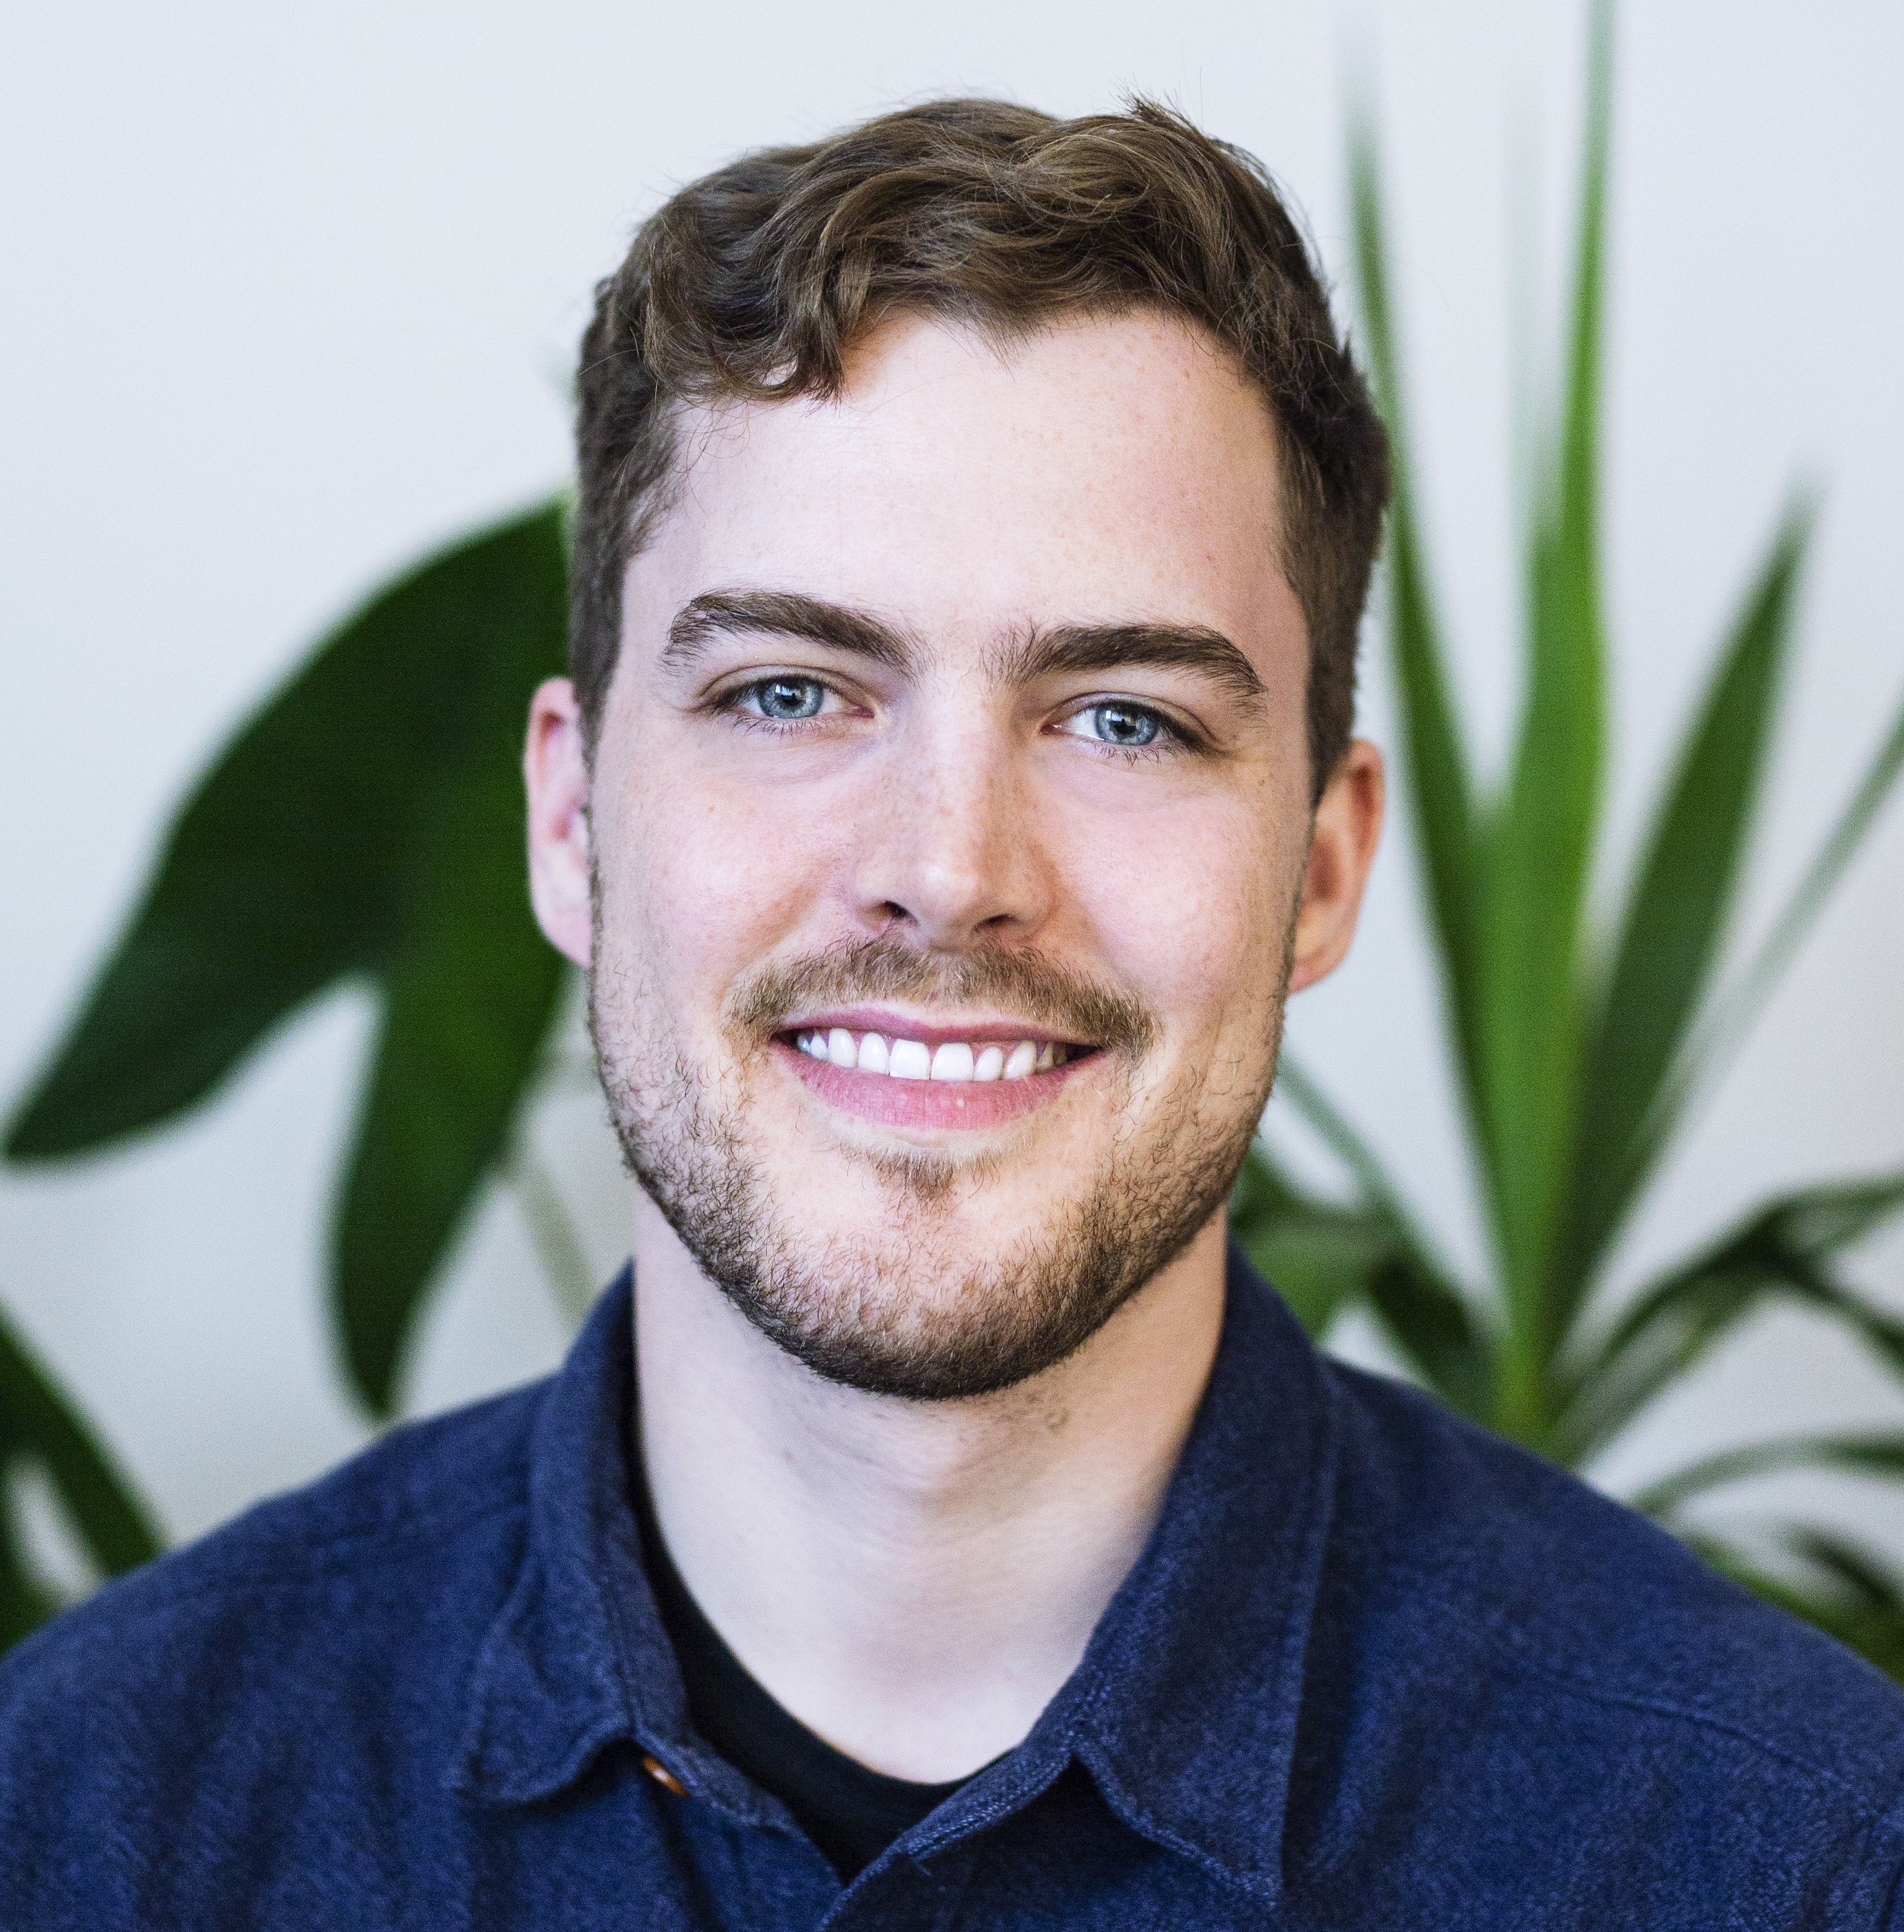
\includegraphics[width=\linewidth,height=2.5cm, keepaspectratio]{figures/bren096.jpg}
    \caption{Brendan Keith\\ Brown University}
  \end{subfigure}
  \hfill
  \begin{subfigure}[b]{2.75cm}
    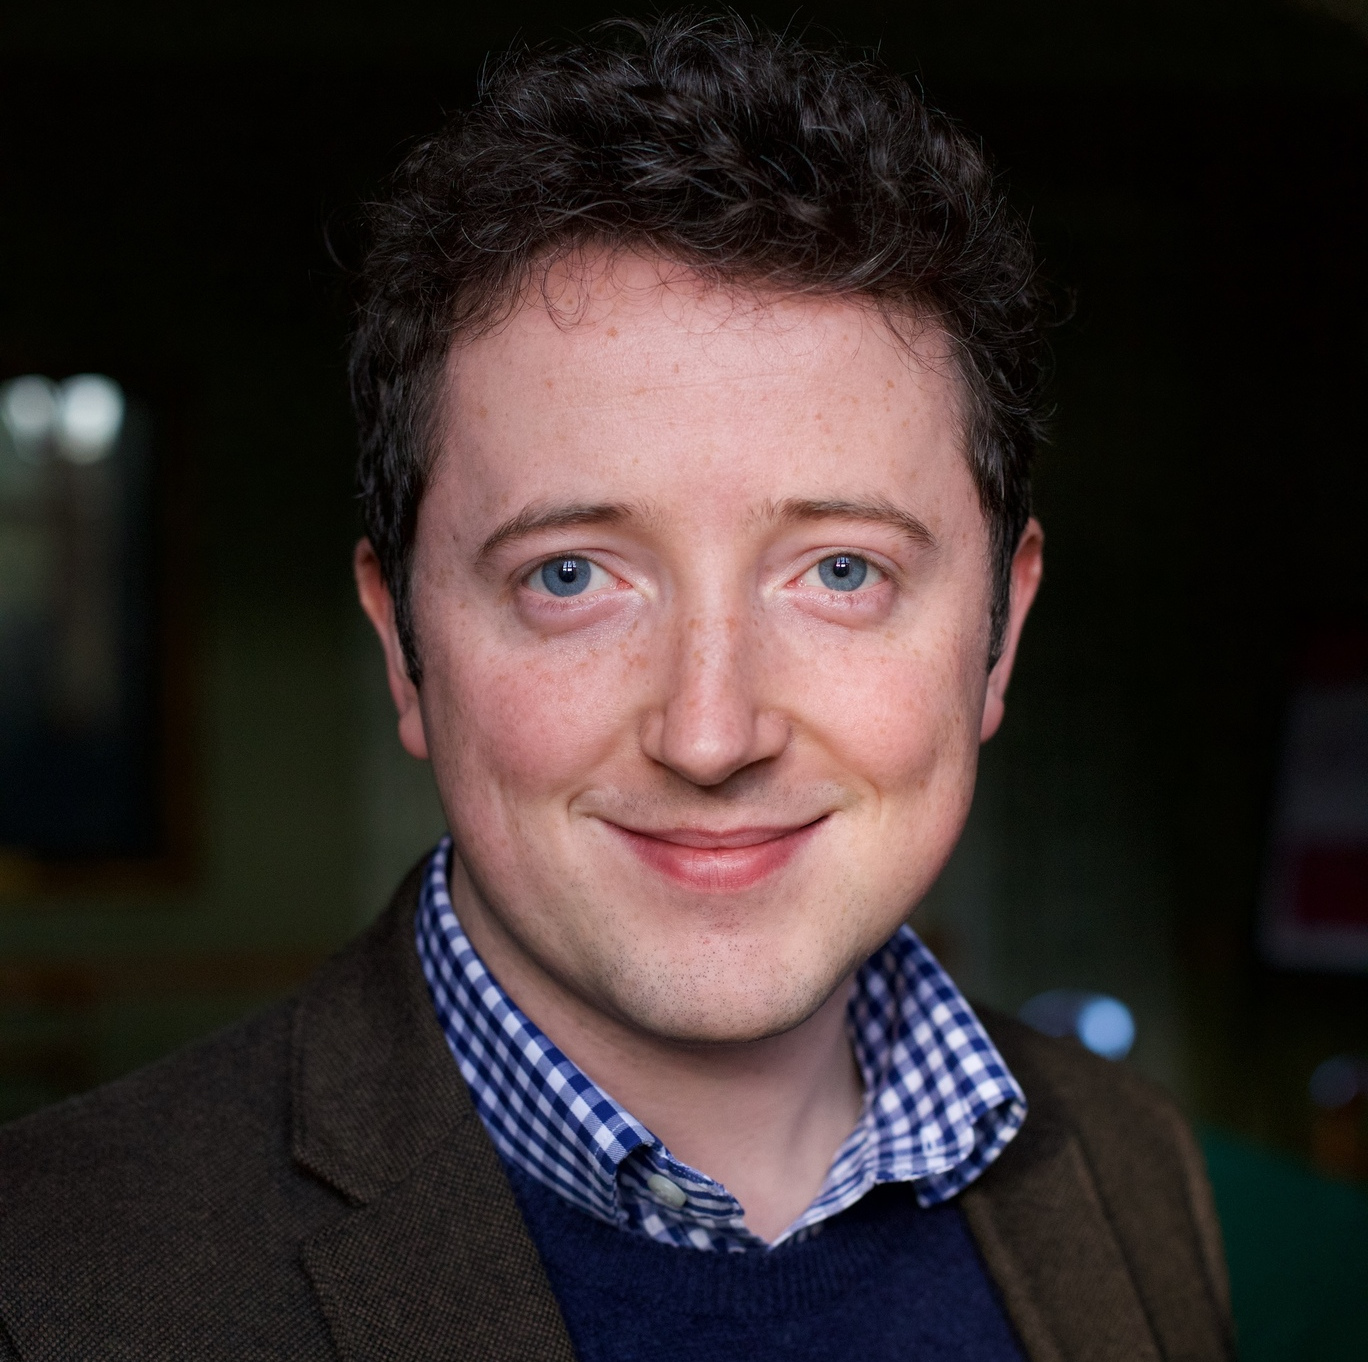
\includegraphics[width=\linewidth,height=2.5cm, keepaspectratio]{figures/patrick.jpg}
    \caption{Patrick E. Farrell\\ Oxford University}
  \end{subfigure}
  \hfill
  \begin{subfigure}[b]{2.75cm}
    
\includegraphics[width=\linewidth,height=2.5cm, keepaspectratio]{figures/joergen.png}
    \caption{Jorgen S. Dokken\\ Simula Research Lab}
  \end{subfigure}
   \hfill
  \begin{subfigure}[b]{3.2cm}
    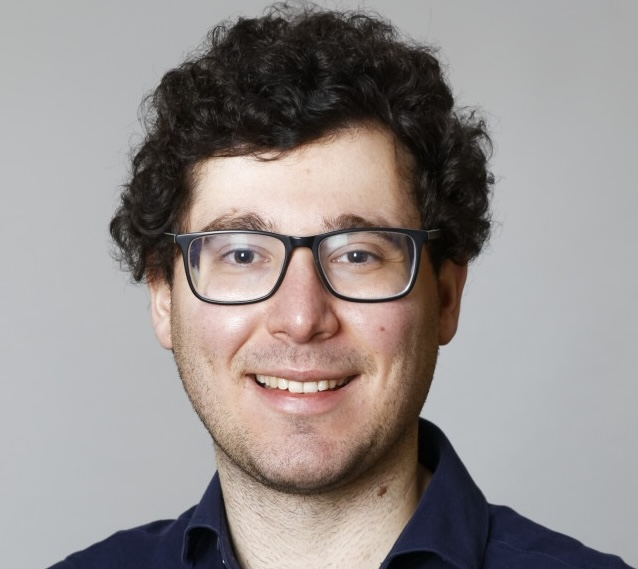
\includegraphics[width=\linewidth,height=2.5cm, keepaspectratio]{figures/papadopoulos.jpg}
    \caption{Ioannis Papadopoulos\\ Weierstra\ss-Institut}
  \end{subfigure}
\hspace{7em}	
%  \hfill
%  \begin{subfigure}[b]{0.19\textwidth}
%    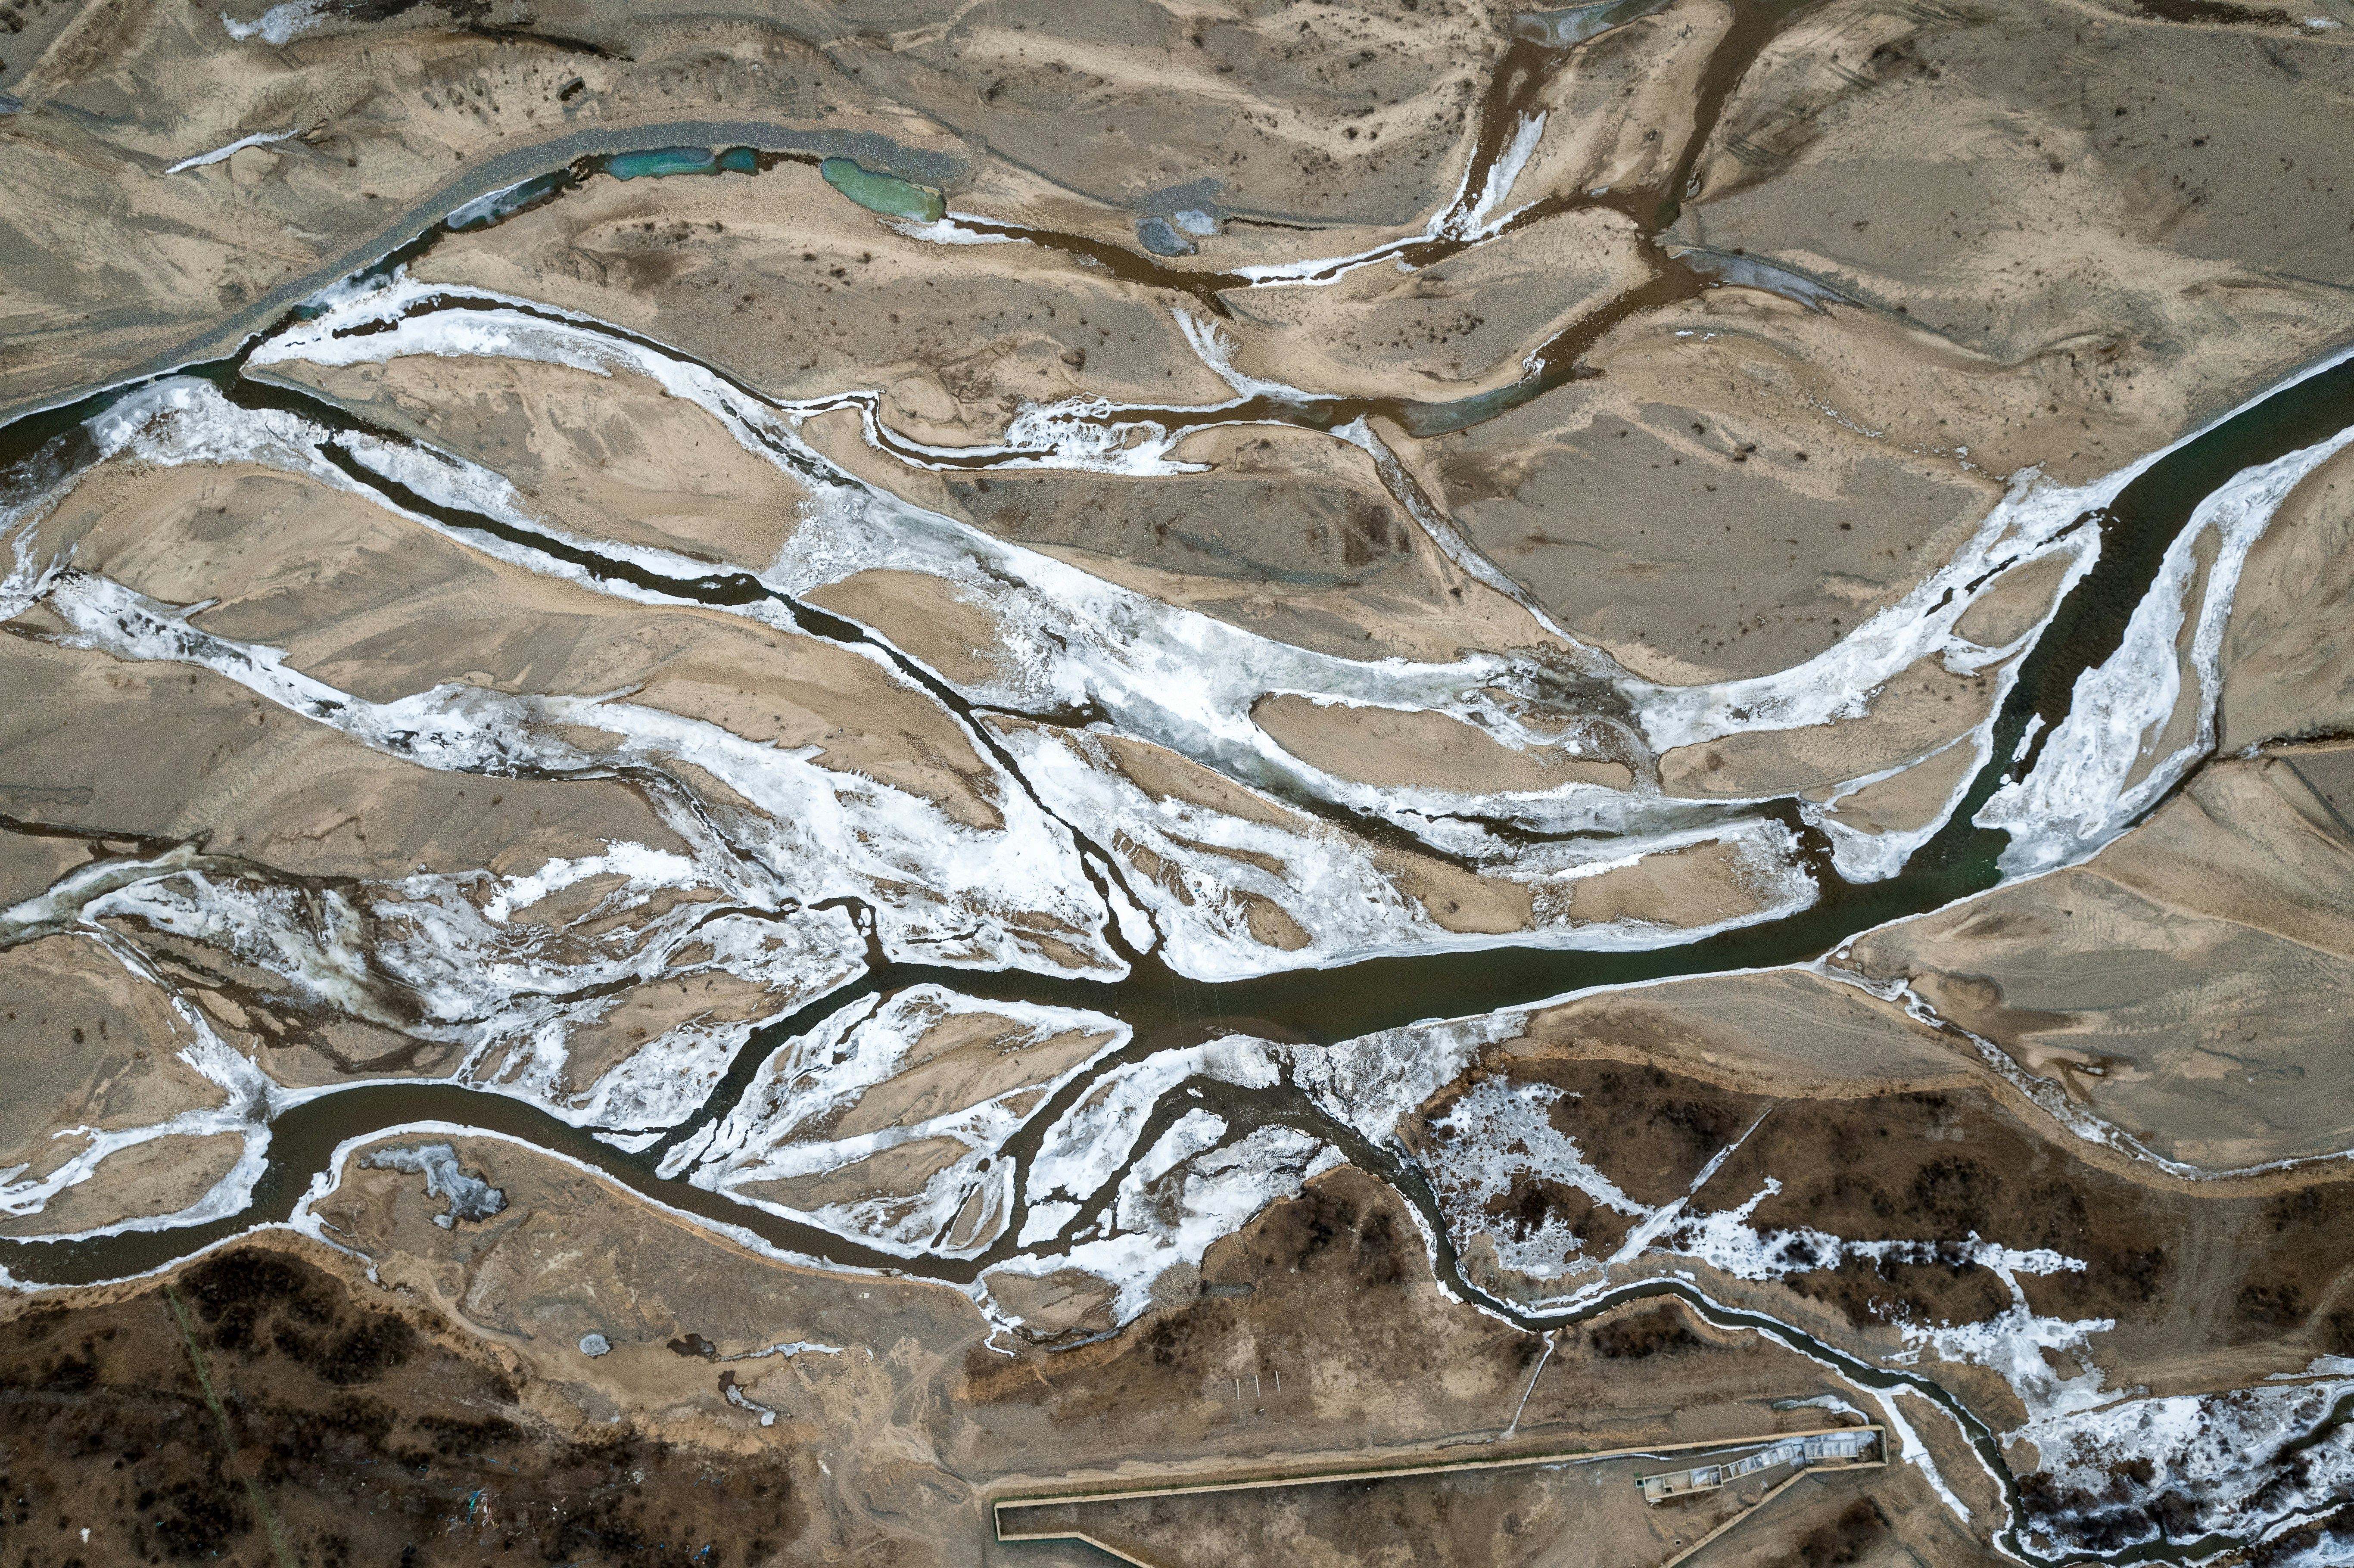
\includegraphics[width=\linewidth]{figures/rivers.jpg}
%    \caption{Diffusive Waves}
%  \end{subfigure}
\end{figure}\vspace{-4ex}
{\tiny
\begin{thebibliography}{1}

\bibitem{BKeith_TMSurowiec_2024}
{\sc B.~Keith and T.M.~Surowiec.}
\newblock Proximal Galerkin: A structure‐preserving finite element method for pointwise bound constraints
\newblock Found. Comut. Math. (2024), \url{https://doi.org/10.1007/s10208-024-09681-8}

\bibitem{JSDokken_etal_2025}
{\sc J.S.~ Dokken, P.E.~Farrell, B.~Keith, I.P.A.~Papadopolous and T.M.~Surowiec.}
\newblock The latent variable proximal point algorithm for variational problems with inequality constraints
\newblock Computer Methods in Applied Mechanics and Engineering,
Volume 445, 2025, 118181, \url{https://www.sciencedirect.com/science/article/abs/pii/S0045782525004530}
\end{thebibliography}
}
\end{frame}

\begin{frame}{Overview}
\tableofcontents
\end{frame}

\section{Introduction to Variational Inequalities}
\subsection{Motivation and context}\label{sec:motivation}
%\begin{frame}{Dirichlet's Principle}
%    \begin{enumerate}
%        \item History
%            \begin{enumerate}
%                \item Who invented it, when did it get its name, etc.
%            \end{enumerate}
%        \item Modern interpretation and a first variational inequality
%            \begin{enumerate}
%                \item Derivation of a variational inequality
%                    \begin{enumerate}
%                        \item The feasible set is nonempty, closed, and convex
%                        \item Existence via direct method
%                        \item The objective function is G\^{a}teaux differentiable
%                        \item Derivation of the VI
%                    \end{enumerate}
%            \end{enumerate}
%        \item Reformulation as a variational equation
%            \begin{enumerate}
%                \item Using a clever test function
%                \item Use lifting discussion see Chouly 2023, Poisson.
%            \end{enumerate}
%    \end{enumerate}
%\end{frame}


\begin{frame}{Dirichlet's Principle}

  \begin{minipage}{0.48\textwidth}
  \begin{beamercolorbox}[rounded=true, shadow=true, wd=\textwidth]{block body}
 \textit{The solution to Poisson's equation is the minimizer of a certain energy functional.}\\
  
  \visible<2->{Early observations due to Thomson and Gau\ss.}\\
  
  \visible<3->{Riemann named it after his teacher Dirichlet.}\\
  
  \visible<4->{Hilbert justified Riemann's use of Dirichlet's principle,\\ invents the Direct Method (1900-1905).}
     \end{beamercolorbox}
    \end{minipage}\hspace*{1.75cm}
    \begin{minipage}{0.3\textwidth}
  \centering
 \begin{figure}
  \centering\vspace{1ex}
  \only<1-3>{\begin{minipage}[b]{0.45\textwidth}
    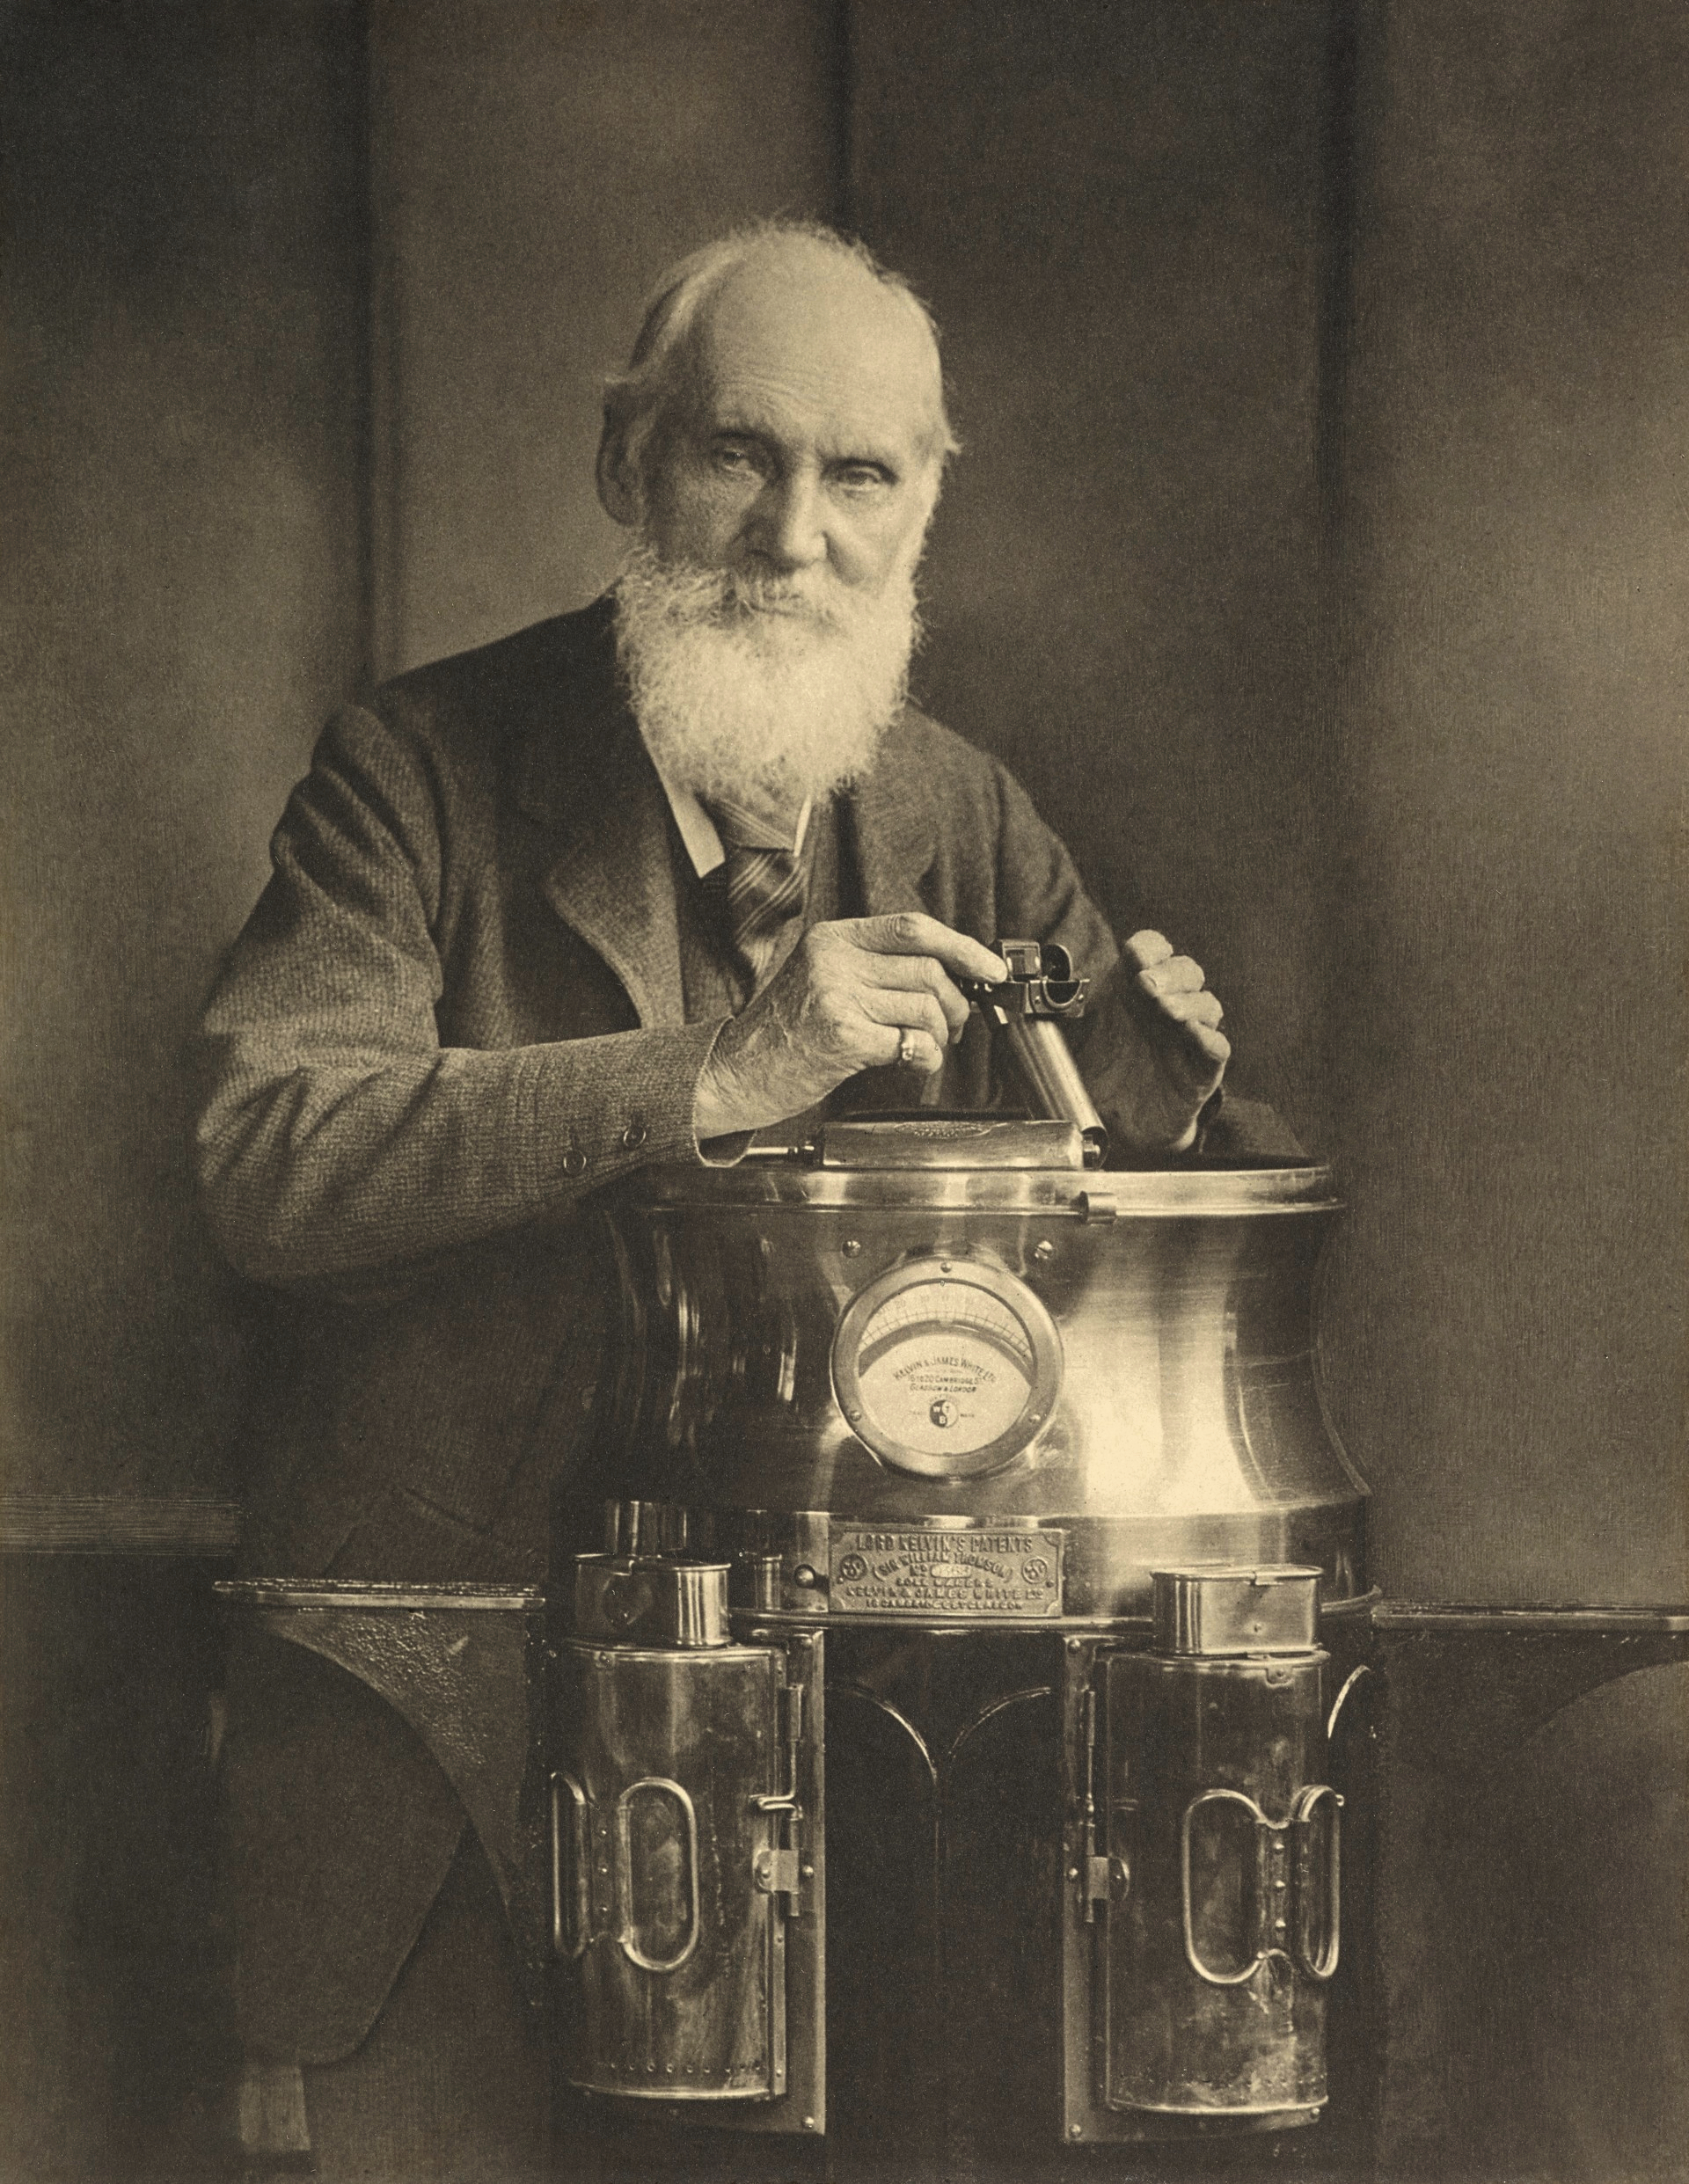
\includegraphics[width=\linewidth]{figures/kelvin.jpg}
    \captionof*{figure}{\tiny W. Thomson}
  \end{minipage}}%
   \only<4->{\begin{minipage}[b]{0.43\textwidth}
    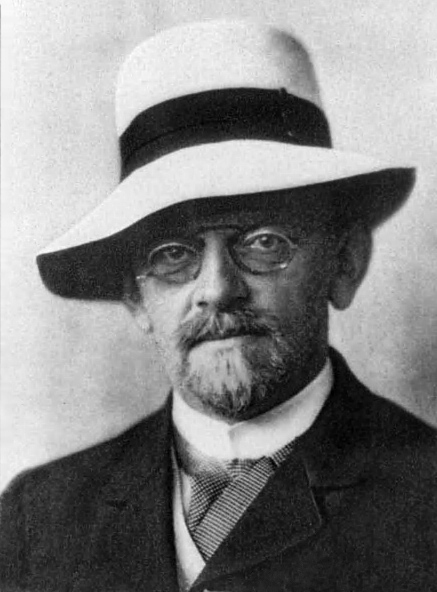
\includegraphics[width=\linewidth]{figures/Hilbert.jpg}
    \captionof*{figure}{\tiny \alert{D. Hilbert}}
  \end{minipage}}
  \hfill
  \begin{minipage}[b]{0.455\textwidth}
    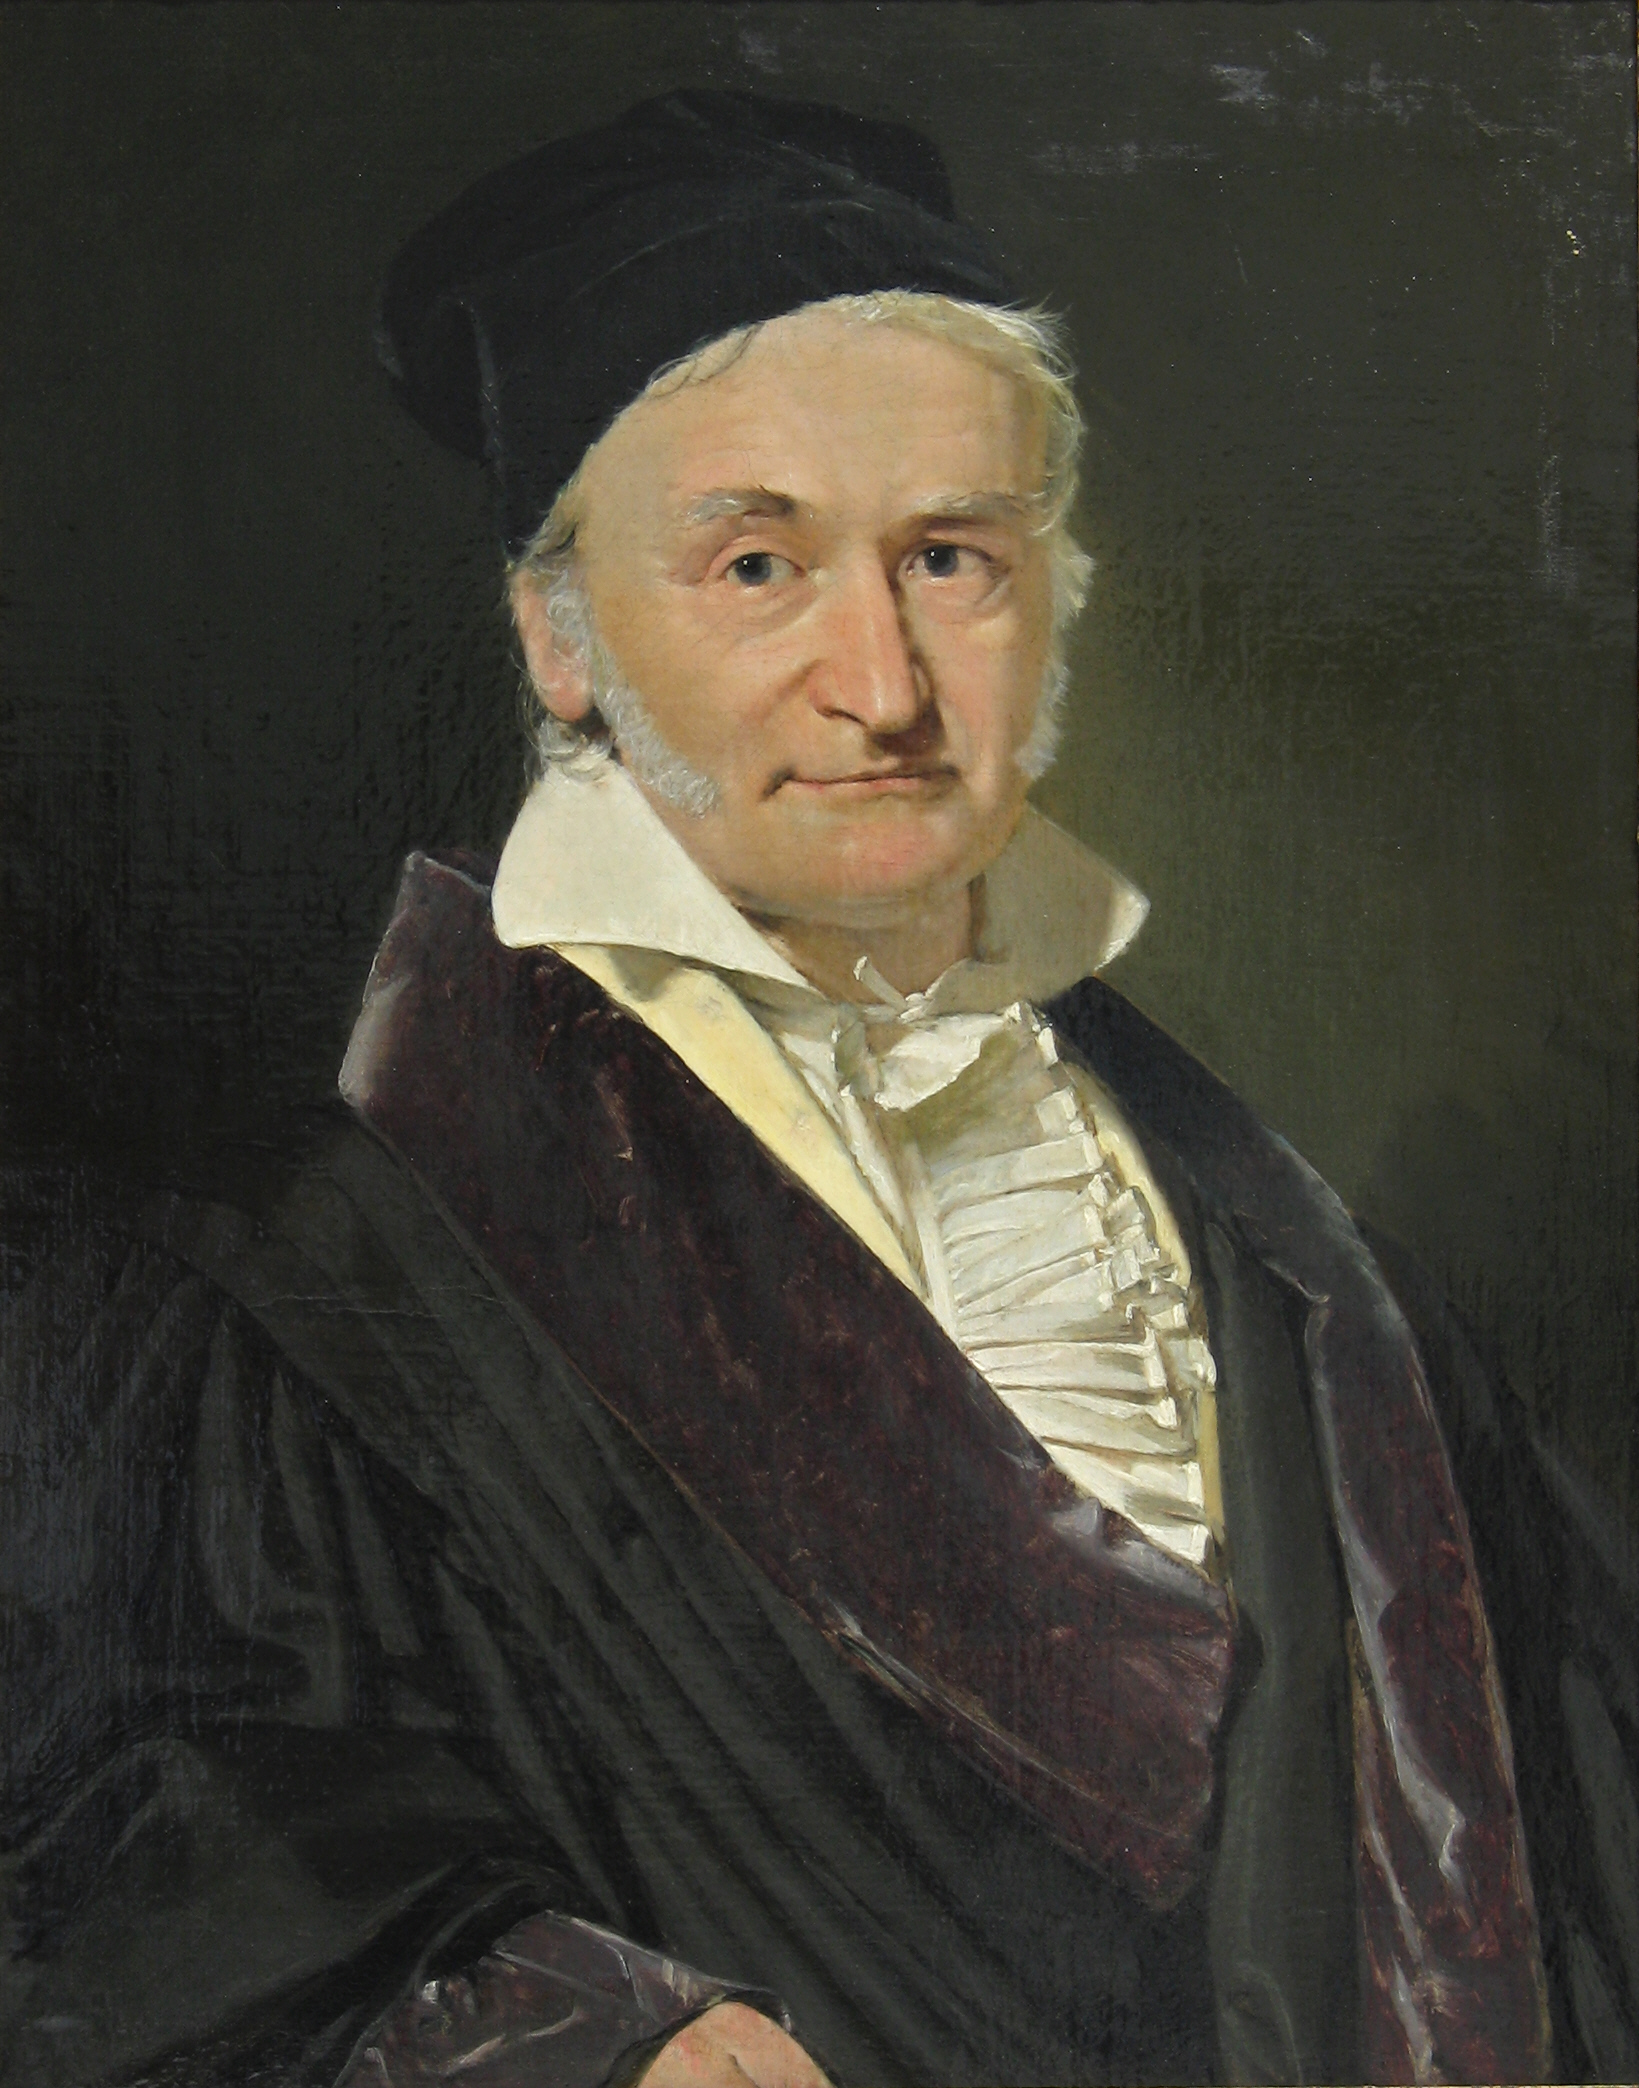
\includegraphics[width=\linewidth]{figures/gauss.jpg}
    \captionof*{figure}{\tiny C.F. Gau\ss }
  \end{minipage}
  \vspace{1em}
  \begin{minipage}[b]{0.45\textwidth}
    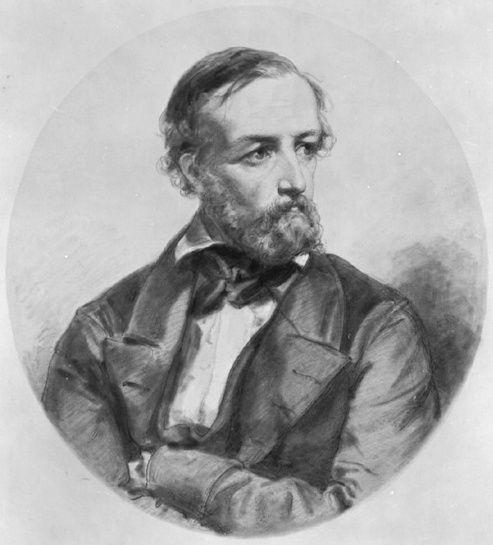
\includegraphics[width=\linewidth]{figures/dirichlet.jpg}
    \captionof*{figure}{\tiny P.G.L. Dirichlet}
  \end{minipage}
  \hfill
  \begin{minipage}[b]{0.45\textwidth}
    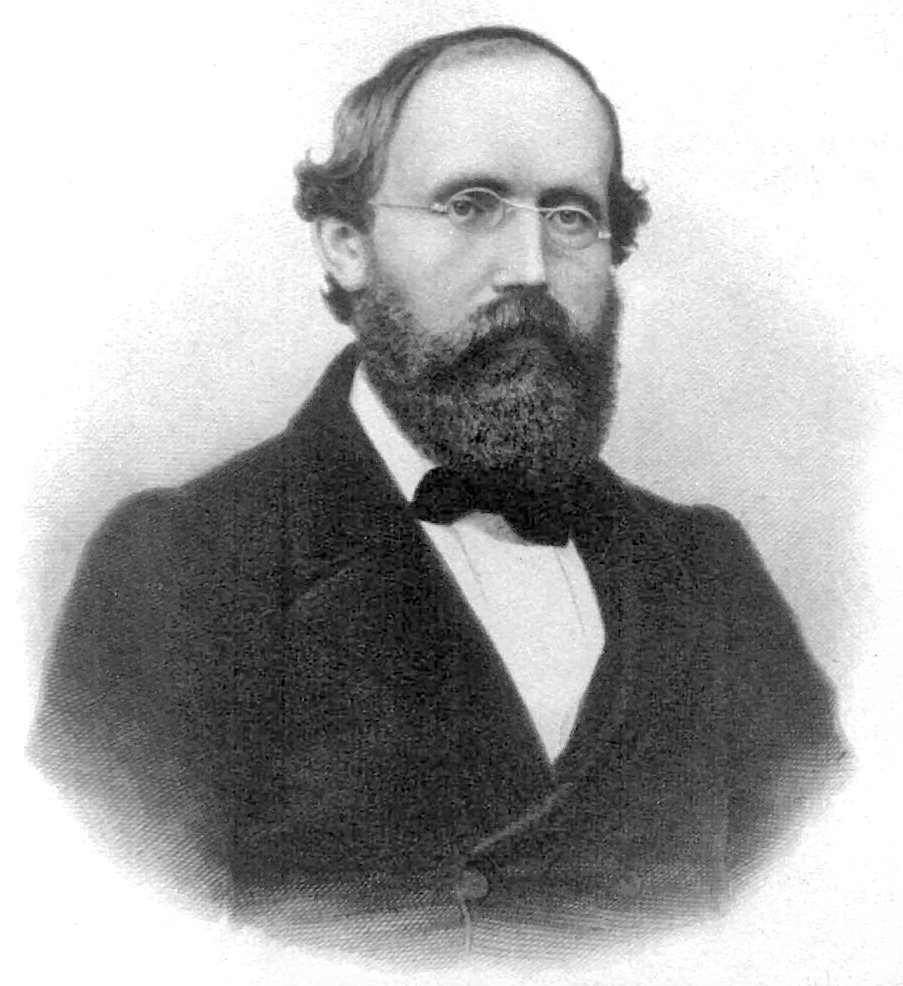
\includegraphics[width=\linewidth]{figures/riemann.jpg}
    \captionof*{figure}{\tiny B. Riemann}
  \end{minipage}
\end{figure}
    \end{minipage}
\end{frame}

\begin{frame}\frametitle{Dirichlet's Principle: Modern Form}
% We seek a minimizer $u$ of the energy functional:
% \begin{equation*}
% 	E(v)
% 	=
% 	\frac{1}{2}
% 	\int_\Omega |\nabla v|^2 \dd x
% 	-
% 	\int_\Omega v f \dd x
% 	\,,
% \end{equation*}
% over the \textbf{closed convex cone} defined by  
% \[
% K = \{ v \in H^1_0(\Omega) \mid v \geq 0 \text{~a.e.}\}.
% \] 
% (Displacements $v \ge 0$, the obstacle)

 \begin{beamercolorbox}[rounded=true, shadow=true, wd=\textwidth]{block body}
\visible<1->{For any $f\in L^2(\Omega)$ and $g\in H^{1/2}(\Gamma)$, the (weak) solution of Poisson's equation over an open bounded Lipschitz domain $\Omega \subset \mathbb{R}^n$ with boundary $\Gamma$
 \begin{equation}
 \label{eq:PoissonEquation}\tag{Poisson Problem}
 	-\Delta u = f
 	\quad \text{in~} \Omega,
 	\qquad
 	u = g \quad \text{on~} \Gamma,
 \end{equation}}\visible<2->{
 is the \textbf{$H^1(\Omega)$-minimizer} of the total energy functional,
 \begin{equation}
 \label{eq:DirichletEnergy}\tag{Dirichlet Energy}
 	E(v)
 	=
 	\frac{1}{2}
 	\int_\Omega |\nabla v|^2 \dd x
 	-
 	\int_\Omega f v \dd x
 	\,,
 \end{equation}}\visible<3->{
 when confined to the \textbf{constraint set} $H^1_g(\Omega) = g + H^1_0(\Omega) = \{ v \in H^1(\Omega) \mid v = g \text{~on~} \partial \Omega\}$.}
\end{beamercolorbox}

%\visible<4->{
% \begin{beamercolorbox}[rounded=true, shadow=true, wd=\textwidth]{block title}\centering
% We sketch the proof. The arguments extend to much more complicated examples!
% \end{beamercolorbox}
%}
\end{frame}

%\begin{frame}\frametitle{The Direct Method}
%
% \begin{beamercolorbox}[rounded=true, shadow=true, wd=\textwidth]{block body}
% There are a few basic steps
% \begin{enumerate}
% \item Start with a minimizing sequence $\left\{v_k\right\}$ meaning  \[\inf_{v \in H^1_g(\Omega)} E(v) = \liminf_{k \to +\infty} E(v_k).\] 
% \item For some topology $\tau$, show $\left\{v_k\right\}$ admits a $\tau$-convergent subsequence $\left\{v_{k_l}\right\}$ to some $\bar{v}$.
% \item Argue that $\bar{v}$ is a feasible point, i.e. $\bar{v} \in H^1_g(\Omega)$.
% \item Show that $E$ is $\tau$-lower semicontinuous. 
% \end{enumerate}
% \end{beamercolorbox}
%
%\visible<2->{
% \begin{beamercolorbox}[rounded=true, shadow=true, wd=\textwidth]{block title}
%% This works because
%  \[
% \inf_{v \in H^1_g(\Omega)} E(v) = \liminf_{k \to +\infty} E(v_k) =  \liminf_{l \to +\infty} E(v_{k_l}) \ge E(\bar{v}) \ge  \inf_{v \in H^1_g(\Omega)} E(v).
% \]
%  \end{beamercolorbox}}
% 
%\end{frame}

%\begin{frame}\frametitle{The Direct Method}
% \begin{beamercolorbox}[rounded=true, shadow=true, wd=\textwidth]{block body}
% \visible<1->{We would like to \alert{prove} the existence of a solution to the optimization problem:
% \[
% \inf_{u \in H^1_g(\Omega)} E(u).
% \]
%We use the \alert{Direct Method of the Calculus of Variations}. For simplicity $g \equiv 0$, $f \ne 0$.}
% \end{beamercolorbox}
% 
% \visible<2->{
%  \begin{beamercolorbox}[rounded=true, shadow=true, wd=\textwidth]{block body}
%% \begin{enumerate}
%% \item 
%\visible<2->{$E$ may not be bounded from below here. However,}
%\visible<3->{for any $v \in H^1_0(\Omega)$, $E(v)$ is finite and 
% \[
% E(v) \ge \frac{1}{2} \| \nabla v \|^2_{L^2} - \| v \|_{L^2} \|f\|_{L^2} \ge \frac{1}{2} \| \nabla v \|^2_{L^2} - C \|\nabla v \|_{L^2} \| f \|_{L^2}
% \]}\vspace*{-1ex}
%% \item 
%
% \visible<4->{This means, if $\|v\|_{H^1_0} \to +\infty$, then $E(v) \to +\infty$, i.e., $E$ is \alert{$H^1_0(\Omega)$-coercive}.\medskip
%% \item 
% }
% 
% \visible<5->{
% Thus, $N_0 := \left\{ v \in H^1_0(\Omega) \left| E(v) \le E(v_0) \right.\right\}$ for any $v_0 \in H^1_0(\Omega)$ is \alert{bounded in $H^1_0(\Omega)$}.}
%% \end{enumerate}
% \end{beamercolorbox}
% }
%\end{frame}

%\begin{frame}\frametitle{The Direct Method}
% \visible<1->{\begin{beamercolorbox}[rounded=true, shadow=true, wd=\textwidth]{block body}
%\visible<1->{If  $\{v_k\} \subset H^1_0(\Omega)$ is a minimizing sequence, then $v_k \in N_0$ for large $k$.\medskip
%
%Thus, $\{v_k\}$ is a \alert{bounded sequence}.\medskip
%}
%
%\visible<2->{$H^1_0(\Omega)$ is Hilbert $\Rightarrow$ bounded sequences admit \alert{weakly convergent subsequences}.\medskip
%
%\visible<3->{Hence, there exists $\{v_{k_l}\} \subset \{v_k\}$ and $\bar{v} \in H^1_0(\Omega)$ such that $v_{k_l} \rightharpoonup \bar{v}$ (weakly in $H^1_0(\Omega))$.
%
%\rule{\linewidth}{0.4pt}\medskip
%
%}
%
%
%\visible<4->{
%$E$ is the sum of a convex continuous function and a continuous linear functional.\medskip
%}
%
%\visible<5->{
% We can thus easily show that $E$ is \alert{weakly lower-semicontinuous}, meaning
% \[
% \forall v \in H^1_0(\Omega), \forall \{v_k\} \subset H^1_0(\Omega) : v_k \rightharpoonup v \quad\text{ we have }\quad \liminf_{k \to +\infty} E(v_k) \ge E(v).
% \]
%}\vspace{-2ex}
%
%\visible<6->{
%This completes the proof, i.e., $u = \bar{v}$ is a minimizer of $E$ over $H^1_0(\Omega)$.
%}
%}
% \end{beamercolorbox}
% }
%\end{frame}

%\begin{frame}\frametitle{Optimality Conditions}
% \visible<1->{\begin{beamercolorbox}[rounded=true, shadow=true, wd=\textwidth]{block body}
%  \visible<1->{The objective $E$ is \alert{strongly convex}: There is a $c > 0$ for all $u,v \in H^1_0(\Omega)$ and $\lambda \in [0,1]$
%  \[
%  E(\lambda u + (1-\lambda) v) \le \lambda E(u) + (1-\lambda) E(v) - c \lambda (1 - \lambda) \| u - v \|^2_{H^1_0}.
%  \]
%  }\vspace{-2ex}
%  
%  \visible<2->{
%  This makes it easy to show that the minimzer of $E$ is unique. But where's the PDE?
%  }\medskip
%  
% \visible<3->{
% Observe: 
% \begin{enumerate}
% \item \visible<3->{
%  For $v, w \in H^1_g(\Omega)$, $\lambda \in (0,1)$, we have $( \lambda v + (1-\lambda) w)|_{\Gamma} = \lambda g + (1-\lambda) g = g$.
%  \item This means the feasible set $H^1_g(\Omega)$ is convex. (Easy to show $\ne\emptyset$ and closed).
% }
%\item \visible<4->{
% For any $v \in H^1_g(\Omega)$ and $\tau > 0$ we have 
% \[
% E( u + \tau v) = E(u) + \tau [(\nabla u, \nabla v)_{L^2} - (f,v)_{L^2}] + \frac{\tau^2}{2} \| \nabla v \|^2_{L^2}
% \]
% }\vspace{-3ex}
% \end{enumerate}
% }
% \end{beamercolorbox}}
%\end{frame}

%\begin{frame}\frametitle{Optimality Conditions}
% \visible<1->{\begin{beamercolorbox}[rounded=true, shadow=true, wd=\textwidth]{block body}
% Consider the definition of our unique minimizer $u$: 
% \[
% E(u) \le E(v) \quad \forall v \in H^1_g(\Omega).
% \]
% 
% \visible<2->{
% Since $H^1_g(\Omega)$ is a convex set, $\lambda v + (1-\lambda) u = u + \lambda (v - u) \in H^1_g(\Omega)$ for all $v \in H^1_g(\Omega)$.
% }\medskip
% 
%  \visible<3->{
%  Then for fixed arbitrary $v \in H^1_g(\Omega)$, we have:
%  \[
%  E(u) \le E(u + \lambda (v - u) ) = E(u) + \lambda [(\nabla u, \nabla [v-u])_{L^2} - (f,v-u)_{L^2}] + \frac{\lambda^2}{2} \| \nabla [v-u] \|^2_{L^2}
%  \] }\visible<4->{and hence,
%  \[
% \lambda [(\nabla u, \nabla [v-u])_{L^2} - (f,v-u)_{L^2}] \ge o(\lambda) 
%  \]}\visible<5->{Divide by $\lambda > 0$ and let $\lambda \to 0$.
%  }
% 
% \end{beamercolorbox}}
%\end{frame}

\begin{frame}\frametitle{A First Variational Inequality}
 \visible<1->{\begin{beamercolorbox}[rounded=true, shadow=true, wd=\textwidth]{block body}
 \visible<1->{The following \alert{variational inequality} characterizes our solution $u$:
 \[
 (\nabla u, \nabla [v-u])_{L^2} \ge  (f,v-u)_{L^2} \quad \forall v \in H^1_g(\Omega)
 \]
 It states: \textit{The directional derivative of $E$ at $u$ in any feasible direction $v - u$ is non-negative.}
 }\medskip
 
\visible<2->{
In this simple example, we have, for any $v \in H^1_g(\Omega)$ and $w \in H^1_0(\Omega)$, $v + w \in H^1_g(\Omega)$.
}\medskip
 
\visible<3->{
This means $u \in H^1_g(\Omega)$ solves
 \[
 (\nabla u, \nabla w)_{L^2} =  (f,w)_{L^2} \quad \forall v \in H^1_0(\Omega),
 \]
 which brings us back to Poisson. (use $u + w$ and $u-w$ in the VI)
 }
  \end{beamercolorbox}}
  
\visible<4->{\begin{beamercolorbox}[rounded=true, shadow=true, wd=\textwidth]{block title}
\centering  But what about more complicated feasible sets?
\end{beamercolorbox}}
\end{frame}

\subsection{Variational Inequalities}



%\begin{frame}{Pointwise Inequality Constraints}
% \visible<1->{\begin{beamercolorbox}[rounded=true, shadow=true, wd=\textwidth]{block body}
%Given $u \in H^1(\Omega)$ with $u|_{\Gamma} = g$ we look for solutions satisfying a \alert{pointwise inequality}:
% \[
%  u \ge \varphi \quad \text{almost everywhere (a.e.) on } \Omega.
% \]
% Denote this \alert{feasible set} by $K$.
% \end{beamercolorbox}}
% 
% \visible<2->{\begin{beamercolorbox}[rounded=true, shadow=true, wd=\textwidth]{block title}
% \centering Are constraints like this even relevant?
% \end{beamercolorbox}
% }
%\end{frame}

\begin{frame}\frametitle{The Signorini Problem}
\begin{minipage}{0.55\linewidth}
\visible<1->{
\begin{beamercolorbox}[rounded=true, shadow=true, wd=\textwidth]{block body}
Signorini (1959), analyzed by Fichera (1963).\\
 
The essential first problem in contact mechanics.\\
 
Models the deformation of a linear elastic body in the presence of a contact boundary constraint.
\end{beamercolorbox}
}\visible<2->{
\begin{beamercolorbox}[rounded=true, shadow=true, wd=\textwidth]{block body}
\visible<2->{$\Omega \subset \mathbb{R}^3$, $\Gamma$ split into two disjoint subsets.}
\visible<2->{$\Gamma = \overline{ \Gamma_\mathrm{D} \cup \Gamma_\mathrm{T} }$ with\\
$\Gamma_D$ for \textbf{d}isplacement\\
$\Gamma_{T}$ for \textbf{t}raction boundary conditions.}
\end{beamercolorbox}}
\end{minipage}\hspace{4ex}
\begin{minipage}{0.3\linewidth}
 \centering
 \begin{figure}
  \centering\vspace{1ex}
  \visible<1->{\begin{minipage}[b]{0.45\textwidth}
    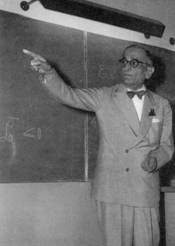
\includegraphics[width=\linewidth]{figures/Antonio_Signorini.jpg}
    \captionof*{figure}{\tiny A. Signorini}
  \end{minipage}}%
  \hfill
  \begin{minipage}[b]{0.46\textwidth}
    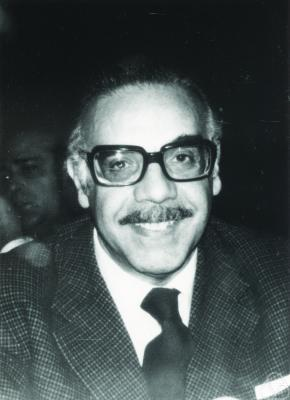
\includegraphics[width=\linewidth]{figures/Gaetano_Fichera.jpg}
    \captionof*{figure}{\tiny G. Fichera}
  \end{minipage}
\end{figure}\vspace{-8ex}
\begin{figure}
	\centering
	\begin{tikzpicture}
		\node at (-3.35,0) {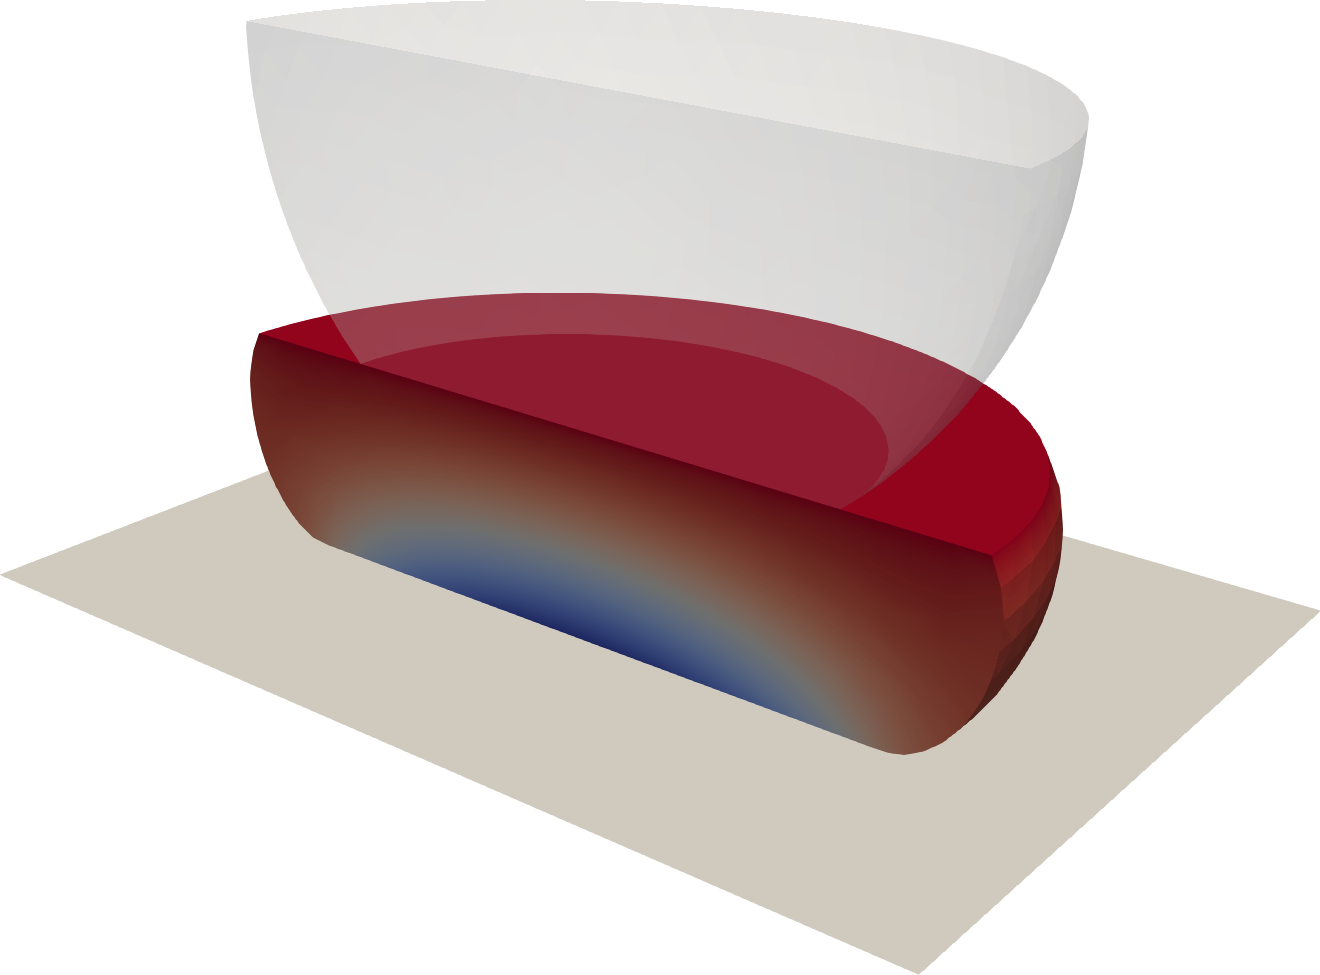
\includegraphics[height=1.25in]{figures/contact.png}};
    \end{tikzpicture}
\end{figure}
\end{minipage}
\end{frame}

\begin{frame}\frametitle{The Signorini Problem}
\begin{minipage}{0.55\linewidth}
\visible<1->{
\begin{beamercolorbox}[rounded=true, shadow=true, wd=\textwidth]{block body}
\visible<1->{State space:\vspace{-1.5ex}
\begin{equation*}
\label{eq:Signorini_V}
    V = \big\{ u \in H^1(\Omega,\mathbb{R}^3)
        \mid u = g \text{ on } \Gamma_\mathrm{D\textbf{}}
    \big\}
    \,,
\end{equation*}}\vspace{-4ex}

\visible<2->{Objective function:\vspace{-1.5ex}
\begin{equation*}
    J(u) =
    \frac{1}{2}\int_\Omega (\mathbb C \epsilon(u)) : \epsilon(u) \dd x
    -
    \int_\Omega f \cdot u \dd x
    \,,
\end{equation*}}\vspace{-2.5ex}

\visible<3->{Inequality constraints:\vspace{-1ex}
\begin{equation*}
 \alert{   K = \big\{ u \in V
        \mid u \cdot \tilde{n} \leq \phi_1 \text{ on } \Gamma_\mathrm{T}
    \big\} }
    \,.
\end{equation*}}\vspace{-4ex}
\end{beamercolorbox}
}\visible<4->{
\begin{beamercolorbox}[rounded=true, shadow=true, wd=\textwidth]{block body}\scriptsize
%Here, $\epsilon : H^1(\Omega,\mathbb{R}^3) \to L^2(\Omega,\mathbb{R}^{3\times 3}_{\mathrm{sym}})$, 
$\epsilon := (\nabla + \nabla^\top)/2$ symmetric gradient\smallskip
 
$\C \colon \mathbb{R}^{3\times 3}_{\mathrm{sym}} \to \mathbb{R}^{3\times3}_{\mathrm{sym}}$ sym.\ pos.-def.\ elasticity tensor\smallskip

$f \colon \Omega \to \mathbb{R}^3$ internal body force density\smallskip

$\phi_1 \colon \Gamma_\mathrm{T} \to \mathbb{R}_+$ gap function, $\tilde{n}$ normal to contact surface.
\end{beamercolorbox}}
\end{minipage}\hspace{4ex}
\begin{minipage}{0.3\linewidth}
 \centering
 \begin{figure}
  \centering\vspace{1ex}
  \visible<1->{\begin{minipage}[b]{0.45\textwidth}
    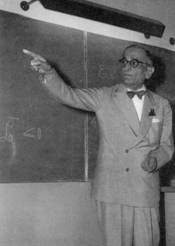
\includegraphics[width=\linewidth]{figures/Antonio_Signorini.jpg}
    \captionof*{figure}{\tiny A. Signorini}
  \end{minipage}}%
  \hfill
  \begin{minipage}[b]{0.46\textwidth}
    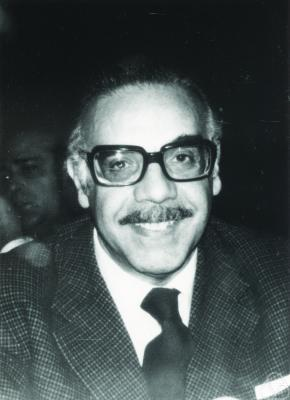
\includegraphics[width=\linewidth]{figures/Gaetano_Fichera.jpg}
    \captionof*{figure}{\tiny G. Fichera}
  \end{minipage}
\end{figure}\vspace{-8ex}
\begin{figure}
	\centering
	\begin{tikzpicture}
		\node at (-3.35,0) {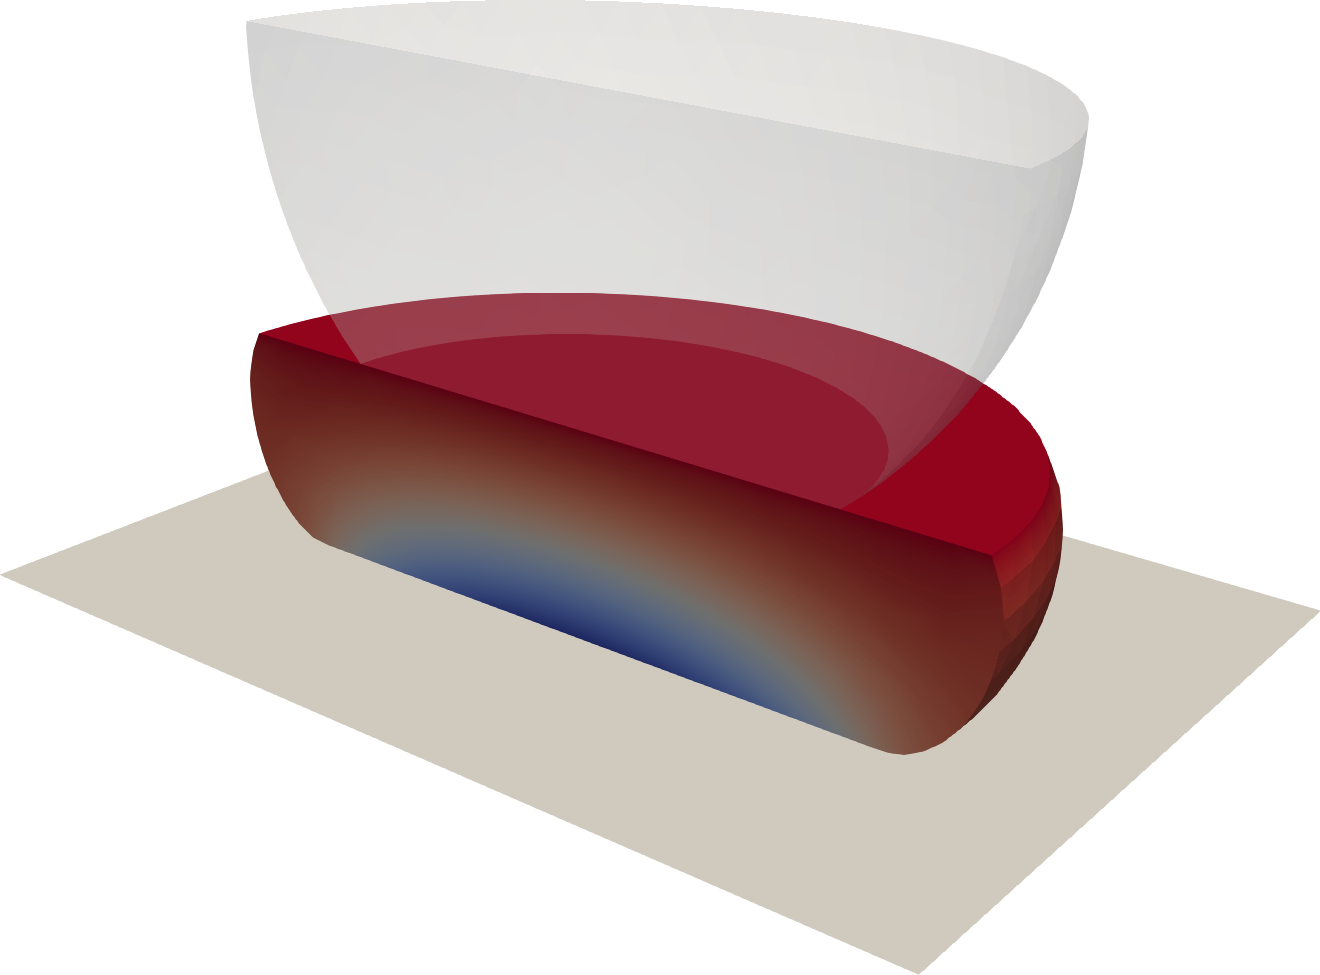
\includegraphics[height=1.25in]{figures/contact.png}};
    \end{tikzpicture}
\end{figure}
\end{minipage}
\end{frame}
%\hypertarget{example_1_alpha}{}
% \hyperlink{target_alpha}{\beamerbutton{Go to choice of $\alpha$}}
% \hyperlink{target}{\beamerbutton{Go to Finite Element Spaces}}
%  \hyperlink{target_alg}{\beamerbutton{Go to Algorithm and Convergence}}


\begin{frame}\frametitle{Gradient Constraints}
\begin{minipage}{0.55\linewidth}
\visible<1->{
\begin{beamercolorbox}[rounded=true, shadow=true, wd=\textwidth]{block body}
\footnotesize}\visible<1->{Often arise in \alert{Quasi-Variational Inequalities} (QVIs).\\
 
 }\visible<2->{
Major contributions by L. Prigozhin (modeling), J.F. Rodrigues (analysis), M. Hinterm\"uller \& C.N. Rautenberg (algorithms), and many others.\\
 
 }\visible<3->{
Diverse applications: 
\begin{itemize}
\item Elastic-plastic torsion problem
\item Sandpile growth
\item Magnetization in type-II superconductors
\item Hydrology 
\item Simplified stress constraints.
\end{itemize}}
\end{beamercolorbox}

%\visible<2->{
%\begin{beamercolorbox}[rounded=true, shadow=true, wd=\textwidth]{block body}
%\visible<2->{$\Omega \subset \mathbb{R}^3$, $\Gamma$ split into two disjoint subsets.}
%\visible<2->{$\Gamma = \overline{ \Gamma_\mathrm{D} \cup \Gamma_\mathrm{T} }$ with\\
%$\Gamma_D$ for \textbf{d}isplacement\\
%$\Gamma_{T}$ for \textbf{t}raction boundary conditions.}
%\end{beamercolorbox}}
\end{minipage}\hspace{4ex}
\begin{minipage}{0.3\linewidth}
 \centering
 \begin{figure}
  \centering\vspace{1ex}
  \visible<1->{\begin{minipage}[b]{0.38\textwidth}
    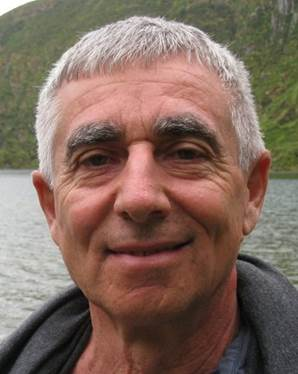
\includegraphics[width=\linewidth]{figures/Prigozhin.jpg}
    \captionof*{figure}{\tiny L. Prigozhin}
  \end{minipage}}%
  \hfill
  \begin{minipage}[b]{0.46\textwidth}
    \includegraphics[width=\linewidth]{figures/Rodrigues.jpg}
    \captionof*{figure}{\tiny J.F. Rodrigues}
  \end{minipage}
\end{figure}
 \begin{minipage}[b]{0.5\textwidth}
    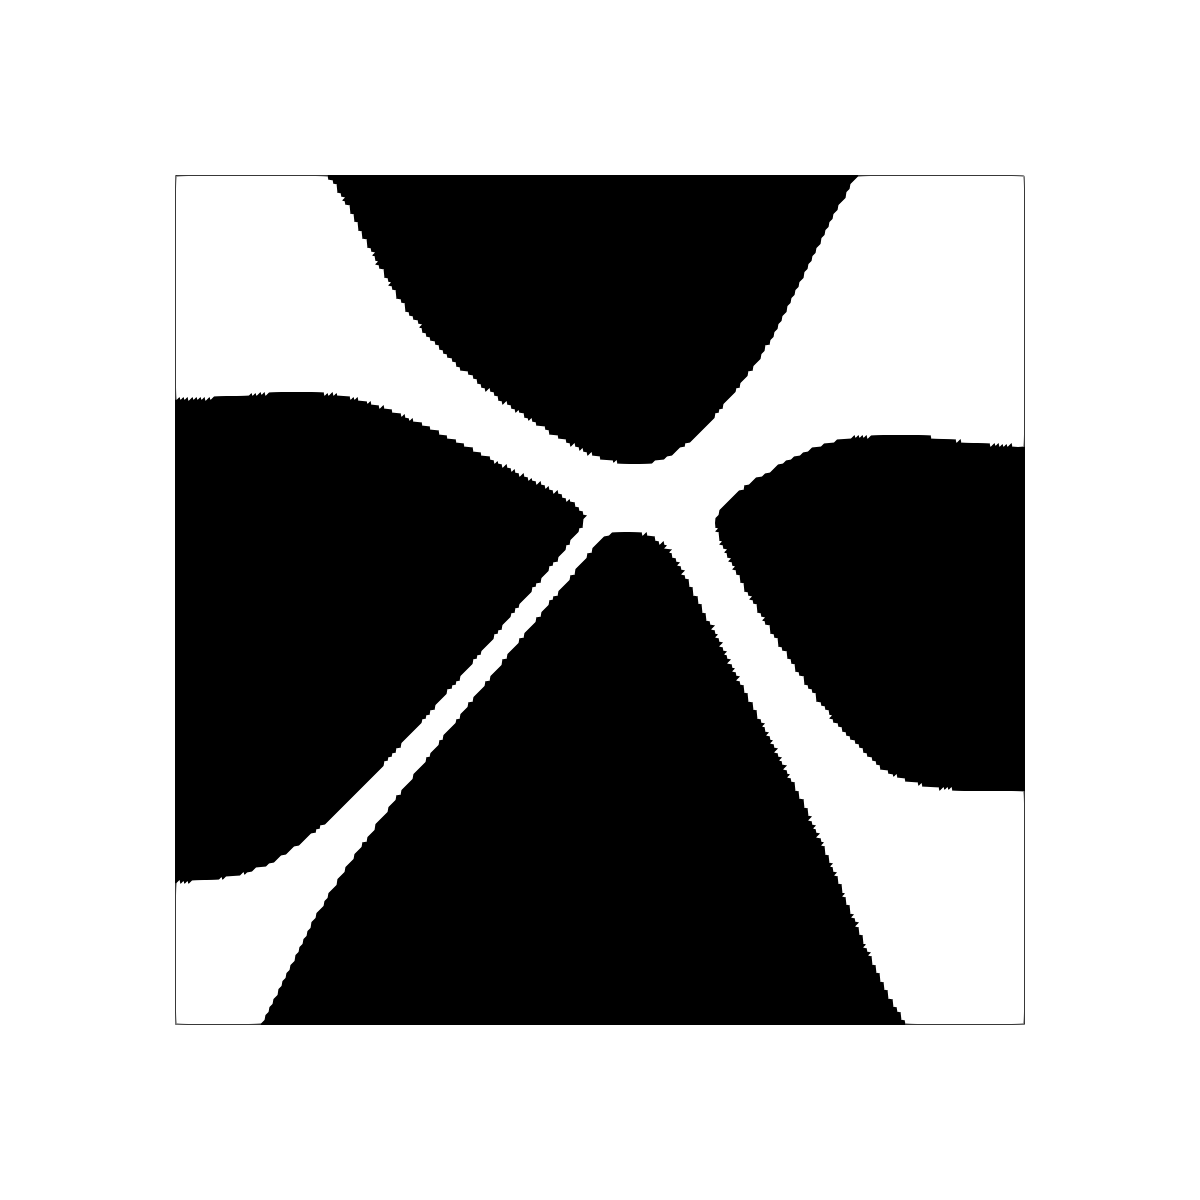
\includegraphics[width=\linewidth]{figures/global_feasible_active_set.png}
    \captionof*{figure}{\tiny Black: $|\nabla u| = \phi$.}
  \end{minipage}%
%  \hfill
%  \begin{minipage}[b]{0.6\textwidth}
    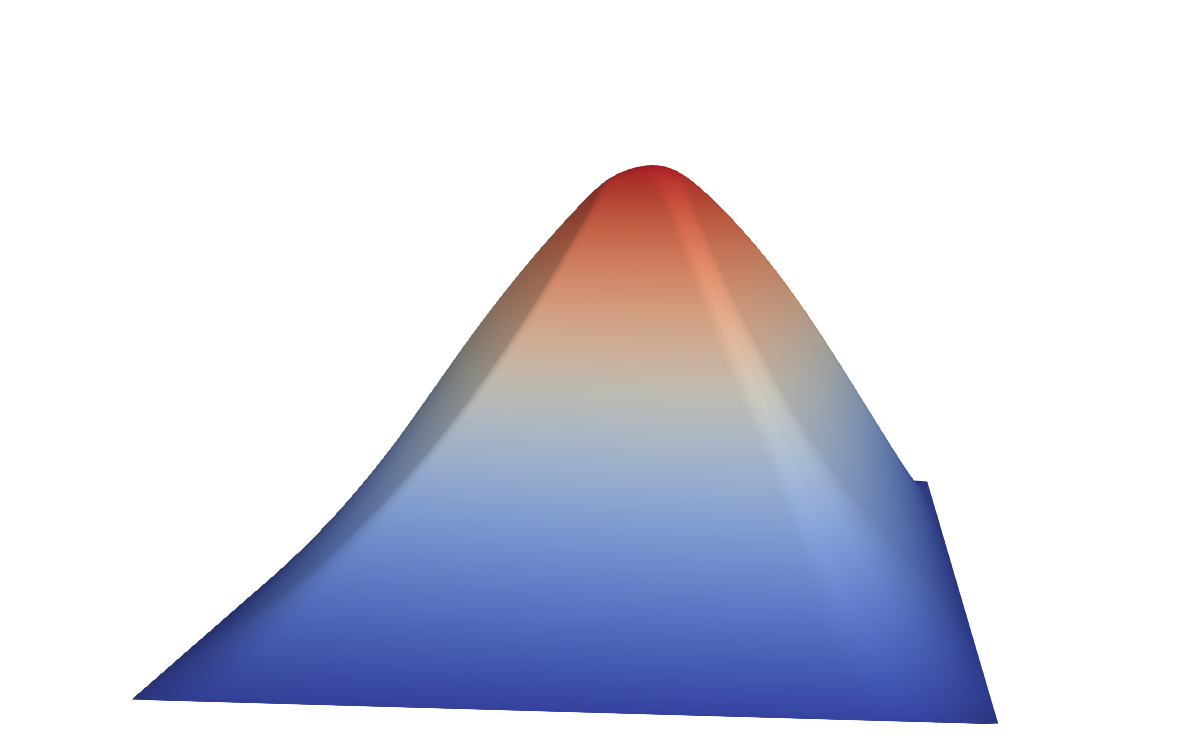
\includegraphics[width=0.8\linewidth]{figures/gradient_constraint_u.png}
%    \captionof*{figure}{\tiny State $u$}
%  \end{minipage}
%\begin{figure}
%	\centering
%	\begin{tikzpicture}
%		\node at (-5,0) {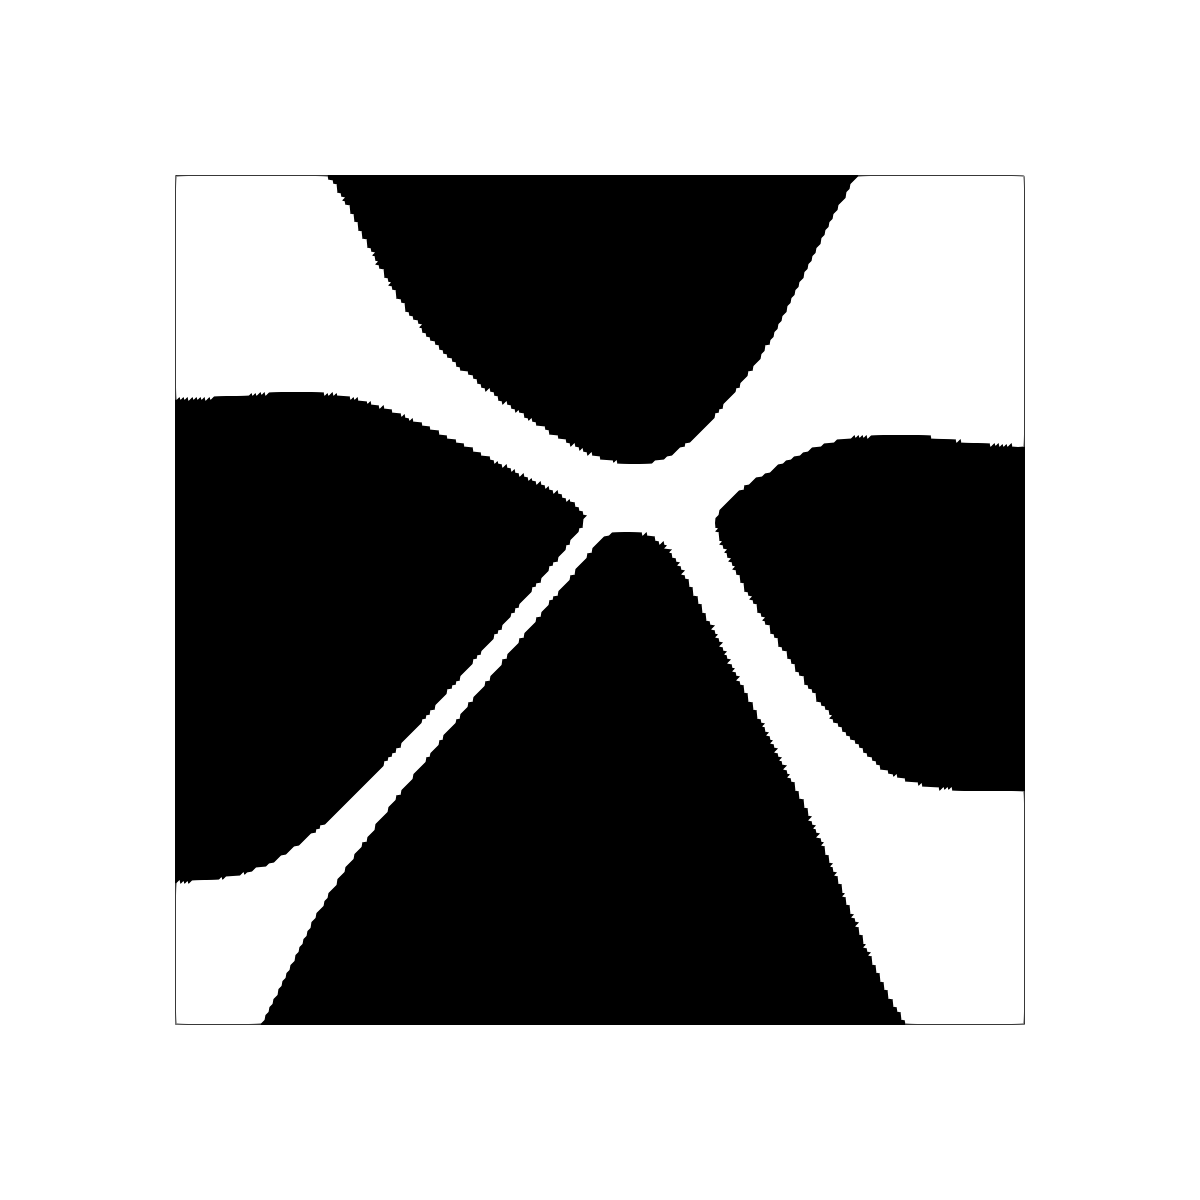
\includegraphics[height=1in]{figures/global_feasible_active_set.png}};\hspace{10ex}
%    \end{tikzpicture}\vspace{-8ex}
%	\begin{tikzpicture}
%		\node at (-2,-1) {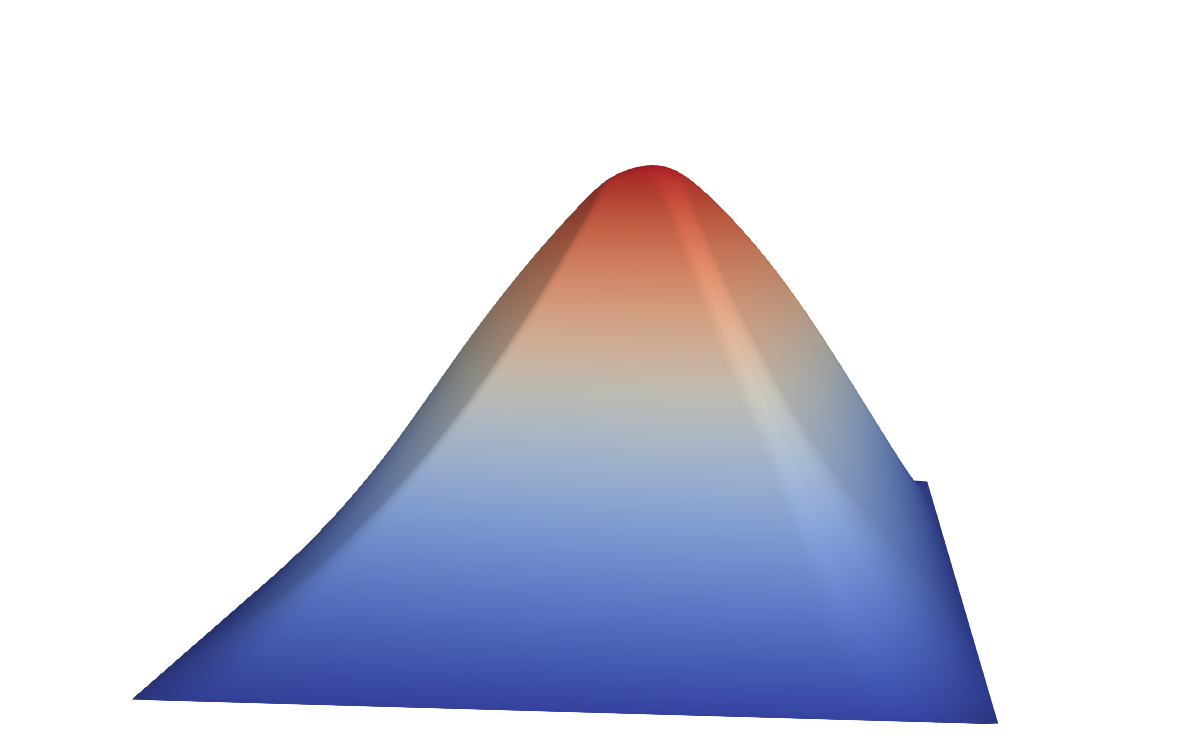
\includegraphics[height=1.25in]{figures/gradient_constraint_u.png}};
%    \end{tikzpicture}
%%\end{figure}
%  \end{minipage}
\end{minipage}
\end{frame}

\begin{frame}\frametitle{Gradient Constraints}
\begin{minipage}{0.55\linewidth}
\visible<1->{
\begin{beamercolorbox}[rounded=true, shadow=true, wd=\textwidth]{block body}
\footnotesize\visible<1->{Domain: $\Omega \subset \mathbb{R}^n$ open, bounded, Lipschitz\\

}\visible<2->{
State space: $V := W^{1,p}_0(\Omega)$ with $p \ge 2$\\

}\visible<3->{
Objective function:
 \begin{equation*}\label{eq:grad-ob}
     J(u) :=  \frac{1}{p} \int_{\Omega}|\nabla u|^p - f u \dd x
 \end{equation*}
Forcing term $f \in L^2(\Omega)$\medskip

}\visible<4->{
\alert{Inequality constraints:
\begin{equation}\label{eq:grad-constr}
K = \{ u \in H^1_0(\Omega) \mid |\nabla u| \le \phi \text{ a.e.\ in } \Omega \}\,.
\end{equation}
}
$\phi \in L^{\infty}(\Omega)$ : $\phi \ge \epsilon$ a.e.\ for constant $\epsilon > 0$.
}


\end{beamercolorbox}
}
%\visible<2->{
%\begin{beamercolorbox}[rounded=true, shadow=true, wd=\textwidth]{block body}
%\visible<2->{$\Omega \subset \mathbb{R}^3$, $\Gamma$ split into two disjoint subsets.}
%\visible<2->{$\Gamma = \overline{ \Gamma_\mathrm{D} \cup \Gamma_\mathrm{T} }$ with\\
%$\Gamma_D$ for \textbf{d}isplacement\\
%$\Gamma_{T}$ for \textbf{t}raction boundary conditions.}
%\end{beamercolorbox}}
\end{minipage}\hspace{4ex}
\begin{minipage}{0.3\linewidth}
 \centering
 \begin{figure}
  \centering\vspace{1ex}
  \visible<1->{\begin{minipage}[b]{0.38\textwidth}
    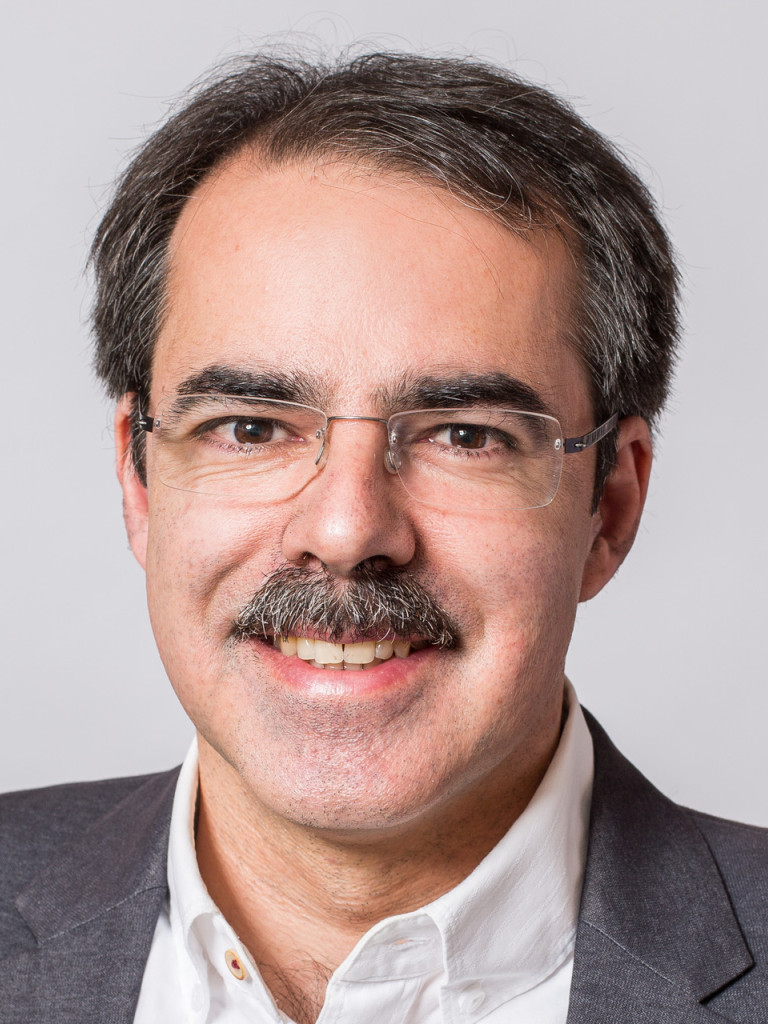
\includegraphics[width=\linewidth]{figures/hintermueller.jpg}
    \captionof*{figure}{\tiny M. Hinterm\"uller}
  \end{minipage}}%
  \hfill
  \begin{minipage}[b]{0.46\textwidth}
    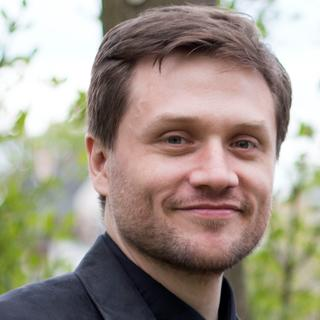
\includegraphics[width=\linewidth]{figures/rautenberg.jpg}
    \captionof*{figure}{\tiny C.N. Rautenberg}
  \end{minipage}
\end{figure}
 \begin{minipage}[b]{0.5\textwidth}
    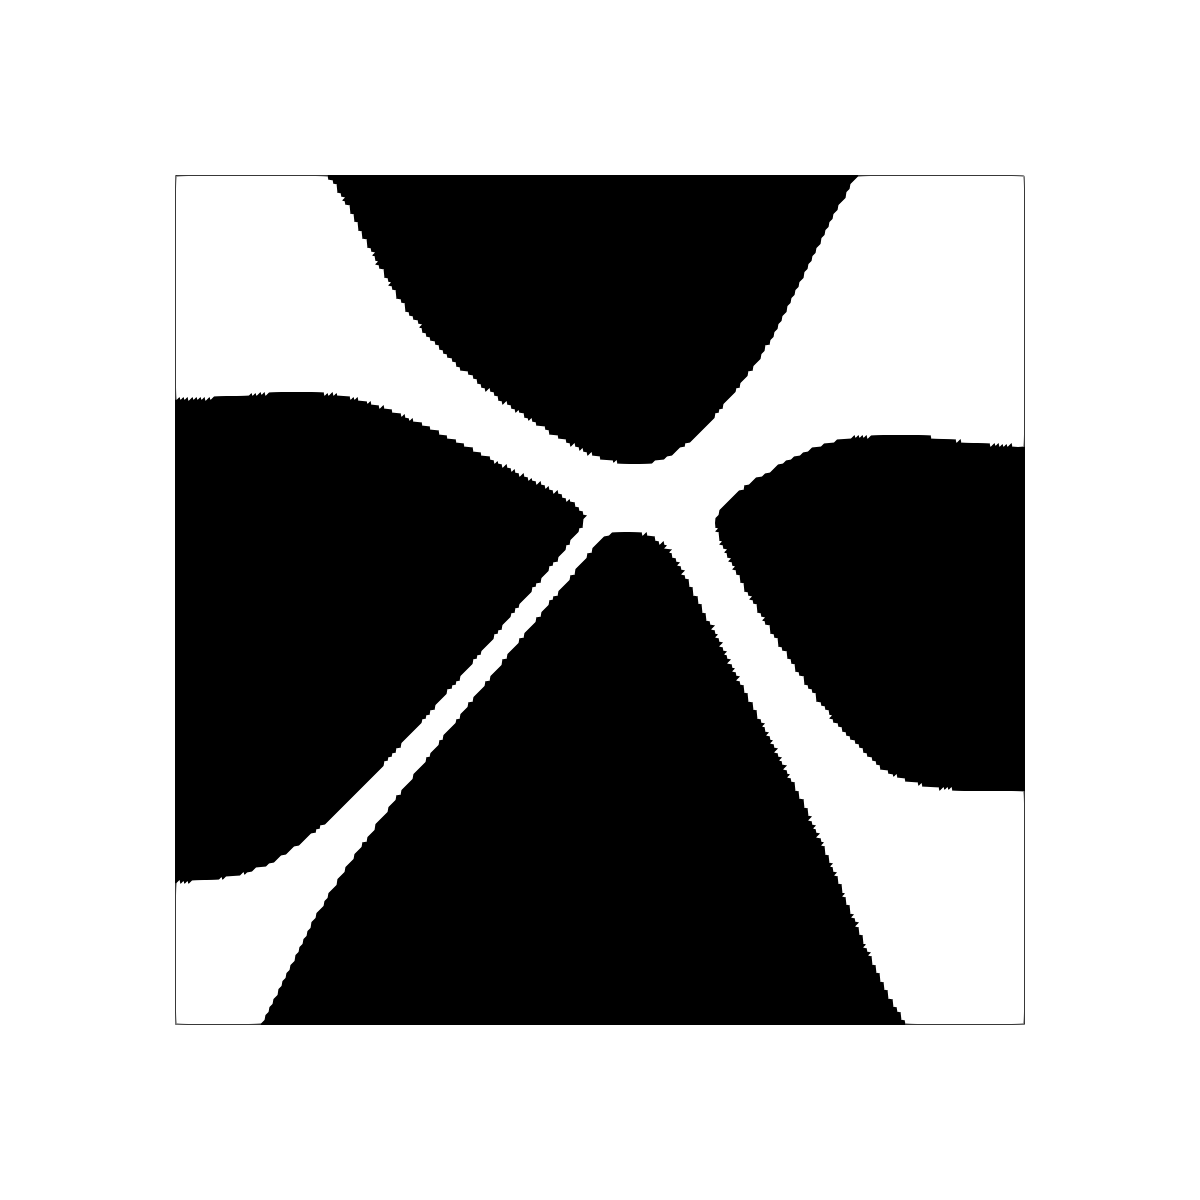
\includegraphics[width=\linewidth]{figures/global_feasible_active_set.png}
    \captionof*{figure}{\tiny Black: $|\nabla u| = \phi$.}
  \end{minipage}%
%  \hfill
%  \begin{minipage}[b]{0.6\textwidth}
    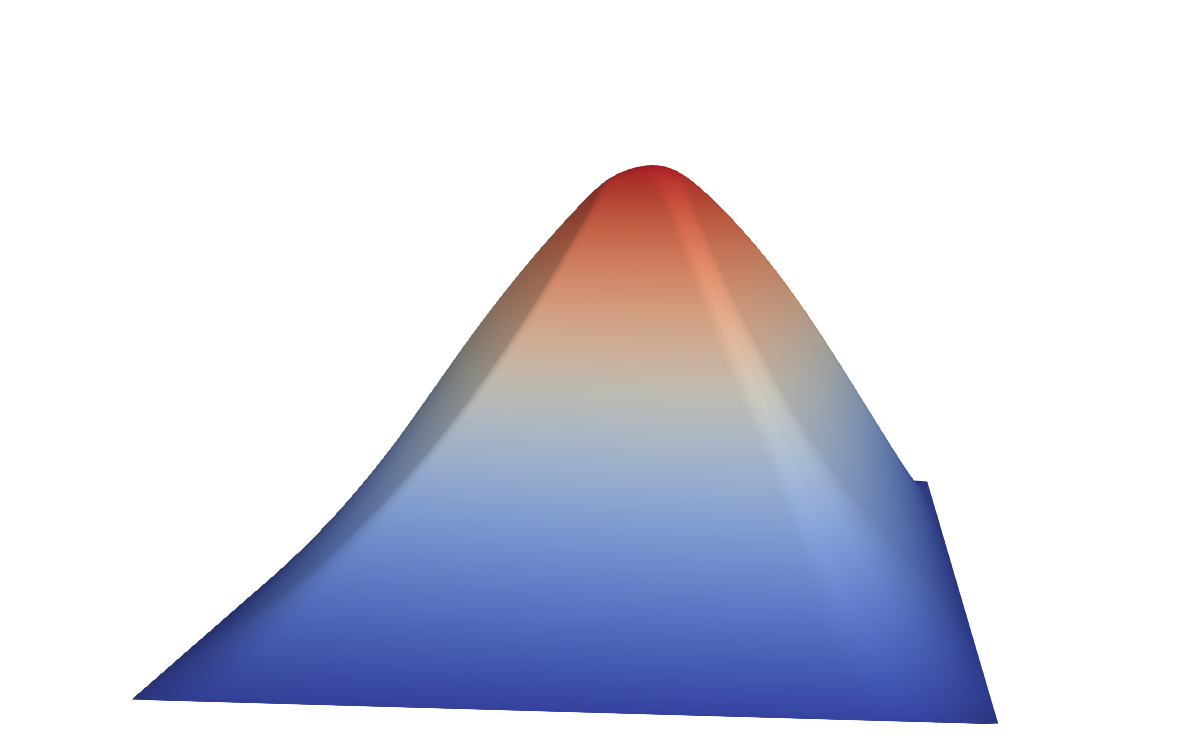
\includegraphics[width=0.8\linewidth]{figures/gradient_constraint_u.png}
%    \captionof*{figure}{\tiny \hspace{28ex} State $u$ for $p=2$}
%  \end{minipage}
%\begin{figure}
%	\centering
%	\begin{tikzpicture}
%		\node at (-5,0) {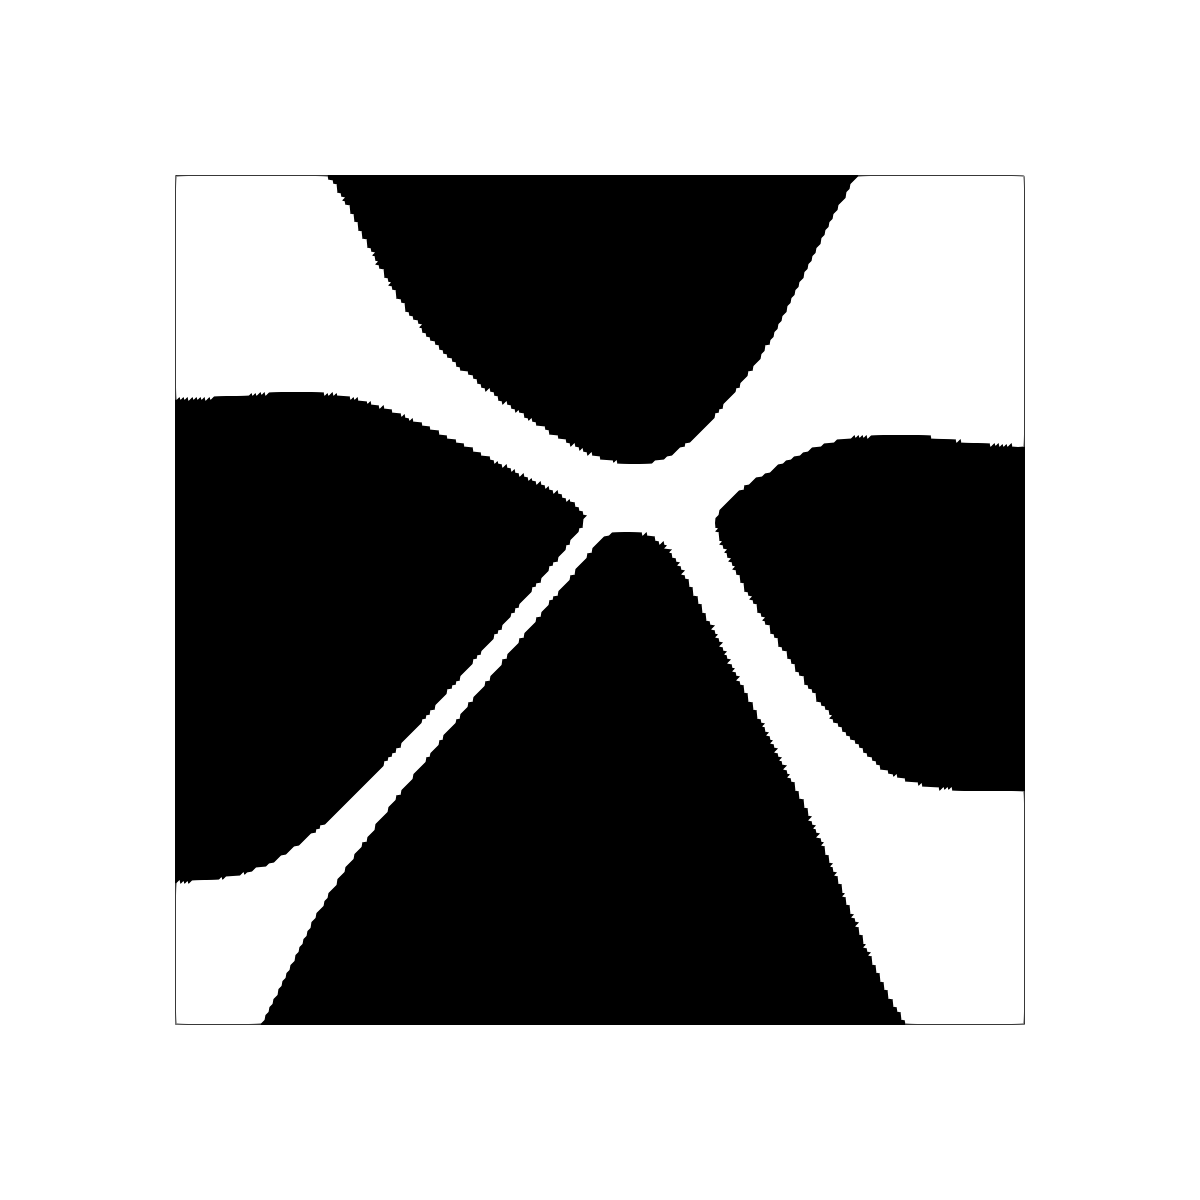
\includegraphics[height=1in]{figures/global_feasible_active_set.png}};\hspace{10ex}
%    \end{tikzpicture}\vspace{-8ex}
%	\begin{tikzpicture}
%		\node at (-2,-1) {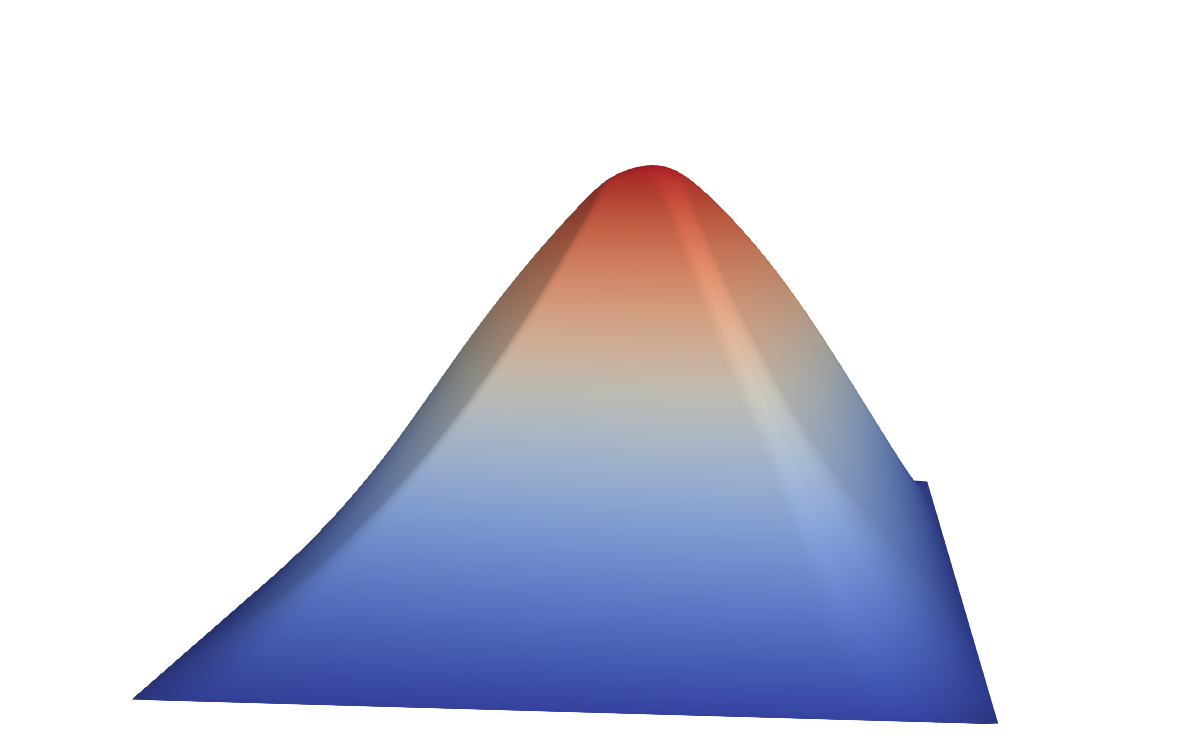
\includegraphics[height=1.25in]{figures/gradient_constraint_u.png}};
%    \end{tikzpicture}
%%\end{figure}
%  \end{minipage}
\end{minipage}
\end{frame}

%\begin{frame}{Further Examples}
%\begin{figure}
%  \centering
%  \begin{subfigure}[b]{0.19\textwidth}
%    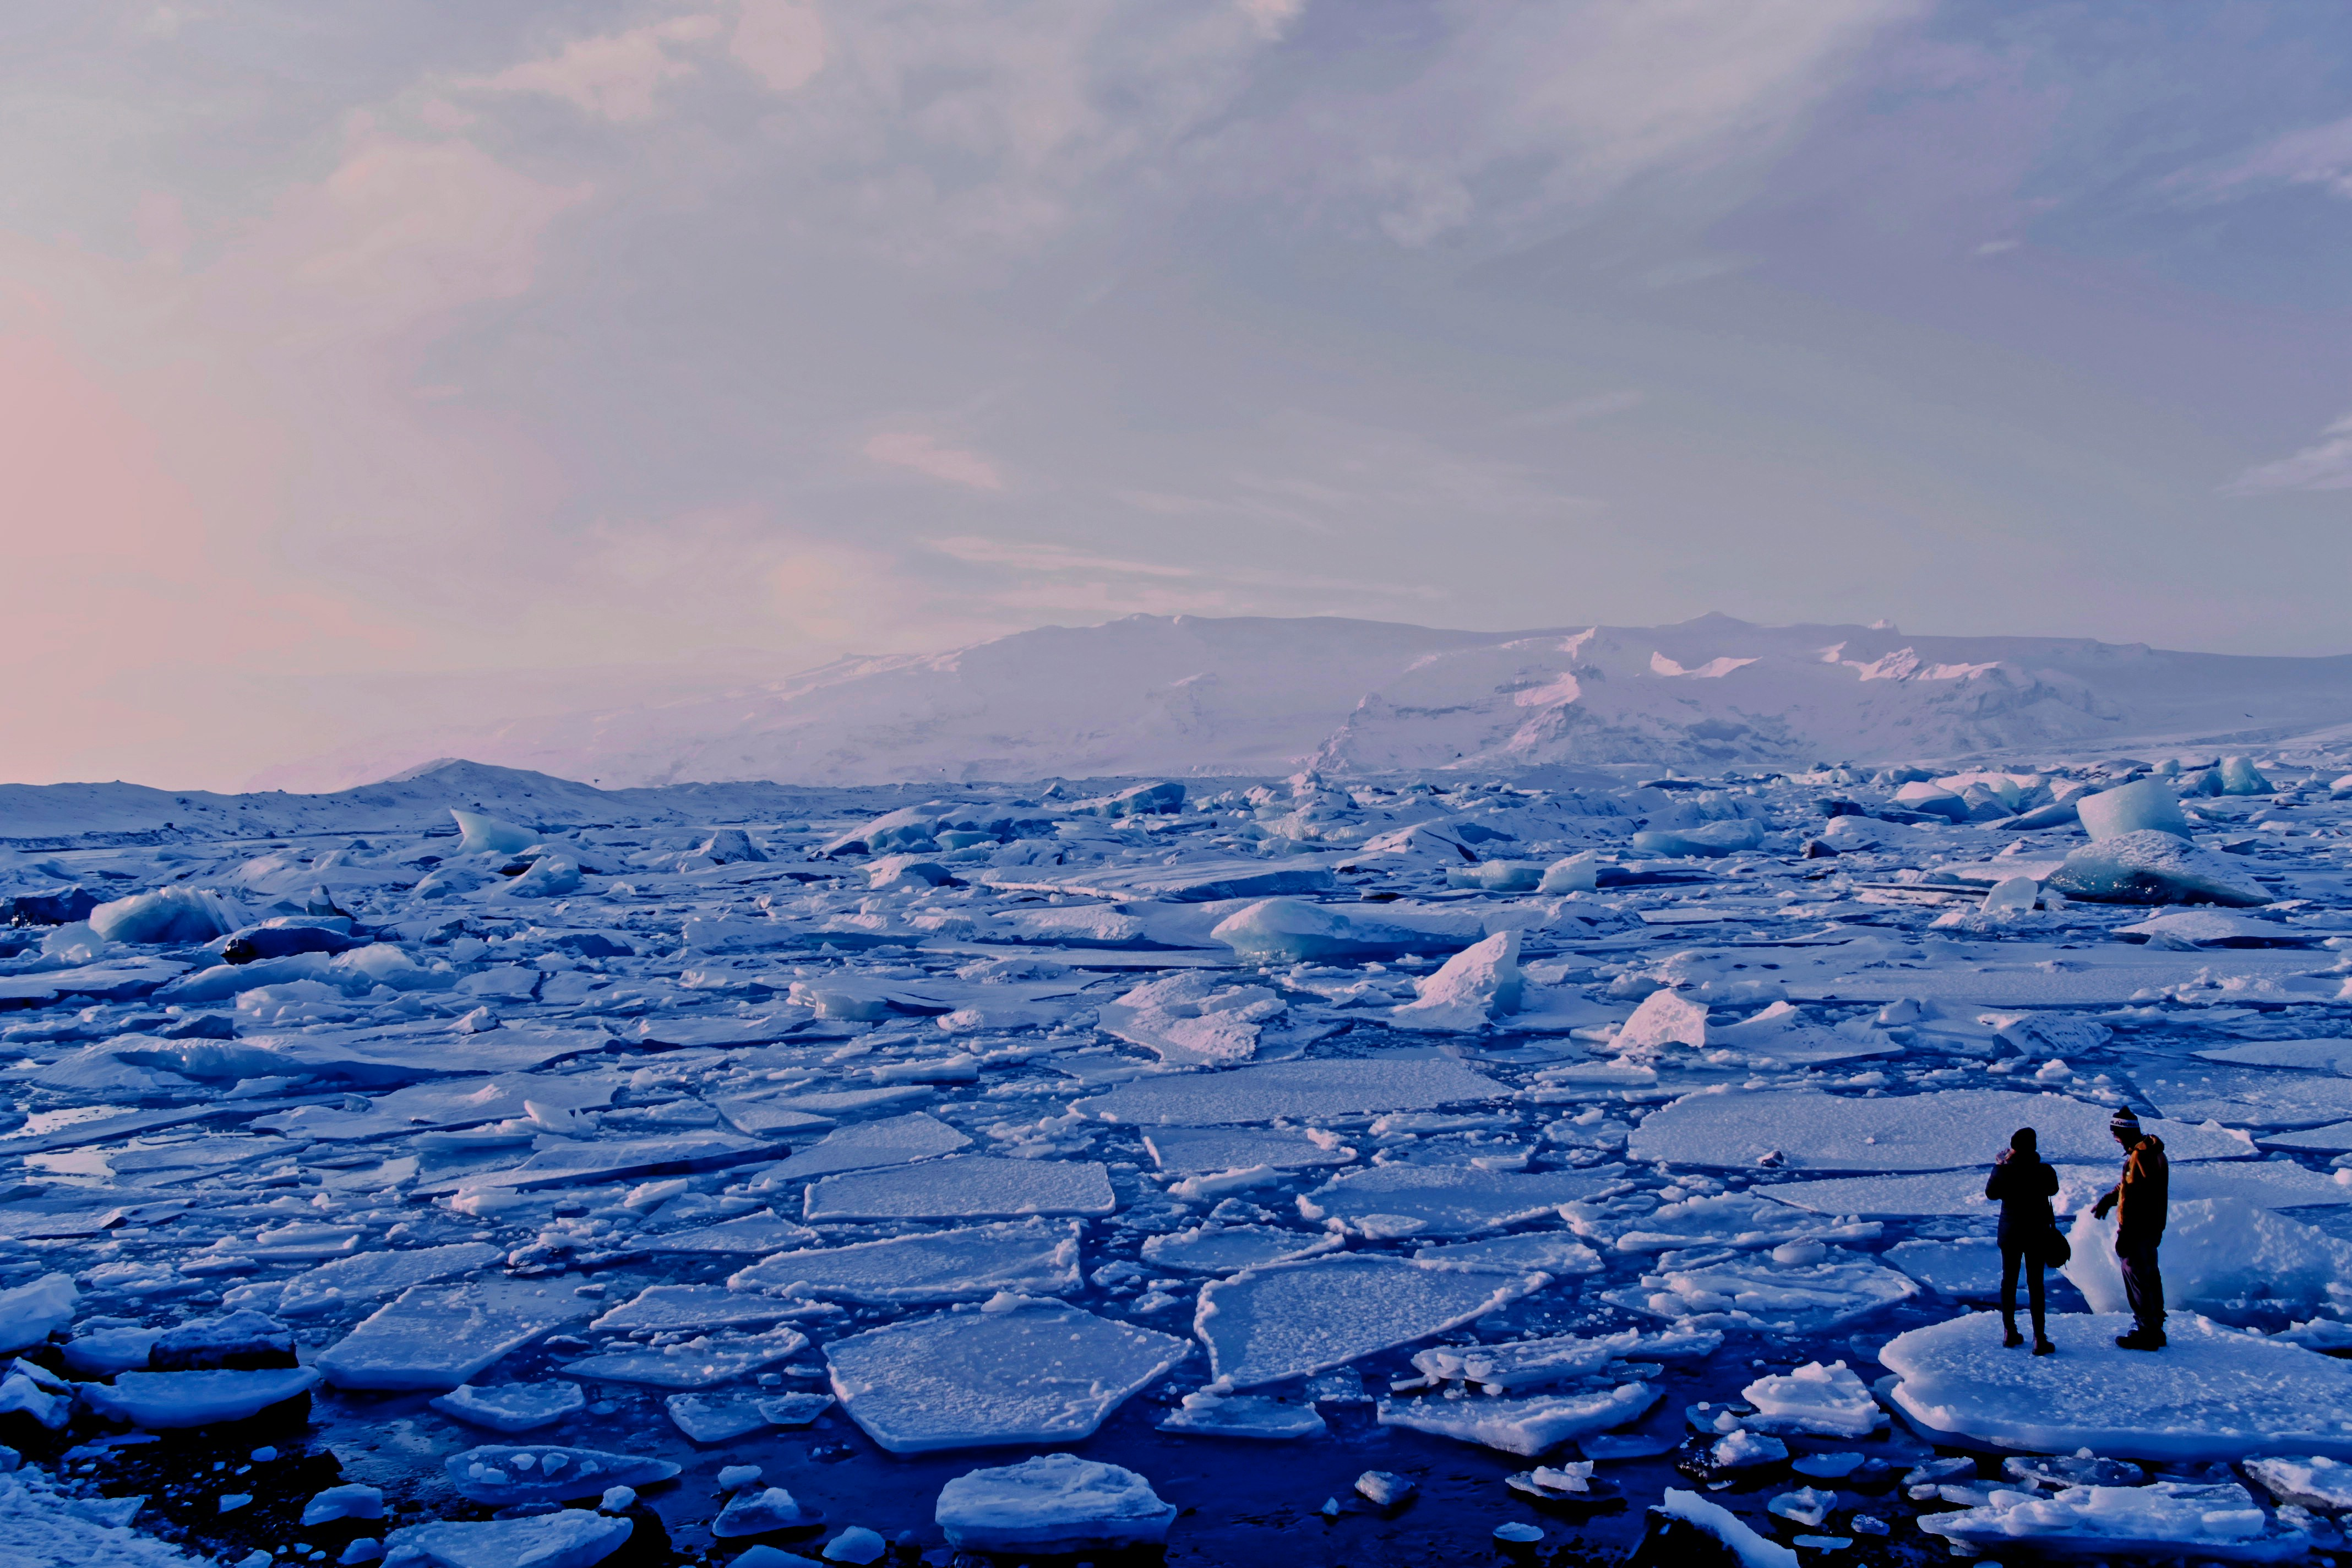
\includegraphics[width=\linewidth]{figures/ice.jpg}
%    \caption{Stefan Problem}
%  \end{subfigure}
%  \hfill
%  \begin{subfigure}[b]{0.19\textwidth}
%    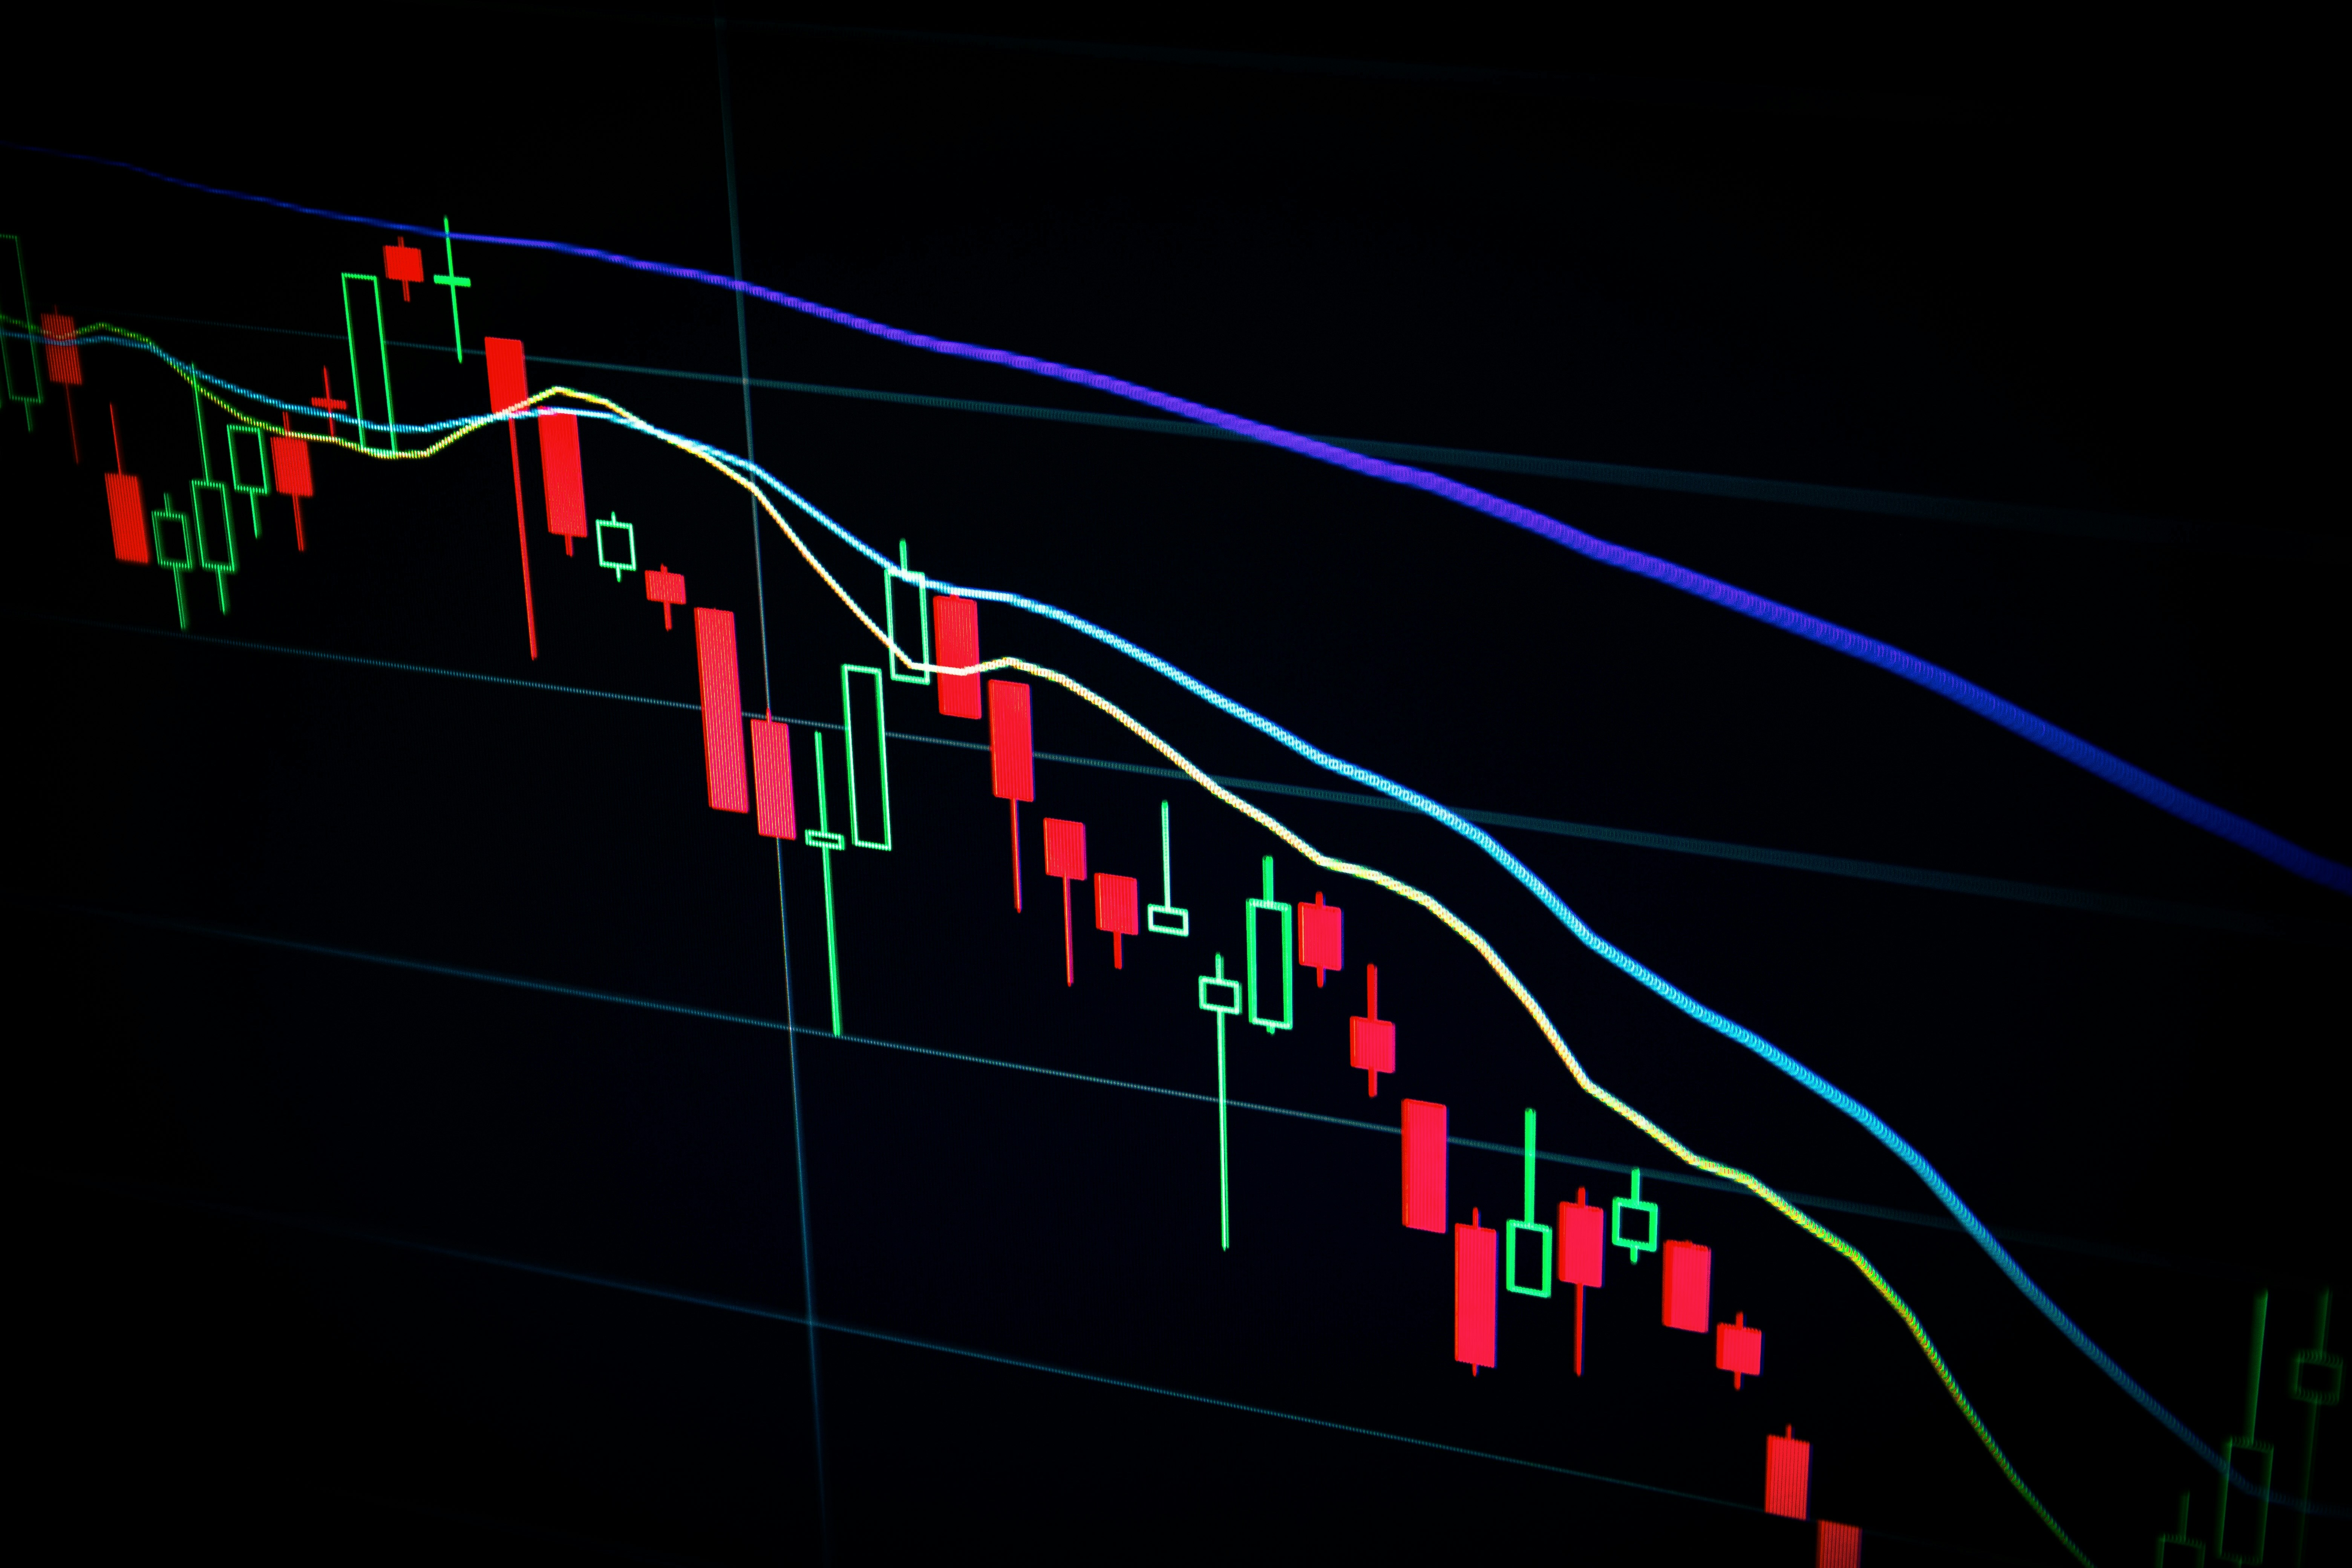
\includegraphics[width=\linewidth]{figures/stocks.jpg}
%    \caption{Option Pricing}
%  \end{subfigure}
%  \hfill
%  \begin{subfigure}[b]{0.19\textwidth}
%    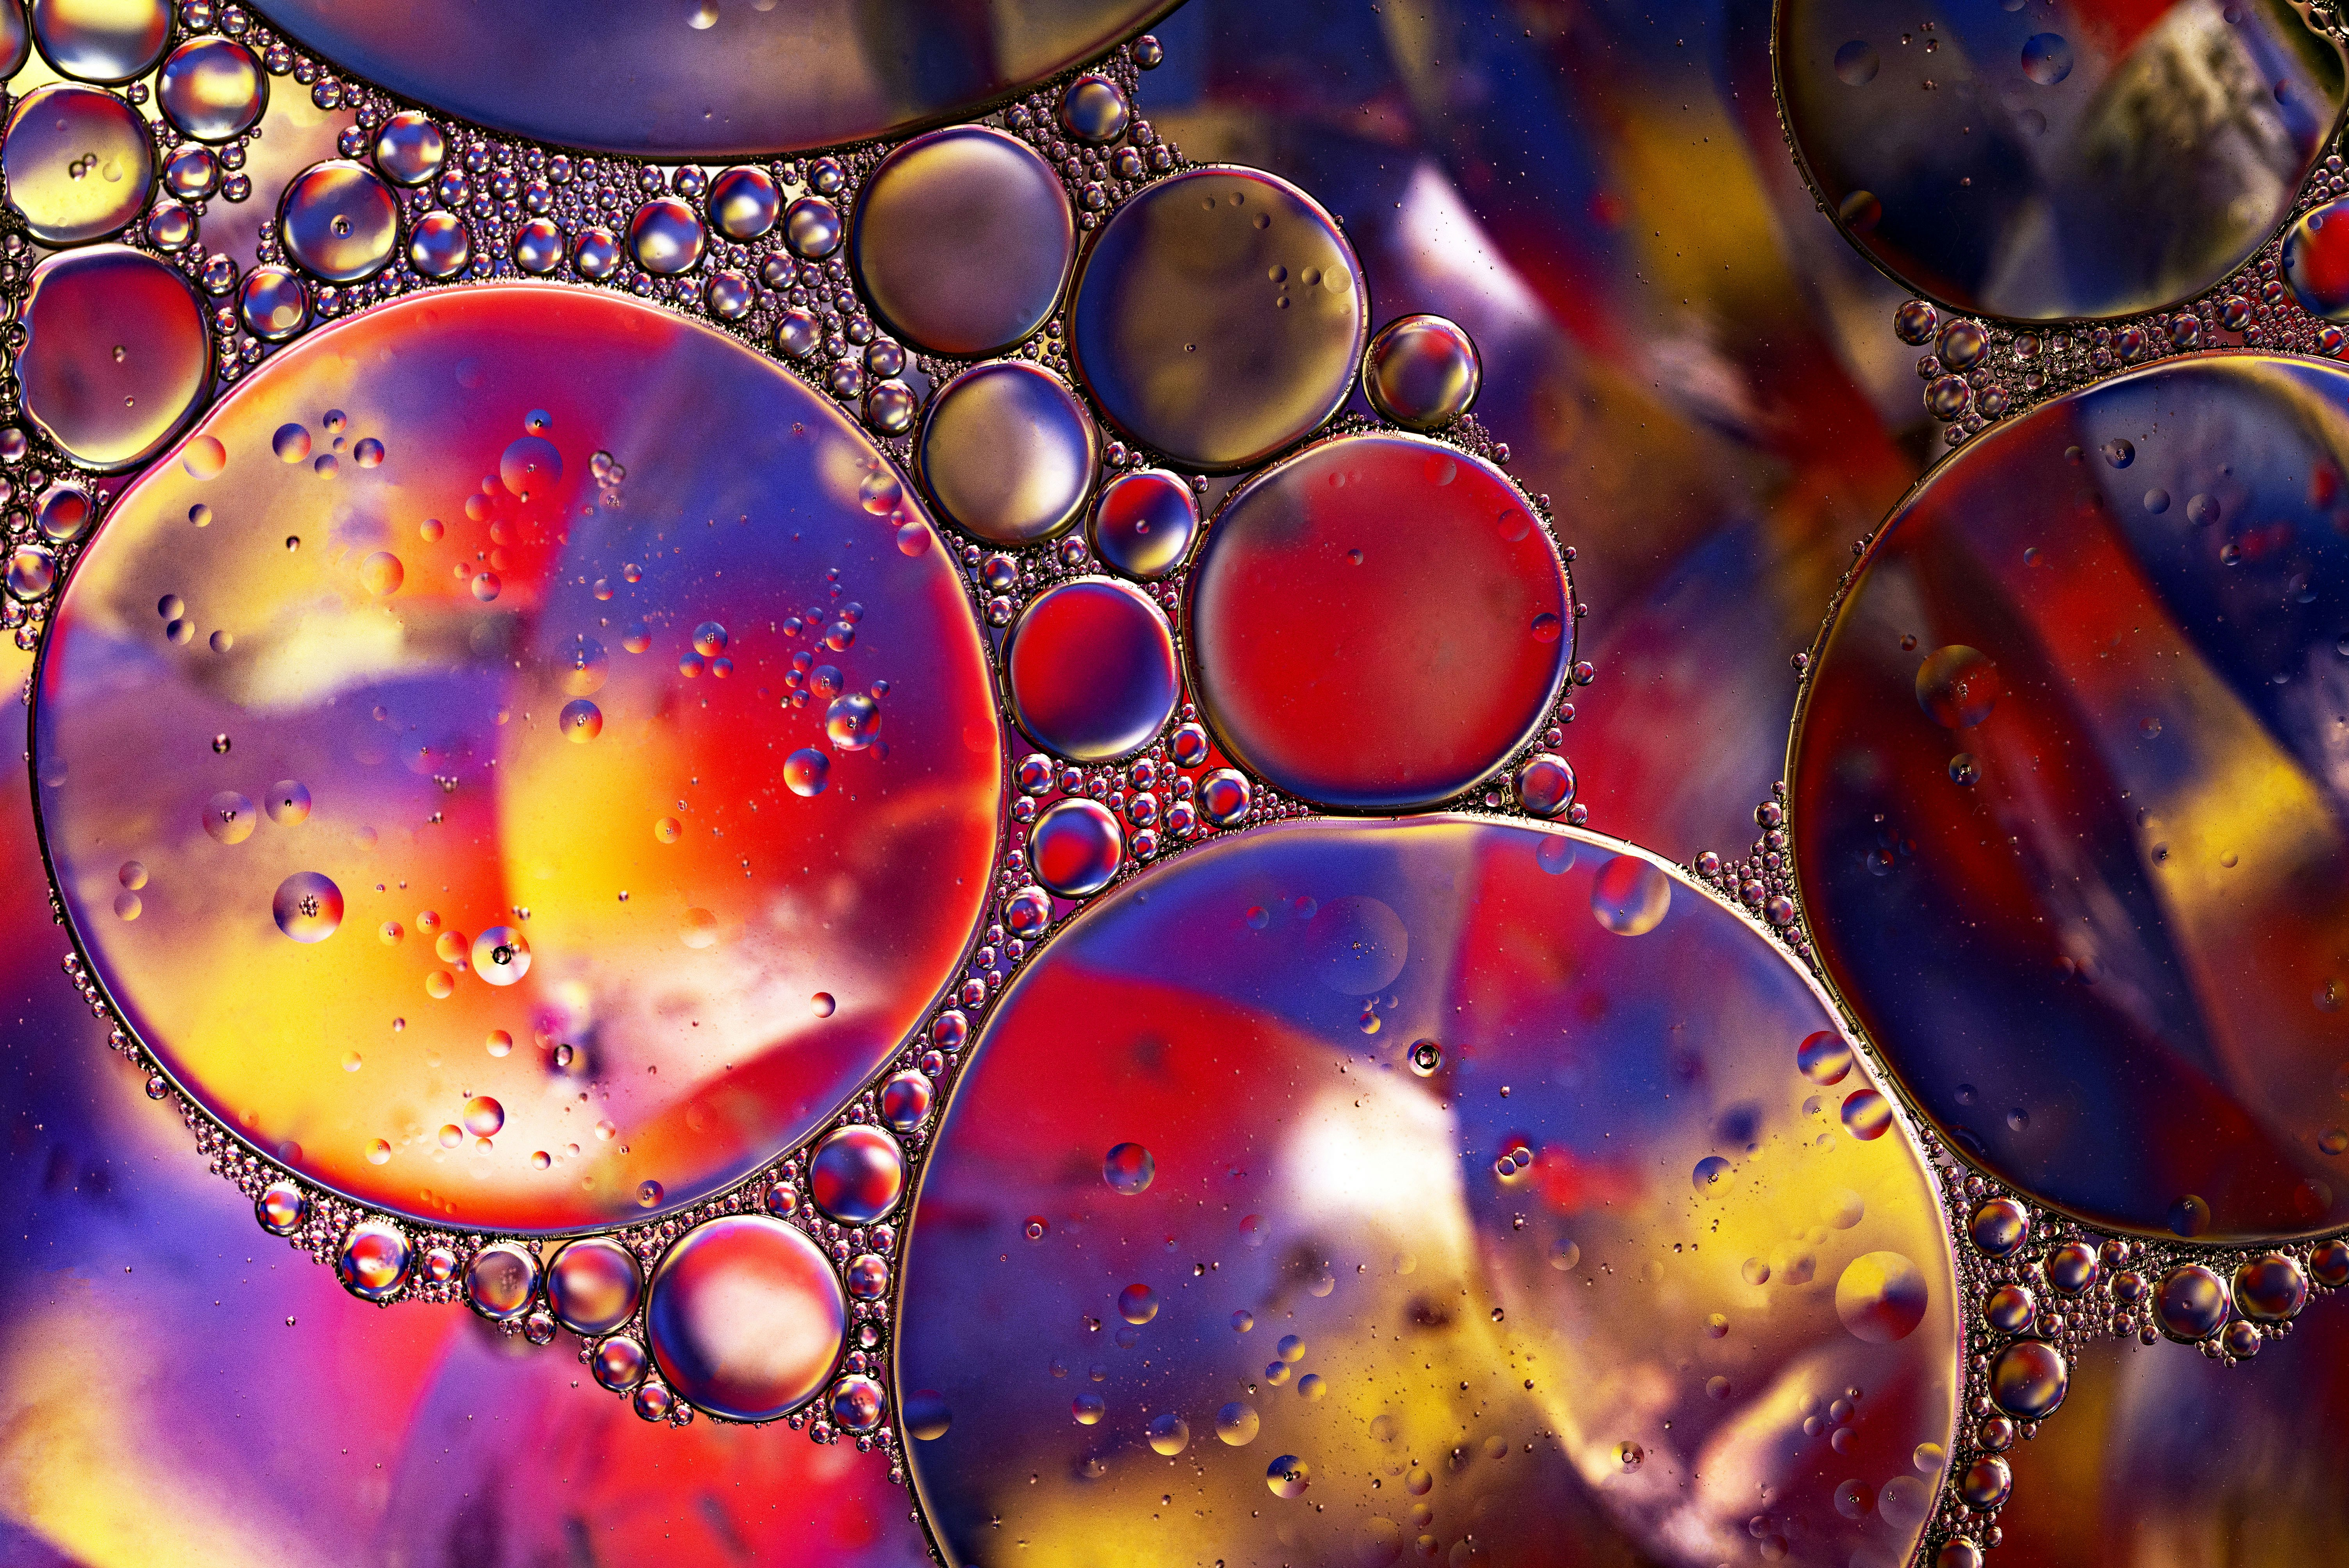
\includegraphics[width=\linewidth]{figures/water-oil-2.jpg}
%    \caption{Phase Transition}
%  \end{subfigure}\\
%%  \hfill
%  \begin{subfigure}[b]{0.19\textwidth}
%    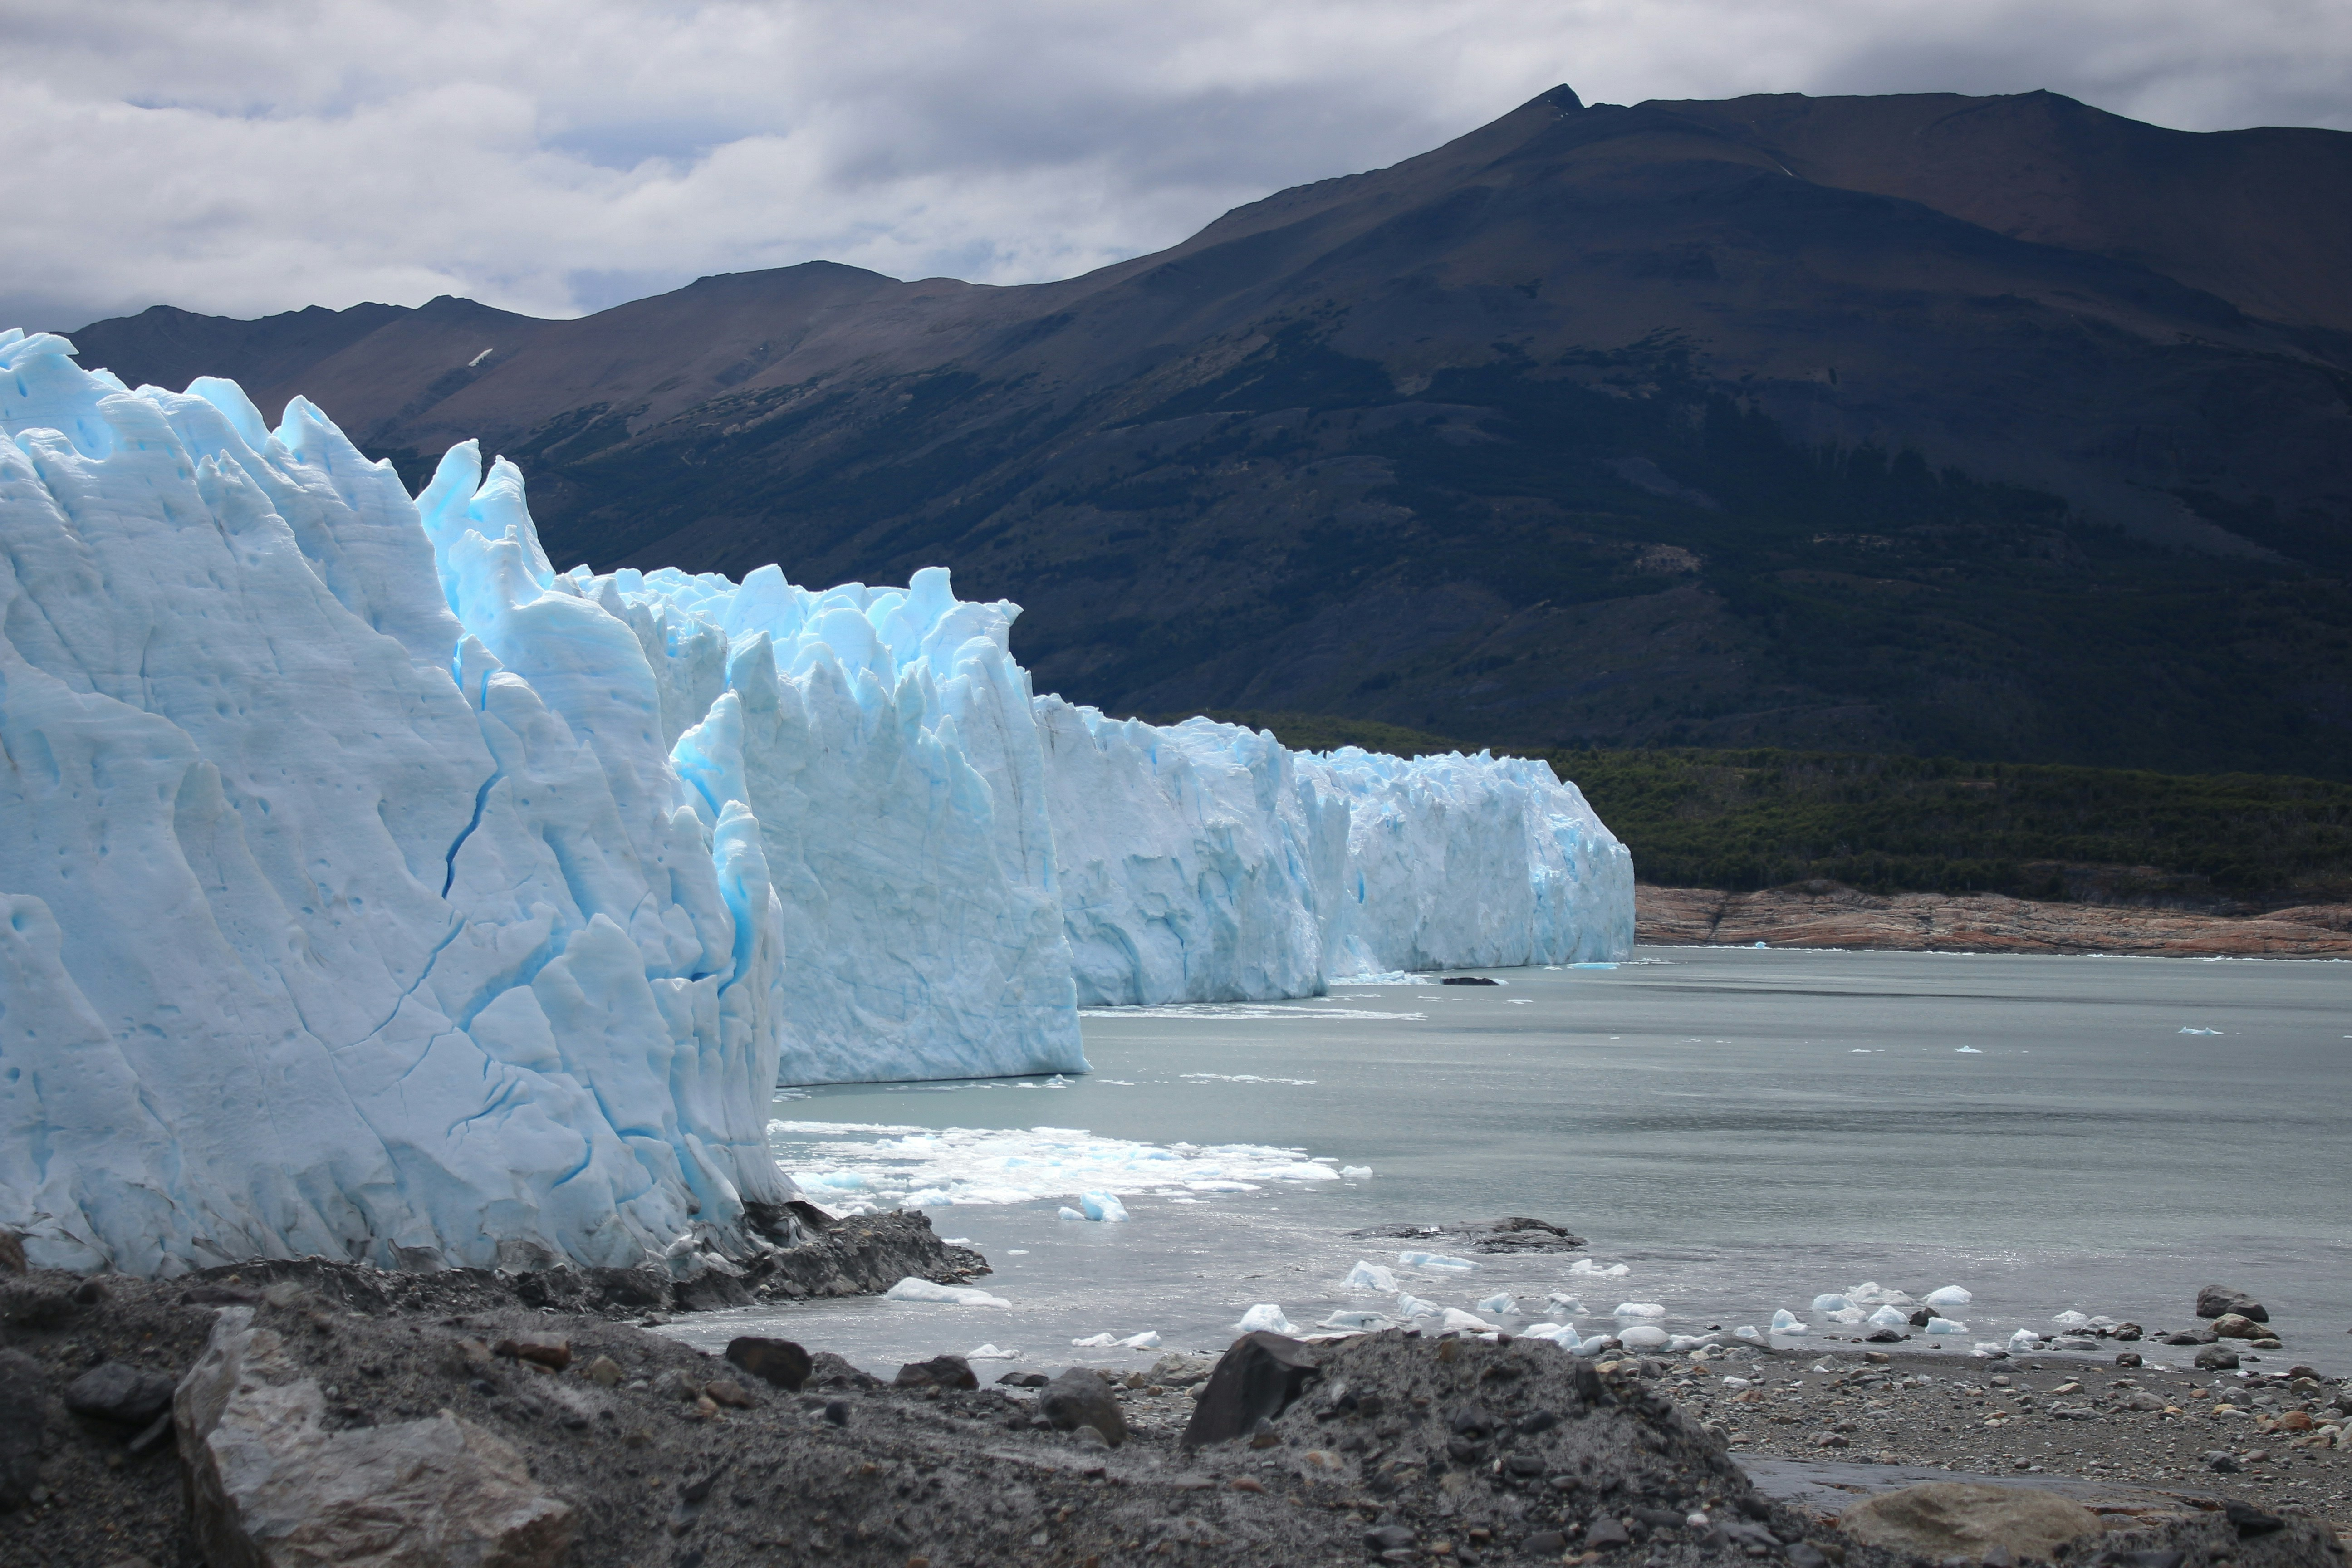
\includegraphics[width=\linewidth]{figures/glacier.jpg}
%    \caption{Ice Sheet Models}
%  \end{subfigure}
%\hspace{7em}	
%%  \hfill
%  \begin{subfigure}[b]{0.19\textwidth}
%    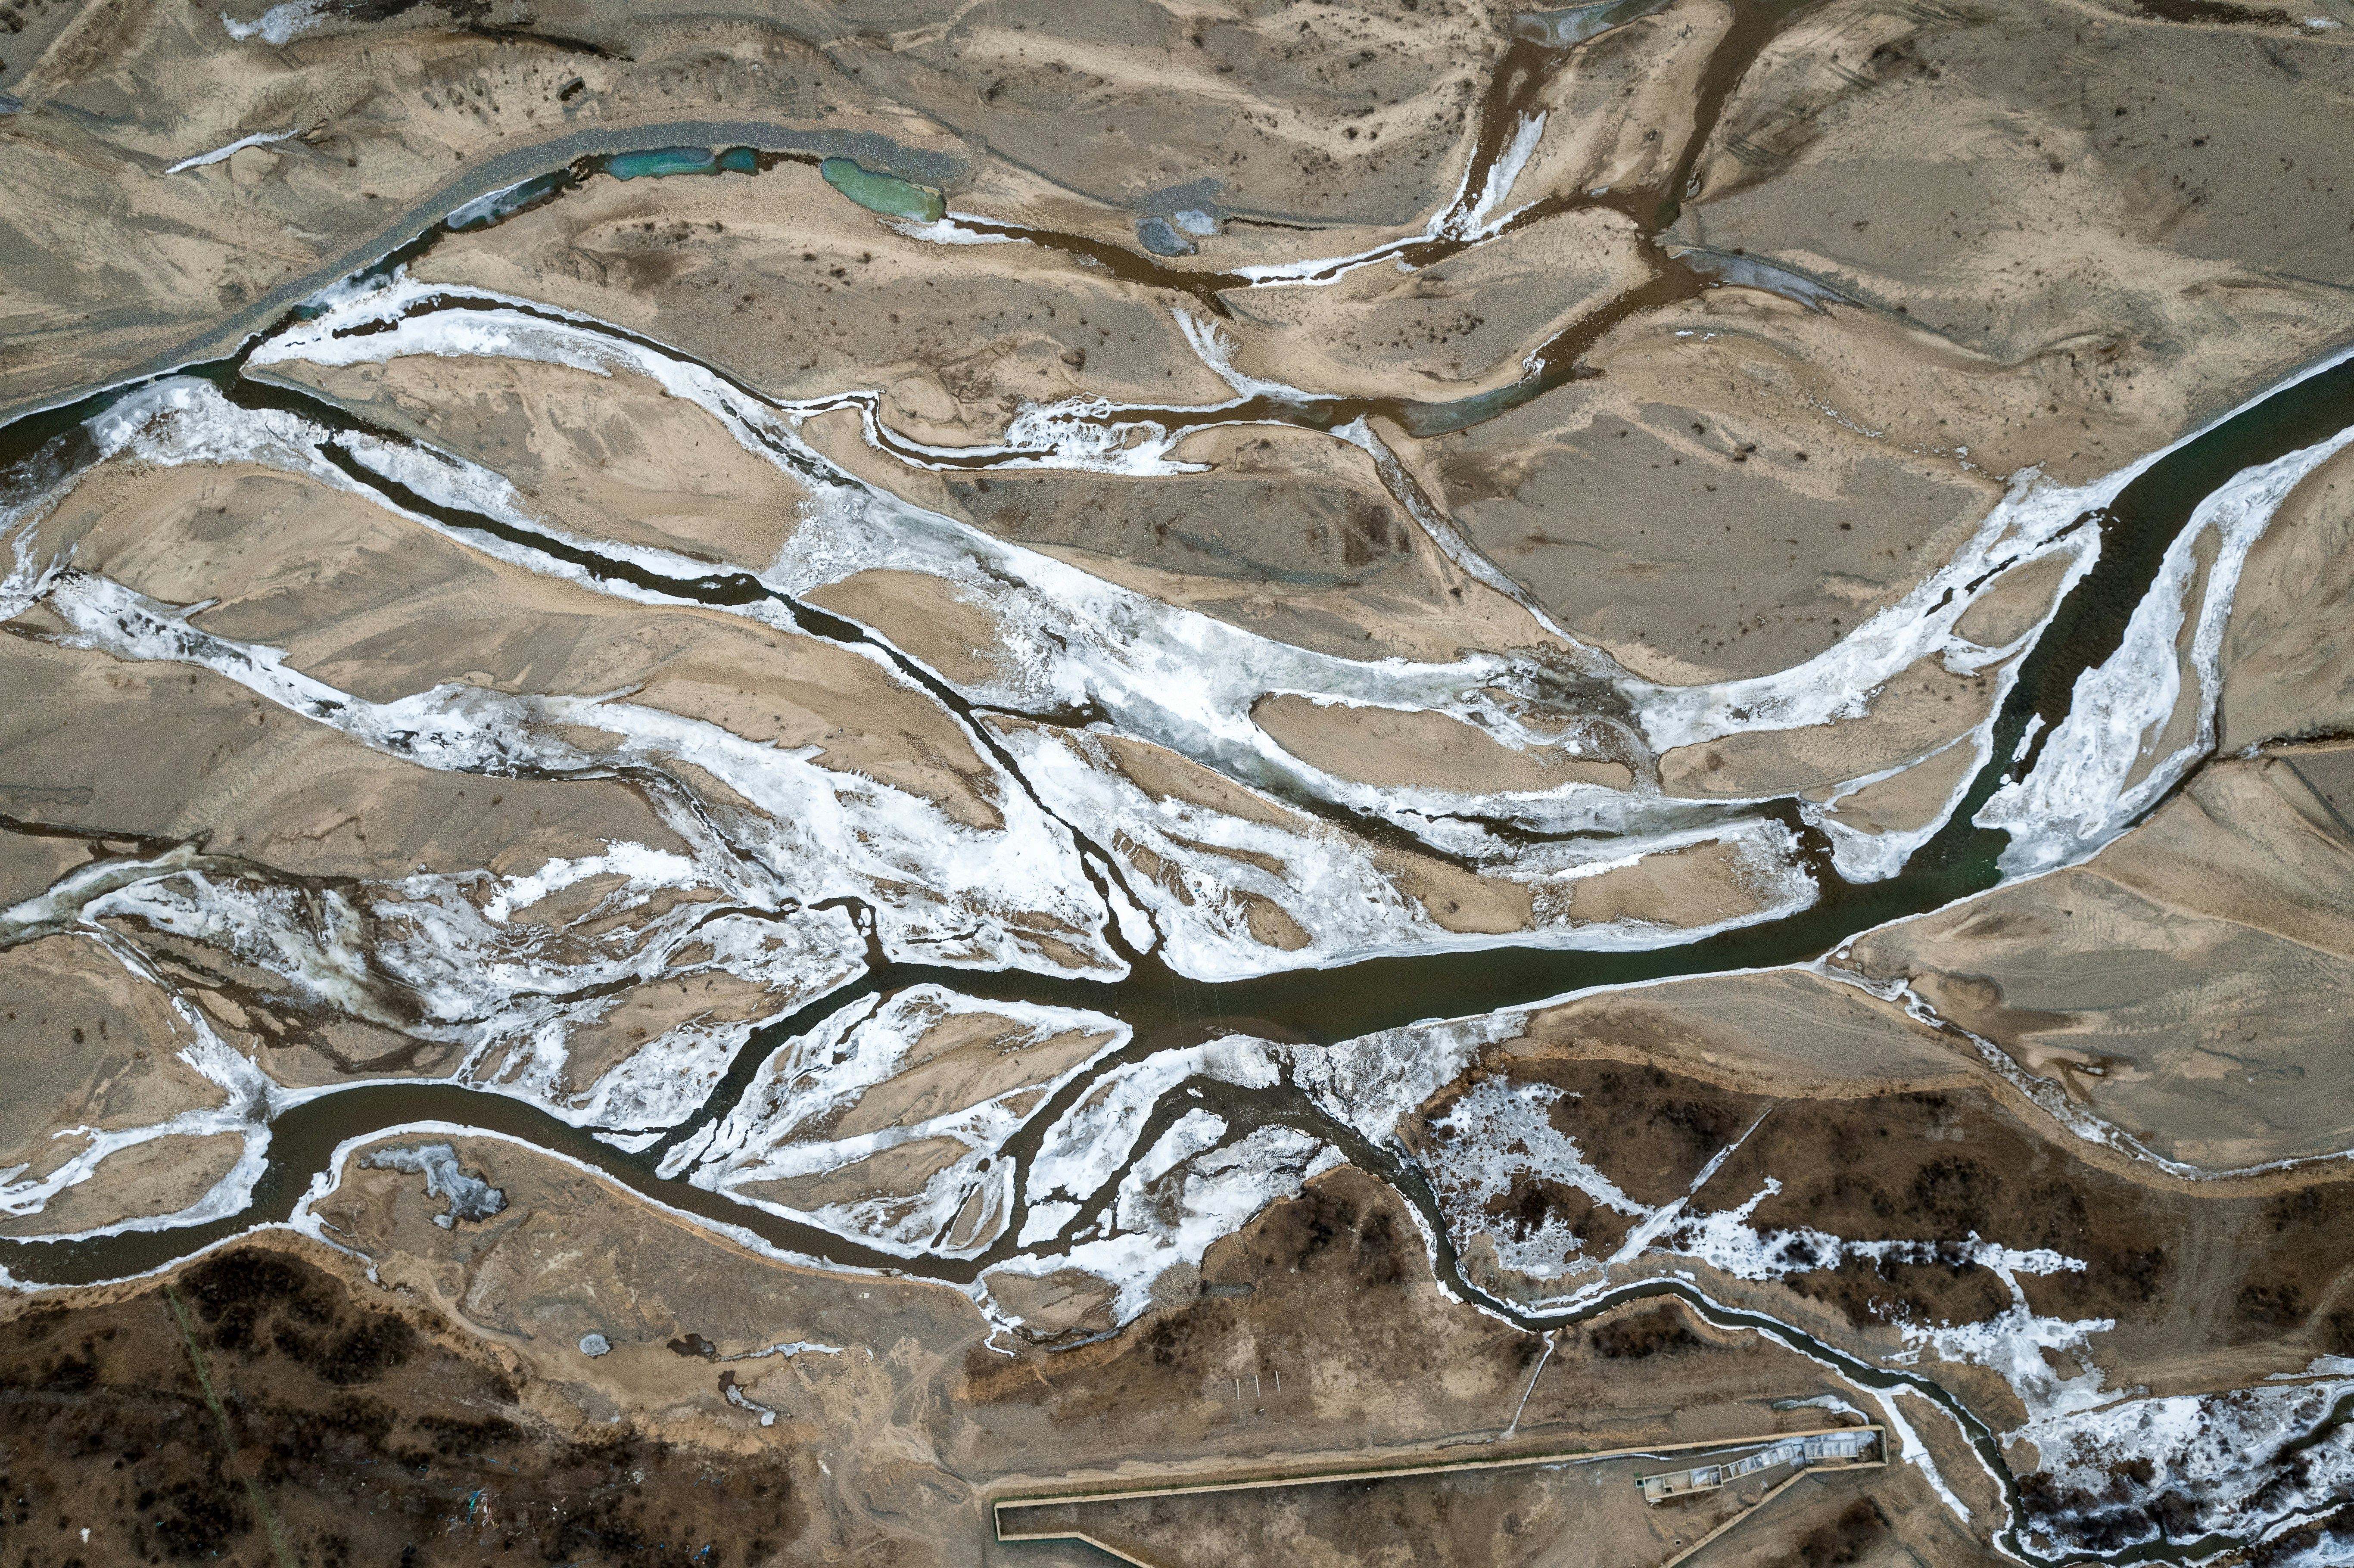
\includegraphics[width=\linewidth]{figures/rivers.jpg}
%    \caption{Diffusive Waves}
%  \end{subfigure}
%\end{figure}
% \visible<1->{\begin{beamercolorbox}[rounded=true, shadow=true, wd=\textwidth]{block title}
% \centering Each one of these applications can be formulated as a variational inequality with nontrivial pointwise inequality constraints on the state!
% \end{beamercolorbox}
% }
%\end{frame}

%\subsection{Examples}\label{sec:examples}
%\begin{frame}{Examples of Variational Inequalities}
%    \begin{enumerate}
%%        \item Signorini problem
%%        \item Stefan problem
%%        \item Black-Scholes
%%        \item Multiphase phase transition
%%        \item Elastoplastic torsion
%%        \item Ice sheet
%        \item Diffusive wave equation
%    \end{enumerate}
%\end{frame}

%\begin{frame}{Elliptic Variational Inequalities}
%        \begin{enumerate}
%        \item A slight twist on Dirichlet's principle
%            \begin{enumerate}
%                \item Conic constraint ($u \ge 0$)
%                \item Follow Dirichlet above for derivation
%            \end{enumerate}
%        \item A second variational inequality: An obstacle problem
%        \item A brief history of variational inequalities (of the first kind)
%        \item The Lions-Stampacchia theorem
%        \item Mignot's theorem
%            \begin{enumerate}
%                \item 
%            \end{enumerate}
%    \end{enumerate}
%\end{frame}

\begin{frame}\frametitle{The Obstacle Problem}
\only<1-3>{
%\begin{minipage}{0.45\linewidth}
\begin{beamercolorbox}[rounded=true, shadow=true, wd=\textwidth]{block body}
 \visible<1->{A deceptively simple twist on Dirichlet's principle...\medskip
 
 }\visible<2->{
 We seek a minimizer $u$ of the total energy functional:
 \begin{equation*}
 	E(v)
 	=
 	\frac{1}{2}
 	\int_\Omega |\nabla v|^2 \dd x
 	-
 	\int_\Omega f v\dd x
 	\,,
 \end{equation*}
 
  }\visible<3->{
 over the \textbf{closed convex set} defined by  
 \[
 K = \{ v \in H^1(\Omega) \mid  v \ge \varphi \text{~a.e. }  v|_{\Gamma} = g \}
 \] 
 with $\varphi \in H^1(\Omega)$, $(\varphi - g)|_{\Gamma} \ge 0$.
} 
\end{beamercolorbox}}
%\end{minipage}}%
%\only<4->{
%\begin{minipage}{0.45\linewidth}
%\begin{beamercolorbox}[rounded=true, shadow=true, wd=\textwidth]{block title}
% \visible<1->{A deceptively simple twist on Dirichlet's principle...\medskip
% 
% }\visible<2->{
% We seek a minimizer $u$ of the total energy functional:
% \begin{equation*}
% 	E(v)
% 	=
% 	\frac{1}{2}
% 	\int_\Omega |\nabla v|^2 \dd x
% 	-
% 	\int_\Omega f v\dd x
% 	\,,
% \end{equation*}
% 
%  }\visible<3->{
% over the \textbf{closed convex set} defined by  
% \[
% K = \{ v \in H^1(\Omega) \mid  v \ge \varphi \text{~a.e. }  v|_{\Gamma} = g \}
% \] 
% with $\varphi \in H^1(\Omega)$, $(g - \varphi)|_{\Gamma} \ge 0$.
%} 
%\end{beamercolorbox}
%\end{minipage}}%
%\only<4->{%
%\begin{minipage}{0.55\linewidth}
%%\hspace{-4ex}
%\begin{beamercolorbox}[rounded=true, shadow=true, wd=\textwidth]{block body}
%Existence of solutions:
%\begin{itemize}
%\item \visible<5->{The analysis follows Dirichlet's principle.}
%\item \visible<6->{\alert{New}: We must view $E : K \subsetneq H^1(\Omega) \to \overline{\mathbb R}$}
%\item \visible<7->{Is $K$ weakly sequentially compact? \alert{No.}}
%\item \visible<8->{We  \alert{can}, however, show that $K \cap N_0$ is!}
%\end{itemize}
%\end{beamercolorbox}
%\end{minipage}
%}
\end{frame}

%\begin{frame}\frametitle{The Obstacle Problem}
%\only<1-3>{
%\begin{minipage}{0.45\linewidth}
%\begin{beamercolorbox}[rounded=true, shadow=true, wd=\textwidth]{block body}
% \visible<1->{A deceptively simple twist on Dirichlet's principle...\medskip
% 
% }\visible<2->{
% We seek a minimizer $u$ of the total energy functional:
% \begin{equation*}
% 	E(v)
% 	=
% 	\frac{1}{2}
% 	\int_\Omega |\nabla v|^2 \dd x
% 	-
% 	\int_\Omega f v\dd x
% 	\,,
% \end{equation*}
% 
%  }\visible<3->{
% over the \textbf{closed convex set} defined by  
% \[
% K = \{ v \in H^1(\Omega) \mid  v \ge \varphi \text{~a.e. }  v|_{\Gamma} = g \}
% \] 
% with $\varphi \in H^1(\Omega)$, $(\varphi - g)|_{\Gamma} \ge 0$.
%} 
%\end{beamercolorbox}
%\end{minipage}}%
%\only<4->{
%\begin{minipage}{0.45\linewidth}
%\begin{beamercolorbox}[rounded=true, shadow=true, wd=\textwidth]{block title}
% \visible<1->{A deceptively simple twist on Dirichlet's principle...\medskip
% 
% }\visible<2->{
% We seek a minimizer $u$ of the total energy functional:
% \begin{equation*}
% 	E(v)
% 	=
% 	\frac{1}{2}
% 	\int_\Omega |\nabla v|^2 \dd x
% 	-
% 	\int_\Omega f v\dd x
% 	\,,
% \end{equation*}
% 
%  }\visible<3->{
% over the \textbf{closed convex set} defined by  
% \[
% K = \{ v \in H^1(\Omega) \mid  v \ge \varphi \text{~a.e. }  v|_{\Gamma} = g \}
% \] 
% with $\varphi \in H^1(\Omega)$, $(g - \varphi)|_{\Gamma} \ge 0$.
%} 
%\end{beamercolorbox}
%\end{minipage}}%
%\only<4->{%
%\begin{minipage}{0.55\linewidth}
%%\hspace{-4ex}
%\begin{beamercolorbox}[rounded=true, shadow=true, wd=\textwidth]{block body}
%Existence of solutions:
%\begin{itemize}
%\item \visible<5->{The analysis follows Dirichlet's principle.}
%\item \visible<6->{\alert{New}: We must view $E : K \subsetneq H^1(\Omega) \to \overline{\mathbb R}$}
%\item \visible<7->{Is $K$ weakly sequentially compact? \alert{No.}}
%\item \visible<8->{We  \alert{can}, however, show that $K \cap N_0$ is!}
%\end{itemize}
%\end{beamercolorbox}
%\end{minipage}}
%\end{frame}

%\begin{frame}\frametitle{Direct Method: Extra Step}
%\begin{beamercolorbox}[rounded=true, shadow=true, wd=\textwidth]{block body}\scriptsize
%\visible<1->{$K \ne \emptyset$ : Construct a feasible point using Dirichlet's principle and the Maximum Principle.\bigskip
%
%}\visible<2->{$K$ is convex: $v,w \in K$, $\lambda \in [0,1]$ $\Rightarrow$ $\lambda v + (1-\lambda) w \ge \lambda \varphi + (1-\lambda) \varphi = \varphi$, same as before for boundary data.\bigskip
%
%}\visible<3->{$K$ is closed:  \visible<4->{Take $\left\{v_k\right\} \subset K$ such that $v_k \to v$ (strongly) in $H^1(\Omega)$. }
%\begin{itemize}
%\item \visible<5->{Clearly, $v_k-\varphi \to v-\varphi$ (strongly) in $L^2(\Omega)$.} 
%\item \visible<6->{For any $w \in L^2(\Omega)$ : $w \ge 0$, we have $(v_k-\varphi,w) \ge 0$. Hence, $(v-\varphi,w) \ge 0$.}
%\item \visible<7->{Since $w$ is arbitrary, $v \ge \phi$ a.e.\ in $\Omega$.}
%%\item \visible<5->{$H^1(\Omega) \hookrightarrow L^1(\Omega)$ continuously, hence $v_k \to v$ (strongly) in $L^1(\Omega)$.} 
%%\item \visible<6->{$L^1(\Omega)$ convergence implies  $\exists \left\{v_{k_l}\right\} \subset \left\{v_k\right\}$ such that $v_{k_l} \to v$ pointwise a.e.}
%%\item \visible<7->{For all $k$: $v_{k} \ge \varphi$ a.e.\ (by definition), clearly for $k_l$ as well. Hence, $v \ge \varphi$.}
%\item \visible<8->{The trace is continuous, hence $g = v_{k}|_{\Gamma} \to v|_{\Gamma} = g$.}
%\end{itemize}}\bigskip
%
%\visible<9->{$K$ is \alert{weakly closed}: Closed convex sets in locally convex TVS are the intersections of all closed half spaces containing them, thus weakly closed ($\Rightarrow$ \alert{weakly sequentially closed}).\bigskip
%
%}\visible<10->{
%If $\{v_k\} \subset K \cap N_0$ is a minimizing sequence, then its weak accumulation points lie in $K$!
%}
%\end{beamercolorbox}
%\end{frame}

\begin{frame}\frametitle{The Obstacle Problem}
\begin{beamercolorbox}[rounded=true, shadow=true, wd=\textwidth]{block body}
Same arguments as in DP lead to a variational inequality as an optimality condition:\medskip

Find $u \in K$ such that
 \[
 (\nabla u, \nabla [v-u])_{L^2} \ge  (f,v-u)_{L^2} \quad \forall v \in K.
 \]
 
 \visible<2->{
 $K$ is not a balanced set $\Rightarrow$ no clever test functions $v \in K$ that turn this into an \alert{equation}.\medskip
 
 }
% \visible<3->{
%Observation 1: $f$ can have less regularity, i.e., $f \in (H^1(\Omega))^*$.\medskip
 
% }
 \visible<3->{
The proofs for existence and derivation of the VI carry over to more \alert{general (smooth) objectives} $J$ and \alert{closed convex sets} $K$ in \alert{reflexive Banach spaces}.\medskip
 }
 
  \visible<4->{
Note $a(u,v) :=  (\nabla u, \nabla v)_{L^2}$ is a symmetric bounded continuous bilinear form. 
We let  $A : V \to V^*$ be the associated bounded linear operator\footnote{\tiny Riesz Repr.\ Thm.: There exists (symmetric) bounded linear operator $A : V \to V^*$  $a(u,v) = \langle Au,v\rangle\quad \forall u,v \in V$.}}
 \end{beamercolorbox}
 
% \visible<5->{
%\begin{beamercolorbox}[rounded=true, shadow=true, wd=\textwidth]{block title}
%\centering What about nonsymmetric operators (think: advection)?
% \end{beamercolorbox}
%}
\end{frame}

%\begin{frame}\frametitle{The Lions-Stampacchia Theorem}
%\begin{minipage}{0.6\linewidth}
%\begin{theorem}[Lions, Stampacchia (1967)]\visible<1->{
%Let $V$ be a real Hilbert space and $K \subset V$ $\ne\emptyset$, closed, and convex.} \visible<2->{Suppose $a : V \times V \to \mathbb R$ is a continuous bilinear form and $\exists \kappa_{a} > 0$ such that 
%\[
%a(v_1 - v_2,v_1 - v_2) \ge \kappa_{a} \|v_1 - v_2\|^2_{V} \quad \forall v_1, v_2 \in K.
%\]}\visible<3->{Then for every $f \in V^*$ there exists an \alert{unique $u \in K$:}
%\[
%a(u,v-u) \ge \langle f, v- u \rangle_{V^*,V} \quad \forall v \in K.
%\]}\visible<4->{The mapping $f \mapsto u$ is Lipschitz with modulus $\kappa_{a}^{-1}$.}
%\end{theorem}
%\end{minipage}\hspace{4ex}
%\begin{minipage}{0.3\linewidth}
% \centering
% \begin{figure}
%  \centering\vspace{1ex}
%  \visible<1->{\begin{minipage}[b]{0.45\textwidth}
%    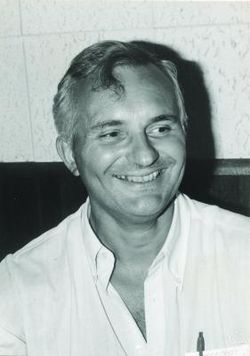
\includegraphics[width=\linewidth]{figures/lions.jpg}
%    \captionof*{figure}{\tiny J.L. Lions}
%  \end{minipage}}%
%  \hfill
%  \begin{minipage}[b]{0.46\textwidth}
%    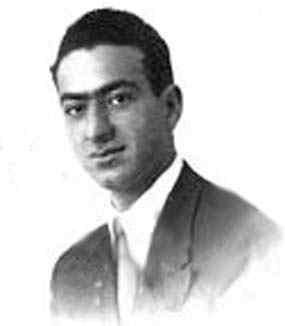
\includegraphics[width=\linewidth]{figures/stampacchia.jpg}
%    \captionof*{figure}{\tiny G. Stampacchia}
%  \end{minipage}
%\end{figure}\vspace{-6ex}
%\begin{figure}
%	\centering
%	\begin{tikzpicture}
%		\node at (-4.2,1.2) {\scriptsize 
%	    	$u$};
%		\node at (-3.35,0) {\includegraphics[height=1.25in]{figures/obstacle_new.png}};
%		\node at (-2.2,-1.35) {\scriptsize 
%	    	$\varphi$};
%    \end{tikzpicture}
%
%\end{figure}
%\end{minipage}
%\end{frame}

%\begin{frame}\frametitle{The Lions-Stampacchia Theorem}
%\begin{minipage}{0.6\linewidth}
%\begin{beamercolorbox}[rounded=true, shadow=true, wd=\textwidth]{block body}
%Comments:
%
%\begin{itemize}
%\item \visible<1->{For \textbf{symmetric $a$}, use the direct method.}
%\item \visible<2->{For \textbf{nonsymmetric $a$}: The proof embeds the nonsymmetric problem in a parametric fixed point iteration of the type $u = S_{\rho}(v)$ with parameter $\rho > 0$.}
%\item \visible<3->{The evaluation of $S_{\rho}(v)$ involves the solution of a related symmetric problem, which has a unique solution.}
%\item \visible<4->{After deriving several key estimates, it becomes clear what $\rho$ needs to be to ensure $S_{\rho}(v)$ is a contraction.}
%\end{itemize}
%
% \end{beamercolorbox}
%\end{minipage}\hspace{4ex}
%\begin{minipage}{0.3\linewidth}
% \centering
% \begin{figure}
%  \centering\vspace{1ex}
%  \visible<1->{\begin{minipage}[b]{0.45\textwidth}
%    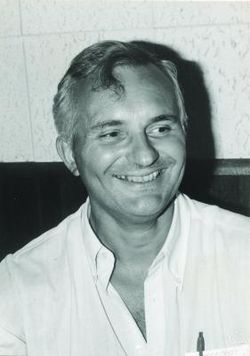
\includegraphics[width=\linewidth]{figures/lions.jpg}
%    \captionof*{figure}{\tiny J.L. Lions}
%  \end{minipage}}%
%  \hfill
%  \begin{minipage}[b]{0.46\textwidth}
%    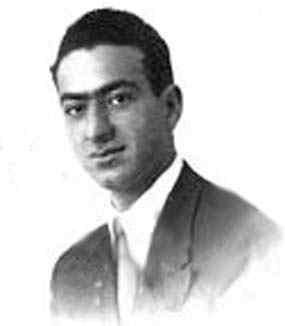
\includegraphics[width=\linewidth]{figures/stampacchia.jpg}
%    \captionof*{figure}{\tiny G. Stampacchia}
%  \end{minipage}
%\end{figure}\vspace{-6ex}
%\begin{figure}
%	\centering
%	\begin{tikzpicture}
%		\node at (-4.2,1.2) {\scriptsize 
%	    	$u$};
%		\node at (-3.35,0) {\includegraphics[height=1.25in]{figures/obstacle_new.png}};
%		\node at (-2.2,-1.35) {\scriptsize 
%	    	$\varphi$};
%    \end{tikzpicture}
%
%\end{figure}
%\end{minipage}
%\end{frame}

\subsection{Lagrange Multipliers}\label{sec:complementarity}
\begin{frame}\frametitle{Lagrange Multipliers}
%\begin{beamercolorbox}[rounded=true, shadow=true, wd=\textwidth]{block title}\centering
% \visible<1->{What distinguishes these problems from ordinary PDEs?}
% \end{beamercolorbox}
 
 \begin{center}
 \Large What distinguishes these problems from ordinary PDEs?
 \end{center}
 
%  \visible<2->{
% \begin{beamercolorbox}[rounded=true, shadow=true, wd=\textwidth]{block body}
%Consider again the VI for the Obstacle Problem: Find $u \in K$ such that
% \[
% (\nabla u, \nabla [v-u])_{L^2} \ge  (f,v-u)_{L^2} \quad \forall v \in K.
% \]
% 
% \visible<3->{
%Note $a(u,v) :=  (\nabla u, \nabla v)_{L^2}$ is a symmetric bounded continuous bilinear form.\medskip 
%
%We let  $A : V \to V^*$ be the associated bounded linear operator\footnote{\tiny Riesz Repr.\ Thm.: There exists (symmetric) bounded linear operator $A : V \to V^*$  $a(u,v) = \langle Au,v\rangle\quad \forall u,v \in V$.}
%}\vfill
%%\visible<4->{
%%Riesz Repr.\ Thm.: There exists (symmetric) bounded linear operator $A : V \to V^*$:
%% \[
%% a(u,v) = \langle Au,v\rangle\quad \forall u,v \in V.
%% \]
%% We then view the VI more abstractly: Find $u \in K$ such that
%% \[
%% \langle Au - f, v - u \rangle_{V^*,V} \ge 0 \quad \forall v \in K
%% \]\vspace{-3ex}
%% }
% \end{beamercolorbox}}
\end{frame}

\begin{frame}\frametitle{Lagrange Multipliers} \hypertarget{lagrange_mult}{}
  \visible<1->{
 \begin{beamercolorbox}[rounded=true, shadow=true, wd=\textwidth]{block body}
Introduce a \alert{slack variable} $\lambda := Au - f$ and consider the problem: Find $(u,\lambda) \in K \times V^*$:
\[\aligned
Au - \lambda &= f \quad\text{ in } V^*\\
\langle \lambda,v-u \rangle_{V^*,V} &\ge 0 \quad \forall v \in K.
\endaligned
\]
 \visible<2->{
What more can we say about $\lambda$?\medskip

}\visible<3->{
\begin{enumerate}
\item \visible<3->{$u \in K$ and $w \in H^1_0(\Omega)$ with $w \ge 0$ $\Rightarrow$ $u + w \ge \varphi$ and $(u + w)|_{\Gamma} = g$.}
\item \visible<4->{Setting $v = u + w$ implies $\langle \lambda, w \rangle \ge 0$ for all $w \in H^1_0(\Omega)$ : $w \ge 0$. \alert{``$\lambda \ge 0$''}\footnote{\tiny The Riesz-Schwarz theorem states $\lambda$ is in fact a nonnegative Radon measure on $\Omega$.}.}
%\item \visible<5->{The Riesz-Schwarz theorem states $\lambda$ is in fact a nonnegative Radon measure on $\Omega$.}
\item \visible<5->{
$
\mathrm{supp} \lambda \subset \mathcal{A} := \left\{x \in \Omega : u(x) = \varphi(x)\right\}.
$\footnote{\tiny Kinderlehrer-Stampacchia Thm. 6.9.}
\item  Hence, $\lambda(\left\{x \in \Omega : u(x) > \varphi(x)\right\}) = 0$
\hyperlink{target_lagrange}{\beamerbutton{explanation}}
%Proof uses smooth bump functions at points in $\mathcal{A}$ to get clever test functions.
}
\end{enumerate}
 }
 \end{beamercolorbox}}
\end{frame}

\begin{frame}\frametitle{Lagrange Multipliers: Final Words}
\begin{beamercolorbox}[rounded=true, shadow=true, wd=\textwidth]{block body}
 \visible<1->{If $u \in H^2(\Omega)$, then $Au - f \in L^2(\Omega)$ so $\lambda$ will have a \alert{pointwise} description:
 \[
 \lambda = \max\{0, \lambda - c (u - \varphi) \} \quad \text{ for any constant } c > 0
 \]}\vspace{-3ex}
 
 \visible<2->{In this setting, the set of $x \in \Omega$ where $\lambda = 0$ and $u = \varphi$ holds is called the \alert{biactive set}.\medskip
 
 }\visible<3->{A \alert{non-negligible biactive set} typically leads to worst-case convergence rates.\medskip
 
 
 } \visible<4->{In $H^1(\Omega)$, we \alert{cannot ignore $(n-1)$-dimensional subsets} of $\Omega$ on which $u(x) = \varphi(x)$.}
 \end{beamercolorbox}
 
% \visible<5->{
% \begin{beamercolorbox}[rounded=true, shadow=true, wd=\textwidth]{block title}
% For the general setting $\{\min J(u) \text{ over } V : G(u) \in C\}$ we get optimality conditions like
% \[
% 0 = dJ(u) +  d\langle \lambda, G(\cdot) \rangle(u)
% \]
% with $\lambda \in N_{C}(G(u)):= \left\{\mu : \langle \mu, y - G(u) \rangle \le 0 \quad \forall y \in C\right\}$.
%  \end{beamercolorbox}
%  }
\end{frame}

\subsection{Computational Aspects}\label{sec:algorithms}
%\begin{frame}{Algorithms}
%    \begin{enumerate}
%        \item Penalty
%        \item Barrier
%        \item Augmented Lagrangian
%    \end{enumerate}
%\end{frame}

\begin{frame}\frametitle{Towards Solution Algorithms}
\begin{beamercolorbox}[rounded=true, shadow=true, wd=\textwidth]{block body}\centering
 \visible<1->{How does one actually \alert{solve} a variational inequality?}
 \end{beamercolorbox}\hfill
 \visible<2->{
% \begin{minipage}{0.6\textwidth}
 \begin{beamercolorbox}[rounded=true, shadow=true, wd=\textwidth]{block body}\centering
 First Idea: Use a Ritz-Galerkin approach by replacing $V$ by $V_{h}$. Then use a black box optimization solver, e.g., active set method. 
 \end{beamercolorbox}}
 \hfill
  \visible<3->{
% \begin{minipage}{0.6\textwidth}
 \begin{beamercolorbox}[rounded=true, shadow=true, wd=\textwidth]{block title}\centering
What might be the issues with such an approach?
 \end{beamercolorbox}}
% \end{minipage}}%\quad\quad
% %
% \begin{minipage}{0.33\textwidth}\vspace{3ex}
%% \begin{beamercolorbox}[rounded=true, shadow=true, wd=\textwidth]{block body}
% \centering\visible<3->{
% \resizebox{\textwidth}{\textwidth}{%
%\begin{tikzpicture}
%\begin{axis}[
%%    width=\linewidth,
%%    height=4cm,
%    scale only axis,
%    axis lines=middle,
%    xlabel={$x$},
%    ylabel={$\phi_i(x)$},
%    xtick={0, 0.5, 1},
%    xticklabels={$x_0$, $x_1$, $x_2$},
%    ytick={-0.5, 0, 0.5, 1},
%    ymin=-0.6, ymax=1.2,
%    xmin=0, xmax=1,
%    legend style={font=\tiny, at={(1.0,-0.1)}, anchor=north east},
%    grid=major,
%    domain=0:1,
%    samples=200
%]
%
%\addplot[red, thick, dashed] {2*(x - 0.5)*(x - 1)};
%\addlegendentry{$\phi_0(x)$}
%
%\addplot[blue, thick] {-4*x*(x - 1)};
%\addlegendentry{$\phi_1(x)$}
%
%\addplot[green!60!black, thick, dashdotted] {2*x*(x - 0.5)};
%\addlegendentry{$\phi_2(x)$}
%
%\end{axis}
%\end{tikzpicture}
%}}
%% \end{beamercolorbox} 
% \end{minipage}
 
 \end{frame}
 
 
%  \begin{frame}\frametitle{Potential Issues}
%   \visible<1->{
% \begin{beamercolorbox}[rounded=true, shadow=true, wd=\textwidth]{block title}\centering
%Black box optimization solvers typically use the Euclidean inner product for computing gradients. Why is that a problem?
% \end{beamercolorbox}}
% 
% \visible<2->{
% \begin{beamercolorbox}[rounded=true, shadow=true, wd=\textwidth]{block body}
%Consider 
%$
%J(u) := \frac{1}{2} \| \nabla u \|^2_{L^2(\Omega)} - (f,u)_{L^2(\Omega)}
%$,
%%  \text{ with } u \in H^1_0(\Omega), f \in L^2(\Omega)$, 
%with directional \alert{derivative} \visible<3->{
%\[
%dJ(u)\delta = (\nabla u, \nabla \delta)_{L^2(\Omega)} - (f,\delta)_{L^2(\Omega)} \quad \delta \in H^1_0(\Omega). 
%\]}\visible<4->{The derivative is a \alert{dual quantity}, i.e., an element of $H^{-1}(\Omega)$. }\medskip
%
%\visible<5->{But \alert{gradient}\footnote{\tiny By the Riesz Representation Theorem} $\nabla J(u)$ is a \alert{primal} quantity:
%\[
%\nabla J(u) = u - (-\Delta)^{-1} f.
%\]
%}\vspace{-3ex}
%%the unique solution $y$ to
%%\[
%%(\nabla y, \nabla \varphi)_{L^2(\Omega)} = (\nabla u, \nabla \varphi)_{L^2(\Omega)} - (f,\varphi)_{L^2(\Omega)} \quad \forall \varphi \in H^1_0(\Omega).
%%\]}\visible<5->{
%%E.g. $f \equiv 0$ implies $\nabla J(u) = u$. In general, $\nabla J(u) = u - (-\Delta)^{-1} f.$}
% \end{beamercolorbox}}
% \end{frame}
% 
   \begin{frame}\frametitle{Potential Issues}
   \visible<1->{
 \begin{beamercolorbox}[rounded=true, shadow=true, wd=\textwidth]{block title}\centering
Black box optimization solvers typically use the Euclidean inner product for computing gradients. Why is that a problem?
 \end{beamercolorbox}}
 
 \visible<2->{
 \begin{beamercolorbox}[rounded=true, shadow=true, wd=\textwidth]{block body}
Consider 
$
J(u) := \frac{1}{2} \| \nabla u \|^2_{L^2(\Omega)} - (f,u)_{L^2(\Omega)}
$.\medskip

\visible<3->{
The \alert{true} $H^1$-gradient: $\nabla J(u) = u - (-\Delta)^{-1} f.$
}\medskip

\visible<4->{
After discretization, $J$ becomes $J_h(\mathbf{u}) = \frac{1}{2} \mathbf{u}^T A_h \mathbf{u} - \mathbf{f}^T M_h \mathbf{u} \text{ with } \mathbf{u}, \mathbf{f} \in \mathbb R^n$
}\medskip

\visible<5->{The \alert{ill-conditioned}\footnote{\tiny The condition number of $A_h$ grows like $O(h^{-2})$} \alert{gradient} in $\mathbb R^n$ is 
$\nabla J_h(\mathbf{u}) := A_h \mathbf{u} - M_h \mathbf{f}$
}\medskip

\visible<6->{
The \alert{properly conditioned} gradient in $V_h$ is $\nabla J_h(\mathbf{u}) = A^{-1}_h(A_h \mathbf{u} - M_h \mathbf{f}) = \mathbf{u} - A^{-1}_h M_h \mathbf{f}$.\medskip

Most solvers do not do this automatically. 
}
 \end{beamercolorbox}}
 \end{frame}
 
 
%   \begin{frame}\frametitle{Potential Issues}
%    \visible<1->{
% \begin{beamercolorbox}[rounded=true, shadow=true, wd=\textwidth]{block body}
%If we ``\alert{first discretize, then optimize}'', then we feed the solver a discretized objective
%\[
%J_h(\mathbf{u}) := \frac{1}{2} \mathbf{u}^T A_h \mathbf{u} - \mathbf{f}^T M_h \mathbf{u}\quad \text{ with }\quad \mathbf{u}, \mathbf{f} \in \mathbb R^n,
%\]
%with mesh parameter $h > 0$, whose gradient in $\mathbb R^n$ is given by
%\[
%\nabla^{\mathbb R^n} J_h(\mathbf{u}) := A_h \mathbf{u} - M_h \mathbf{f}.
%\]
%\visible<2->{Let $\mathbf{f} \equiv 0$. Now the gradient is $A_h \mathbf{u}$, where  \alert{the condition number of $A_h$ is $O(h^{-2})$!}\medskip 
%}
%
%\visible<3->{The gradient associated with the finite dimensional subspace $V_h$, however, should be
% \[
%\nabla^{V_h} J_h(\mathbf{u}) := A^{-1}_h(A_h \mathbf{u} - M_h \mathbf{f}) = \mathbf{u} - A^{-1}_h M_h \mathbf{f},
%\]
%which fixes the conditioning. Most solvers do not do this automatically. 
%}
%
% \end{beamercolorbox}}
% \end{frame}
 
% \begin{frame}\frametitle{Potential Issues}
%   \visible<1->{
% \begin{beamercolorbox}[rounded=true, shadow=true, wd=\textwidth]{block title}\centering
%Black box optimization solvers typically use the Euclidean inner product for computing gradients. Why is that a problem?
% \end{beamercolorbox}}
% 
% \visible<2->{
% \begin{beamercolorbox}[rounded=true, shadow=true, wd=\textwidth]{block body}
%Consider 
%$
%J(u) := \frac{1}{2} \| \nabla u \|^2_{L^2(\Omega)} - (f,u)_{L^2(\Omega)}  \text{ with } u \in H^1_0(\Omega), f \in L^2(\Omega).
%$
%\visible<3->{The \alert{derivative} in $H^1_0(\Omega)$ in $u$ in direction $\delta \in H^1_0(\Omega)$ is:
%\[
%dJ(u)\delta = (\nabla u, \nabla \delta)_{L^2(\Omega)} - (f,\delta)_{L^2(\Omega)}.
%\]
%The derivative is a \alert{dual quantity}, i.e., an element of $H^{-1}(\Omega)$. }\visible<4->{But the Riesz Rep.\ Thm.\, says the \alert{gradient} $\nabla J(u)$ is the unique solution $y$ to
%\[
%(\nabla y, \nabla \varphi)_{L^2(\Omega)} = (\nabla u, \nabla \varphi)_{L^2(\Omega)} - (f,\varphi)_{L^2(\Omega)} \quad \forall \varphi \in H^1_0(\Omega).
%\]}\visible<5->{
%E.g. $f \equiv 0$ implies $\nabla J(u) = u$. In general, $\nabla J(u) = u - (-\Delta)^{-1} f.$}
% \end{beamercolorbox}}
% \end{frame}
 
%  \begin{frame}\frametitle{Potential Issues}
%    \visible<1->{
% \begin{beamercolorbox}[rounded=true, shadow=true, wd=\textwidth]{block body}
%If we ``\alert{first discretize, then optimize}'', then we feed the solver a discretized objective
%\[
%J_h(\mathbf{u}) := \frac{1}{2} \mathbf{u}^T A_h \mathbf{u} - \mathbf{f}^T M_h \mathbf{u}\quad \text{ with }\quad \mathbf{u}, \mathbf{f} \in \mathbb R^n,
%\]
%with mesh parameter $h > 0$, whose gradient in $\mathbb R^n$ is given by
%\[
%\nabla^{\mathbb R^n} J_h(\mathbf{u}) := A_h \mathbf{u} - M_h \mathbf{f}.
%\]
%\visible<2->{Let $\mathbf{f} \equiv 0$. Now the gradient is $A_h \mathbf{u}$, where  \alert{the condition number of $A_h$ is $O(h^{-2})$!}\medskip 
%}
%
%\visible<3->{The gradient associated with the finite dimensional subspace $V_h$, however, should be
% \[
%\nabla^{V_h} J_h(\mathbf{u}) := A^{-1}_h(A_h \mathbf{u} - M_h \mathbf{f}) = \mathbf{u} - A^{-1}_h M_h \mathbf{f},
%\]
%which fixes the conditioning. Most solvers do not do this automatically. 
%}
%
% \end{beamercolorbox}}
% \end{frame}
 
\begin{frame}\frametitle{Potential Issues}

\begin{minipage}{0.55\linewidth}
 \begin{beamercolorbox}[rounded=true, shadow=true, wd=\textwidth]{block body}
% \visible<1->{Recall the 
% \textbf{mixed complementarity problem}:}\medskip
% 
 \visible<1->{Find $(u,\lambda) \in H^1_0(\Omega) \times H^{-1}(\Omega)$ s.t.
\[
\underbrace{-\Delta u - \lambda = f,}_{\text{PDE}} \quad \underbrace{u \ge 0 \quad {\color{red}``\lambda \ge 0"} \quad \langle \lambda, u \rangle = 0}_{\text{Complementarity Condition}}.
\]}
 \end{beamercolorbox}
\end{minipage}\quad
\begin{minipage}{0.4\linewidth}
\centering\visible<1->{
	\begin{tikzpicture}
		\node at (-1.35,1.25) {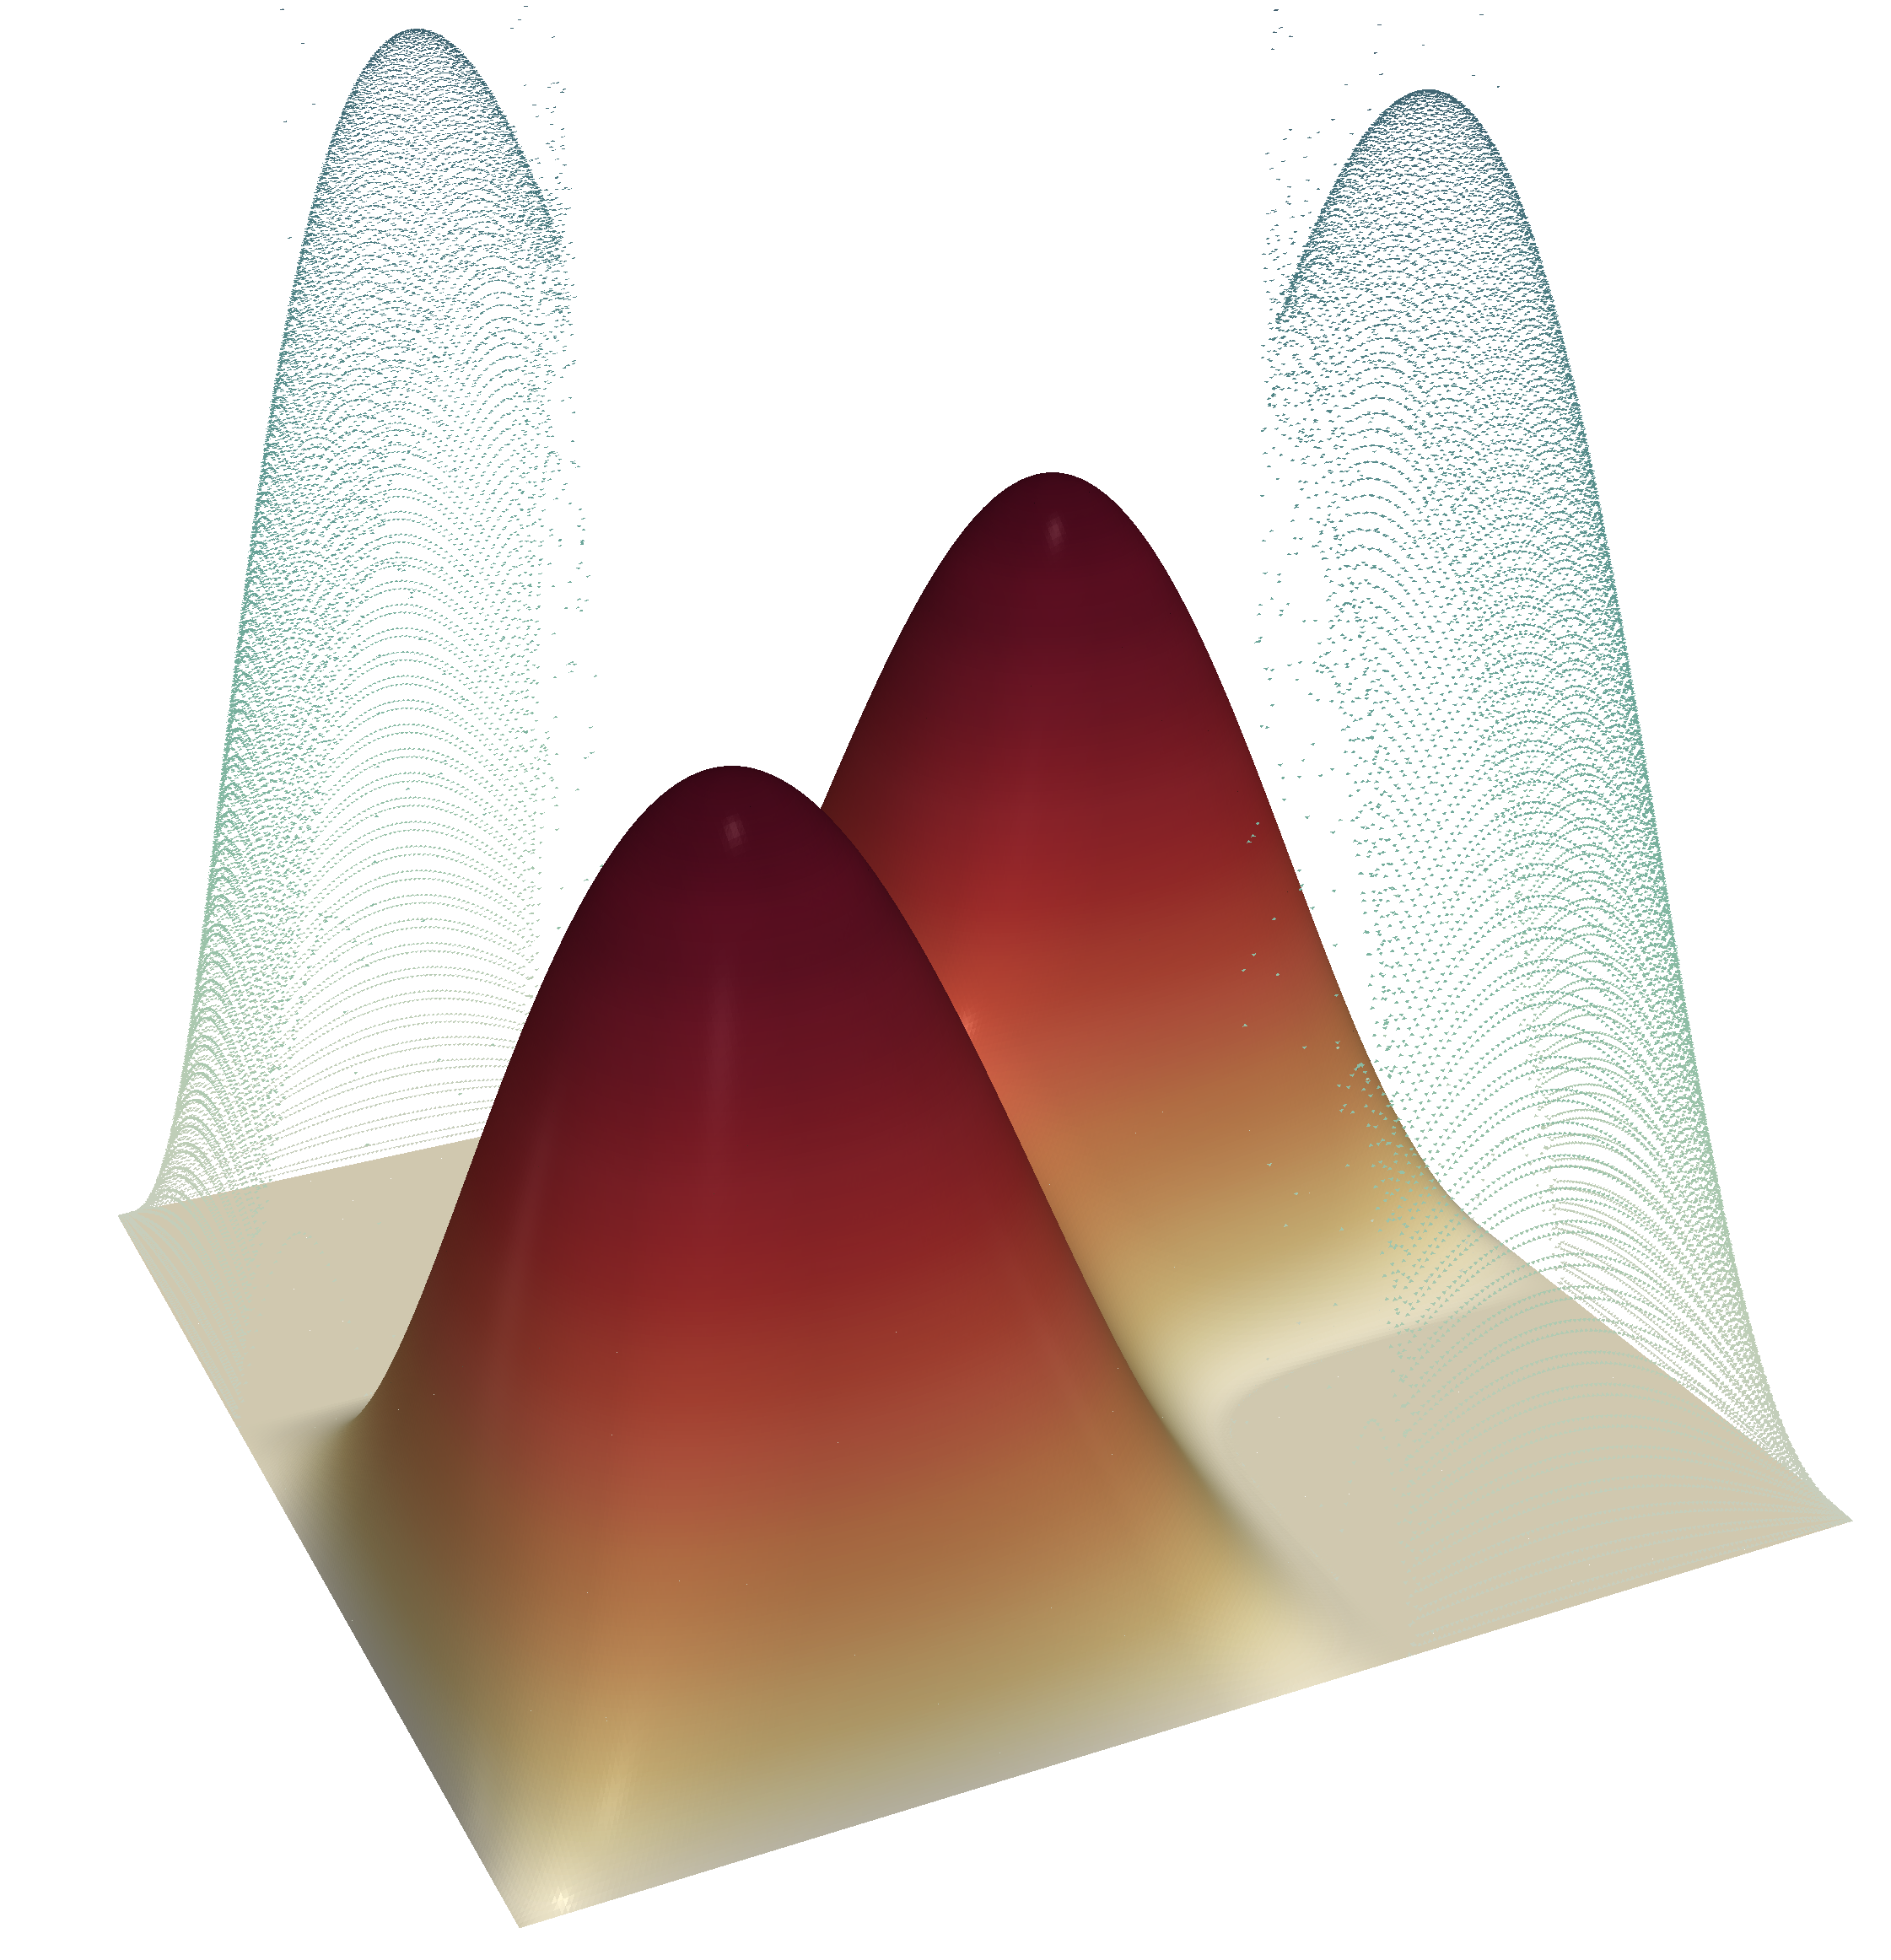
\includegraphics[clip=true, trim= 4cm 0 0 0, height=4cm]{figures/ObstacleExperiment2.png}};
		% \node at (-3.35,1) {
\includegraphics[clip=true, trim= 4cm 0 0 0, width=0.44\textwidth]{Figures/ObstacleExperiment2.png}};
%		\node at (3,0.4) {
%		   \includegraphics[clip=true, trim= 0 0 0.35cm 0, height=2.1in]{Figures/tikz/FEniCS_plots/example1/example1_ConvergenceRate.pdf}
%		};
	    % \node at (-4,2.8) {
\includegraphics[height=2cm]{Figures/tikz/FEniCS_plots/example1/colorbar/colorbar1.pdf}};
	    \node at (-3.7,0.5) {
\includegraphics[height=2cm]{figures/colorbar1.pdf}};
	    \node at (0.75,2.2) {
\includegraphics[height=2cm]{figures/colorbar2.pdf}};
    \end{tikzpicture}
}
\end{minipage}\medskip

\visible<2->{
%\begin{minipage}{0.48\linewidth}
\begin{beamercolorbox}[rounded=true, shadow=true, wd=\textwidth]{block body}
The \alert{low regularity of the Lagrange multiplier} will result in a numerical method that requires more iterations to reach the same stopping tolerance on increasingly finer meshes. This is known as \alert{mesh dependence}.
%$\lambda$ has low regularity. 
% 
%This results in \textit{mesh dependence}
%%\footnote{\tiny The number of iterations needed to reach the same stopping tolerance increases with mesh refinements.} 
% for methods tacitly requiring $\lambda \in L^2(\Omega)$.
\end{beamercolorbox}
%\end{minipage}
}
%\visible<5->{
%\begin{minipage}{0.48\linewidth}
% \begin{beamercolorbox}[rounded=true, shadow=true, wd=\textwidth]{block title}
%$\text{Leb}(\left\{x \in \Omega : u(x) = 0,\; \lambda(x) = 0 \right\}) > 0$ causes numerical instabilities.
%
%\centering
%``Loss of strict complementarity''
%\end{beamercolorbox}
%\end{minipage}
%}


\end{frame}
 
 \begin{frame}\frametitle{Potential Issues}
   \begin{beamercolorbox}[rounded=true, shadow=true, wd=\textwidth]{block title}\centering
  Can we faithfully discretize the inequality constraints?
   \end{beamercolorbox}
 \visible<2->{
 \begin{minipage}{0.6\textwidth}
 \begin{beamercolorbox}[rounded=true, shadow=true, wd=\textwidth]{block body}
\visible<2->{
Brezis \& Stampacchia (1968): The regularity theory for the obstacle problem is very similar to Poisson.\medskip 

$u \in H^2(\Omega)$ if $\Gamma$, $f$, and $\varphi$ are sufficiently regular.
}
\end{beamercolorbox}
\visible<3->{   
\begin{beamercolorbox}[rounded=true, shadow=true, wd=\textwidth]{block body}  
\visible<3->{This opens the door for higher order bases, $hp$-refinement, etc. \alert{However,...}
}

\visible<4->{ \medskip
If the basis elements are not non-negative, then the discrete solution $u_{h}$ will not be globally feasible!
 }
 \end{beamercolorbox}}
 \end{minipage}}\quad\quad
 %
 \begin{minipage}{0.3\textwidth}\vspace{3ex}
% \begin{beamercolorbox}[rounded=true, shadow=true, wd=\textwidth]{block body}
 \centering\visible<3->{
 \resizebox{\textwidth}{\textwidth}{%
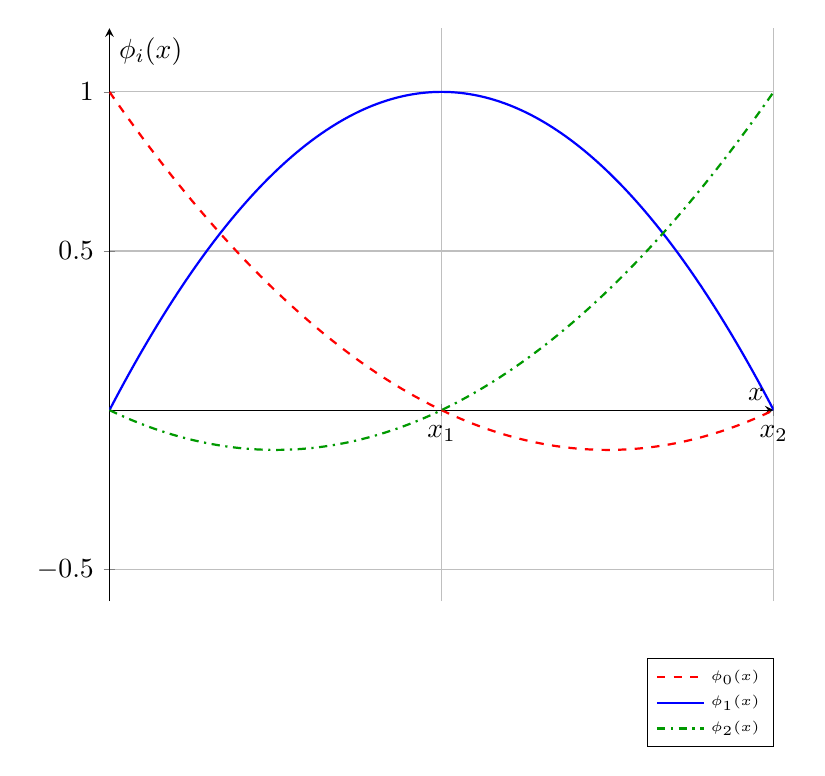
\begin{tikzpicture}
\begin{axis}[
%    width=\linewidth,
%    height=4cm,
    scale only axis,
    axis lines=middle,
    xlabel={$x$},
    ylabel={$\phi_i(x)$},
    xtick={0, 0.5, 1},
    xticklabels={$x_0$, $x_1$, $x_2$},
    ytick={-0.5, 0, 0.5, 1},
    ymin=-0.6, ymax=1.2,
    xmin=0, xmax=1,
    legend style={font=\tiny, at={(1.0,-0.1)}, anchor=north east},
    grid=major,
    domain=0:1,
    samples=200
]

\addplot[red, thick, dashed] {2*(x - 0.5)*(x - 1)};
\addlegendentry{$\phi_0(x)$}

\addplot[blue, thick] {-4*x*(x - 1)};
\addlegendentry{$\phi_1(x)$}

\addplot[green!60!black, thick, dashdotted] {2*x*(x - 0.5)};
\addlegendentry{$\phi_2(x)$}

\end{axis}
\end{tikzpicture}
}}
% \end{beamercolorbox} 
 \end{minipage}
% \visible<5->{
%  \begin{beamercolorbox}[rounded=true, shadow=true, wd=\textwidth]{block title}\centering
%Non-negativity is not enough: There are linear combinations of Bernstein polynomials that are globally nonnegative but which have some negative coefficients!
%   \end{beamercolorbox}
% }
\end{frame}


 \begin{frame}\frametitle{Summary}
      \begin{beamercolorbox}[rounded=true, shadow=true, wd=\textwidth]{block body}
An \alert{\bf{ideal solver}} is...\medskip

%\begin{enumerate}
%\item 
...designed in accordance with the infinite-dimensional nature of the problem.\medskip

%\item 
...provably (or observably) mesh independent for standard stopping criteria.\medskip

%\item 
...able to provide a globally constraint-preserving representation of $u$ (or $G(u)$ in general).
%\end{enumerate}
 \end{beamercolorbox}
 \hfill
\visible<2->{
 \begin{beamercolorbox}[rounded=true, shadow=true, wd=\textwidth]{block body}
From a \alert{\bf{practical standpoint}}, an \alert{\bf{ideal solver}} should be...\medskip 
%\begin{enumerate}
%\item 

...fast to converge.\medskip

%\item 
...have a low computational cost per iteration.\medskip

%\item 
...easy to implement
%\end{enumerate}
   \end{beamercolorbox}}
 \end{frame}


\section{Approximation Methods}
\subsection{Outer and Inner Approximation Methods}
% \begin{frame}\frametitle{Frame Title}
%    \begin{enumerate}
%    	\item Quadratic Penalty
%		\begin{enumerate}
%			\item Definition
%			\item Connection to Moreau-Yosida regularization
%			\item Asymptotic convergence
%			\item Advantages/Disadvantages
%			\item Path-following
%		\end{enumerate}
%	\item Barrier Penalty
%		\begin{enumerate}
%			\item Definition
%			\item Outer vs. Inner approximation
%			\item Primal-dual formulation
%			\item PD does not force $u$ to be nonnegative, this has to be done with careful line search
%		\end{enumerate}
%	\item Augmented Lagrangian (Ito, Kunisch 1990)
%		\begin{enumerate}
%			\item Definition
%			\item A dual-adaptive quadratic penalty scheme, roots in proximal point (Rockafellar)
%			\item For computation, we need $\lambda$ to have a pointwise interpretation, but this may not be guaranteed
%			\item This forces $r \to +\infty$ (as opposed to finite dimensions)
%		\end{enumerate}
%    \end{enumerate}
% \end{frame}
 
 \begin{frame}\frametitle{A Mathematical Fruitfly} 
  \begin{beamercolorbox}[rounded=true, shadow=true, wd=\textwidth]{block title}\centering
  In order to make a nuanced comparison between several methods, we introduce each method using the obstacle problem.
  The methods themselves are widely applicable.
  \end{beamercolorbox}\hfill
  
\visible<2->{
\begin{minipage}{0.7\linewidth}
\begin{beamercolorbox}[rounded=true, shadow=true, wd=\textwidth]{block body}
 We seek a minimizer $u$ of the objective functional:
 \begin{equation*}
 	J(v)
 	=
 	\frac{1}{2}
 	\int_\Omega |\nabla v|^2 \dd x
 	-
 	\int_\Omega f v\dd x
 	\,,
 \end{equation*}
 over
 \[
 K = \{ v \in H^1_0(\Omega) \mid  v \ge \varphi \text{~a.e. }  \}.
 \] 
 Here, $f \in L^2(\Omega)$ and  $\varphi \in H^1(\Omega)$, $\varphi|_{\Gamma} \le 0$.
\end{beamercolorbox}
\end{minipage}%
\begin{minipage}{0.3\linewidth}
 \centering
\begin{figure}
	\centering
	\begin{tikzpicture}
		\node at (-4.2,1.2) {\scriptsize 
	    	$u$};
		\node at (-3.35,0) {\includegraphics[height=1.25in]{../Part I/figures/obstacle_new.png}};
		\node at (-2.2,-1.35) {\scriptsize 
	    	$\varphi$};
    \end{tikzpicture}
\end{figure}
\end{minipage}}
 \end{frame}
 
% \begin{frame}\frametitle{Penalty Methods}
%   \begin{beamercolorbox}[rounded=true, shadow=true, wd=\textwidth]{block body}
%This approach involves relaxing the constraints with a smooth penalty function $\beta : V \to \mathbb R$, where $\beta$ is usually convex, $C^{1,1}$ and ideally satisfies
%\[
%\beta(u) = 0 \text{ if } u \in K\quad \text{ and }\quad \beta(u) > 0 \text{ otherwise. }
%\]
%  \end{beamercolorbox}
%%\begin{minipage}{\textwidth}
%% \centering 
% \begin{figure}
%% \resizebox{0.3\textwidth}{0.25\textwidth}{%
%  \begin{tikzpicture}[scale=0.5]
%    \begin{axis}[
%        axis lines=middle, % Draw axes through the origin
%        xlabel=$x$,
%        ylabel=$\beta_\gamma(x)$,
%        xmin=-2, xmax=2, % Adjust x-range as needed
%        ymin=-0.5, ymax=10, % Adjust y-range as needed
%        grid=both, % Add a grid
%        grid style={line width=.1pt, draw=gray!10}, % Style the grid lines
%        major grid style={line width=.2pt,draw=gray!50}, % Style major grid lines
%        xtick distance=1, % Tick marks every 1 unit on x-axis
%        ytick distance=1, % Tick marks every 1 unit on y-axis
%        % Add a legend
%        legend pos=outer north east, % Position the legend
%        legend cell align=left,
%        no markers, % Don't put markers on the plots
%    ]
%
%    % Define the function with a placeholder for c
%    % We use 'max(0,x)^2' for the (x)^2 part, and then multiply by c
%    % PGFPlots works with degrees, so we need to be careful with functions that are not trigonometric.
%    % max(0, x) is directly supported.
%
%    % Plot for c = 0.5
%    \addplot[domain=-2:4, ForestGreen, ultra thick] {1 * max(0,-x)^2};
%    \addlegendentry{$\gamma=1$};
%
%    % Plot for c = 1
%    \addplot[domain=-2:4, MidnightBlue, ultra thick] {10.0 * max(0,-x)^2};
%    \addlegendentry{$\gamma=10$};
%
%    % Plot for c = 2
%    \addplot[domain=-2:4, BurntOrange, ultra thick] {50.0 * max(0,-x)^2};
%    \addlegendentry{$\gamma=100$};
%
%    \end{axis}
%\end{tikzpicture}
%%}
%\caption{Plot of typical quadratic penalty function used for inequality constraints $\beta_\gamma(x) = \gamma\max\{0,-x\}^2$.}
%  \label{fig:tikz-example}
%\end{figure}
%%\end{minipage}
% \end{frame}
 
  \begin{frame}\frametitle{Quadratic Penalty Methods}
  \begin{minipage}{0.67\linewidth}
\begin{beamercolorbox}[rounded=true, shadow=true, wd=\textwidth]{block body}
 Given $\gamma > 0$, we seek a minimizer $u_{\gamma} \in H^1_0(\Omega)$ of the objective functional:
 \begin{equation*}
 	J_{\gamma}(v)
 	=
 	\frac{1}{2}
 	\int_\Omega |\nabla v|^2 \dd x
 	-
 	\int_\Omega f v\dd x
	+
	\frac{\gamma}{2}\int_{\Omega} \max\{0,\varphi - v\}^2 \dd x
%	\underbrace{\frac{\gamma}{2}\int_{\Omega} \max\{0,\varphi - v\}^2 \dd x}_{=:\gamma \beta(v)}
 	\,.
 \end{equation*}
 Here, $f \in L^2(\Omega)$ and  $\varphi \in H^1(\Omega)$, $\varphi|_{\Gamma} \le 0$.
\end{beamercolorbox}
\end{minipage}\hfill
\begin{minipage}{0.3\linewidth}
 \begin{figure}
% \resizebox{0.3\textwidth}{0.25\textwidth}{%
  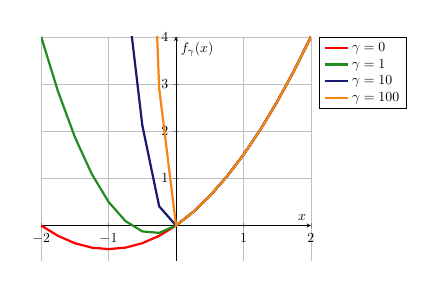
\begin{tikzpicture}[scale=0.5]
    \begin{axis}[
        axis lines=middle, % Draw axes through the origin
        xlabel=$x$,
        ylabel=$f_\gamma(x)$,
        xmin=-2, xmax=2, % Adjust x-range as needed
        ymin=-0.75, ymax=4, % Adjust y-range as needed
        grid=both, % Add a grid
        grid style={line width=.1pt, draw=gray!10}, % Style the grid lines
        major grid style={line width=.2pt,draw=gray!50}, % Style major grid lines
        xtick distance=1, % Tick marks every 1 unit on x-axis
        ytick distance=1, % Tick marks every 1 unit on y-axis
        % Add a legend
        legend pos=outer north east, % Position the legend
        legend cell align=left,
        no markers, % Don't put markers on the plots
    ]

    % Define the function with a placeholder for c
    % We use 'max(0,x)^2' for the (x)^2 part, and then multiply by c
    % PGFPlots works with degrees, so we need to be careful with functions that are not trigonometric.
    % max(0, x) is directly supported.


    \addplot[domain=-2:4, Red, ultra thick] {0.5*x^2 + 1*x + 0 * max(0,-x)^2};
    \addlegendentry{$\gamma=0$};
    % Plot for c = 0.5
    \addplot[domain=-2:4, ForestGreen, ultra thick] {0.5*x^2 + 1*x + 1 * max(0,-x)^2};
    \addlegendentry{$\gamma=1$};

    % Plot for c = 1
    \addplot[domain=-2:4, MidnightBlue, ultra thick] {0.5*x^2 + 1*x + 10.0 * max(0,-x)^2};
    \addlegendentry{$\gamma=10$};

    % Plot for c = 2
    \addplot[domain=-2:4, BurntOrange, ultra thick] {0.5*x^2 + 1*x + 50.0 * max(0,-x)^2};
    \addlegendentry{$\gamma=100$};

    \end{axis}
\end{tikzpicture}
%}
\caption{\scriptsize Plot of $f_\gamma(x) = \frac{1}{2} x^2 + x + \gamma\max\{0,-x\}^2$}
  \label{fig:tikz-example}
\end{figure}
\end{minipage}

\hypertarget{penalty}{}
\hyperlink{target_workflow}{\beamerbutton{workflows for approximation methods}}

      \visible<2->{
 \begin{beamercolorbox}[rounded=true, shadow=true, wd=\textwidth]{block title}\centering
The conditioning issues and lack of feasibilty are a major downside of penalty methods.
 \end{beamercolorbox}}\hfill   
  \end{frame}
  
%\begin{frame}\frametitle{Augmented Lagrangian Method}
%      \visible<1->{
% \begin{beamercolorbox}[rounded=true, shadow=true, wd=\textwidth]{block title}\centering
%The conditioning issues and lack of guarantees for feasibilty are a major downside of penalty methods.
% \end{beamercolorbox}}\hfill   
% 
%       \visible<2->{
% \begin{beamercolorbox}[rounded=true, shadow=true, wd=\textwidth]{block body}\centering
%Finite-dimensional nonlinear optimization offers a (sort of) remedy to this problem in the form of the \alert{Augmented Lagrangian Method}.
% \end{beamercolorbox}}\hfill    
% 
%       \visible<3->{
% \begin{beamercolorbox}[rounded=true, shadow=true, wd=\textwidth]{block body}\centering
%In \alert{finite dimensions} we do not require the penalty parameter to pass to infinity for AL.
% \end{beamercolorbox}}
%\end{frame}

  \begin{frame}\frametitle{Augmented Lagrangian Method}
  \begin{minipage}{0.68\linewidth}
\begin{beamercolorbox}[rounded=true, shadow=true, wd=\textwidth]{block body}
 Given $\gamma > 0$, and a Lagrange multiplier $\lambda$, we define the \alert{Lagrangian} and \alert{Augmented Lagrangian}, resp.:
 \begin{equation*}\aligned \visible<1->{
  	L(v,\lambda)
 	&=
	\frac{1}{2}\| \nabla v \|^2 - (f,v) - \langle \lambda, v-\varphi\rangle}\\\visible<2->{
 	L(v,\lambda,\gamma)
 	&=
 	\frac{1}{2}\| \nabla v \|^2 - (f,v) -  \| \lambda\|^2 + 
%	&\hspace{8ex}+
	\frac{1}{2\gamma}\|(\lambda + \gamma (\varphi - u))_+\|^2}
 	\endaligned
 \end{equation*}
\end{beamercolorbox}
\end{minipage}\hfill
\begin{minipage}{0.3\linewidth}
 \begin{figure}
% \resizebox{0.3\textwidth}{0.25\textwidth}{%
  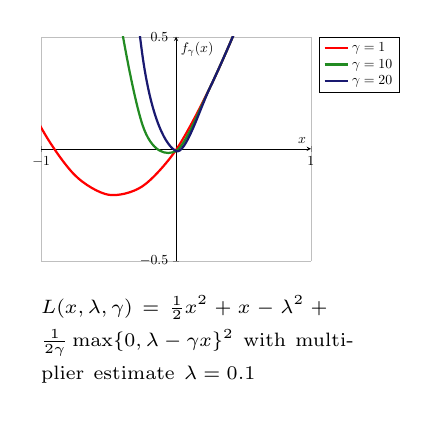
\begin{tikzpicture}[scale=0.5]
    \begin{axis}[
        axis lines=middle, % Draw axes through the origin
        xlabel=$x$,
        ylabel=$f_\gamma(x)$,
        xmin=-1, xmax=1, % Adjust x-range as needed
        ymin=-0.5, ymax=.5, % Adjust y-range as needed
        grid=both, % Add a grid
        grid style={line width=.1pt, draw=gray!10}, % Style the grid lines
        major grid style={line width=.2pt,draw=gray!50}, % Style major grid lines
        xtick distance=1, % Tick marks every 1 unit on x-axis
        ytick distance=.5, % Tick marks every 1 unit on y-axis
        % Add a legend
        legend pos=outer north east, % Position the legend
        legend cell align=left,
        no markers, % Don't put markers on the plots
    ]

    % Define the function with a placeholder for c
    % We use 'max(0,x)^2' for the (x)^2 part, and then multiply by c
    % PGFPlots works with degrees, so we need to be careful with functions that are not trigonometric.
    % max(0, x) is directly supported.


    \addplot[domain=-2:4, Red, ultra thick, smooth] {0.5*x^2 + 1*x  - 0.1^2 + 1 * max(0,0.1-x)^2 / 2};
    \addlegendentry{$\gamma=1$};
    % Plot for c = 0.5
    \addplot[domain=-2:4, ForestGreen, ultra thick,smooth] {0.5*x^2 + 1*x  - 0.1^2 + max(0,0.1-10*x)^2 / (2*10)};
    \addlegendentry{$\gamma=10$};

    % Plot for c = 1
    \addplot[domain=-2:4, MidnightBlue, ultra thick, smooth] {0.5*x^2 + 1*x - 0.1^2+  max(0,0.1-20*x)^2 / (2*20)};
    \addlegendentry{$\gamma=20$};

    % Plot for c = 2
%    \addplot[domain=-2:4, BurntOrange, ultra thick] {0.5*x^2 + 1*x  - x + 50.0 * max(0,-x)^2 * 0.5};
%    \addlegendentry{$\gamma=50$};
	
    \end{axis} \node[text width=4cm, align=left] at (4,-2) {\scriptsize $L(x,\lambda,\gamma) =\frac{1}{2} x^2 + x -\lambda^2 + \frac{1}{2\gamma}\max\{0,\lambda-\gamma x\}^2$ with multiplier estimate $\lambda = 0.1$};
\end{tikzpicture}
%}
%\caption{\scriptsize Plot of $L(x,\lambda,\gamma) =\frac{1}{2} x^2 + x -\lambda + \gamma\max\{0,-x\}^2$ with $\lambda = 0.5$}
  \label{fig:tikz-example}
\end{figure}
\end{minipage}
      \visible<3->{
 \begin{beamercolorbox}[rounded=true, shadow=true, wd=\textwidth]{block title}\centering
In light of the theory of Lagrange multipliers for the obstacle problem ($\lambda \in H^{-1}(\Omega) \cap M(\Omega)$), there is a clear discrepancy. Here, we need $\lambda \in L^2(\Omega)$.
 \end{beamercolorbox}}\hfill   
  \end{frame}
  


\begin{frame}\frametitle{Interior Point Methods}
        \visible<1->{
 \begin{beamercolorbox}[rounded=true, shadow=true, wd=\textwidth]{block title}\centering
The previously sketched methods approximate the feasible set $K$ from ``the outside''. Classical interior point methods offer an alternative viewpoint.
\end{beamercolorbox}}   \vspace{3ex}
\visible<2->{
  \begin{minipage}{0.67\linewidth}
\begin{beamercolorbox}[rounded=true, shadow=true, wd=\textwidth]{block body}
 Given $\mu > 0$, use a \alert{logarithmic barrier function} and consider
 \begin{equation*}
 	J_{\mu}(v)
 	=
 	\frac{1}{2}
 	\int_\Omega |\nabla v|^2 \dd x
 	-
 	\int_\Omega f v\dd x
	-
	\mu \int_{\Omega} \ln(u-\varphi) \dd x
 	\,.
 \end{equation*}
\end{beamercolorbox}
\end{minipage}\hfill
\begin{minipage}{0.3\linewidth}
 \begin{figure}
 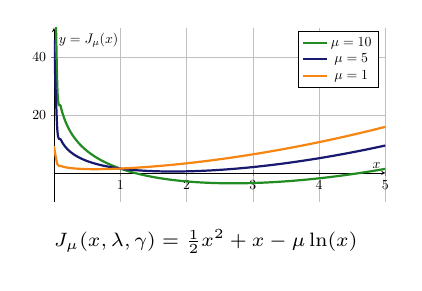
\begin{tikzpicture}[scale=0.5]
  \begin{axis}[
    domain=0.0001:5,
    samples=100,
    axis lines=middle,
    xlabel=$x$,
    ylabel={$y = J_\mu(x)$},
    ymin=-10, ymax=50,
    grid=both,
    width=10cm,
    height=6cm,
  ]
    \addplot[ForestGreen, ultra thick,smooth] {0.5*x^2 + 1*x - 10*ln(x)};
    \addlegendentry{$\mu=10$}
    
    \addplot[MidnightBlue, ultra thick, smooth] {0.5*x^2 + 1*x - 5*ln(x)};
    \addlegendentry{$\mu=5$}
    
    \addplot[ BurntOrange, ultra thick, smooth] {0.5*x^2 + 1*x - 1*ln(x)};
    \addlegendentry{$\mu=1$}
  \end{axis}
  \node[text width=4cm, align=left] at (4,-1) {\scriptsize $J_{\mu}(x,\lambda,\gamma) =\frac{1}{2} x^2 + x -\mu\ln(x)$};
\end{tikzpicture}
  \label{fig:tikz-example}
\end{figure}
\end{minipage}}
        \visible<3->{
 \begin{beamercolorbox}[rounded=true, shadow=true, wd=\textwidth]{block title}\centering
Despite its theoretical promises, IP falls short of our ideal solver. \textbf{Is there a better idea?}
\end{beamercolorbox}}
\end{frame}



%\subsection{The Bregman Proximal Point Method}
 \begin{frame}\frametitle{A better idea?}
%    \begin{enumerate}
%    	\item Martinet, Rockafellar
%	\item Bregman, Nemirovskij Yudin
%	\item Convergence statements
%    \end{enumerate}
    
\begin{beamercolorbox}[rounded=true, shadow=true, wd=\textwidth]{block body}
Each method we discussed above has a useful feature
\begin{enumerate}
\item \visible<2->{\textbf{Penalty methods} can be applied to any type of inequality constraint.}
\item \visible<3->{\textbf{Augmented Lagrangian methods} work like penalty methods but provide a dual-adapted penalty function at each step.\\
There pre-asymptotic feasibility guarantees in finite dimensions.}
\item \visible<4->{\textbf{Interior point methods} work with strictly feasible points.}
\end{enumerate}
\end{beamercolorbox}\hfill

\visible<5->{
 \begin{beamercolorbox}[rounded=true, shadow=true, wd=\textwidth]{block title}\centering
The \textbf{Bregman proximal point method} offers an alternative for the obstacle problem.
\end{beamercolorbox}
}\hfill

%\visible<6->{
% \begin{beamercolorbox}[rounded=true, shadow=true, wd=\textwidth]{block body}\centering
%In \alert{Part III} we will return to this perspective and derive a whole new class of methods for large classes of inequality constrained problems and beyond.
%\end{beamercolorbox}
%}
 \end{frame}

\subsection{Bregman Proximal Point meets Mixed FEM}
% \begin{frame}\frametitle{Frame Title}
%        \begin{enumerate}
%	\item Failure of the primal version
%	\item Invention of the latent variable
%	\item Discretization approaches
%    \end{enumerate}
% \end{frame}
 
 \begin{frame}\frametitle{A Brief History of Proximal Point}
        \visible<1->{
 \begin{beamercolorbox}[rounded=true, shadow=true, wd=\textwidth]{block body}
%\visible<1->{Lions \& Stampacchia (1967): The non-symmetric part of the proof  in Part I is deeply linked to \alert{Proximal Gradient Methods}.\medskip}
%
\visible<1->{B. Martinet (1970): Invention of the \alert{Proximal Point Method} for variational inequalities:
\begin{center}
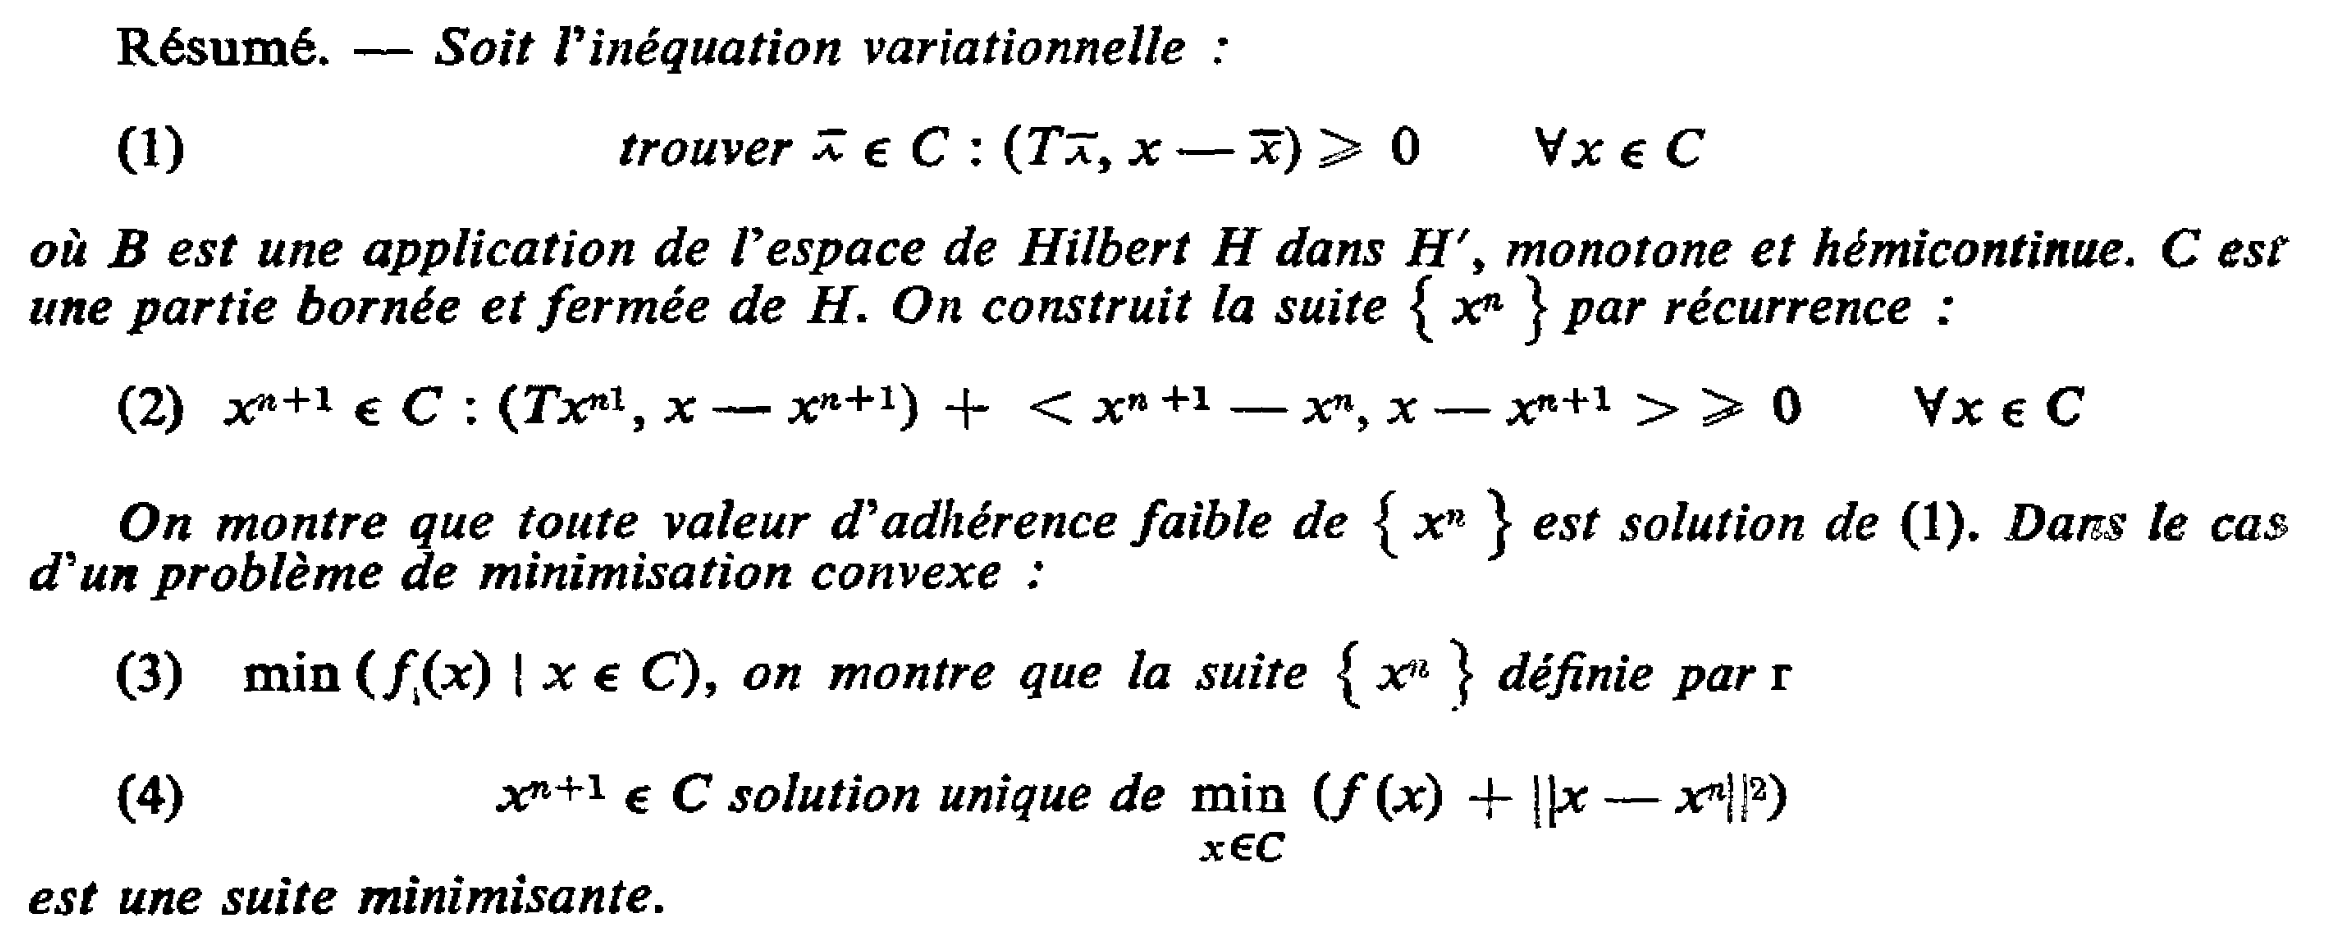
\includegraphics[height=1.25in,keepaspectratio]{figures/bmartinet_1970_summary.png}
\end{center}}
\visible<2->{
Rockafellar (1976), G\"uler (1991): Generalizations and main convergence statements. }
\end{beamercolorbox}}   \vspace{3ex}
\end{frame}
 

\begin{frame}\frametitle{Application to Obstacle Problem}
 \begin{beamercolorbox}[rounded=true, shadow=true, wd=\textwidth]{block body}
 	Applying this idea to the Obstacle Problem leads to the variational inequality:
	\begin{equation*}
%	\label{eq:L2ProxVI}
		\int_\Omega
		\nabla( (1+\alpha)u - u^{k}) \cdot \nabla w
		\dd x
		+
		\int_\Omega (u-u^{k}-\alpha f) w  \dd x
		\geq
		0
		~\fa w \in K-u,\quad \alpha > 0
	\end{equation*}
	But this is \alert{as difficult to solve as} the original VI!
 \end{beamercolorbox}
 \visible<2->{
 \begin{beamercolorbox}[rounded=true, shadow=true, wd=\textwidth]{block title}\centering
 The idea to use a regularization that includes information from the previous iterate $u^{k}$ is similar to AL (where we used $\lambda^{k}$).
 \end{beamercolorbox}}
 \visible<3->{
  \begin{beamercolorbox}[rounded=true, shadow=true, wd=\textwidth]{block body}
But the regularization
\[
u \mapsto \frac{1}{2\alpha} \| u - u^{k} \|^2_{H^1}
\]
is essentially \alert{useless}. There are, however, bivariate functions that behave similarly.
 \end{beamercolorbox}}
\end{frame}

 \begin{frame}\frametitle{Alternative Regularizations}
 \visible<1->{
  \begin{minipage}{0.67\linewidth}
\begin{beamercolorbox}[rounded=true, shadow=true, wd=\textwidth]{block body}
L.M. Bregman (1967): \visible<2->{Given a \alert{distance-generating functions} $R$,
the associated \alert{Bregman distance} measures the linearization error of $R$:
\begin{equation*}
%\label{eq:BregmanDivergence}
D_R(a, b) := R(a) - R(b) - \nabla R(b) \cdot (a-b),
\end{equation*}
for all $a \in \mathop{\text{dom}} R,~b \in \mathop{\text{int}} \mathop{\text{dom}} R$.}
\end{beamercolorbox}
\end{minipage}\hfill
\begin{minipage}{0.3\linewidth}
 \begin{figure}
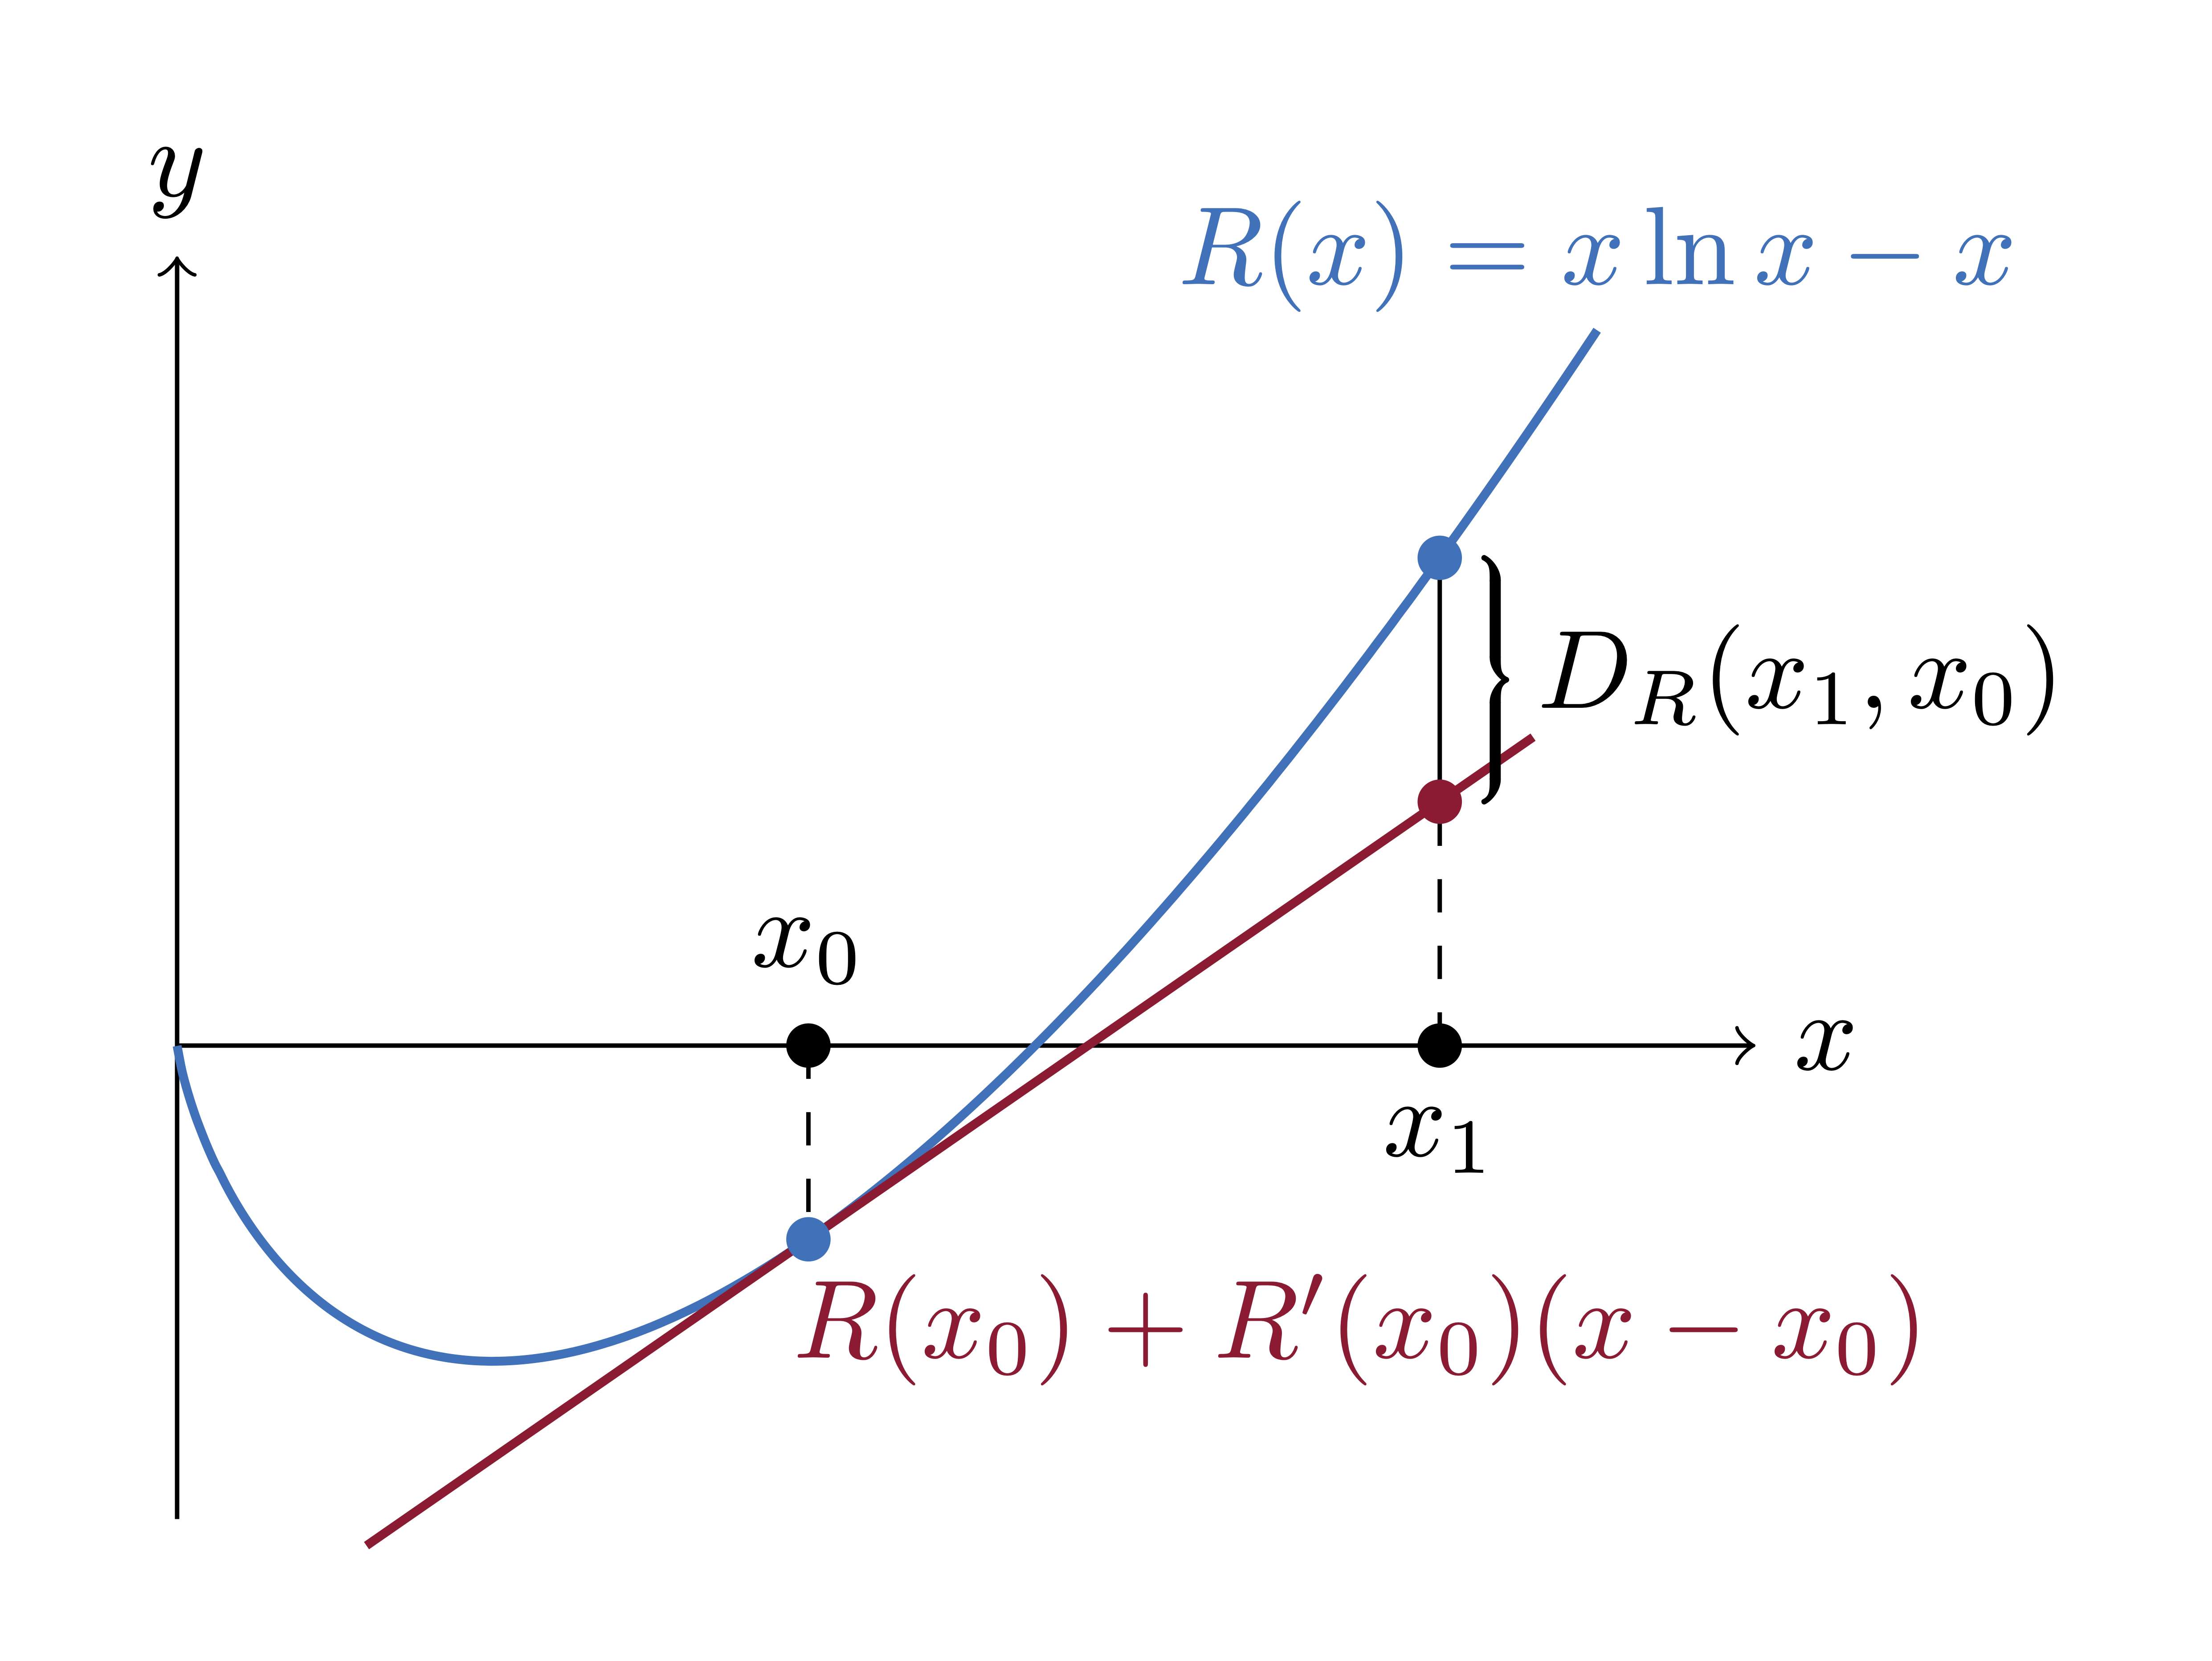
\includegraphics[height=1.25in,keepaspectratio]{figures/Bregman.png}
\end{figure}
\end{minipage}}

\visible<3->{
\begin{beamercolorbox}[rounded=true, shadow=true, wd=\textwidth]{block title}
Y. Censor \& S.A. Zenios (1992): Invention of the \textbf{Bregman Proximal Point Method}: Generate a sequence $\{u^k\}$\vspace{-2ex}
\[
u^{k+1} \in \mathrm{argmin}_{u \in V} \left\{J(u) + \frac{1}{\alpha^{k}} D(u,u^{k}) \right\}\quad \text{for}\quad \{\alpha^k\},\; \alpha^k > 0.
\]
G. Chen \& M. Teboulle (1993): Convergence proof based on G\"uler (1991).
\end{beamercolorbox}}
\end{frame}
 
  \begin{frame}\frametitle{Shannon Entropy \& Kullback-Leibler}
 \visible<1->{
  \begin{minipage}{0.67\linewidth}
\begin{beamercolorbox}[rounded=true, shadow=true, wd=\textwidth]{block body}
\visible<1->{The \alert{Shannon entropy} (C. Shannon (1948)) $R: \mathbb R_+ \to \mathbb R$:
\begin{equation*}
%\label{eq:GeneralizedShannonEntropy}
R(a) = a  \ln a  - a, %\text{ with } \nabla R^*(a^\ast) = \phi_1 + \exp{a^\ast},
\end{equation*}
yields
\[\aligned
D_{R}(a,b) 
%&= a \ln a - a - (b \ln b - b + (\ln b + 1 - 1)(a-b))\\
&= a \ln \frac{a}{b} - (a- b)
\endaligned
\]
}
for all $a \in \mathop{\text{dom}} R = \mathbb R_+,~b \in \mathop{\text{int}} \mathop{\text{dom}} R = \mathbb R_{++}$.
\end{beamercolorbox}}
\end{minipage}\hfill
\begin{minipage}{0.3\linewidth}
 \begin{figure}
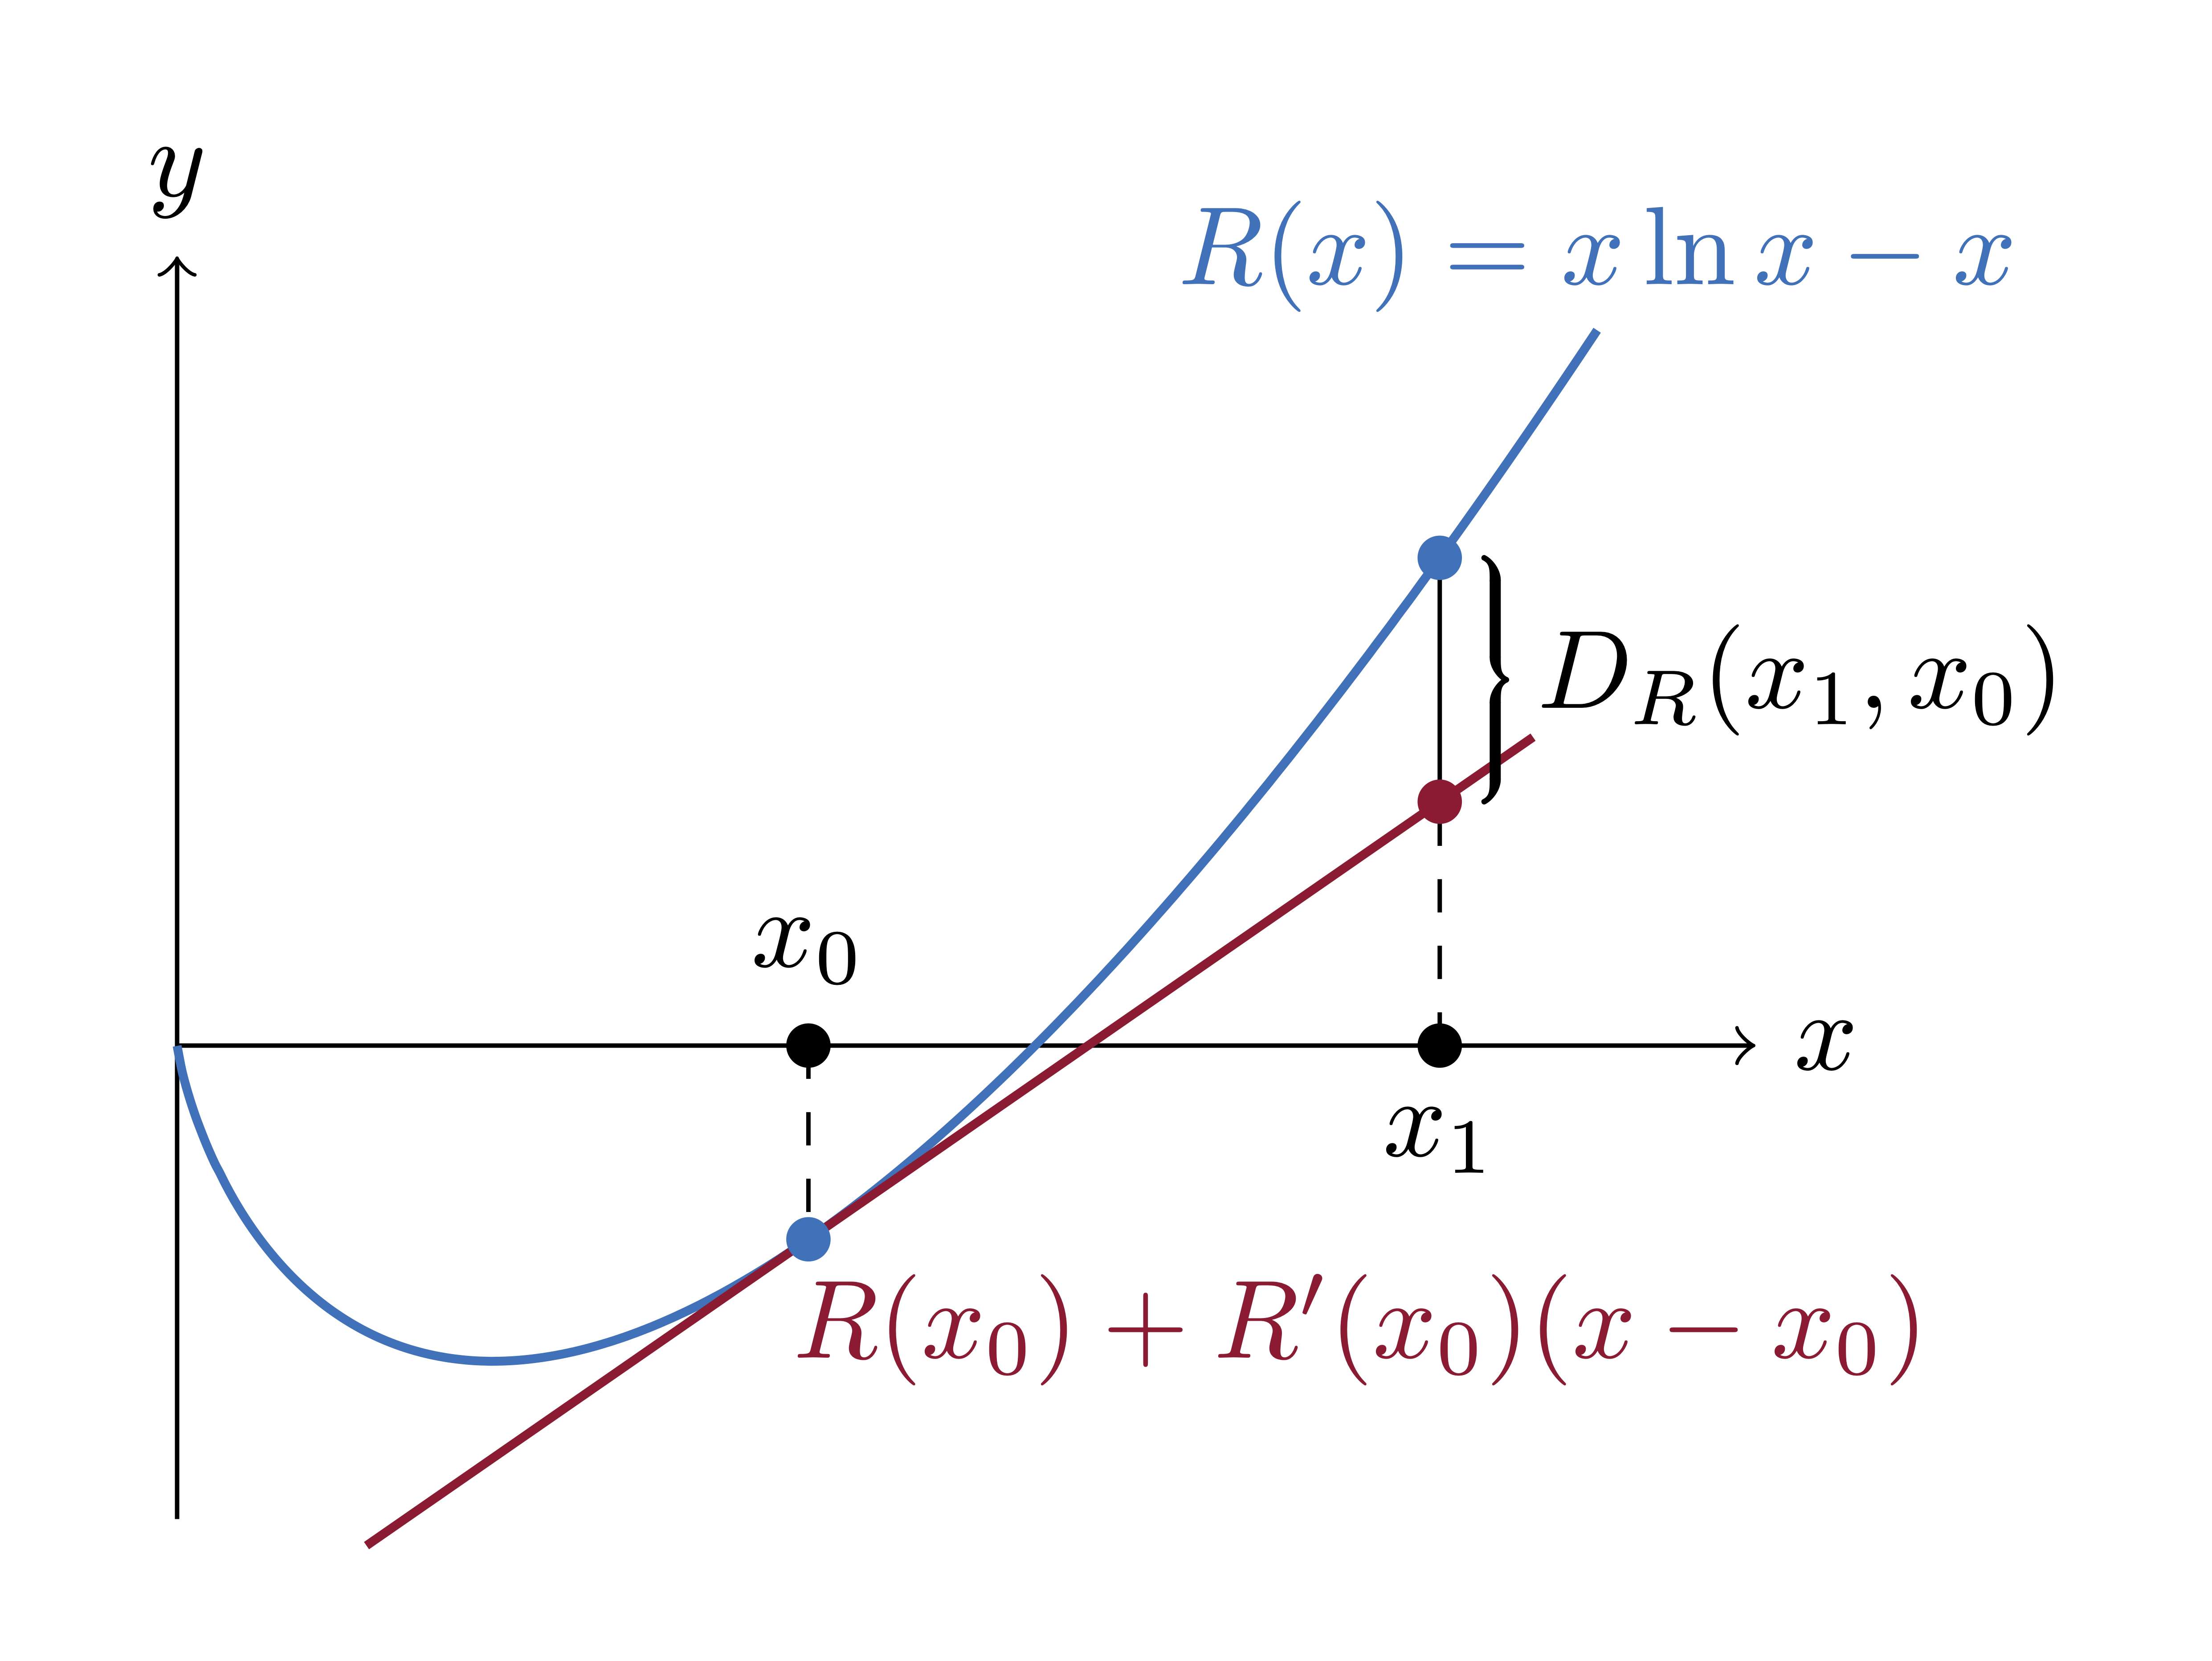
\includegraphics[height=1.25in,keepaspectratio]{figures/Bregman.png}
\end{figure}
\end{minipage}

%\visible<2->{
%\begin{beamercolorbox}[rounded=true, shadow=true, wd=\textwidth]{block title}
%In other words, the Bregman divergence associated with the Shannon entropy is the well-known \textbf{Kullback-Leibler divergence} (Kullback \& Leibler (1951)).
%\end{beamercolorbox}}
 \end{frame}
 
   \begin{frame}\frametitle{Return to the Obstacle Problem}
  \begin{minipage}{0.68\linewidth}
\begin{beamercolorbox}[rounded=true, shadow=true, wd=\textwidth]{block body}
 Given $\alpha > 0$, and a previous iterate $v > \varphi$, we consider:
 \begin{equation*}\aligned
 	L(u,v,\alpha)
 	&=
 	\frac{1}{2}\| \nabla u \|^2 - (f,u)\\
	&\hspace{8ex}+
	\frac{1}{\alpha}\int_{\Omega} (u - \varphi) \ln \left(\frac{u - \varphi}{v - \varphi}\right) - (u - v)\dd x
 	\endaligned
 \end{equation*}
 Set $L(u,v,\alpha) = +\infty$ if $u < \varphi$ on a set of positive measure.
\end{beamercolorbox}
\end{minipage}\hfill
\begin{minipage}{0.3\linewidth}
 \begin{figure}
% \resizebox{0.3\textwidth}{0.25\textwidth}{%
  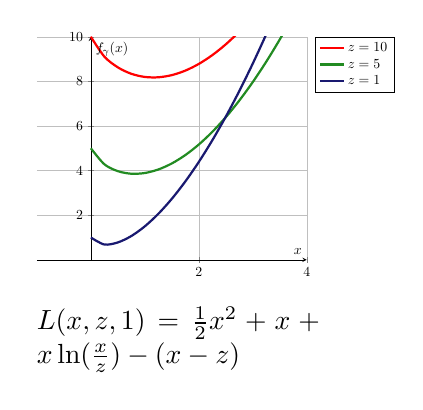
\begin{tikzpicture}[scale=0.5]
    \begin{axis}[
        axis lines=middle, % Draw axes through the origin
        xlabel=$x$,
        ylabel=$f_\gamma(x)$,
        xmin=-1, xmax=4, % Adjust x-range as needed
        ymin=-0.05, ymax=10, % Adjust y-range as needed
        grid=both, % Add a grid
        grid style={line width=.1pt, draw=gray!10}, % Style the grid lines
        major grid style={line width=.2pt,draw=gray!50}, % Style major grid lines
        xtick distance=2, % Tick marks every 1 unit on x-axis
        ytick distance=2, % Tick marks every 1 unit on y-axis
        % Add a legend
        legend pos=outer north east, % Position the legend
        legend cell align=left,
        no markers, % Don't put markers on the plots
    ]

    % Define the function with a placeholder for c
    % We use 'max(0,x)^2' for the (x)^2 part, and then multiply by c
    % PGFPlots works with degrees, so we need to be careful with functions that are not trigonometric.
    % max(0, x) is directly supported.


    \addplot[domain=-2:4, Red, ultra thick, smooth] {0.5*x^2 + 1*x  + (x * ln(x/10) - (x-10))/ 1};
    \addlegendentry{$z=10$};
    % Plot for c = 0.5
    \addplot[domain=-2:4, ForestGreen, ultra thick,smooth] {0.5*x^2 + 1*x   + (x * ln(x/5) - (x-5))/ (1)};
    \addlegendentry{$z=5$};

    % Plot for c = 1
    \addplot[domain=-2:4, MidnightBlue, ultra thick, smooth] {0.5*x^2 + 1*x +  (x * ln(x/1) - (x-1)) / (1)};
    \addlegendentry{$z=1$};

    % Plot for c = 2
%    \addplot[domain=-2:4, BurntOrange, ultra thick] {0.5*x^2 + 1*x  - x + 50.0 * max(0,-x)^2 * 0.5};
%    \addlegendentry{$\gamma=50$};
	
    \end{axis} \node[text width=4cm, align=left] at (4,-2) { $L(x,z,1) =\frac{1}{2} x^2 + x + x \ln(\frac{x}{z}) - (x-z)$};
\end{tikzpicture}
%}
%\caption{\scriptsize Plot of $L(x,\lambda,\gamma) =\frac{1}{2} x^2 + x -\lambda + \gamma\max\{0,-x\}^2$ with $\lambda = 0.5$}
  \label{fig:tikz-example}
\end{figure}
\end{minipage}\vspace{-3ex}\visible<2->{
 \begin{beamercolorbox}[rounded=true, shadow=true, wd=\textwidth]{block title}
Observation 1: We do not need to change $\alpha$ to move closer to the true solution.\medskip

Observation 2: Similar to IP, there is a logarithm in the regularization term.
 \end{beamercolorbox}}\hfill   
  \end{frame}
 
 \begin{frame}\frametitle{Properties of the Entropy Functional\footnote{\tiny Keith and Surowiec (2024) Thm.\ 4.1, Cor.\ 4.2. $L^p_+(\Omega) : = \left\{v \in L^p(\Omega) : v \ge 0 \right\}$}}
 {\scriptsize
\begin{minipage}{0.48\linewidth}
\begin{theorem}
Define $S : L^p(\Omega) \to \overline{\mathbb R}$, $p \in [1,\infty]$ by
\[
S(u) = \left\{
\begin{array}{cc}
\int_{\Omega} u \ln u - u \dd x, & \text{ if } u \in L^p(\Omega),\\
+\infty, & \text{ else.}
\end{array}
\right.
\]\visible<2->{
$p \in [1,\infty] \Rightarrow$ $S$ is strictly convex and l.s.c.\\}

\visible<3->{$p \in (1,\infty] \Rightarrow$ $S$ is continuous on $L^p_+(\Omega)$\\}

\visible<4->{$p = \infty \Rightarrow$ $S$ is cont. Fr\'echet diff. on $\mathrm{int}\, L^{\infty}_+(\Omega)$.}
\end{theorem}
\end{minipage}\hfill \visible<5->{
\begin{minipage}{0.48\linewidth}
\begin{theorem}[continued]\visible<5->{
For all $u \in \mathrm{int}\, L^{\infty}_+(\Omega)$ and $v \in L^{\infty}(\Omega)$ we have
\[
\langle S'(u), v \rangle = \int_{\Omega} v \ln u \, \dd x.
\]}\visible<6->{
Moreover, $\| S'(u) \|_{(L^{\infty}(\Omega))^*} = \| \nabla S(u) \|_{L^1(\Omega)}$ where
\[
\nabla S(u) = \ln u \in L^{\infty}(\Omega)
\]}\visible<7->{
is the unique primal representation of $S'(u)$ and 
\[
(\nabla S(u), v) = \langle S'(u) , v \rangle
\]
for all $u \in  \mathrm{int}\, L^{\infty}_+(\Omega)$ and $v \in L^1(\Omega)$.}
\end{theorem}
\end{minipage}}
}
 \end{frame}
 
  \begin{frame}\frametitle{The Entropic Poisson Equation\footnote{\tiny Keith and Surowiec (2024) Thm.\ 4.7, Cor.\ 4.9}}
 {\scriptsize
\begin{minipage}{0.48\linewidth}
\begin{theorem}
Assume $\Omega \subset \mathbb R^n$ is an open, bounded Lipschitz domain, $n \ge 1$, and 
$
K = \left\{v \in H^1_g(\Omega) \left| v \ge 0 \right.\right\}
$
where $g \in H^1(\Omega) \cap C(\overline{\Omega})$ and $\inf_{x \in \partial \Omega} g(x) > 0$.\medskip

\visible<2->{
Moreover, assume $f \in L^{\infty}(\Omega)$ and $w \in \mathrm{int}\, L^{\infty}_+(\Omega)$ and set 
$D(u,w) := S(u) - [S(w) + S'(w)(u-w)]$.}\medskip

\visible<3->{Then the optimization problem
\[
\min_{u \in K}\{J(u) + \frac{1}{\alpha} D(u,w)\}
\]
has a \alert{unique solution $u \in H^1_g(\Omega) \cap \mathrm{int}\, L^{\infty}_+(\Omega)$}.}
\end{theorem}
\end{minipage}\hfill \visible<4->{
\begin{minipage}{0.48\linewidth}
\begin{theorem}[continued]
In addition, $u$ satisfies the following \alert{Entropic Poisson Equation}
\[
-\alpha \Delta u + \ln u = \alpha f + \ln w;
\]
understood in $H^{-1}(\Omega)$.
\end{theorem}
\visible<5->{
\begin{beamercolorbox}[rounded=true, shadow=true, wd=\textwidth]{block body}
The proof is nontrivial. The steps involve
\begin{itemize}
\item Existence/uniqueness in $H^1_g(\Omega)$ (Direct Method).
\item Proof that $u \in \mathrm{int}\, L^{\infty}_+(\Omega)$ (Truncation).
%\[
%\min\{g_{\rm min}, e^(-\|\ln(w) + \alpha f\|_{L^{\infty}})\} \le u \le \max\{g_{\rm max}, e^(\|\ln(w) + \alpha f\|_{L^{\infty}})\} 
%\]
\item Derivation of a VI in $H^1(\Omega) \cap L^{\infty}(\Omega)$.
\item Density argument to obtain variational \alert{equation}.
\end{itemize}
\end{beamercolorbox}}
\end{minipage}}
}
 \end{frame}
 
 \begin{frame}\frametitle{Entropic Poisson $\leftrightarrow$ Saddle Point}
  \visible<1->{
   \begin{beamercolorbox}[rounded=true, shadow=true, wd=\textwidth]{block body}
\visible<1->{We again have a \alert{singular elliptic PDE} (the Entropic Poisson equation):
\[
-\Delta u  + \frac{1}{\alpha}(\ln u - \ln w) = f
\]
This can be solved with Newton's method, but this \alert{does not work very well}. \medskip 
}

\visible<2->{
Introduce \alert{latent variables} $\psi := \ln u$ and $\widetilde{\psi} := \ln w$.\footnote{\tiny These are well-defined by the theory (in fact $\psi$ has the same regularity as $u$ Keith and Surowiec (2024) Prop.\ A.8.}}
\visible<3->{
%This transforms Entropic Poisson into a \alert{nonlinear saddle point problem} in $(u,\psi)$:
\vspace{-2ex}
\begin{equation}\label{eq:lvpp-spp-obstacle}
	\begin{aligned}
					\,-\alpha \Delta u + \alert{\psi}
					&=
					\alpha f + \alert{\widetilde{\psi}}
					~~ &&\text{in~} \Omega\,,
					\\
%					\visible<4->{\tikzmark{b} \text{guarantees feasibility!}\quad }\tikzmark{f}
					\alert{u
					-
					\exp(\psi)}
					&=
					0
					~~ &&\text{in~} \Omega\,,
					\\
					u
					&=
					g ~~ &&\text{on~} \partial\Omega\,.
				\end{aligned}
				\end{equation}}\vspace{-2.3ex}
\end{beamercolorbox}}   
  
%\begin{tikzpicture}[overlay,remember picture]
%    \draw[very thick, -Stealth]         ($({pic cs:b})+(1ex,1ex)$)
%        to [bend left, sloped, "text"]  ($({pic cs:f})+(1ex,+1em)$);
%    \end{tikzpicture}

\end{frame}

\begin{frame}\frametitle{Latent Variable Proximal Point\footnote{\tiny Keith and Surowiec (2024) Sec. 4.5}}
\begin{beamercolorbox}[rounded=true, shadow=true, wd=\textwidth]{block title}\centering
Recursively solving the saddle point problem and setting $w := u$ leads to the\\ \textbf{Latent Variable Proximal Point} (LVPP) algorithm. 
\end{beamercolorbox}

\visible<2->{
\begin{beamercolorbox}[rounded=true, shadow=true, wd=\textwidth]{block body}
\begin{equation}\label{eq:lvpp-spp-obstacle}
	\begin{aligned}
					\,-\alpha \Delta u + \alert{\psi}
					&=
					\alpha f + \alert{\widetilde{\psi}}
					~~ &&\text{in~} \Omega\,,
					\\
					\alert{u
					-
					\exp(\psi)}
					&=
					0
					~~ &&\text{in~} \Omega\,,
					\\
					u
					&=
					g ~~ &&\text{on~} \partial\Omega\,.
				\end{aligned}
				\end{equation}
\visible<3->{Discretizing \eqref{eq:lvpp-spp-obstacle} with a Galerkin method yields the \textbf{Proximal Galerkin}\footnote{\tiny Keith and Surowiec (2024)} (PG) method.} 
\end{beamercolorbox}
}
\visible<4->{
\begin{minipage}{0.48\linewidth}
\begin{beamercolorbox}[rounded=true, shadow=true, wd=\textwidth]{block body}
Recall the \alert{major challenge} to ensure \alert{global feasibility} for discrete solution.
\end{beamercolorbox}
\end{minipage}
}
\visible<5->{
\begin{minipage}{0.48\linewidth}
\begin{beamercolorbox}[rounded=true, shadow=true, wd=\textwidth]{block title}
Discrete solution $(u_h,\psi_h)$: $u_h \ge 0$ not guaranteed, but $\widetilde{u}_h := \exp(\psi_h) > 0$!
\end{beamercolorbox}
\end{minipage}
}
\end{frame}
 
 \subsection{First Numerical Experiments}
 
 \begin{frame}\frametitle{Experiments}
\begin{center}
\Large How does PG behave over various meshes and polynomials degrees?
\end{center}
\end{frame}

\begin{frame}\frametitle{Experiments}
\begin{minipage}{0.55\linewidth}
\begin{beamercolorbox}[rounded=true, shadow=true, wd=\textwidth]{block body}
\visible<1->{$\Omega := \Omega_{\infty} = [-1,1]\times[-1,1] \subset \mathbb R^2$}

\visible<2->{Set $\lambda = 0$ and $g=u$, where %$u(x,y)$ is the smooth manufactured solution 
\begin{equation*}
\label{eq:Biactivity_SmoothManufacturedSolution}
	u(x,y)
	=
	\begin{cases}
		0 & \text{if~} x < 0\,,\\
		x^4 & \text{otherwise,}\\
	\end{cases}
%	\quad
	% \iff
%	\text{implied by}
%	% \impliedby
%	\quad
%	f(x,y)
%	=
%	\begin{cases}
%		0 & \text{if~} x < 0\,,\\
%		-12x^2 & \text{otherwise.}\\
%	\end{cases}
\end{equation*}
$f = -(\partial^2_{xx} u + \partial^2_{yy} u)$.}
\end{beamercolorbox}
\visible<3->{
\begin{beamercolorbox}[rounded=true, shadow=true, wd=\textwidth]{block title}
Strict complementarity fails on $[-1,0] \times [-1,1]$.
\end{beamercolorbox}
}
\end{minipage}%
\visible<2->{
\begin{minipage}{0.3\linewidth}
\centering
\begin{figure}
	\centering
	\begin{tikzpicture}
		\node at (-3.35,0.5) {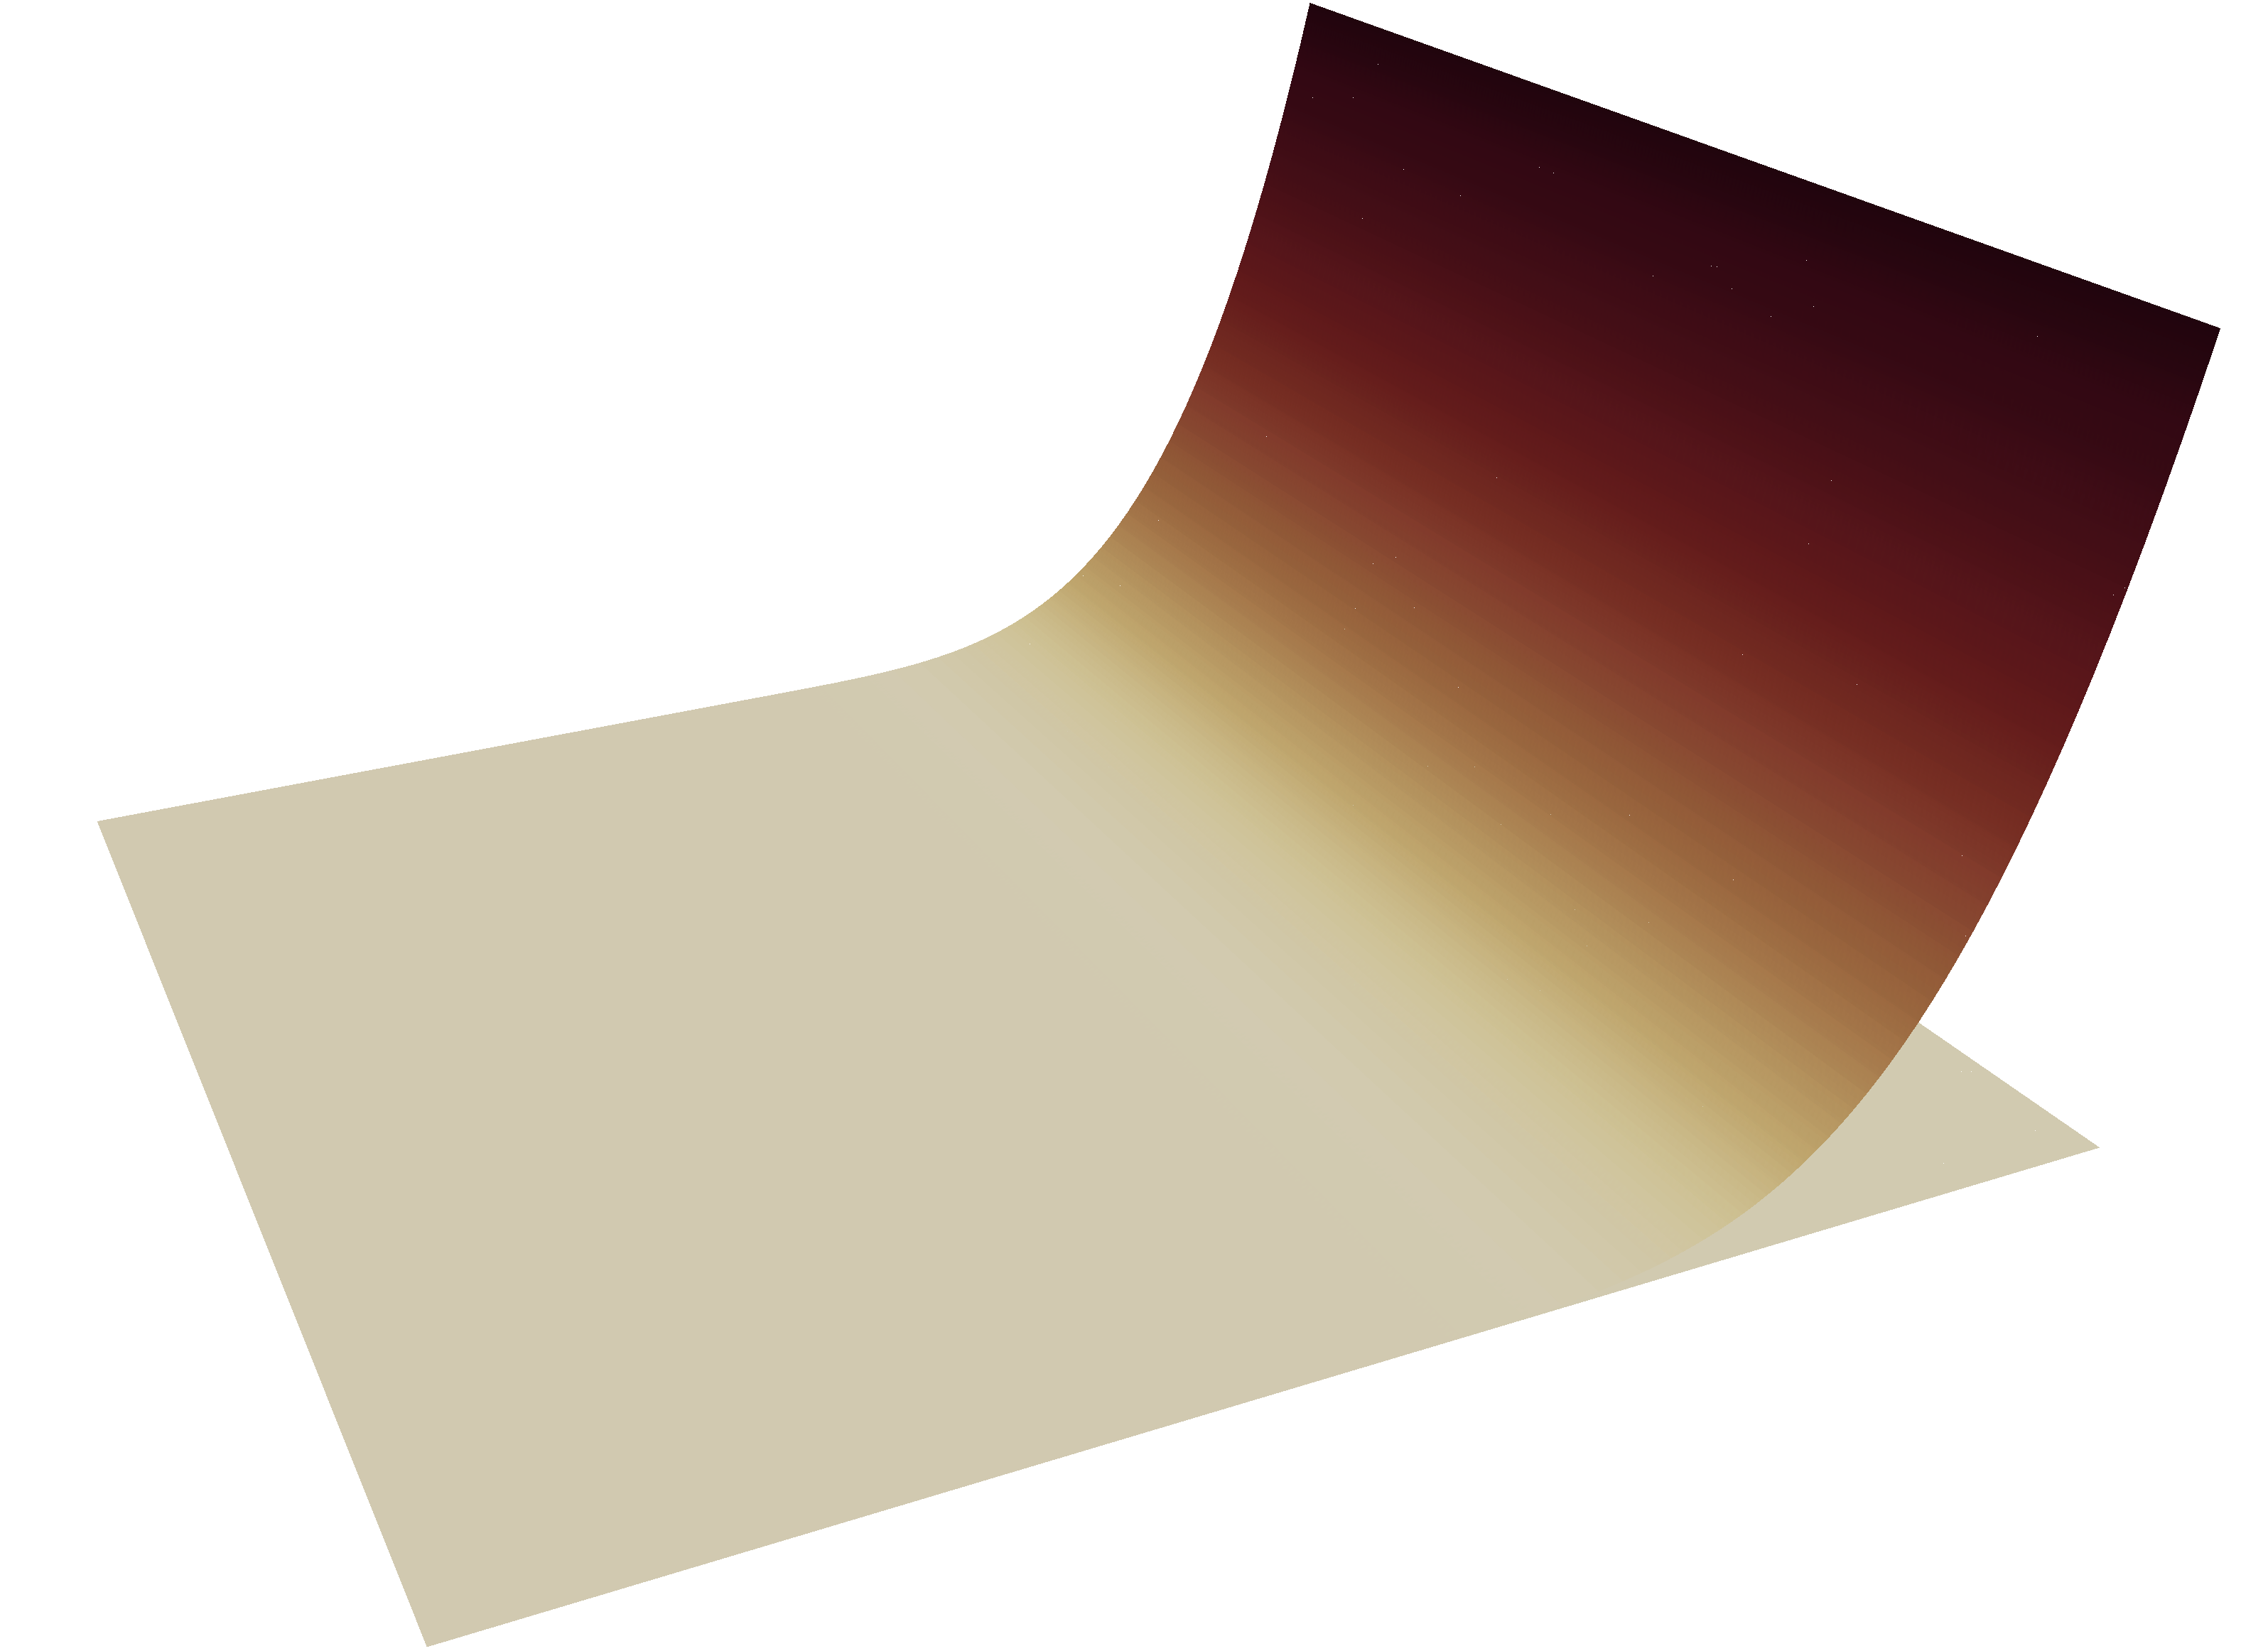
\includegraphics[height=1.5in]{figures/ObstacleExperiment1.png}};
		%\node at (3.25,0.4) {
		%	   \includegraphics[clip=true, trim= 0 0 0.35cm 0, height=2.1in]{Figures/tikz/FEniCS_plots/example0/example0_ConvergenceRate.pdf}
		%};
	    \node at (-0.5,0.4) {\includegraphics[height=2cm]{figures/colorbar0.pdf}};
	    \node at (-2.2,-1.35) {\scriptsize $
	    	u(x,y)
	    	=
	    	\begin{cases}
	    		0 & \text{if~} x < 0\\
	    		x^4 & \text{otherwise}\\
	    	\end{cases}
	    $};
    \end{tikzpicture}
\end{figure}
\end{minipage}}

\visible<4->{
\begin{beamercolorbox}[rounded=true, shadow=true, wd=\textwidth]{block title}
%Proximal point is a (slow) fixed point method if $\alpha$ is left fixed.\smallskip

We choose $\left\{\alpha_k\right\}$ with $\alpha_1 = 1$ and $\alpha_k$ increasing to a maximum value of $10^{10}$
\end{beamercolorbox}
}
\hypertarget{example_1_alpha}{}
 \hyperlink{target_alpha}{\beamerbutton{Go to choice of $\alpha$}}
  \hyperlink{target_fem}{\beamerbutton{Go to choice FE spaces}}
% \hypertarget{example_1}{}
% \hyperlink{target}{\beamerbutton{Go to Finite Element Spaces}}
%  \hyperlink{target_alg}{\beamerbutton{Go to Algorithm and Convergence}}
\end{frame}



\begin{frame}\frametitle{Experiment 1: Results}

\begin{table}
\centering
\tiny
\renewcommand{\arraystretch}{1.3}
\begin{tabular}{ |c|c|c|c|c|c|c| }
 \hhline{|>{\arrayrulecolor{white}}-->{\arrayrulecolor{black}}|-----|}
 \multicolumn{2}{c|}{} & \multicolumn{5}{c|}{\cellcolor{lightgray!15} \small\raisebox{5pt}{\vphantom{f}} Progress of the iterates $\|u_h^{k} - u_h^{k-1}\|_{H^1(\Omega_\infty)}$ for various $h$ and $p$}\\[3pt]
 \hhline{|>{\arrayrulecolor{white}}-->{\arrayrulecolor{black}}|-----|}
 \multicolumn{2}{c|}{}& \multicolumn{3}{c|}{\cellcolor{lightgray!05} Polynomial degree $p = 1$} & \multicolumn{2}{c|}{\cellcolor{lightgray!10} Polynomial degree $p = 2$}\\
 \hline
 \rowcolor{lightgray!15}
 $k$ & $\alpha_{k}$ & $h_\infty/16$ & $h_\infty/32$ & $h_\infty/64$ & $h_\infty/16$ & $h_\infty/32$ \\
 \hline
\cellcolor{lightgray!05}   1 & \cellcolor{lightgray!01}   $1.0$              & $2.10\cdot 10^{0}$   & $2.10\cdot 10^{0}$   & $2.10\cdot 10^{0}$   & $2.10\cdot 10^{0}$   & $2.10\cdot 10^{0}$   \\
\cellcolor{lightgray!05}   2 & \cellcolor{lightgray!01}   $1.0$              & $6.45\cdot 10^{-1}$  & $6.45\cdot 10^{-1}$  & $6.45\cdot 10^{-1}$  & $6.45\cdot 10^{-1}$  & $6.45\cdot 10^{-1}$  \\
\cellcolor{lightgray!05}   3 & \cellcolor{lightgray!01}   $1.49$             & $1.73\cdot 10^{-1}$  & $1.73\cdot 10^{-1}$  & $1.73\cdot 10^{-1}$  & $1.73\cdot 10^{-1}$  & $1.73\cdot 10^{-1}$  \\
\cellcolor{lightgray!05}   4 & \cellcolor{lightgray!01}   $2.43$             & $1.10\cdot 10^{-1}$  & $1.10\cdot 10^{-1}$  & $1.10\cdot 10^{-1}$  & $1.10\cdot 10^{-1}$  & $1.10\cdot 10^{-1}$  \\
\cellcolor{lightgray!05}   5 & \cellcolor{lightgray!01}   $5.35$             & $7.76\cdot 10^{-2}$  & $7.77\cdot 10^{-2}$  & $7.77\cdot 10^{-2}$  & $7.77\cdot 10^{-2}$  & $7.77\cdot 10^{-2}$  \\
\cellcolor{lightgray!05}   6 & \cellcolor{lightgray!01}   $1.64\cdot 10^{1}$ & $4.76\cdot 10^{-2}$  & $4.77\cdot 10^{-2}$  & $4.77\cdot 10^{-2}$  & $4.77\cdot 10^{-2}$  & $4.77\cdot 10^{-2}$  \\
\cellcolor{lightgray!05}   7 & \cellcolor{lightgray!01}   $8.50\cdot 10^{1}$ & $2.24\cdot 10^{-2}$  & $2.25\cdot 10^{-2}$  & $2.25\cdot 10^{-2}$  & $2.25\cdot 10^{-2}$  & $2.25\cdot 10^{-2}$  \\
\cellcolor{lightgray!05}   8 & \cellcolor{lightgray!01}   $9.35\cdot 10^{2}$ & $5.82\cdot 10^{-3}$  & $5.84\cdot 10^{-3}$  & $5.85\cdot 10^{-3}$  & $5.85\cdot 10^{-3}$  & $5.85\cdot 10^{-3}$  \\
\cellcolor{lightgray!05}   9 & \cellcolor{lightgray!01}   $3.17\cdot 10^{4}$ & $6.04\cdot 10^{-4}$  & $6.07\cdot 10^{-4}$  & $6.07\cdot 10^{-4}$  & $6.07\cdot 10^{-4}$  & $6.07\cdot 10^{-4}$  \\
\cellcolor{lightgray!05}  10 & \cellcolor{lightgray!01}   $5.85\cdot 10^{6}$ & $1.80\cdot 10^{-5}$  & $1.81\cdot 10^{-5}$  & $1.81\cdot 10^{-5}$  & $1.81\cdot 10^{-5}$  & $1.81\cdot 10^{-5}$  \\
\cellcolor{lightgray!05}  11 & \cellcolor{lightgray!01}   $1\cdot 10^{10}$   & $9.41\cdot 10^{-8}$  & $9.47\cdot 10^{-8}$  & $9.49\cdot 10^{-8}$  & $9.50\cdot 10^{-8}$  & $9.50\cdot 10^{-8}$  \\
\cellcolor{lightgray!05}  12 & \cellcolor{lightgray!01}   $1\cdot 10^{10}$   & $2.10\cdot 10^{-12}$ & $2.00\cdot 10^{-12}$ & $1.96\cdot 10^{-12}$ & $1.92\cdot 10^{-12}$ & $1.95\cdot 10^{-10}$ \\
 \hline
 \rowcolor{lightgray!05}
 \multicolumn{2}{|c|}{\cellcolor{lightgray!15} Tot. linear solves} & $21$ & $20$ & $19$ & $19$ & $19$ \\
 \hline
\end{tabular}

%\caption{\label{tab:BiactivityMeshIndependence}
%Biactivity.
%Table of increments $\|u_h^{k} - u_h^{k-1}\|_{H^1(\Omega_\infty)}$ for various mesh sizes $h$ and polynomial orders $p$ using the triangular element $(\mathbb{P}_p\text{-bubble},\mathbb{P}_{p-1}\text{-broken})$ discretization.
%% of the biactive manufactured solution~\cref{eq:Biactivity_SmoothManufacturedSolution} on $\Omega = \Omega_\infty$.
%The initial degrees of freedom for $u_h$ and $\psi_h$ were set to zero at the beginning of each run.
%Between eight and ten Newton iterations performed by the PETSc Newton solver used for each initial subproblem solve and then only one Newton solve was used for each of the following subproblems.
%The convergence of the increments for each fixed $k$ and the boundedness of the number of linear solves indicates \emph{mesh-independence}.
%}
\end{table}
\begin{center}
 Remarkably, PG exhibits \alert{both mesh independence} and \alert{degree independence}!
\end{center}
\end{frame}

 \begin{frame}\frametitle{Other Proximal Methods from LVPP} 
  \begin{beamercolorbox}[rounded=true, shadow=true, wd=\textwidth]{block title}\centering
The iterates $u^k$, $\lambda^{k} = (\psi^k - \psi^{k+1})/\alpha_{k+1}$ converge like $O((\sum_{j=1}^k \alpha_j)^{-1/2})$.\footnote{\tiny Thm. 4.13 in Keith and Surowiec (2024) }
  \end{beamercolorbox}\hfill

\visible<2->{  
\begin{beamercolorbox}[rounded=true, shadow=true, wd=\textwidth]{block body}
The LVPP algorithm is \alert{agnostic} to the type of discretization, other \alert{proximal discretizations} are possible.
  \end{beamercolorbox}}
  
\visible<3->{
\begin{minipage}{0.7\linewidth}
\begin{beamercolorbox}[rounded=true, shadow=true, wd=\textwidth]{block body}
%\begin{figure}[c]{0.64\textwidth}
\centering
%\footnotesize
%\renewcommand{\arraystretch}{1.3}
\begin{tabular}{ |c| >{\centering}p{0.5cm}  >{\centering}p{0.5cm} >{\centering}p{0.5cm}  >{\centering}p{0.5cm}  >{\centering}p{0.5cm} >{\centering\arraybackslash}p{0.5cm}| }
 \hline
 \rowcolor{lightgray!10}
Mesh size $h$ & $2^{-1}$ & $2^{-2}$ & $2^{-3}$ & $2^{-4}$ & $2^{-5}$ & $2^{-6}$ \\
 \hline
\cellcolor{lightgray!02}  Finite Difference & 10 & 15 & 13 & 15 & 16 & 16  \\
\hline\hline
 \rowcolor{lightgray!10}
Degree $p$ & $8$ & $16$ & $24$ & $32$ & $40$ & $48$ \\
 \hline
\cellcolor{lightgray!02}  Spectral Method & 16 & 17 & 16 & 16 & 16 & 15 \\
 \hline
\end{tabular}\medskip

\scriptsize
%\caption{
Number of linear system solves for the proximal finite difference and spectral methods.
%}
%\label{fig:ObstacleExperiment_Discretizations}
%\end{figure}
\end{beamercolorbox}
\end{minipage}%
\begin{minipage}{0.3\linewidth}
 \centering
\begin{figure}
	\centering
	\begin{tikzpicture}
		\node at (-4.2,1.2) {\scriptsize 
	    	$u$};
		\node at (-3.35,0) {\includegraphics[height=1.25in]{../Part I/figures/obstacle_new.png}};
		\node at (-2.2,-1.35) {\scriptsize 
	    	$\varphi$};
    \end{tikzpicture}
\end{figure}
\end{minipage}
}
 \end{frame}

\section{The Latent Variable Proximal Point Method}

\begin{frame}[plain,c]
%\frametitle{A first slide}
\hfill
\begin{center}
\Huge What is really going on here?
\end{center}
\hfill
\end{frame}

%\begin{frame}{Overview}
%
%\tableofcontents
%\end{frame}


\subsection{Geometry Preserving Transformations}


\begin{frame}\frametitle{Bregman Proximal Point}
\only<1,2>{Abstractly speaking, we began with the optimization problem:}
\only<3>{The optimality conditions provide us with a variational inequality:}
\only<4>{Since the variational inequality does not reduce to a variational equation:}
\[
\only<1,2>{ \min_{u \in K} J(u)}
\only<3>{ \min_{u \in K} J(u) \quad \rightarrow \quad \text{Find } u \in K : J'(u)(v - u) \ge 0,\; \forall v \in K.}
\only<4>{\text{ Solve }\quad \min_{u \in K} J(u) \quad \text{ by recursively solving }  \quad \min_{u \in K} J(u) + \alpha^{-1} D(u,u_{\text{old}}) \quad \text{instead.}}
\]
\only<2,3>{
\begin{minipage}{0.5\textwidth}
\begin{beamercolorbox}[rounded=true, shadow=true, wd=\textwidth]{block body}
$V$: a reflexive Banach space,\smallskip

$K \subset V$: a closed convex set,\smallskip

$J$: a smooth coercive functional.
\end{beamercolorbox}
\end{minipage}
}
\only<4->{
\begin{minipage}{0.5\textwidth}
\begin{beamercolorbox}[rounded=true, shadow=true, wd=\textwidth]{block body}
$V$: a reflexive Banach space,\smallskip

$K \subset V$: a closed convex set,\smallskip

$J$: a smooth coercive functional,\smallskip

$D : K \times K \to \overline{\mathbb R}$ is a \alert{Bregman distance.}
\end{beamercolorbox}
\end{minipage}%
\begin{minipage}{0.5\textwidth}
\begin{figure}[h]
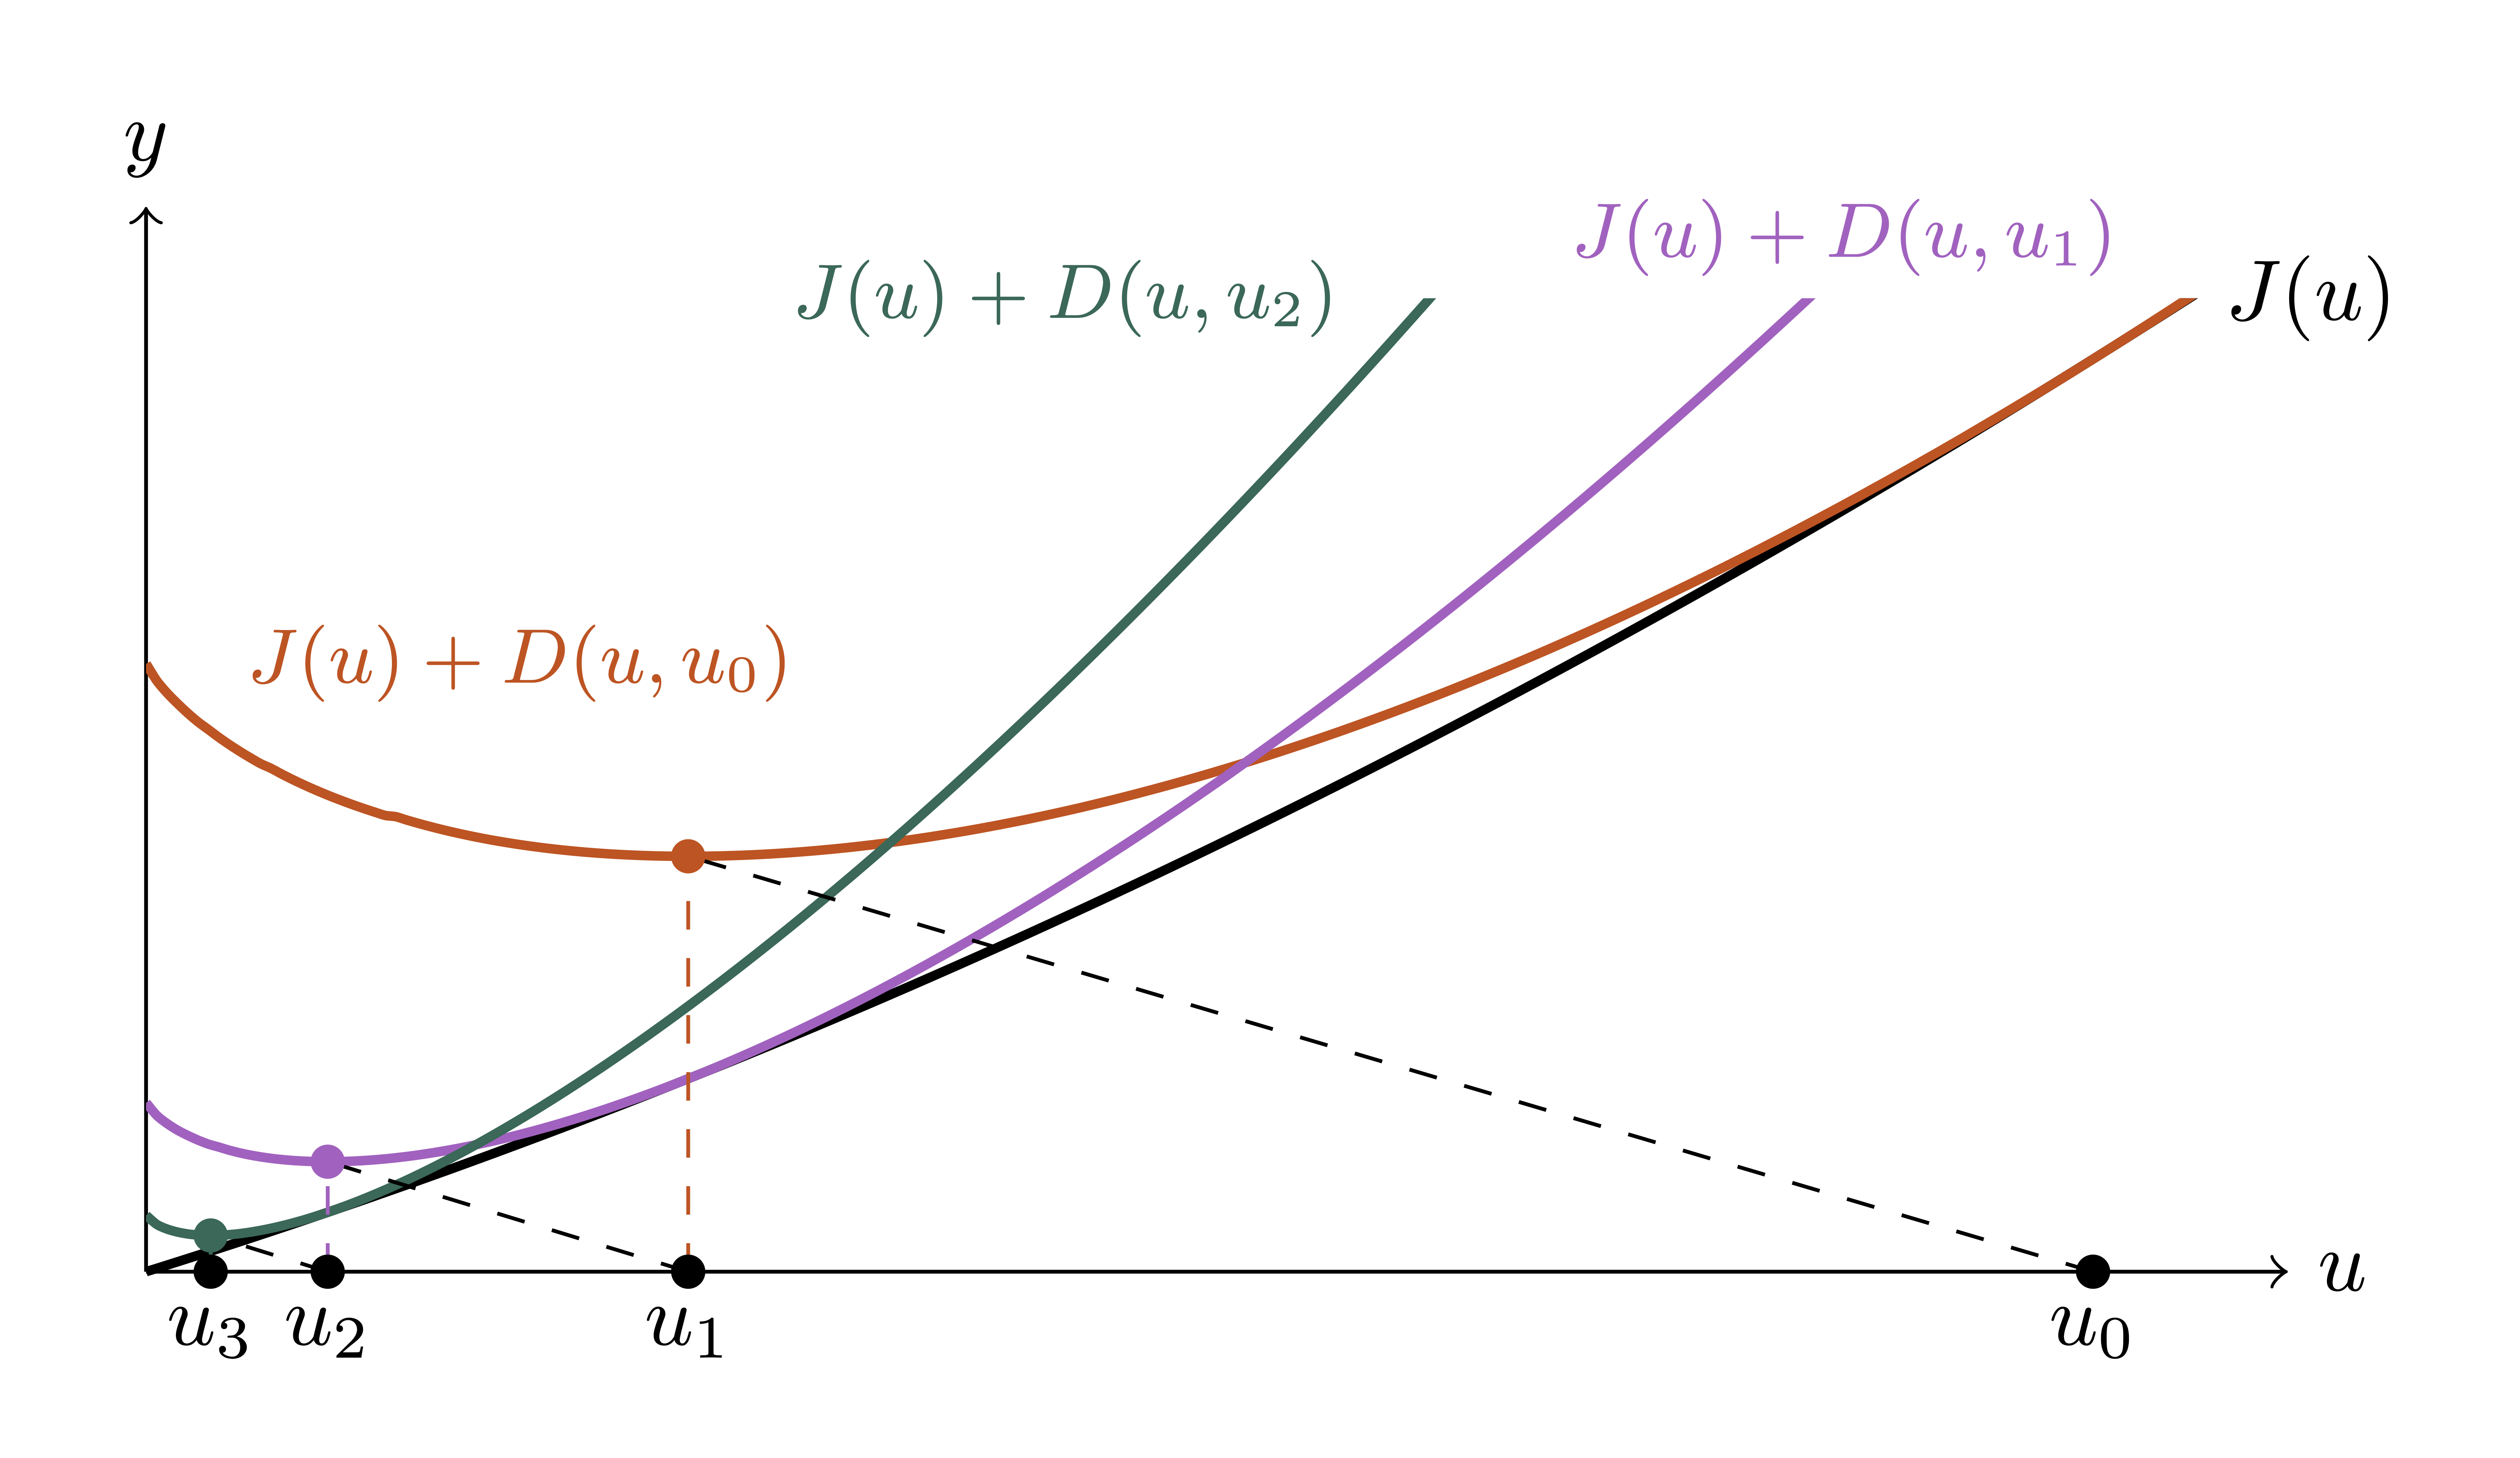
\includegraphics[width=0.8\linewidth]{figures/Prox.png}
\caption{Illustration of Bregman Proximal Point.} 
\end{figure}
\end{minipage}
}
\end{frame}

%\begin{frame}\frametitle{Bregman Distances}
%
%\begin{minipage}{0.5\linewidth}
%\begin{beamercolorbox}[rounded=true, shadow=true, wd=\textwidth]{block body}
%\visible<1->{Bregman distances/divergences are induced by \textbf{distance-generating functions} $R$.}\smallskip
%
%\visible<2->{They measure the linearization error of $R$:
%\begin{equation*}
%%\label{eq:BregmanDivergence}
%D_R(a, b) := R(a) - R(b) - \nabla R(b) \cdot (a-b),
%\end{equation*}
%for all $a \in \mathop{\text{dom}} R,~b \in \mathop{\text{int}} \mathop{\text{dom}} R$.}
%\end{beamercolorbox}
%\end{minipage}\visible<2->{
% \begin{minipage}{0.4\linewidth}
% \centering
%\begin{figure}[h]
%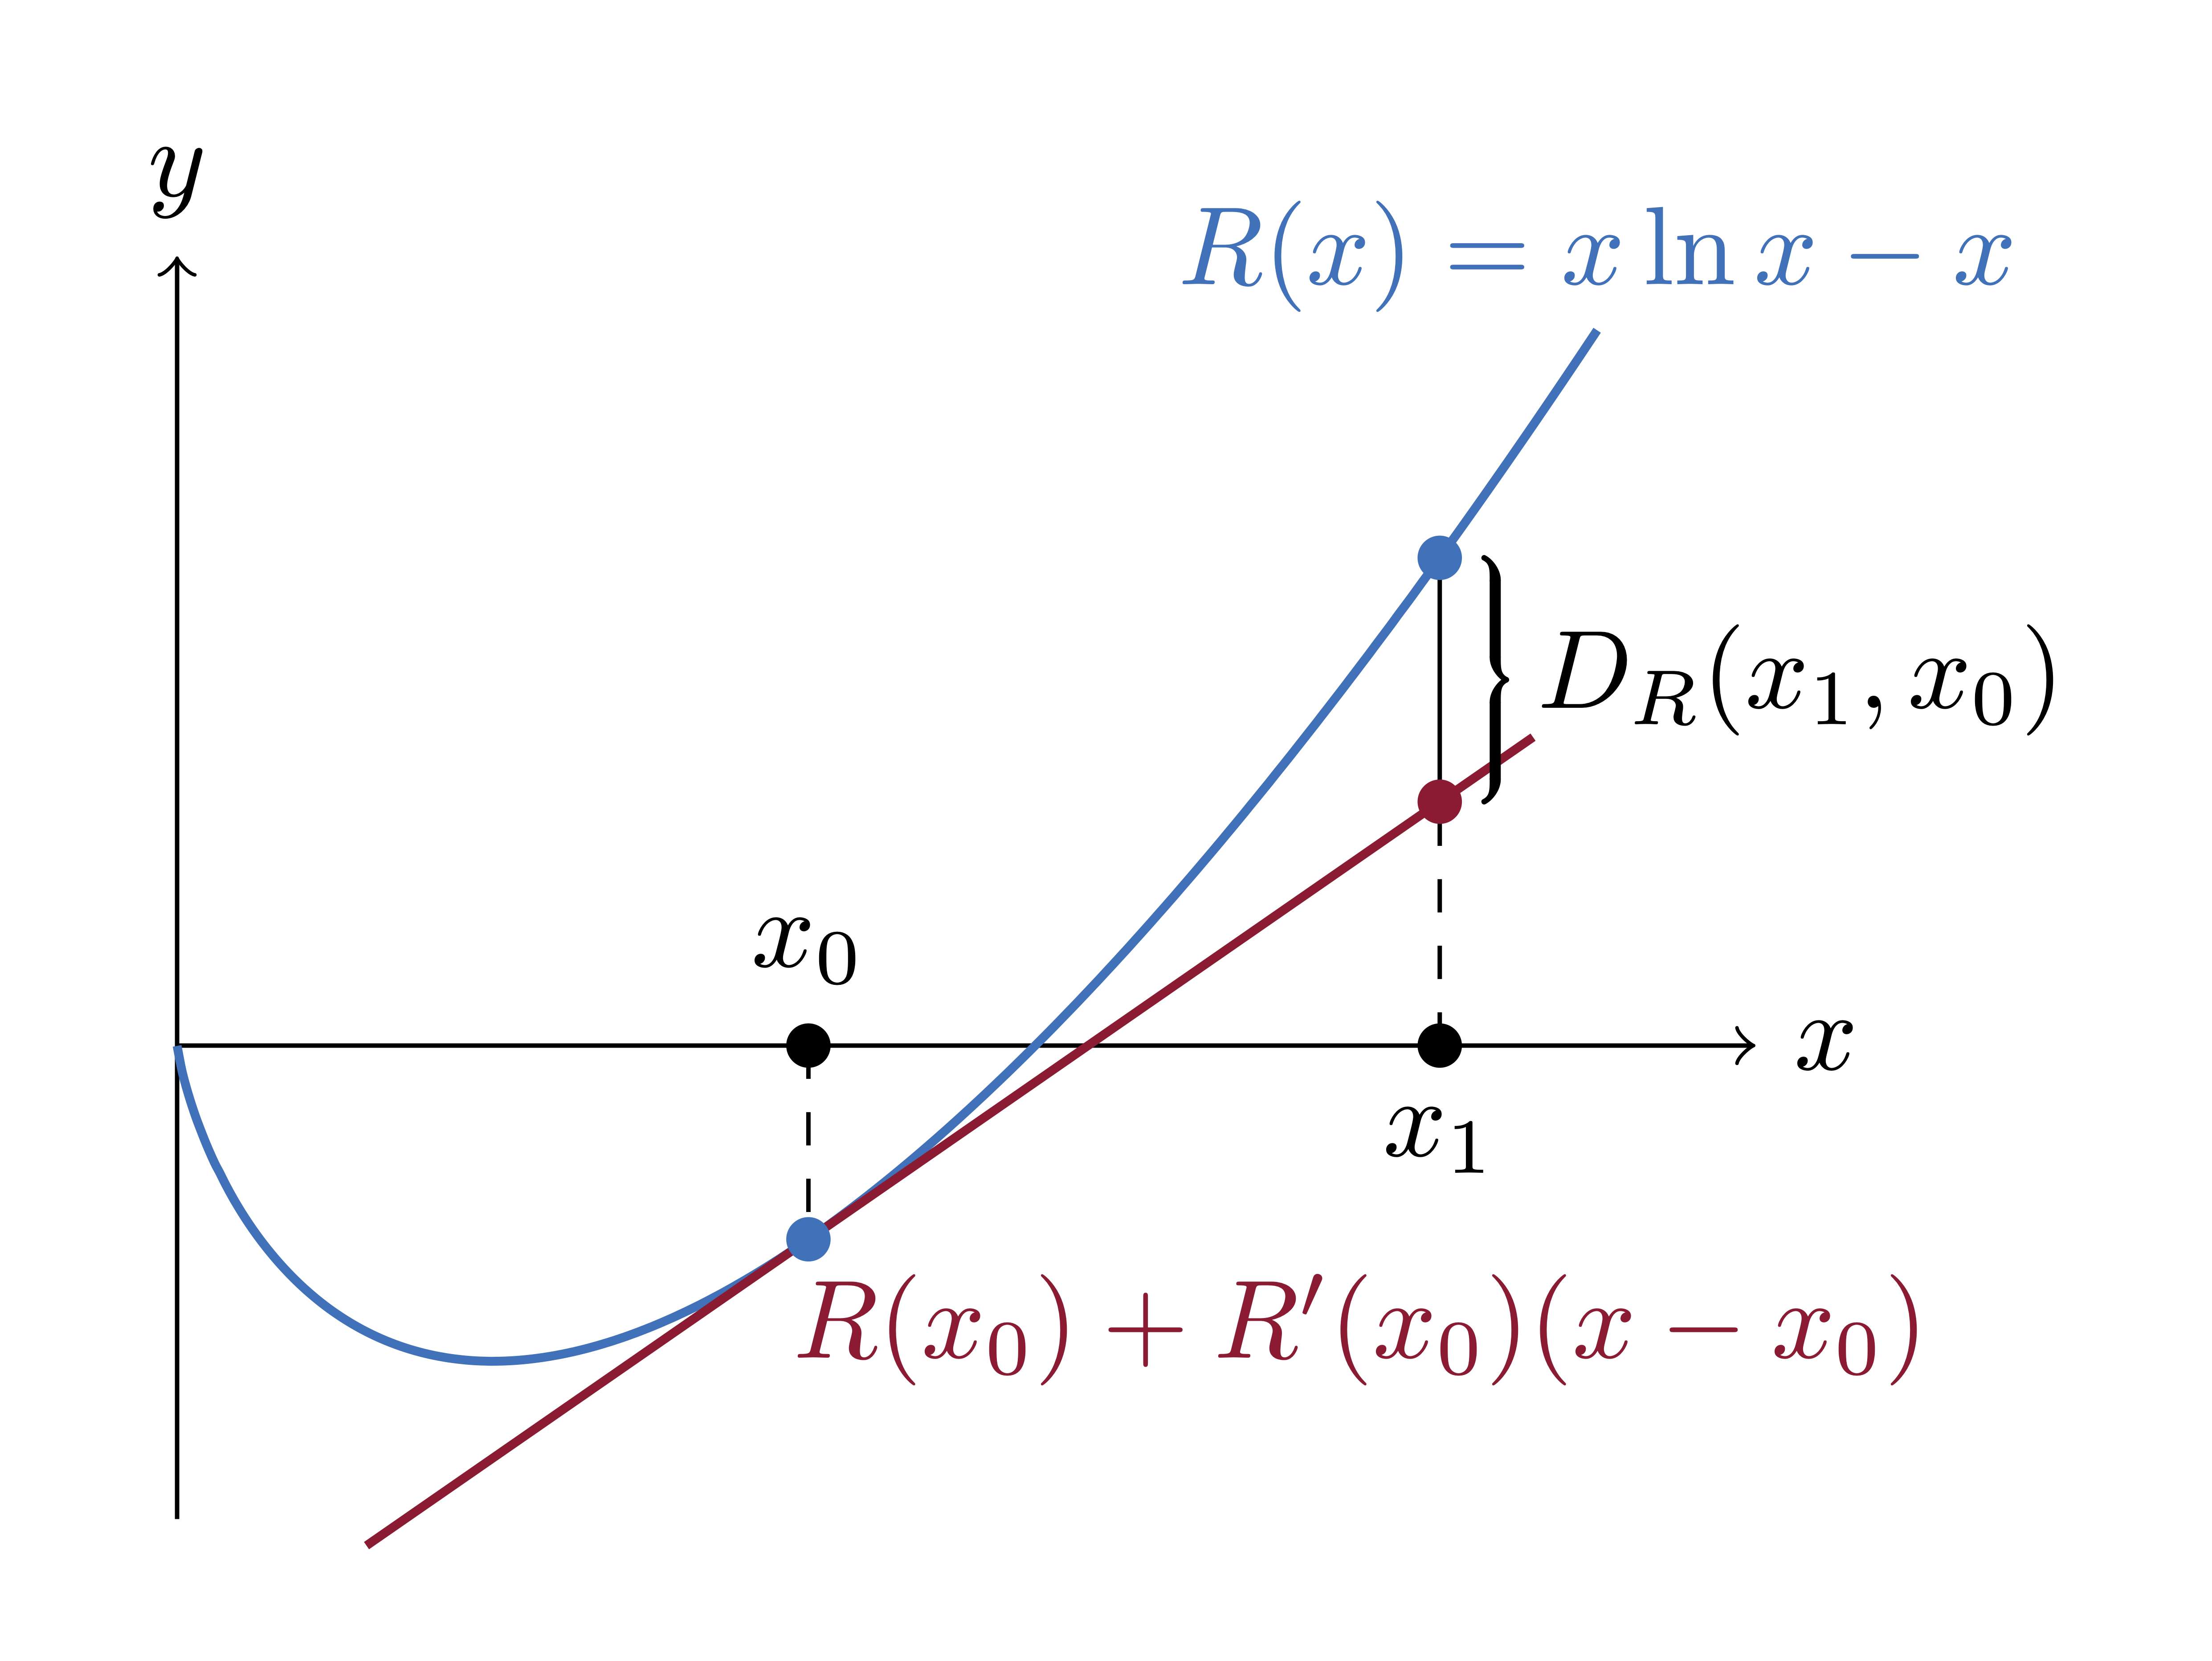
\includegraphics[width=0.8\linewidth]{figures/Bregman.png}
%\end{figure}}
%\visible<3->{
%\begin{beamercolorbox}[rounded=true, shadow=true, wd=\textwidth]{block title}
%They are very useful when the geometry of $K$ can be encoded in $\mathop{\text{dom}} R$.
%\end{beamercolorbox}}
%\end{minipage}
%\end{frame}

\begin{frame}\frametitle{Observations}
\begin{beamercolorbox}[rounded=true, shadow=true, wd=\textwidth]{block title}
\centering
 \visible The abstract LVPP framework lies in the construction of the Bregman divergence.
\end{beamercolorbox}

\visible<2->{
\begin{beamercolorbox}[rounded=true, shadow=true, wd=\textwidth]{block body}
Minimal properties of $R$:
\begin{itemize}
\item \visible<2->{Proper: $R > -\infty$ and there exists $a \in \mathbb R^n$ such that $R(a) < +\infty$.\smallskip}

\item \visible<3->{Convex: $R(\lambda a + (1-\lambda)b) \le \lambda R(a) + (1-\lambda) R(b) \quad \forall a,b \in \mathbb R^n, \forall \lambda \in [0,1]$.\smallskip}

\item \visible<4->{Lower semicontinuous: $\forall a \in \mathbb R^n$ ($\{a_n\} \subset \mathbb R^n : a_n \to a \Rightarrow \liminf_{n} R(a_n) \ge R(a)$).\smallskip}

\item \visible<5->{Differentiable in the interior of the effective domain of $R$.}
\end{itemize}
\end{beamercolorbox}}
%\visible<6->{
%\begin{beamercolorbox}[rounded=true, shadow=true, wd=\textwidth]{block body}
%$D_{R}$ is a not a metric, but still: $D_{R}(a,b) = R(a) - R(b) - \nabla R(b)(a-b) \ge 0$.
%%\begin{multline*}
%%\visible<7->{R(\lambda a + (1-\lambda)b) \le \lambda R(a) + (1-\lambda) R(b)}\visible<8->{ \Rightarrow
%%R(b + \lambda (a-b)) - R(b) \le \lambda (R(a)  - R(b))}\visible<9->{ \Rightarrow\\
%%\lambda^{-1}(R(b + \lambda (a-b)) - R(b)) \le R(a) - R(b)}\visible<10->{ \Rightarrow
%%R(a) - R(b) - \nabla R(b)(a-b) \ge 0.}
%%\end{multline*}
%\end{beamercolorbox}
%}
\end{frame}

%\begin{frame}\frametitle{Legendre Functions}
%\begin{itemize}
%\item Recall what we did with Bregman proximal point and use the graphic from the Austin talk
%\item The key to developing an abstract LVPP framework for more general constraints lies in the way we construct the Bregman divergence.
%\item As you may recall, the Bregman divergence gives us the linearization error of a particular type of proper, convex, lower-semicontinuous function $R$
%\item The Bregman divergence is not symmetric, but it is always non-negative on its domain.
%\item We will now take a deeper look at an important class of convex functions called \alert{Legendre functions}
%\end{itemize}
%\end{frame}

\begin{frame}[plain,c]
%\frametitle{A first slide}
\hfill
\begin{center}
\Huge What are some \alert{relevant} distance-generating functions?
\end{center}
\hfill
\end{frame}

%\begin{frame}\frametitle{The Convex Conjugate\footnote{\tiny Also called: Legendre-Fenchel Transform, Dual Function, Fenchel Conjugate}}
%  \begin{minipage}{0.67\linewidth}
%\begin{beamercolorbox}[rounded=true, shadow=true, wd=\textwidth]{block body}
% Let $X$ be a real topological vector space and $X^*$ its topological dual with pairing denoted by $\langle \cdot,\cdot \rangle$. 
% Given $f: X \to \overline{\mathbb R}$, its \alert{convex conjugate} is the function $f^* : X^* \to \overline{\mathbb R}$ defined by
% \[
% f^*(x^*) := \sup_{x \in X} \left\{\langle x^*,x\rangle - f(x) \right\}.
% \]
%\end{beamercolorbox}
%\end{minipage}\hfill
%\begin{minipage}{0.3\linewidth}
% \centering
% \begin{figure}
%  \centering\vspace{1ex}
%  \visible<1->{\begin{minipage}[b]{0.45\textwidth}
%    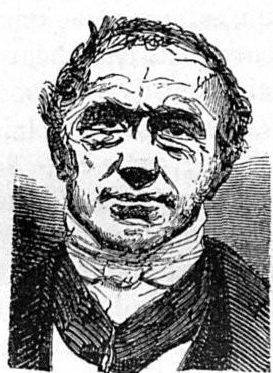
\includegraphics[width=\linewidth]{figures/legendre.png}
%    \captionof*{figure}{\tiny A-M. Legendre}
%  \end{minipage}}%
%  \hfill
%  \begin{minipage}[b]{0.46\textwidth}
%    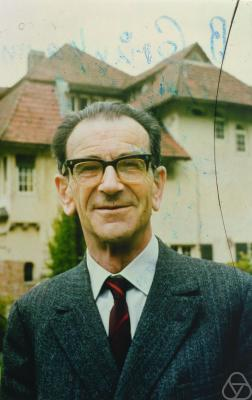
\includegraphics[width=\linewidth]{figures/Werner_Fenchel.jpeg}
%    \captionof*{figure}{\tiny W. Fenchel}
%  \end{minipage}
%\end{figure}
%
%\end{minipage}
%\begin{beamercolorbox}[rounded=true, shadow=true, wd=\textwidth]{block title}\centering
%$f^*$ is convex (prove this), but it may be nowhere finite.
%\end{beamercolorbox}
%\end{frame}

%\begin{frame}[plain,c]
%\centering
%\begin{tikzpicture}
%  \begin{axis}[
%      axis lines=middle,
%      xlabel={$x$},
%      ylabel={$f(x)$},
%      domain=0.1:4,
%      samples=200,
%      ymin=-2.5, ymax=2.5,
%      xmin=0, xmax=4,
%      legend style={at={(0.5,1.0)}, anchor=north},
%      thick
%    ]
%    
%    % Function
%    \addplot[blue, ultra thick, domain=0.1:4] {x*ln(x) - x};
%    \addlegendentry{$f(x) = x \ln x - x$}
%    
%    % Tangents at x0, x1, x2
%    % x0 = 0.5
%    \pgfmathsetmacro\xA{0.5}
%    \pgfmathsetmacro\yA{\xA*ln(\xA) - \xA}
%    \pgfmathsetmacro\mA{ln(\xA)}
%    \addplot[red,  thick, domain=0.1:4] {\mA*(x - \xA) + \yA};
%    \addplot[only marks, mark=*] coordinates {(\xA,\yA)};
%    \node[below left] at (axis cs:\xA,\yA) {$x_0$};
%
%    % x1 = 1.5
%    \pgfmathsetmacro\xB{1.5}
%    \pgfmathsetmacro\yB{\xB*ln(\xB) - \xB}
%    \pgfmathsetmacro\mB{ln(\xB)}
%    \addplot[green!70!black,  thick, domain=0.1:4] {\mB*(x - \xB) + \yB};
%    \addplot[only marks, mark=*] coordinates {(\xB,\yB)};
%    \node[below right] at (axis cs:\xB,\yB) {$x_1$};
%
%    % x2 = 3.0
%    \pgfmathsetmacro\xC{3.0}
%    \pgfmathsetmacro\yC{\xC*ln(\xC) - \xC}
%    \pgfmathsetmacro\mC{ln(\xC)}
%    \addplot[orange!80!black,  thick, domain=0.1:4] {\mC*(x - \xC) + \yC};
%    \addplot[only marks, mark=*] coordinates {(\xC,\yC)};
%    \node[above right] at (axis cs:\xC,\yC) {$x_2$};
%
%  \end{axis}
%\end{tikzpicture}\vspace{2ex}
%\begin{beamercolorbox}[rounded=true, shadow=true, wd=\textwidth]{block title}\small
%The Fenchel conjugate $f^*$ encodes all the information of the convex hull of $f(x)$'s epigraph in terms of its supporting hyperplanes, i.e.
%\[
%f^*(x^*) := \sup_{x \in X} \left\{\langle x^*,x\rangle - f(x) \right\}.
%\]\vspace{-2.5ex}
%\end{beamercolorbox}
%\end{frame}

%\begin{frame}\frametitle{An Example}
%\begin{example}
%Let $f(x) = \exp x$. Then $f: \mathbb R \to \mathbb R$ and $f^* : \mathbb R \to \overline{\mathbb R}$ is given by
%\[
%f^*(x^*) := \sup_{x \in \mathbb R}\{ x^* x - \exp(x) \} = - \inf_{x \in \mathbb R}\{\exp(x) - x^* x\}.
%\]
%\visible<2->{If $x^* < 0$, then $x\to -\infty$ implies $x^* x - \exp(x) \to +\infty$. Hence, $f^*(x^*) = +\infty$. \medskip}
%
%\visible<3->{If $x^* = 0$, then the least upper bound of $-\exp(x)$ over $x \in \mathbb R$ is 0. Hence, $f^*(x^*) = 0$.  \medskip}
%
%\visible<4->{If $x^* > 0$, then the minimizer of $\exp(x) - x^*x$ solves $\exp(x) = x^*$, i.e., $x = \ln(x^*)$. \medskip}
%
%\visible<5->{So the \alert{convex conjugate} of \alert{$f(x) = \exp(x)$} is Shannon's entropy extended to $\mathbb R$.}
%\end{example}
%\end{frame}

%\begin{frame}\frametitle{The Hellinger Entropy}
%\begin{example}
%Let $f(x) = -\sqrt{1 - \|x\|^2}$ with $f(x) = +\infty$ for $\|x\| > 1$. Here, we have for $\|x\| \le 1$
%\[ 
%(\langle x^*, \cdot\rangle - f(\cdot))'(x) = x^* -  (1 - \|x\|^2)^{-1/2} x \Rightarrow x(x^*) = \frac{x^*}{\sqrt{1 + \|x^*\|^2}}
%\]
%By substitution, we get
%\[
%f^*(x^*) = \frac{1 + \|x^*\|^2}{\sqrt{1 + \|x^*\|^2}}.
%\]
%Note: 
%\[
%\nabla f^*(x^*) = \frac{x^*}{\sqrt{1 + \|x^*\|^2}} \text{ and } \| \nabla f^*(x^*) \| \le 1.
%\]
%\end{example}
%\end{frame}

\begin{frame}\frametitle{Observation}
\begin{beamercolorbox}[rounded=true, shadow=true, wd=\textwidth]{block body}
Given\footnote{\tiny $R_1$ is known as Shannon's entropy and $R_2$ is Hellinger's entropy.} $R_1(a) := a \ln a - a$ and $R_2(a) := -\sqrt{1 - \|a\|^2}$ we see that 
\[
R_1^*(a^*) = \exp(a^*) \text{ and } R^*_2(a^*) = \frac{1 + \|a^*\|^2}{\sqrt{1 + \|a^*\|^2}}.
\]\visible<2->{
Moreover, though $R_1$, $R_2$ have restricted domains, $R^*_1$, $R^*_2$ are defined on all of $\mathbb R^n$.\medskip}

\visible<3->{What's more: $\nabla R^*_1(a^*) = \exp(a^*)$ and $\nabla R^*_2(a^*) =  \frac{a^*}{\sqrt{1 + \|a^*\|^2}}$}\visible<3->{ and 
\[
\nabla R^*_1(\mathbb R) \subset \mathrm{int \, dom\,} R_1 \text{ and } \nabla R^*_2(\mathbb R^n) \subset \mathrm{int \, dom\,} R_2.
\]}\vspace{-2ex}
\end{beamercolorbox}

\visible<4->{
\begin{beamercolorbox}[rounded=true, shadow=true, wd=\textwidth]{block body}\centering
Is there are general class of functions $R$ for which $\nabla R^*$ maps into  $\mathrm{int \, dom\,} R$? \alert{Yes!}.
\end{beamercolorbox}}
\end{frame}

\begin{frame}\frametitle{Legendre Functions\footnote{\tiny Originally introduced by Rockafellar in 1967, we follow the definition and nomenclature of Teboulle (2018)}}

%\visible<1->{
%\begin{beamercolorbox}[rounded=true, shadow=true, wd=\textwidth]{block body}\centering
%The geometry of a closed convex set $C \subset \mathbb{R}^m$ with a non-empty interior, $\operatorname{int}C \neq \emptyset$, can be encoded into a \alert{Legendre function} $R: \mathbb{R}^m \to \mathbb{R}\cup\{+\infty\}$.
%\end{beamercolorbox}}

\begin{minipage}{0.7\textwidth}
\begin{definition}[]
%\label{def:LegendreFunction}
\visible<2->{
Let the essential domain of a function $R$ be defined as $\operatorname{dom} R := \{ a \in \mathbb{R}^m \mid R(a) < \infty \}$.
}\visible<3->{We call a proper convex function a \alert{Legendre function} $R: \mathbb{R}^m \to \mathbb{R}\cup\{+\infty\}$ if}
\begin{itemize}
%% \itemsep=-3pt
\item \visible<4->{$\operatorname{int}(\operatorname{dom} R) \neq \varnothing$;}
\item \visible<5->{$R$ is differentiable on $\operatorname{int}(\operatorname{dom} R)$;}
\item \visible<6->{$\lim_{t \to 0^+} \langle \nabla R(a+t(b-a)), b-a\rangle = -\infty$ for all $a \in \partial( \operatorname{dom} R)$ and $b \in \operatorname{int}(\operatorname{dom} R)$;}
\item \visible<7->{R is strictly convex on $\operatorname{int}(\operatorname{dom} R)$.}
\end{itemize}
\end{definition}
\end{minipage}\hfill
\begin{minipage}{0.3\linewidth}
 \centering
 \begin{figure}
  \centering\vspace{1ex}
  \begin{minipage}[b]{0.6\textwidth}
    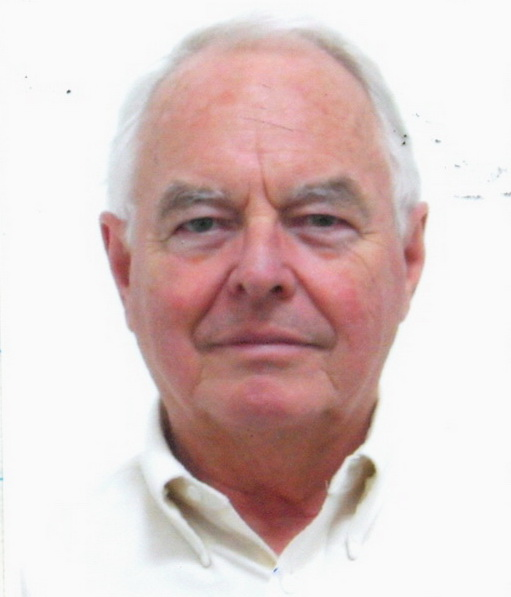
\includegraphics[width=\linewidth]{figures/rtr.jpg}
    \captionof*{figure}{\tiny R. Tyrrell Rockafellar}
  \end{minipage}%
  \end{figure}
  \end{minipage}



%Introduced by Rockafellar in 1967~\cite{Rockafellar1967Conjugates}, see also \cite[Chap.~26]{RTRockafellar_1970}, Legendre functions constitute a special class of proper convex functions whose gradients $\nabla R$ become singular on the boundary of their essential domains.
%We denote by $R^*(a^\ast) \coloneqq \sup \{ a \cdot a^\ast - R(a) \mid a \in \mathbb{R}^m \}$ the convex conjugate of $R$.
%
%\begin{theorem}[Rockafellar \text{\cite[Thm. 1]{Rockafellar1967Conjugates}}]
%\label{thm:Rockafellar}
%A proper convex function $R$ is a Legendre function if and only if its convex conjugate $R^\ast$ is also a Legendre function.
%Moreover, $\nabla R \colon \operatorname{int}(\operatorname{dom} R) \to \operatorname{int}(\operatorname{dom} R^*)$ is a topological isomorphism with $(\nabla R)^{-1} = \nabla R^\ast$.
%\end{theorem}
%
%
%From now on, we assume that ${R(a)}/{|a|} \to +\infty$ as $|a| \to \infty$ and $\operatorname{dom} R = C$.
\end{frame}

\begin{frame}\frametitle{Properties of Legendre Functions}

\visible<1->{
\begin{beamercolorbox}[rounded=true, shadow=true, wd=\textwidth]{block body}\centering
 Legendre functions constitute a special class of proper convex functions whose gradients $\nabla R$ become singular on the boundary of their essential domains.
\end{beamercolorbox}}

\begin{minipage}{0.7\textwidth}
\begin{theorem}[Rockafellar (1967)]
\label{thm:Rockafellar}
A proper convex function $R$ is a Legendre function if and only if its convex conjugate $R^\ast$ is also a Legendre function.
Moreover, $\nabla R \colon \operatorname{int}(\operatorname{dom} R) \to \operatorname{int}(\operatorname{dom} R^*)$ is a topological isomorphism with $(\nabla R)^{-1} = \nabla R^\ast$.
\end{theorem}
\end{minipage}\hfill
\begin{minipage}{0.3\linewidth}
 \centering
 \begin{figure}
  \centering\vspace{1ex}
  \begin{minipage}[b]{0.6\textwidth}
    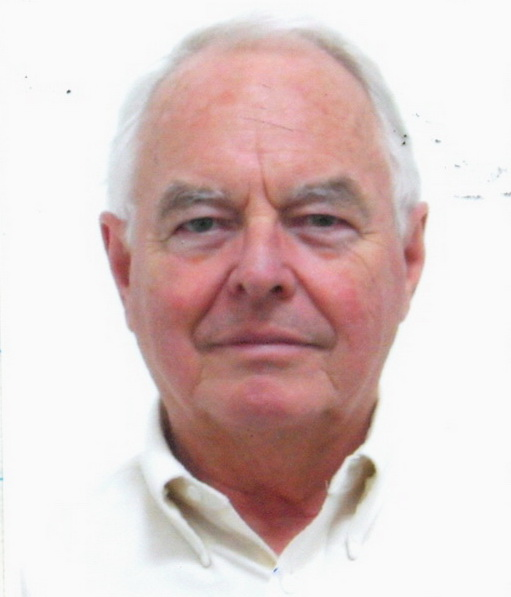
\includegraphics[width=\linewidth]{figures/rtr.jpg}
    \captionof*{figure}{\tiny R. Tyrrell Rockafellar}
  \end{minipage}%
  \end{figure}
  \end{minipage}

\visible<2->{
\begin{beamercolorbox}[rounded=true, shadow=true, wd=\textwidth]{block title}\centering
It can also be shown that ${R(a)}/{|a|} \to +\infty$ as $|a| \to \infty$ if and only if $\operatorname{dom} R^* = \mathbb R^n$.
\end{beamercolorbox}}

\end{frame}

\begin{frame}\frametitle{Geometry Preserving Transformations}

\begin{beamercolorbox}[rounded=true, shadow=true, wd=\textwidth]{block title}
\begin{equation*} \label{eq:intro:feasible_set}
K = \{ v \in V \mid Bv(x) \in C(x) \text{ for almost every } x \in \Omega_d \subset \overline{\Omega} \}.
\end{equation*}
\end{beamercolorbox}\hfill

\begin{minipage}{0.5\linewidth}
\begin{beamercolorbox}[rounded=true, shadow=true, wd=\textwidth]{block title}
\centering
 $\nabla R \colon \operatorname{int}C \to \operatorname{int}(\operatorname{dom} R^*)$ satisfies %is a topological isomorphism 
 $(\nabla R)^{-1} = \nabla R^\ast$
\end{beamercolorbox}
\end{minipage}
%
\begin{minipage}{0.4\linewidth}
\begin{figure}[h]
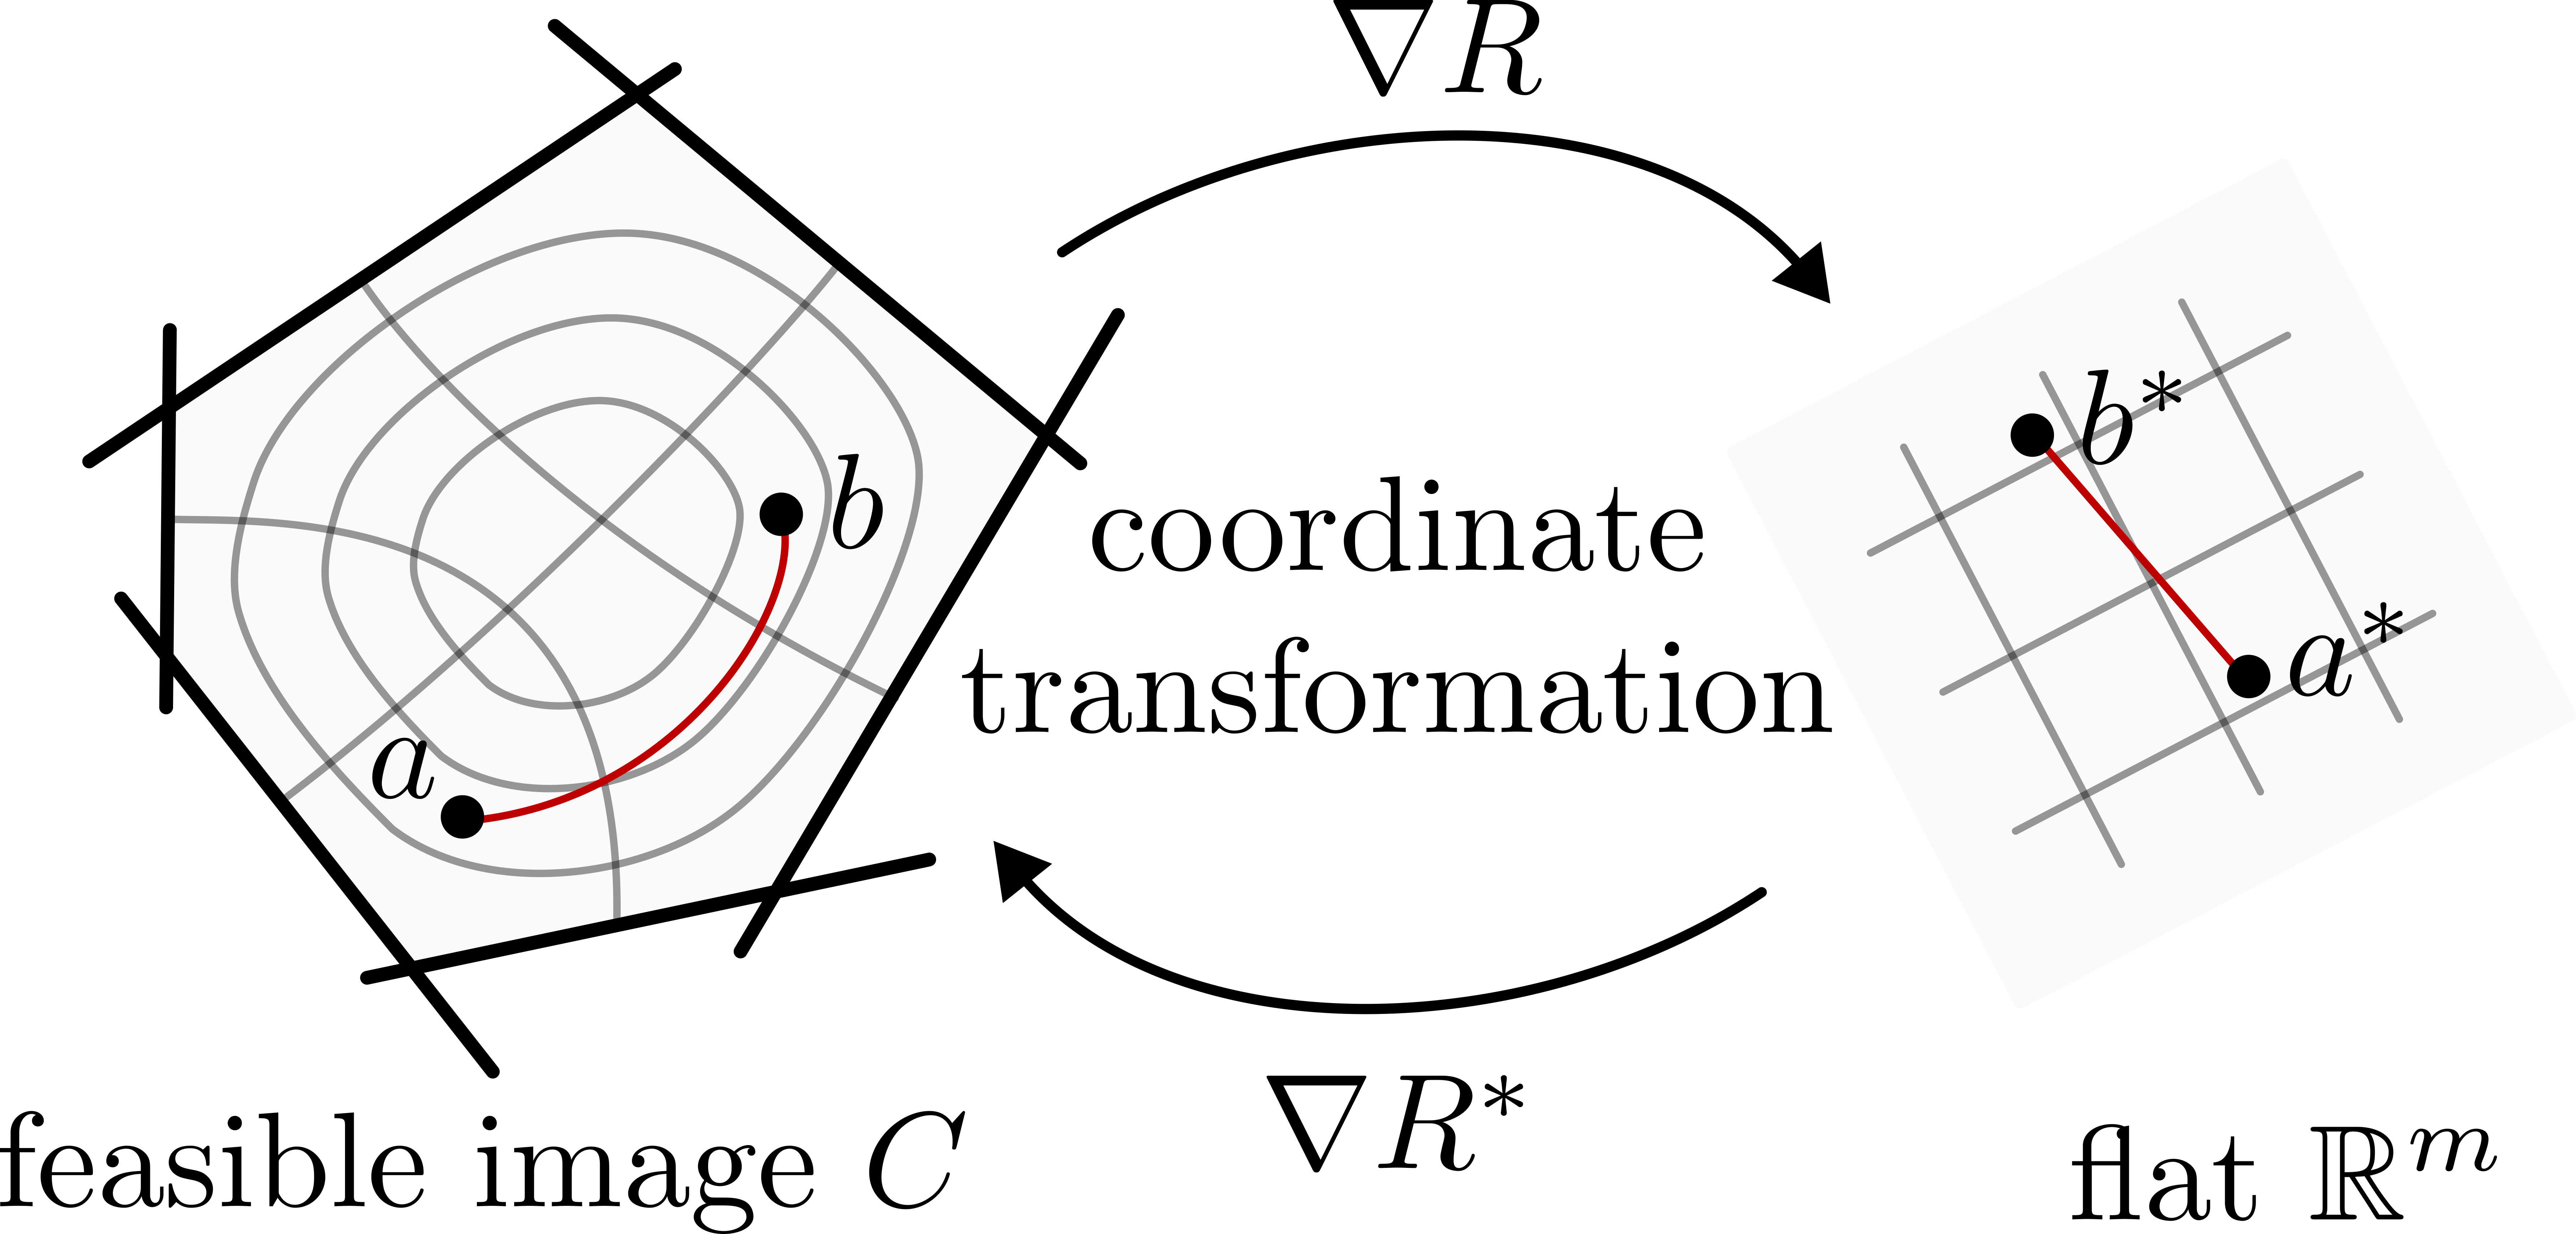
\includegraphics[width=0.8\linewidth]{figures/Geodesic3.png} 
\end{figure}
\end{minipage}
\end{frame}

\subsection{The General LVPP Algorithm}

\begin{frame}[plain,c]
%\frametitle{A first slide}
\hfill
\begin{center}
\Large With the help of Legendre functions, we can find mappings that \alert{guarantee} feasibility for pointwise inequality constraints.
\end{center}
\hfill
\end{frame}

\begin{frame}\frametitle{}
\thispagestyle{empty}
%\hypertarget{lvpp-table}{}
%\hyperlink{lvpp-examples}{\beamerbutton{Go to Examples}}
\begin{table}
\centering
\small
% \renewcommand{\arraystretch}{0.6}
\setlength{\tabcolsep}{5pt}
\renewcommand{\arraystretch}{1.4}
    \begin{tabular}{ c|c|c|c } 
     \toprule
      Feasible set $K$ & Legendre function $R$ & $B$ & $\nabla R^*(\psi)$ \\ 
     \midrule
     $\big\{ u \geq \phi \big\}$ & $(a - \phi) \ln (a - \phi) - (a - \phi)$ & $\operatorname{id}$ & $\phi + \exp\psi$ \\[2ex]
     $\big\{ \phi_1 \leq u \leq \phi_2 \big\}$ & $(a - \phi_1) \ln (a - \phi_1) + (\phi_2-a) \ln (\phi_2-a)$ & $\operatorname{id}$ & $\dfrac{\phi_1 + \phi_2\exp\psi}{1 + \exp\psi}$ \\[2ex]
     % $\big\{ \phi_1 \leq u \leq \phi_2 \big\}$ & $\sum_{i=1}^2 (-1)^i (\phi_i - a) \ln \left( (-1)^i (\phi_i - a)\right)$ & $\operatorname{id}$ & $\dfrac{\phi_1 + \phi_2\exp\psi}{1 + \exp\psi}$ \\[2ex]
     $\big\{\gamma u \ge \phi \big\}$ & $(a-\phi) \ln (a - \phi) - (a - \phi)$ & $\gamma$ &  $\phi + \exp\psi$ \\[2ex]
     $\big\{ (\gamma u)\cdot n \leq \phi \big\}$ & $(\phi-a) \ln (\phi - a) - (\phi - a)$ & $\gamma(\cdot) \cdot n$ & $\phi - \exp(-\psi)$ \\[2ex]
     $\big\{| \nabla u | \le \phi \big\}$ & $ -\sqrt{\phi^2 - | a |^2}$ & $\nabla$  & $\dfrac{\phi\psi}{\sqrt{1 + | \psi |^2}}$ \\[3ex] 
     $\big\{ u \ge 0,\; \sum_{i} u_i = 1 \big\}$ & $\sum_{i} a_i \ln(a_i)$ & $\operatorname{id}$ & $\dfrac{\exp\psi}{\sum_{i} \exp\psi_i}$\\[2ex]
     $\big\{ \det (\nabla^2 u) \geq 0 \big\}$ & $\operatorname{tr}(a\ln a - a)$ & $\nabla^2$ & $\exp \psi$ \\[2ex]
     \bottomrule
    \end{tabular}
\vspace{-1em}
%\end{sidewaystable}
\end{table}
\end{frame}

\begin{frame}\frametitle{The LVPP Algorithm}
\begin{beamercolorbox}[rounded=true, shadow=true, wd=\textwidth]{block body}
Taking $\mathop{\text{dom}}R(\cdot,x) := C(x)$ brings us back to proximal point:\medskip

\visible<2->{Given $u^0 \in V$ and $\left\{\alpha_k\right\}$ find $u \in \mathop{\text{argmin}}_{v \in K} J(v)$  by recursively computing} 
\visible<3->{
\begin{equation}\label{eq:lvpp-op}
\only<3>{
u^{k} \in \mathop{\text{argmin}}_{u \in K} J(u) + \alpha_{k}^{-1} \int_{\Omega_d} D_R(Bu, Bu^{k-1}) \dd \mathcal{H}_d, \quad k = 1, 2, \dots.
}
\only<4->{
    \text{Find } u^k \in K: \quad \underbrace{\alpha_k J^\prime(u^k) +  B^* \nabla R(Bu^k) - B^* \nabla R(Bu^{k-1}) = 0,}_{\text{Properties of $R$ force constraints to be inactive for $u^k$} }
}
\end{equation}\vspace{-2ex}
}\end{beamercolorbox}
\visible<5->{
\begin{beamercolorbox}[rounded=true, shadow=true, wd=\textwidth]{block body}
Using again \alert{latent variables}: given $\psi^0 \in W$, find $(u^{k}, \psi^{k}) \in V \times W$ satisfying
\begin{subequations} \label{eq:intro:lvpp}
\begin{align}
\label{eq:intro:lvpp:a}
\alpha_{k} J'(u^{k}) + B^*\psi^{k} &= B^*\psi^{k-1}, \\
\label{eq:intro:lvpp:b}
Bu^{k} - \nabla R^*(\psi^{k}) &= 0
\end{align}
\end{subequations}\vspace{-4ex}
\end{beamercolorbox}\centering
}
%\visible<6->{
%\begin{minipage}{0.4\linewidth} 
%\begin{beamercolorbox}[rounded=true, shadow=true, wd=\textwidth]{block title}
%\centering
%\textbf{\eqref{eq:intro:lvpp:b} implies }$Bu^k \in  \nabla R^*(W) \subset C$!\\
%Clearly, $\nabla R^*(W_h) \subset C$, as well.
%\end{beamercolorbox}
%\end{minipage}
%}
%\visible<7->{ 
%\begin{minipage}{0.5\linewidth} 
%\begin{beamercolorbox}[rounded=true, shadow=true, wd=\textwidth]{block title}
%\centering
%A new, unifying perspective on pointwise inequality constraints.
%\end{beamercolorbox}
%\end{minipage}
%}
\end{frame}

%\begin{frame}\frametitle{A}
%\begin{itemize}
%\item Define proper, convex, lsc again
%\item Define convex conjugate and motivate its meaning
%\item Define Legendre function
%\item Find a picture of Rockafellar
%\item Work out two examples to show how to compute the convex conjugate
%\item Prove (if possible) the crucial Rockafellar theorems
%\item Give the table in the paper
%\item Return to Bregman 
%\end{itemize}
%\end{frame}





\subsection{Applications}

%\begin{frame}\frametitle{The Signorini Problem}
%\begin{minipage}{0.55\linewidth}
%\visible<1->{
%\begin{beamercolorbox}[rounded=true, shadow=true, wd=\textwidth]{block body}
%Signorini (1959), analyzed by Fichera (1963).\\
% 
%The essential first problem in contact mechanics.\\
% 
%Models the deformation of a linear elastic body in the presence of a contact boundary constraint.
%\end{beamercolorbox}
%}\visible<2->{
%\begin{beamercolorbox}[rounded=true, shadow=true, wd=\textwidth]{block body}
%\visible<2->{$\Omega \subset \mathbb{R}^3$, $\Gamma$ split into two disjoint subsets.}
%\visible<2->{$\Gamma = \overline{ \Gamma_\mathrm{D} \cup \Gamma_\mathrm{T} }$ with\\
%$\Gamma_D$ for \textbf{d}isplacement\\
%$\Gamma_{T}$ for \textbf{t}raction boundary conditions.}
%\end{beamercolorbox}}
%\end{minipage}\hspace{4ex}
%\begin{minipage}{0.3\linewidth}
% \centering
% \begin{figure}
%  \centering\vspace{1ex}
%  \visible<1->{\begin{minipage}[b]{0.45\textwidth}
%    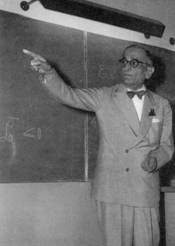
\includegraphics[width=\linewidth]{figures/Antonio_Signorini.jpg}
%    \captionof*{figure}{\tiny A. Signorini}
%  \end{minipage}}%
%  \hfill
%  \begin{minipage}[b]{0.46\textwidth}
%    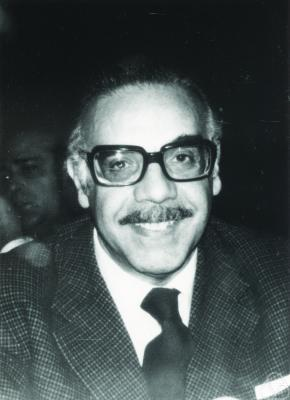
\includegraphics[width=\linewidth]{figures/Gaetano_Fichera.jpg}
%    \captionof*{figure}{\tiny G. Fichera}
%  \end{minipage}
%\end{figure}\vspace{-8ex}
%\begin{figure}
%	\centering
%	\begin{tikzpicture}
%		\node at (-3.35,0) {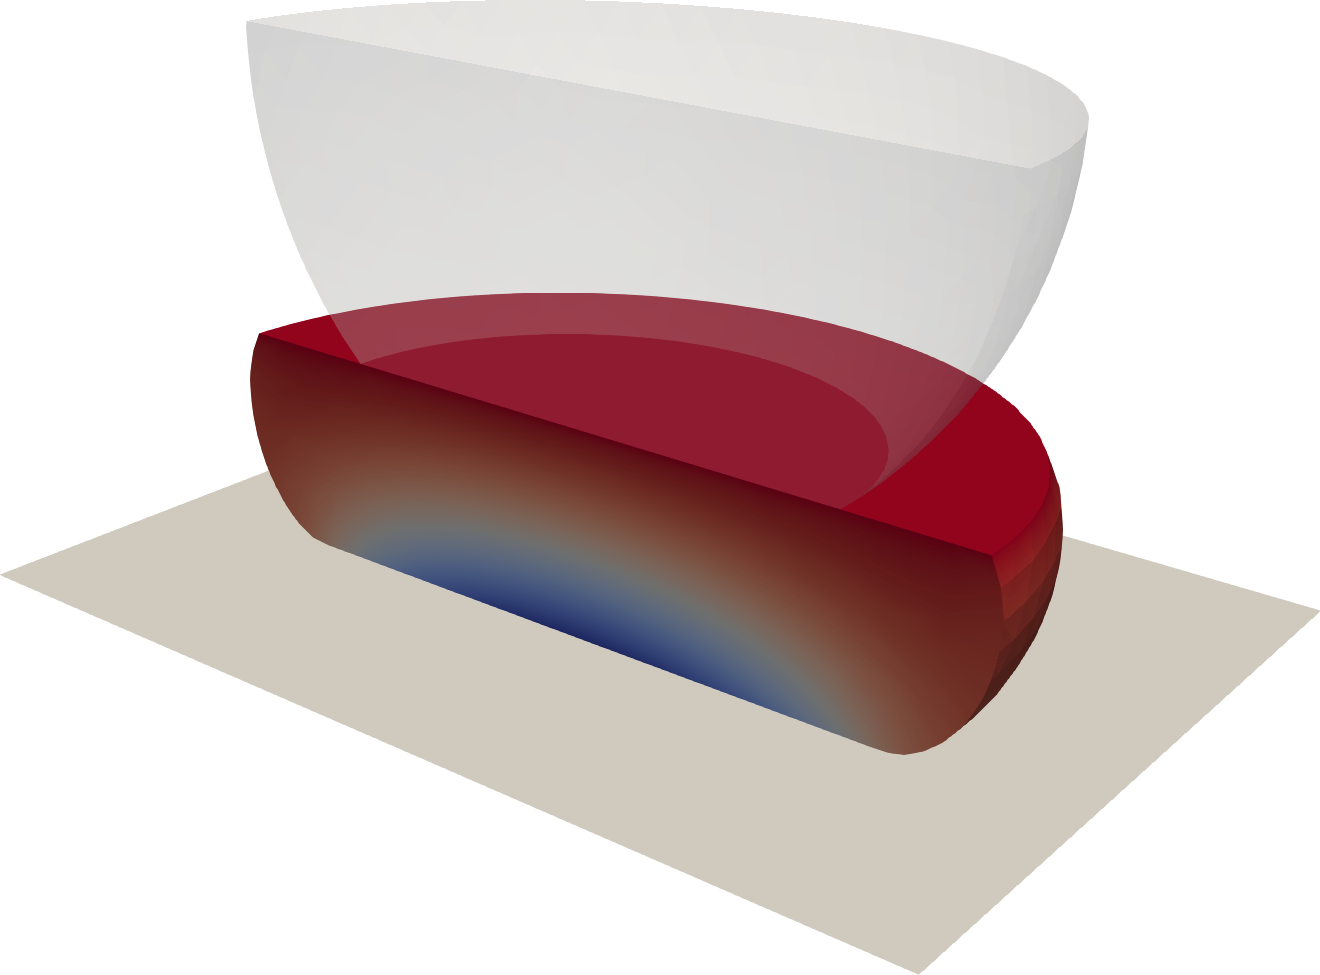
\includegraphics[height=1.25in]{figures/contact.png}};
%    \end{tikzpicture}
%\end{figure}
%\end{minipage}
%\end{frame}

%\begin{frame}\frametitle{The Signorini Problem}
%\begin{minipage}{0.55\linewidth}
%\visible<1->{
%\begin{beamercolorbox}[rounded=true, shadow=true, wd=\textwidth]{block body}
%\visible<1->{State space:\vspace{-1.5ex}
%\begin{equation*}
%\label{eq:Signorini_V}
%    V = \big\{ u \in H^1(\Omega,\mathbb{R}^3)
%        \mid u = g \text{ on } \Gamma_\mathrm{D\textbf{}}
%    \big\}
%    \,,
%\end{equation*}}\vspace{-4ex}
%
%\visible<2->{Objective function:\vspace{-1.5ex}
%\begin{equation*}
%    J(u) =
%    \frac{1}{2}\int_\Omega (\mathbb C \epsilon(u)) : \epsilon(u) \dd x
%    -
%    \int_\Omega f \cdot u \dd x
%    \,,
%\end{equation*}}\vspace{-2.5ex}
%
%\visible<3->{Inequality constraints:\vspace{-1ex}
%\begin{equation*}
% \alert{   K = \big\{ u \in V
%        \mid u \cdot \tilde{n} \leq \phi_1 \text{ on } \Gamma_\mathrm{T}
%    \big\} }
%    \,.
%\end{equation*}}\vspace{-4ex}
%\end{beamercolorbox}
%}\visible<4->{
%\begin{beamercolorbox}[rounded=true, shadow=true, wd=\textwidth]{block body}\scriptsize
%%Here, $\epsilon : H^1(\Omega,\mathbb{R}^3) \to L^2(\Omega,\mathbb{R}^{3\times 3}_{\mathrm{sym}})$, 
%$\epsilon := (\nabla + \nabla^\top)/2$ symmetric gradient\smallskip
% 
%$\C \colon \mathbb{R}^{3\times 3}_{\mathrm{sym}} \to \mathbb{R}^{3\times3}_{\mathrm{sym}}$ sym.\ pos.-def.\ elasticity tensor\smallskip
%
%$f \colon \Omega \to \mathbb{R}^3$ internal body force density\smallskip
%
%$\phi_1 \colon \Gamma_\mathrm{T} \to \mathbb{R}_+$ gap function, $\tilde{n}$ normal to contact surface.
%\end{beamercolorbox}}
%\end{minipage}\hspace{4ex}
%\begin{minipage}{0.3\linewidth}
% \centering
% \begin{figure}
%  \centering\vspace{1ex}
%  \visible<1->{\begin{minipage}[b]{0.45\textwidth}
%    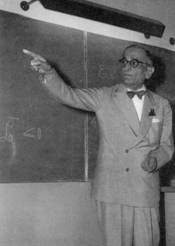
\includegraphics[width=\linewidth]{figures/Antonio_Signorini.jpg}
%    \captionof*{figure}{\tiny A. Signorini}
%  \end{minipage}}%
%  \hfill
%  \begin{minipage}[b]{0.46\textwidth}
%    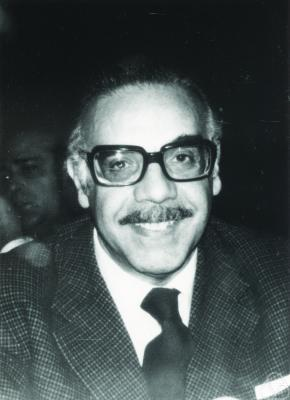
\includegraphics[width=\linewidth]{figures/Gaetano_Fichera.jpg}
%    \captionof*{figure}{\tiny G. Fichera}
%  \end{minipage}
%\end{figure}\vspace{-8ex}
%\begin{figure}
%	\centering
%	\begin{tikzpicture}
%		\node at (-3.35,0) {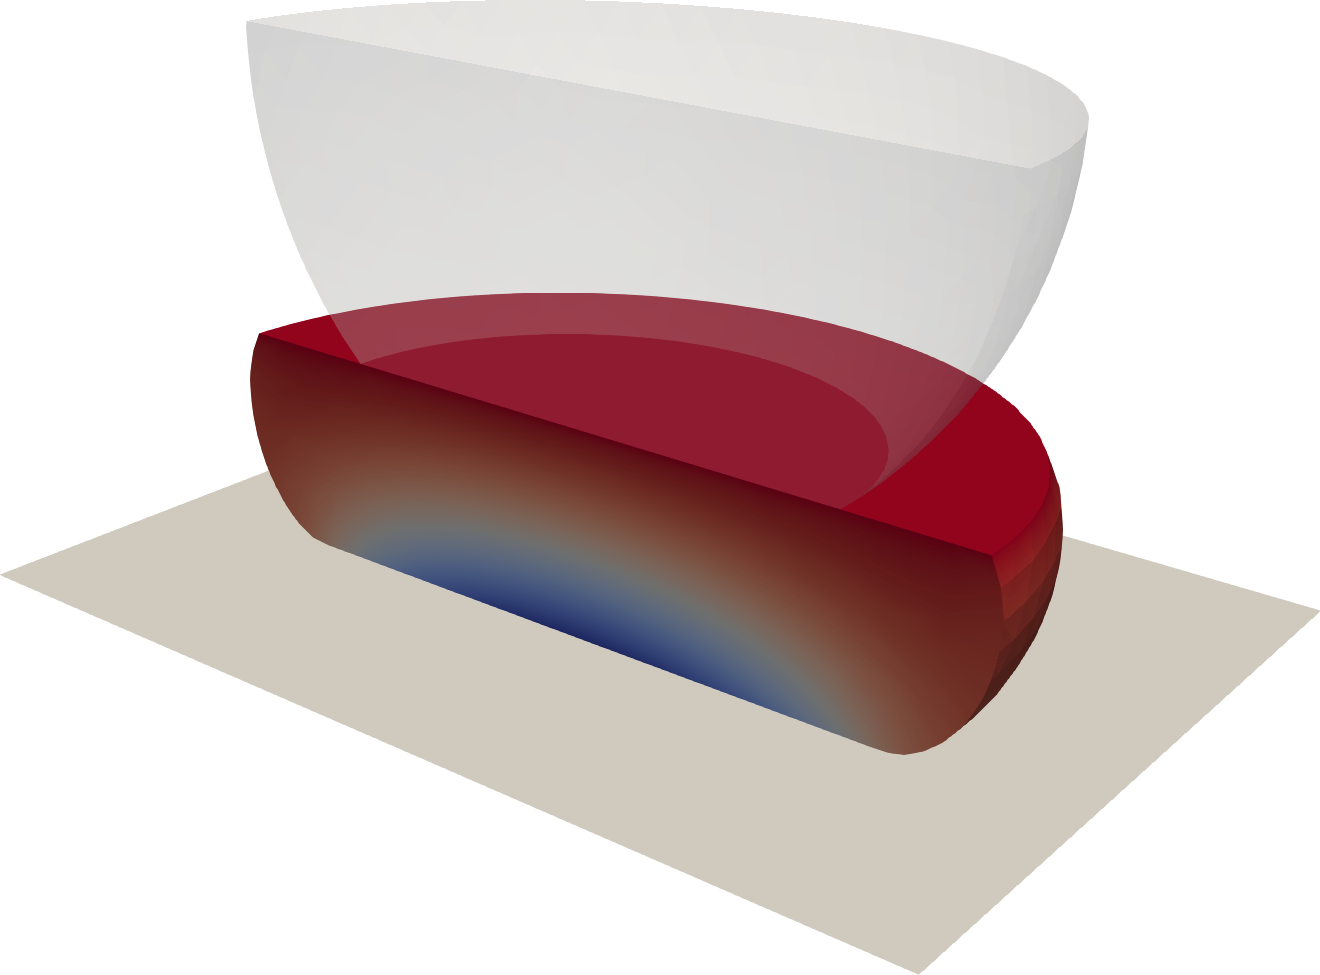
\includegraphics[height=1.25in]{figures/contact.png}};
%    \end{tikzpicture}
%\end{figure}
%\end{minipage}
%\end{frame}

\begin{frame}\frametitle{LVPP for Signorini}
\begin{minipage}{\linewidth}
\begin{beamercolorbox}[rounded=true, shadow=true, wd=\textwidth]{block body}

\begin{columns}
\begin{column}{0.55\textwidth}
\begin{itemize}
\item $B := \gamma(\cdot) \cdot \tilde{n}$ (trace on contact boundary)
\item $\Omega_d := \Gamma_\mathrm{T}$
\item $C(x) := (-\infty,\phi_1(x)]$
\item $R(a) := (a-\phi) \ln (a - \phi) - (a - \phi)$
\item $\psi^0 = 0$
\end{itemize}
\end{column}
\begin{column}{0.3\textwidth}  %%<--- here
\begin{minipage}{0.3\linewidth}
 \centering
\begin{figure}
	\centering
	\begin{tikzpicture}
		\node at (-7.35,0) {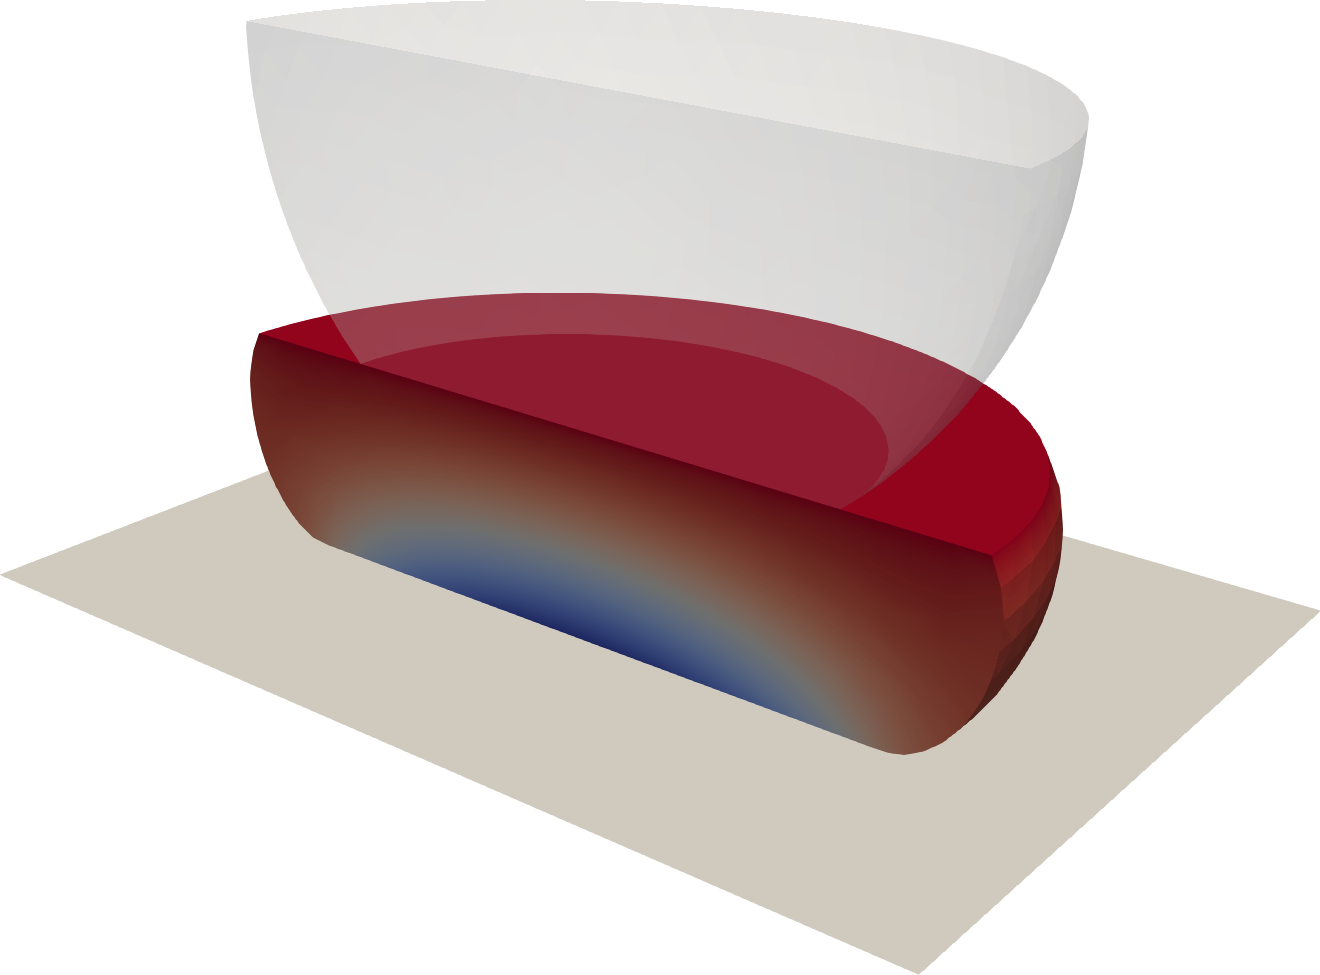
\includegraphics[height=1.25in]{figures/contact.png}};
    \end{tikzpicture}
\end{figure}
\end{minipage}
\end{column}
\end{columns}\visible<2->{
%The LVPP saddle-point problems:\\
Find $(u^{k}, \psi^{k}) \in V \times L^\infty(\Gamma_\mathrm{T})$ satisfying
\begin{subequations}
\label{eq:SignoriniVF}
\begin{align}
    ( \alpha_k\C \epsilon(u^k), \epsilon(v) ) - (\psi^k, v\cdot \tilde{n} )_{\Gamma_\mathrm{T}}
    &=
    (\alpha_k f, v) - ( \psi^{k-1}, v \cdot \tilde{n} )_{\Gamma_\mathrm{T}}
    \,,
    \\
    ( u^k\cdot \tilde{n} , w )_{\Gamma_\mathrm{T}} + ( \exp \psi^k, w )_{\Gamma_\mathrm{T}}
    &= ( \phi_1, w )_{\Gamma_\mathrm{T}}
    \,,
\end{align}
\end{subequations}
for all $(v, w) \in V \times L^\infty(\Gamma_\mathrm{T})$, where $(\cdot, \cdot  )_{\Gamma_\mathrm{T}}$ denotes the $L^2(\Gamma_\mathrm{T})$-inner product.}
\end{beamercolorbox}
\end{minipage}
\end{frame}

%\begin{frame}\frametitle{LVPP for Signorini}
%\begin{beamercolorbox}[rounded=true, shadow=true, wd=\textwidth]{block body}
%\begin{itemize}
%%\item Code available here: 
%\item Define a \alert{proximal Galerkin method} using equal-order continuous Lagrange spaces for the displacement $u$ and latent variable $\psi$.
%\item \visible<2->{Note that the spaces are on manifolds of differing dimensions. Hence, the two discrete subspaces are not the same.}
%\item \visible<3->{We used the mixed-dimensional assembly routines in DOLFINx.}
%%\item \visible<4->{The discrete problem is solved for half of a sphere centered at $(0,0,0.5)$ with radius $0.4$ coming into contact with the rigid $x,y$-plane.} 
%%\item \visible<5->{$\tilde{n}=(0,0,-1)^\top$ and $\phi_1$ measures the vertical distance between the $x,y$-plane and the boundary of the half sphere, i.e., $\phi_1(x,y,z) = z$.}
%%\item \visible<6->{Second-order Lagrange elements approximate the geometry, the displacement, and the latent variable.}
%%\item The initial proximity parameter $\alpha_0 = 0.005$ is doubled at each subsequent proximal step (i.e., LVPP iteration). 
%%\item  The tolerance for Newton’s method is set to $10^{-6}$. 
%%\item  The LVPP algorithm requires a total of 13 proximal iterations, amounting to 17 linear solves. The maximum number of Newton steps was 5, the minimum 1. The number of degrees of freedom was $17,613$ for a mesh with $3,661$ cells.
%\end{itemize}
%\end{beamercolorbox}
%\end{frame}

\begin{frame}\frametitle{LVPP for Signorini}
\begin{minipage}{0.55\linewidth}
\begin{beamercolorbox}[rounded=true, shadow=true, wd=\textwidth]{block body}
 \visible<1->{Initial shape: hemisphere centered at $(0,0,0.5)$ with radius $0.4$ coming in contact with $xy$-plane.} \smallskip
 
 \visible<1->{$\tilde{n}=(0,0,-1)^\top$ and $\phi_1(x,y,z) = z$.}\smallskip
 
\visible<1->{Second-order Lagrange elements for geometry, displacement, and the latent variable.}
\end{beamercolorbox}
\visible<2->{
\begin{beamercolorbox}[rounded=true, shadow=true, wd=\textwidth]{block title}
Performance of LVPP:\\
Proximal iterations 13 ($\alpha$ updates)\\
\textbf{Total linear solves: 17}\\
Max Newton steps: 5\\
Min Newton steps: 1
DoFs: 17,613\\
Cells: 3,661
\end{beamercolorbox}}
\end{minipage}\hspace{4ex}
\begin{minipage}{0.3\linewidth}
 \centering
\begin{beamercolorbox}[rounded=true, shadow=true, wd=\textwidth]{block body}
Parameters:\\
$\alpha_0 = 5$E-3\\
$\alpha_{k+1} := 2\alpha_k$\\
${\tt tol_{rel}} = {\tt tol_{abs}}$ = 1E-6
\end{beamercolorbox}
\begin{figure}
	\centering
	\begin{tikzpicture}
		\node at (-3.35,0) {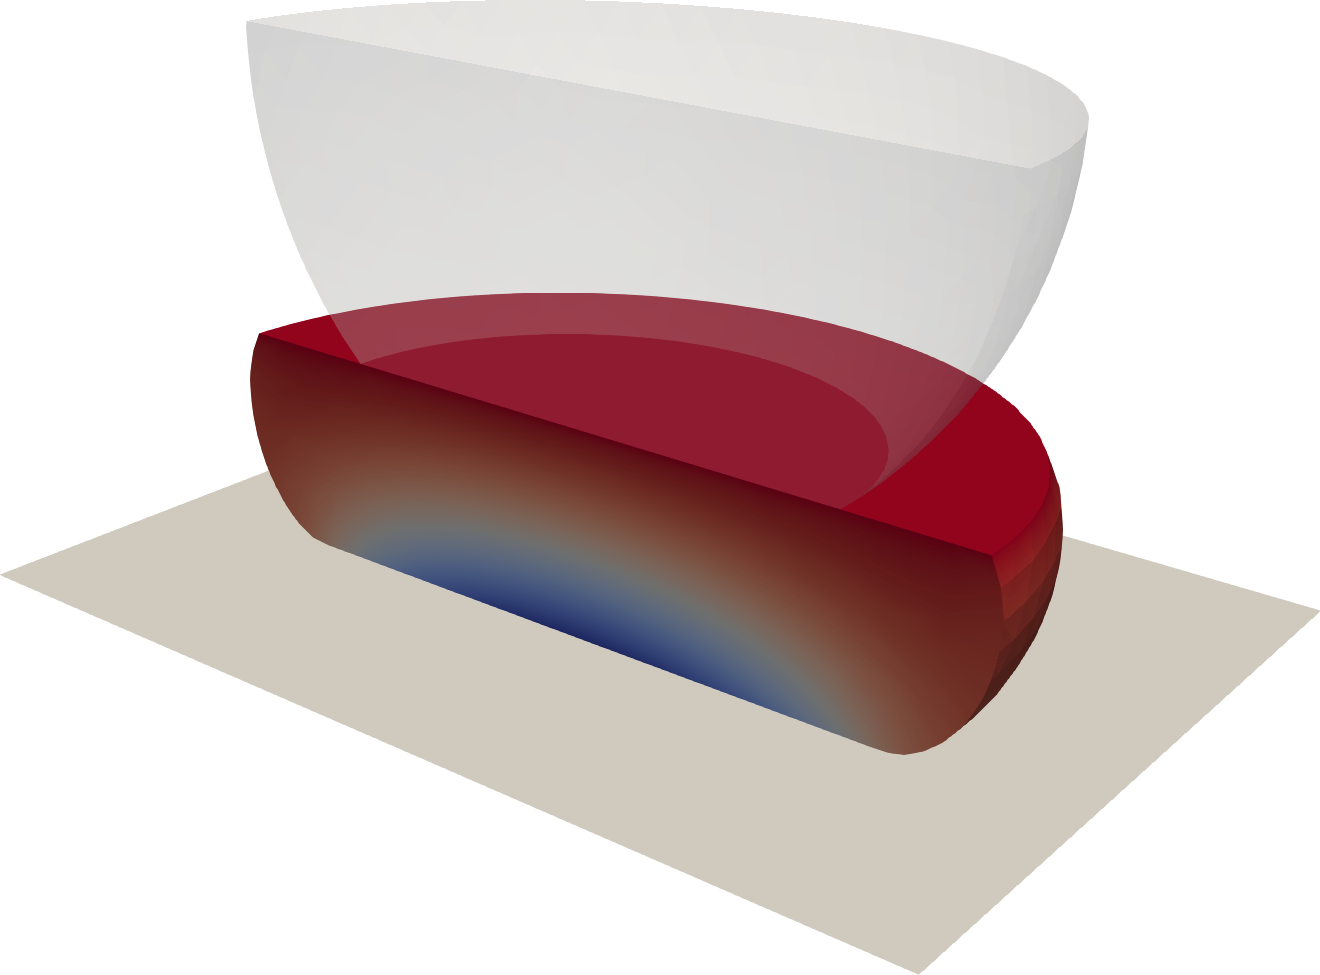
\includegraphics[height=1.25in]{figures/contact.png}};
    \end{tikzpicture}
\end{figure}
\end{minipage}
\end{frame}

\begin{frame}\frametitle{Fully Nonlinear PDEs}
\begin{minipage}{0.5\linewidth}
\begin{beamercolorbox}[rounded=true, shadow=true, wd=\textwidth]{block body}
Many nonlinear  
PDEs have the form:\\ Find $u: \Omega \to \mathbb R$ such that
\begin{equation*}\label{eq:nonlinear-pde}
F(x,u,\nabla u) = 0 \text{ in } \Omega
\text{ and } u = g \text{ on }\partial \Omega\,.
\end{equation*}

This equation lack a divergence structure.\medskip

Integrating by parts will not lead us to the correct notion of a weak solution.%\medskip
%We need the concept of viscosity solution introduced by Crandall and Lions (1983).
\end{beamercolorbox}\hfill\visible<2->{
\begin{beamercolorbox}[rounded=true, shadow=true, wd=\textwidth]{block title}
We need the concept of viscosity solution introduced by Crandall and Lions (1983).
\end{beamercolorbox}}
\end{minipage}\hspace{3ex}
\begin{minipage}{0.35\linewidth}
 \centering
 \begin{figure}
  \centering\vspace{1ex}
  \visible<1->{\begin{minipage}[b]{0.5\textwidth}
    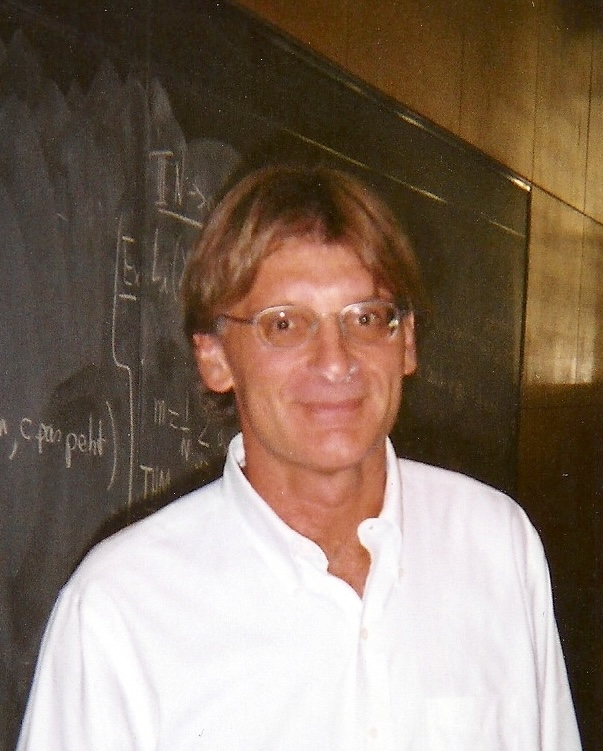
\includegraphics[width=\linewidth]{figures/pllions.jpg}
    \captionof*{figure}{\tiny P.-L. Lions}
  \end{minipage}}%
  \hfill
  \begin{minipage}[b]{0.44\textwidth}
    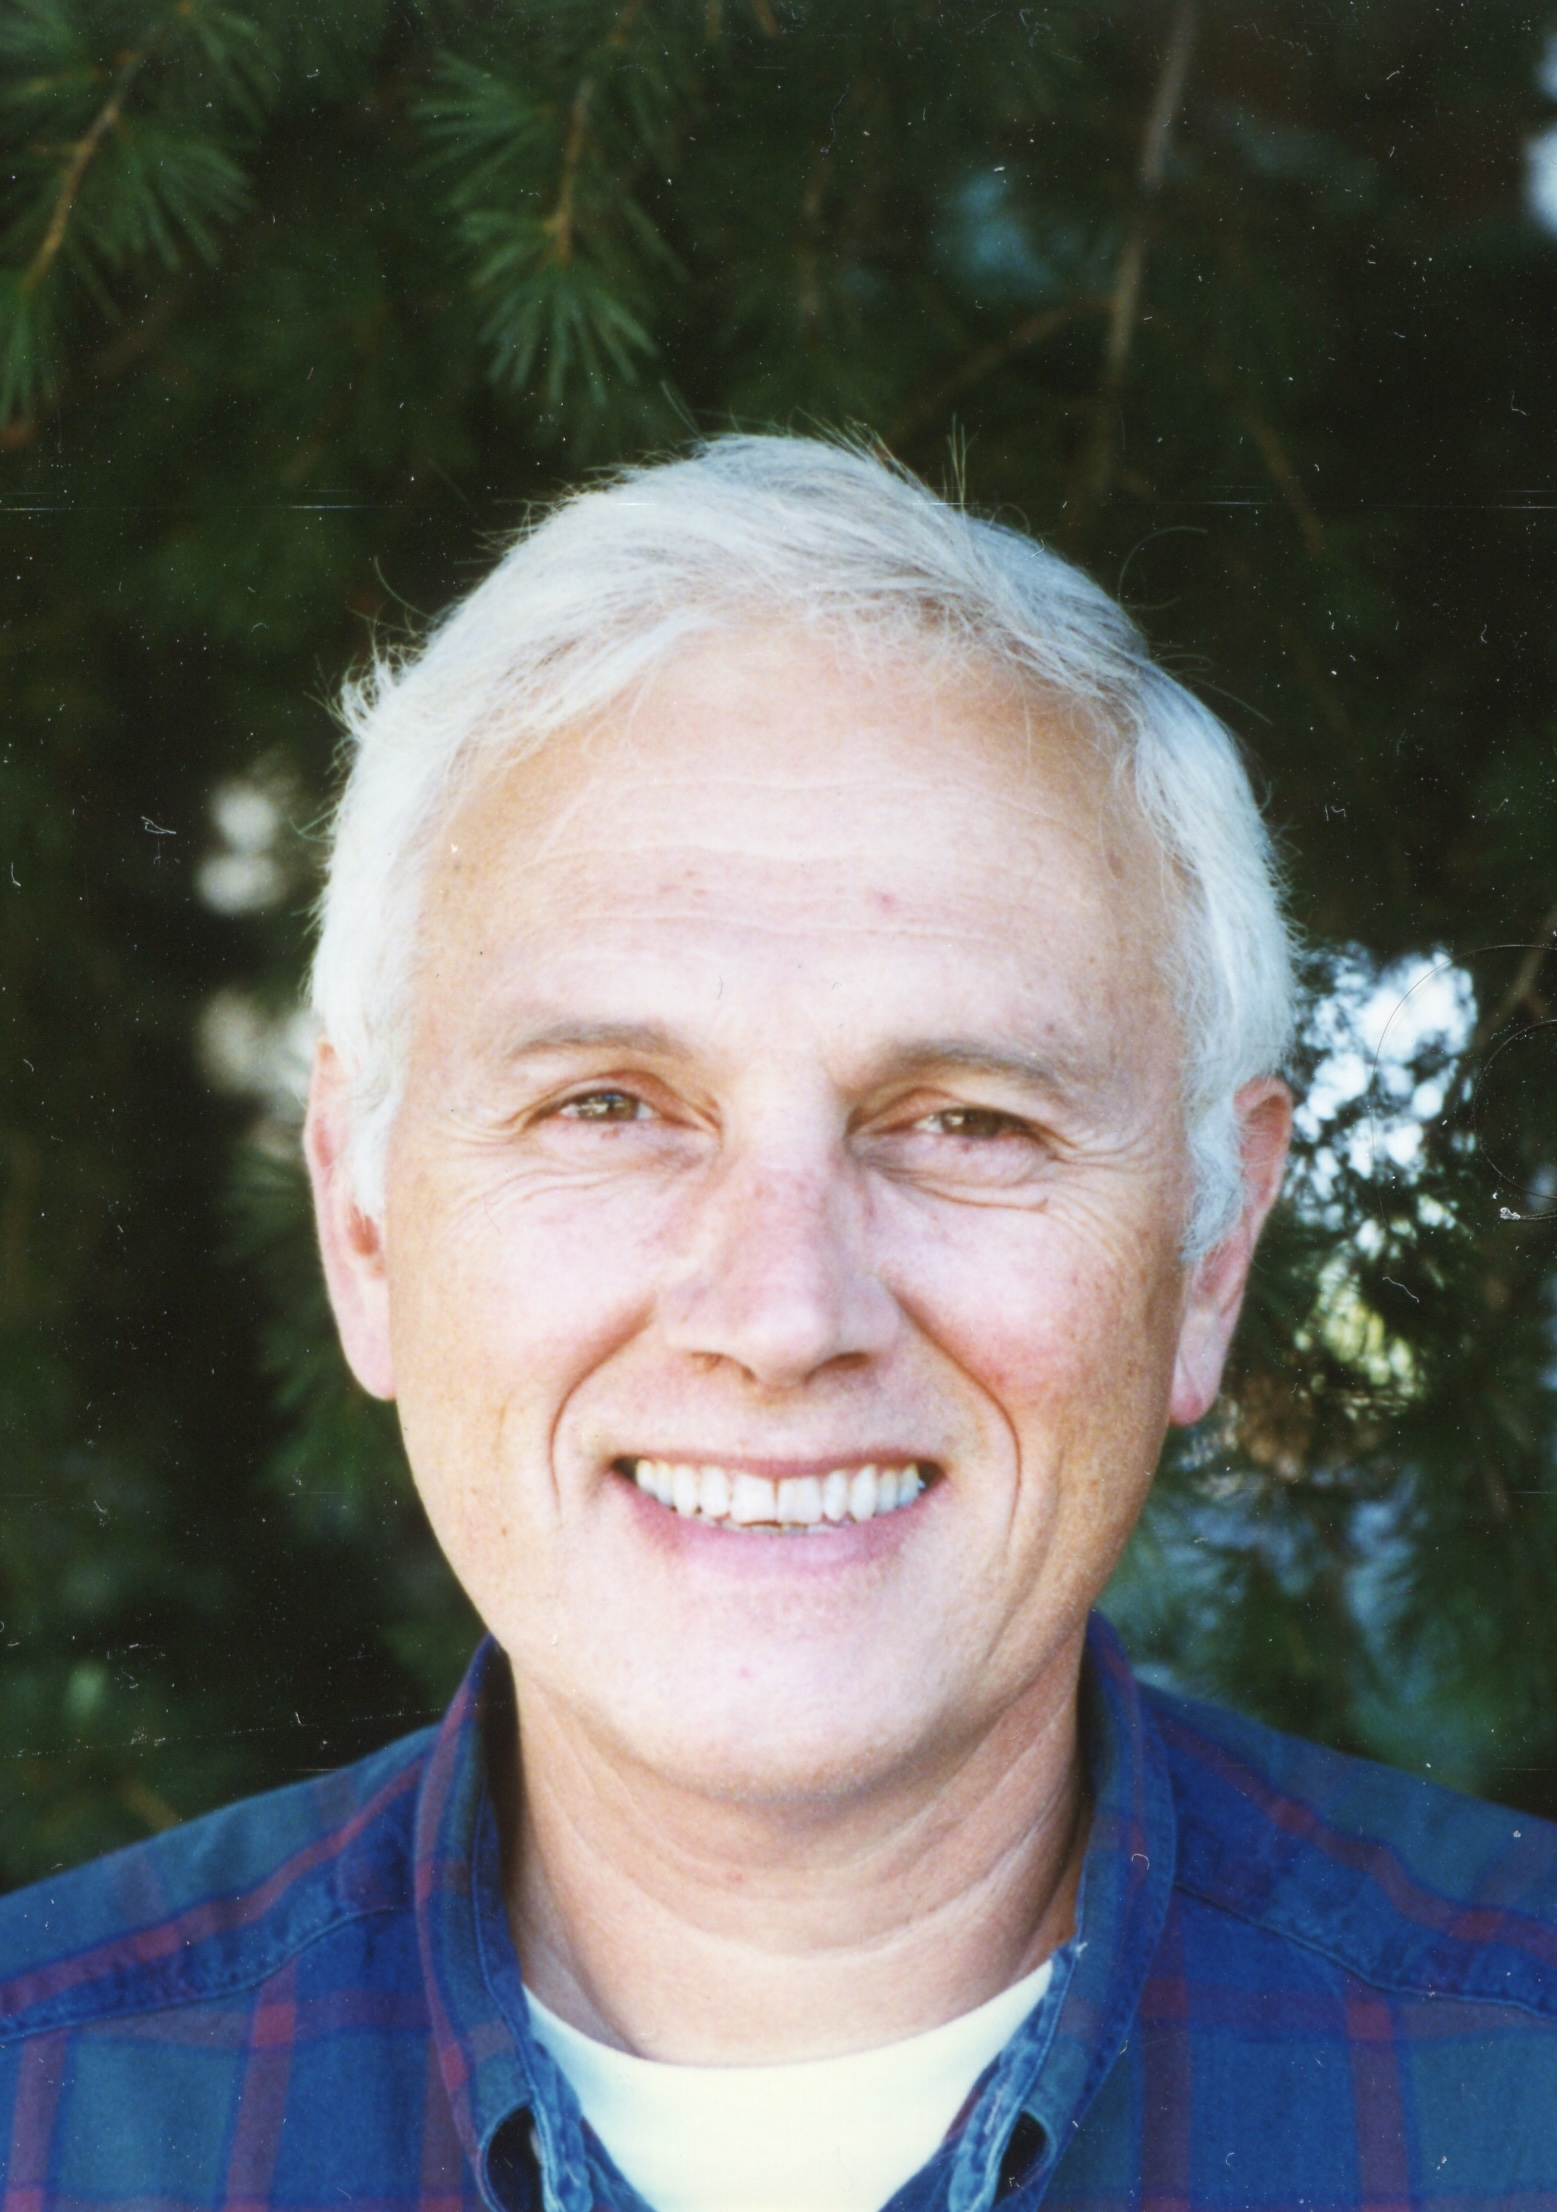
\includegraphics[width=\linewidth]{figures/mgcrandall.jpg}
    \captionof*{figure}{\tiny M.G.\ Crandall}
  \end{minipage}\vspace{-2ex}
    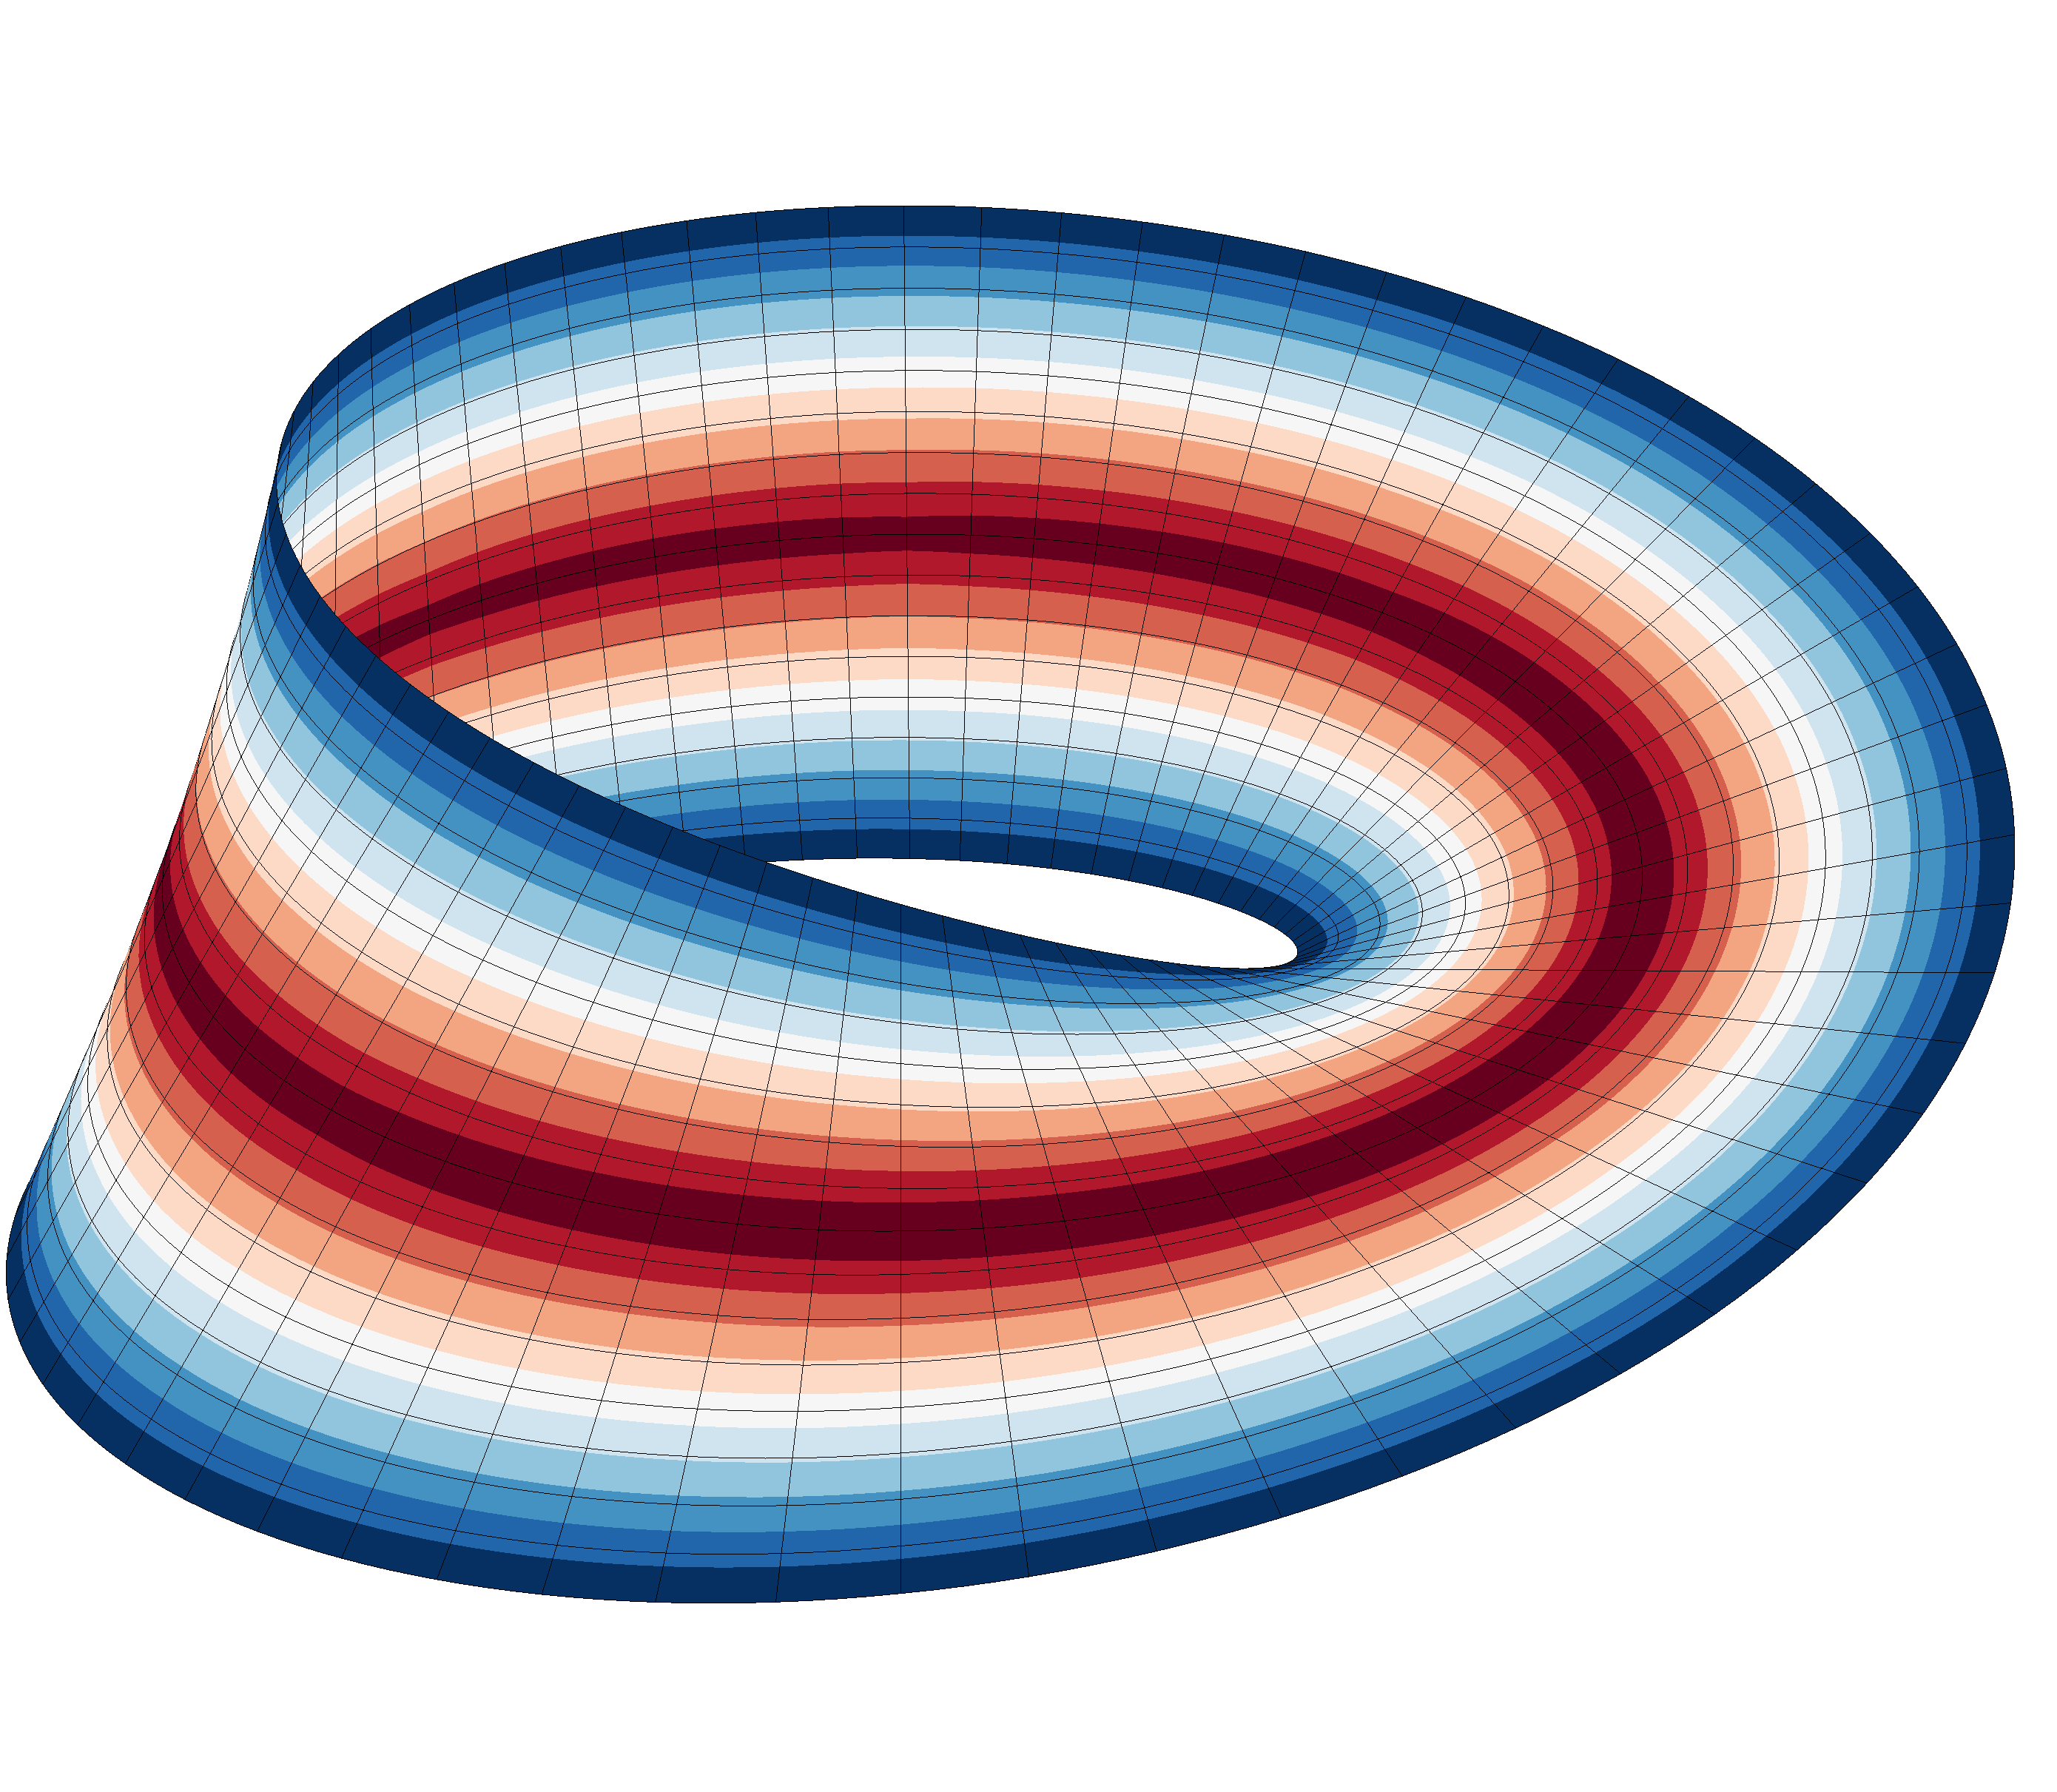
\includegraphics[width=0.7\linewidth]{figures/eikonal_mobius.png}
\end{figure}
\end{minipage}
\end{frame}




\begin{frame}\frametitle{An Example}
\begin{example}[Eikonal Equation]
Given $\Omega \subset \mathbb R^n$, a continuous function $\rho : \Omega \to \mathbb R$, and boundary data $g \in W^{1,\infty}(\Omega)$ such that $|\nabla g| \le \rho$,  find $u : \Omega \to \mathbb R$ such that
\begin{equation*}\label{eq:eik}
\aligned
|\nabla u| &= \rho \text{ in } \Omega,\\
u &= g \text{ on } \partial \Omega.
\endaligned
\end{equation*}
This equation admits a unique viscosity solution $\bar{u}$. \hypertarget{eikonal}{}
 \hyperlink{target_visc}{\beamerbutton{definition}}
\end{example}\visible<2->{
\begin{beamercolorbox}[rounded=true, shadow=true, wd=\textwidth]{block title}\centering
But what does this have to do with inequality constraints or variational inequalities?
\end{beamercolorbox}}

\end{frame}

\begin{frame}\frametitle{Gradient Constraints}
% \hypertarget{eikonal}{}  % Target anchor”
    % Button to go back
%    \hyperlink{extensions}{\beamerbutton{Back to Extensions}}
\begin{beamercolorbox}[rounded=true, shadow=true, wd=\textwidth]{block body}
$\Omega \subset \mathbb R^n$ is an open bounded subset.\medskip

$\rho : \Omega \to \mathbb R_+$ is continuous and $\rho \ge \underline{\rho} > 
0$ for constant $\underline{\rho}$ (a.e.\ $\Omega$).\medskip

Define an objective function
\[
J(v) := -\int_{\Omega} v \, \mathrm{d} x 
\] 
over
\[
K = \left\{
v \in W^{1,\infty}_g(\Omega) \left|\; | \nabla v | \le \rho \text{ a.e. } \Omega \right.
\right\}
\] 
where $g \in W^{1,\infty}(\Omega)$ satisfies the bound constraint.\medskip

Then $u$ the \alert{minimizer} of $J$ over $K$ is a \alert{viscosity solution} of the \alert{eikonal equation}.\footnote{\tiny S. Zagatti (2014)}
\end{beamercolorbox}

%S. Zagatti (2014)\footnote{\tiny Theorem 1., \textit{Maximal generalized solution of eikonal equation}  J. Differential Equations 257 (2014) 231–263 } if $\rho$ is continuous on $\Omega$ up to a closed null set $N$, then $u$ is a generalized solution of the \textbf{Eikonal equation}:
\end{frame}

\begin{frame}\frametitle{LVPP for Eikonal Equation}
\vspace{-1ex}
\begin{minipage}{0.25\textwidth}\scriptsize
\begin{beamercolorbox}[rounded=true, shadow=true, wd=\textwidth]{block title}
$V := H^1_0(\Omega)$\medskip

$B := \nabla$\medskip

$C := \mathbb B_{1}(0)$\medskip

$\Omega_d := \Omega$\medskip
 
$R(a) := -\sqrt{1 - \|a\|^2}$\medskip

$\rho := 1$\medskip

$\psi^0 := 0$
\end{beamercolorbox}
\end{minipage}\hfill\visible<2->{
\begin{minipage}{0.72\textwidth}  %%<--- here
\begin{beamercolorbox}[rounded=true, shadow=true, wd=\textwidth]{block body}
Find \only<2,3>{$(u^{k}, \psi^{k}) \in H^1_0(\Omega) \times L^2(\Omega,\mathbb{R}^n)$}\only<4->{satisfying $(u^{k}, \psi^{k}) \in L^2(\Omega) \times H(\operatorname{div},\Omega)$}
\only<2>{
\begin{subequations}
\label{eq:eikonal-lvpp-H1}
\begin{align*}
   -\alpha_k(1, v) +  (\psi^k - \psi^{k-1}, \nabla v)
    &= 0, \\
  (\nabla u^k, w) - \bigg(\frac{\psi^k}{\sqrt{1+|\psi^k|^2}}, w\bigg)
    &= 0,
\end{align*}
\end{subequations}}\only<3>{
\begin{subequations}
\label{eq:eikonal-lvpp-H1}
\begin{align*}
     \underbrace{-\alpha_k(1, v)}_{\scriptsize \alpha_k (J'(u^k),v)} +  \underbrace{(\psi^k - \psi^{k-1}, \nabla v)}_{\scriptsize \langle B^*(\psi^k - \psi^{k-1}),v\rangle}
    &= 0, \\
    \underbrace{(\nabla u^k, w)}_{\scriptsize (Bu^k,w)} - \underbrace{\bigg(\frac{\psi^k}{\sqrt{1+|\psi^k|^2}}, w\bigg)}_{\scriptsize (\nabla R^*(\psi^k),w)}
    &= 0,
\end{align*}
\end{subequations}}
\only<4->{
\begin{subequations}
\label{eq:eikonal-lvpp-Hdiv}
\begin{align*}
    \bigg(\frac{\psi^k}{\sqrt{1+|\psi^k|^2}}, w\bigg) + (u^k, \nabla\cdot w)
    &= 0,
\label{eq:eikonal-lvpp-Hdiv-1}
    \\
    (\nabla\cdot \psi^k, v)
    &= 
    (\nabla\cdot\psi^{k-1},v) - \alpha_k(1,v),
\label{eq:eikonal-lvpp-Hdiv-2}
\end{align*}
\end{subequations}}
for all \only<2,3>{$(v,w) \in H^1_0(\Omega) \times L^2(\Omega,\mathbb{R}^n)$}\only<4->{for all $(v,w) \in L^2(\Omega) \times H(\operatorname{div},\Omega)$}.\end{beamercolorbox}
\end{minipage}}

\visible<4->{
\begin{beamercolorbox}[rounded=true, shadow=true, wd=\textwidth]{block title}\centering
Despite not being originally in divergence form, we have a new, meaningful weak formulation. This allows seamless integration with popular finite element software.
\end{beamercolorbox}}
\end{frame}

\begin{frame}\frametitle{LVPP for Eikonal Equation}
\begin{beamercolorbox}[rounded=true, shadow=true, wd=\textwidth]{block body}
We consider three different domains:
\begin{itemize}
\item a two-dimensional star-shaped domain,
\item a solid (three-dimensional) sphere,
\item a M\"obius strip.
\end{itemize}
Domains are scaled so that the maximum shortest distance to boundary is one.\medskip

\textbf{Finite element spaces}
\begin{itemize}
\item Star-shaped and sphere: We used a first-order discontinuous piecewise polynomial space for $L^2(\Omega)$ and second-order Raviart--Thomas polynomial space for $H(\operatorname{div},\Omega)$.\footnote{\tiny This is the standard choice for Darcy flow problems.}
\item M\"obius strip: We used a continuous piecewise polynomial discretization of Taylor--Hood-type. In particular, we used second-order Lagrange elements to approximate $\psi^k$ and first-order Lagrange elements for $u^k$.
\end{itemize}
\end{beamercolorbox}
\end{frame}

\begin{frame}\frametitle{LVPP for Eikonal Equation}
\begin{minipage}{0.35\linewidth}
\begin{beamercolorbox}[rounded=true, shadow=true, wd=\textwidth]{block body}
 \visible<1->{We solved each discretized subproblem with a damped Newton method.} \medskip
 
 \visible<1->{$\alpha_k = 10\cdot\min\{2^k, 5\}$\medskip}

Stop proximal steps when $\|u^k - u^{k-1}\|_{L^2(\Omega)} < 10^{-4}$.
\end{beamercolorbox}
\visible<2->{
\begin{beamercolorbox}[rounded=true, shadow=true, wd=\textwidth]{block title}
Performance of LVPP:\\
Max.\ no.\ Newton steps: 3\\
Total Newton steps $< 10$\\
(For all three examples)
\end{beamercolorbox}}
\end{minipage}\hspace{0ex}
\begin{minipage}{0.6\linewidth}
 \centering
\begin{figure}
\centering
    \subcaptionbox*{} {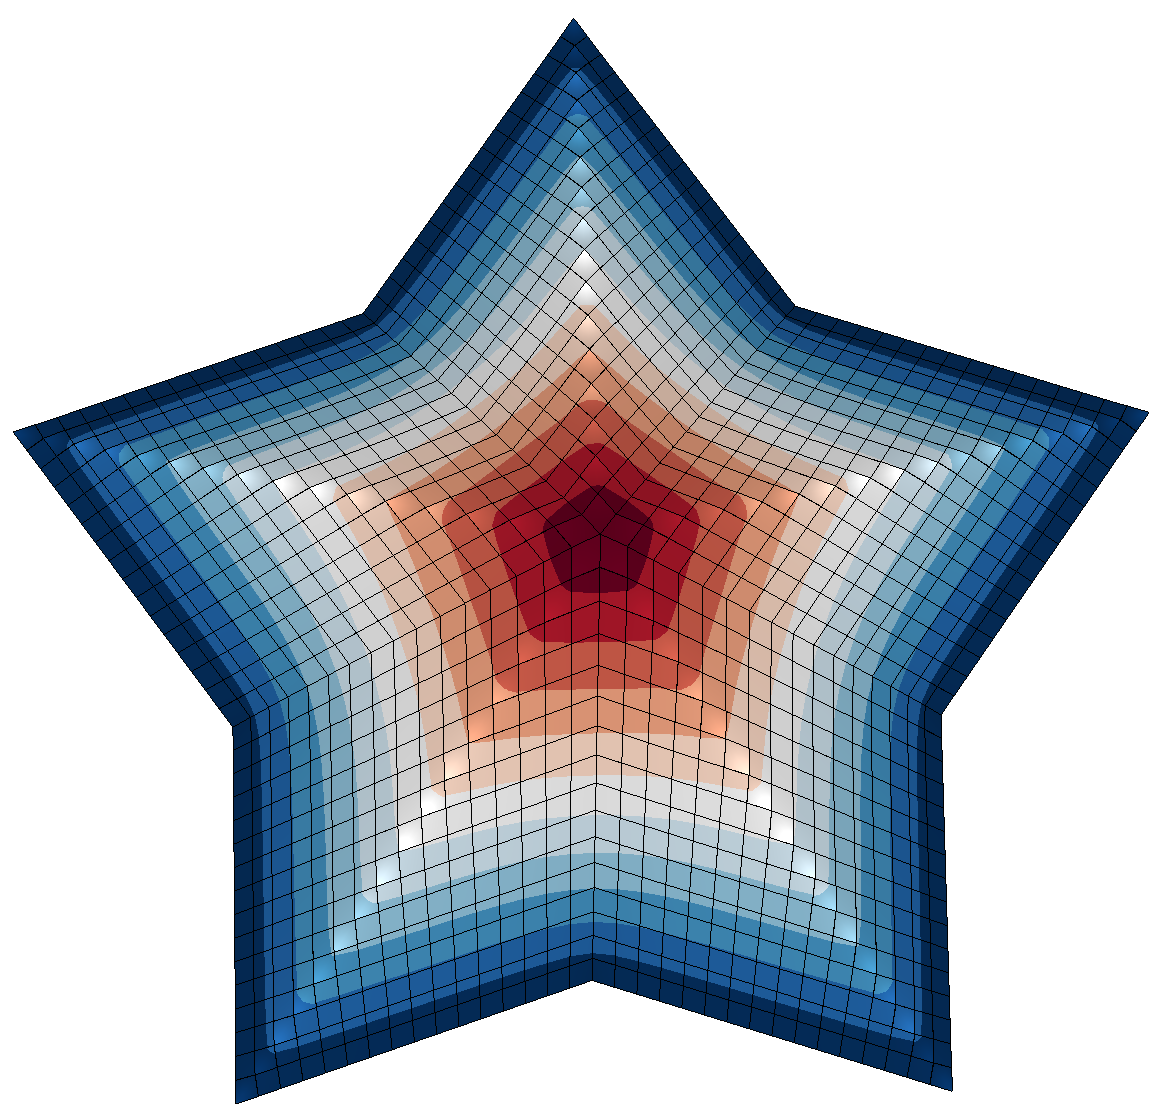
\includegraphics[width=0.29\linewidth]{figures/Eikonal.png}}
    \subcaptionbox*{} {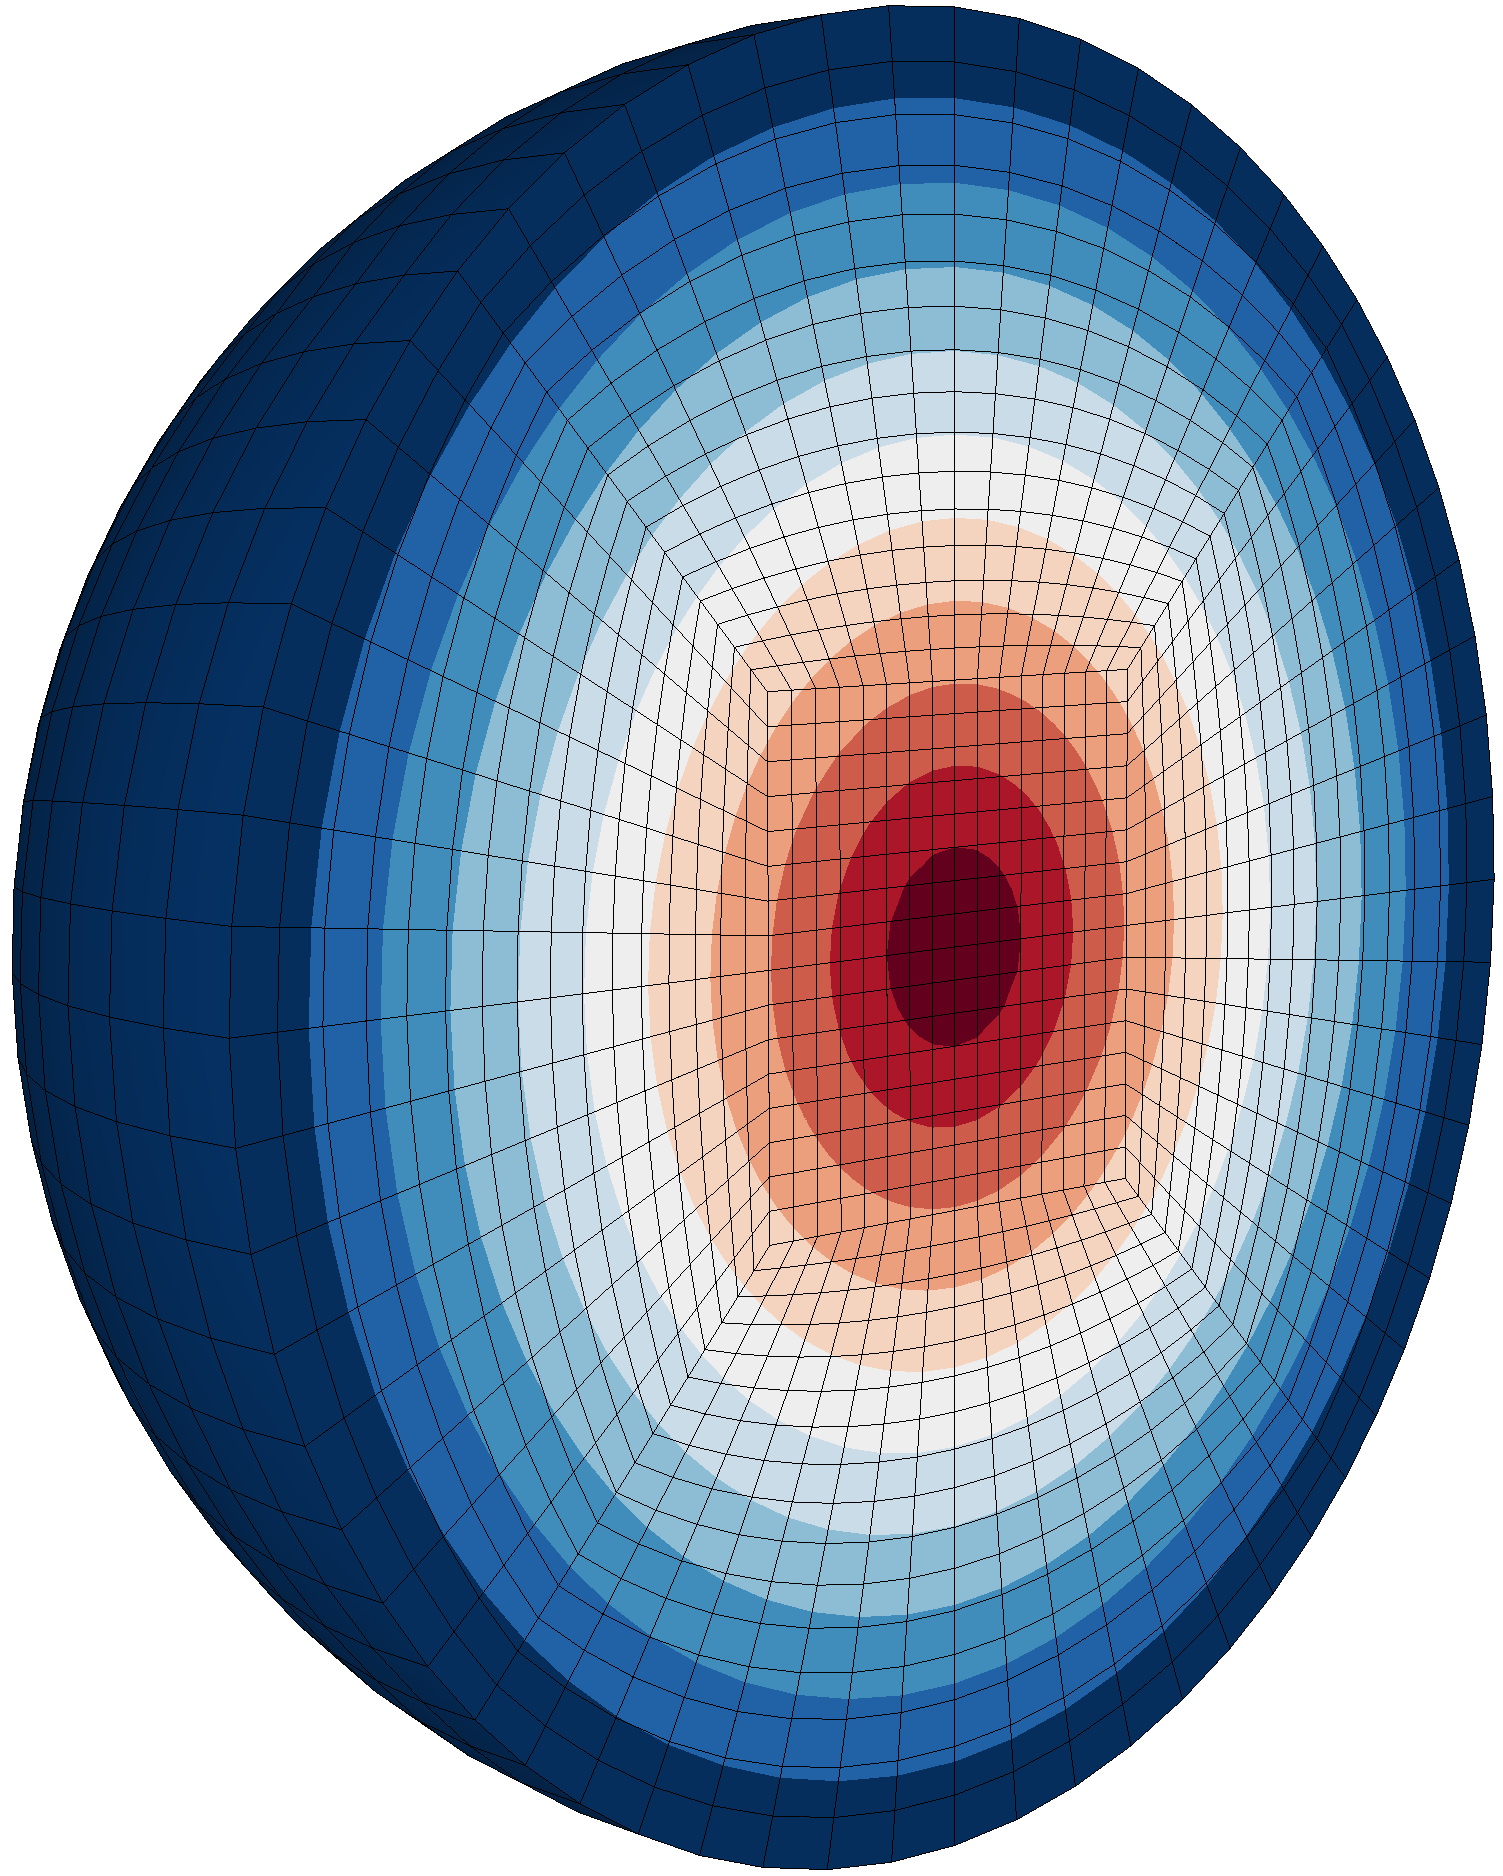
\includegraphics[width=0.23\linewidth]{figures/eikonal_sphere.png}}
    \subcaptionbox*{} {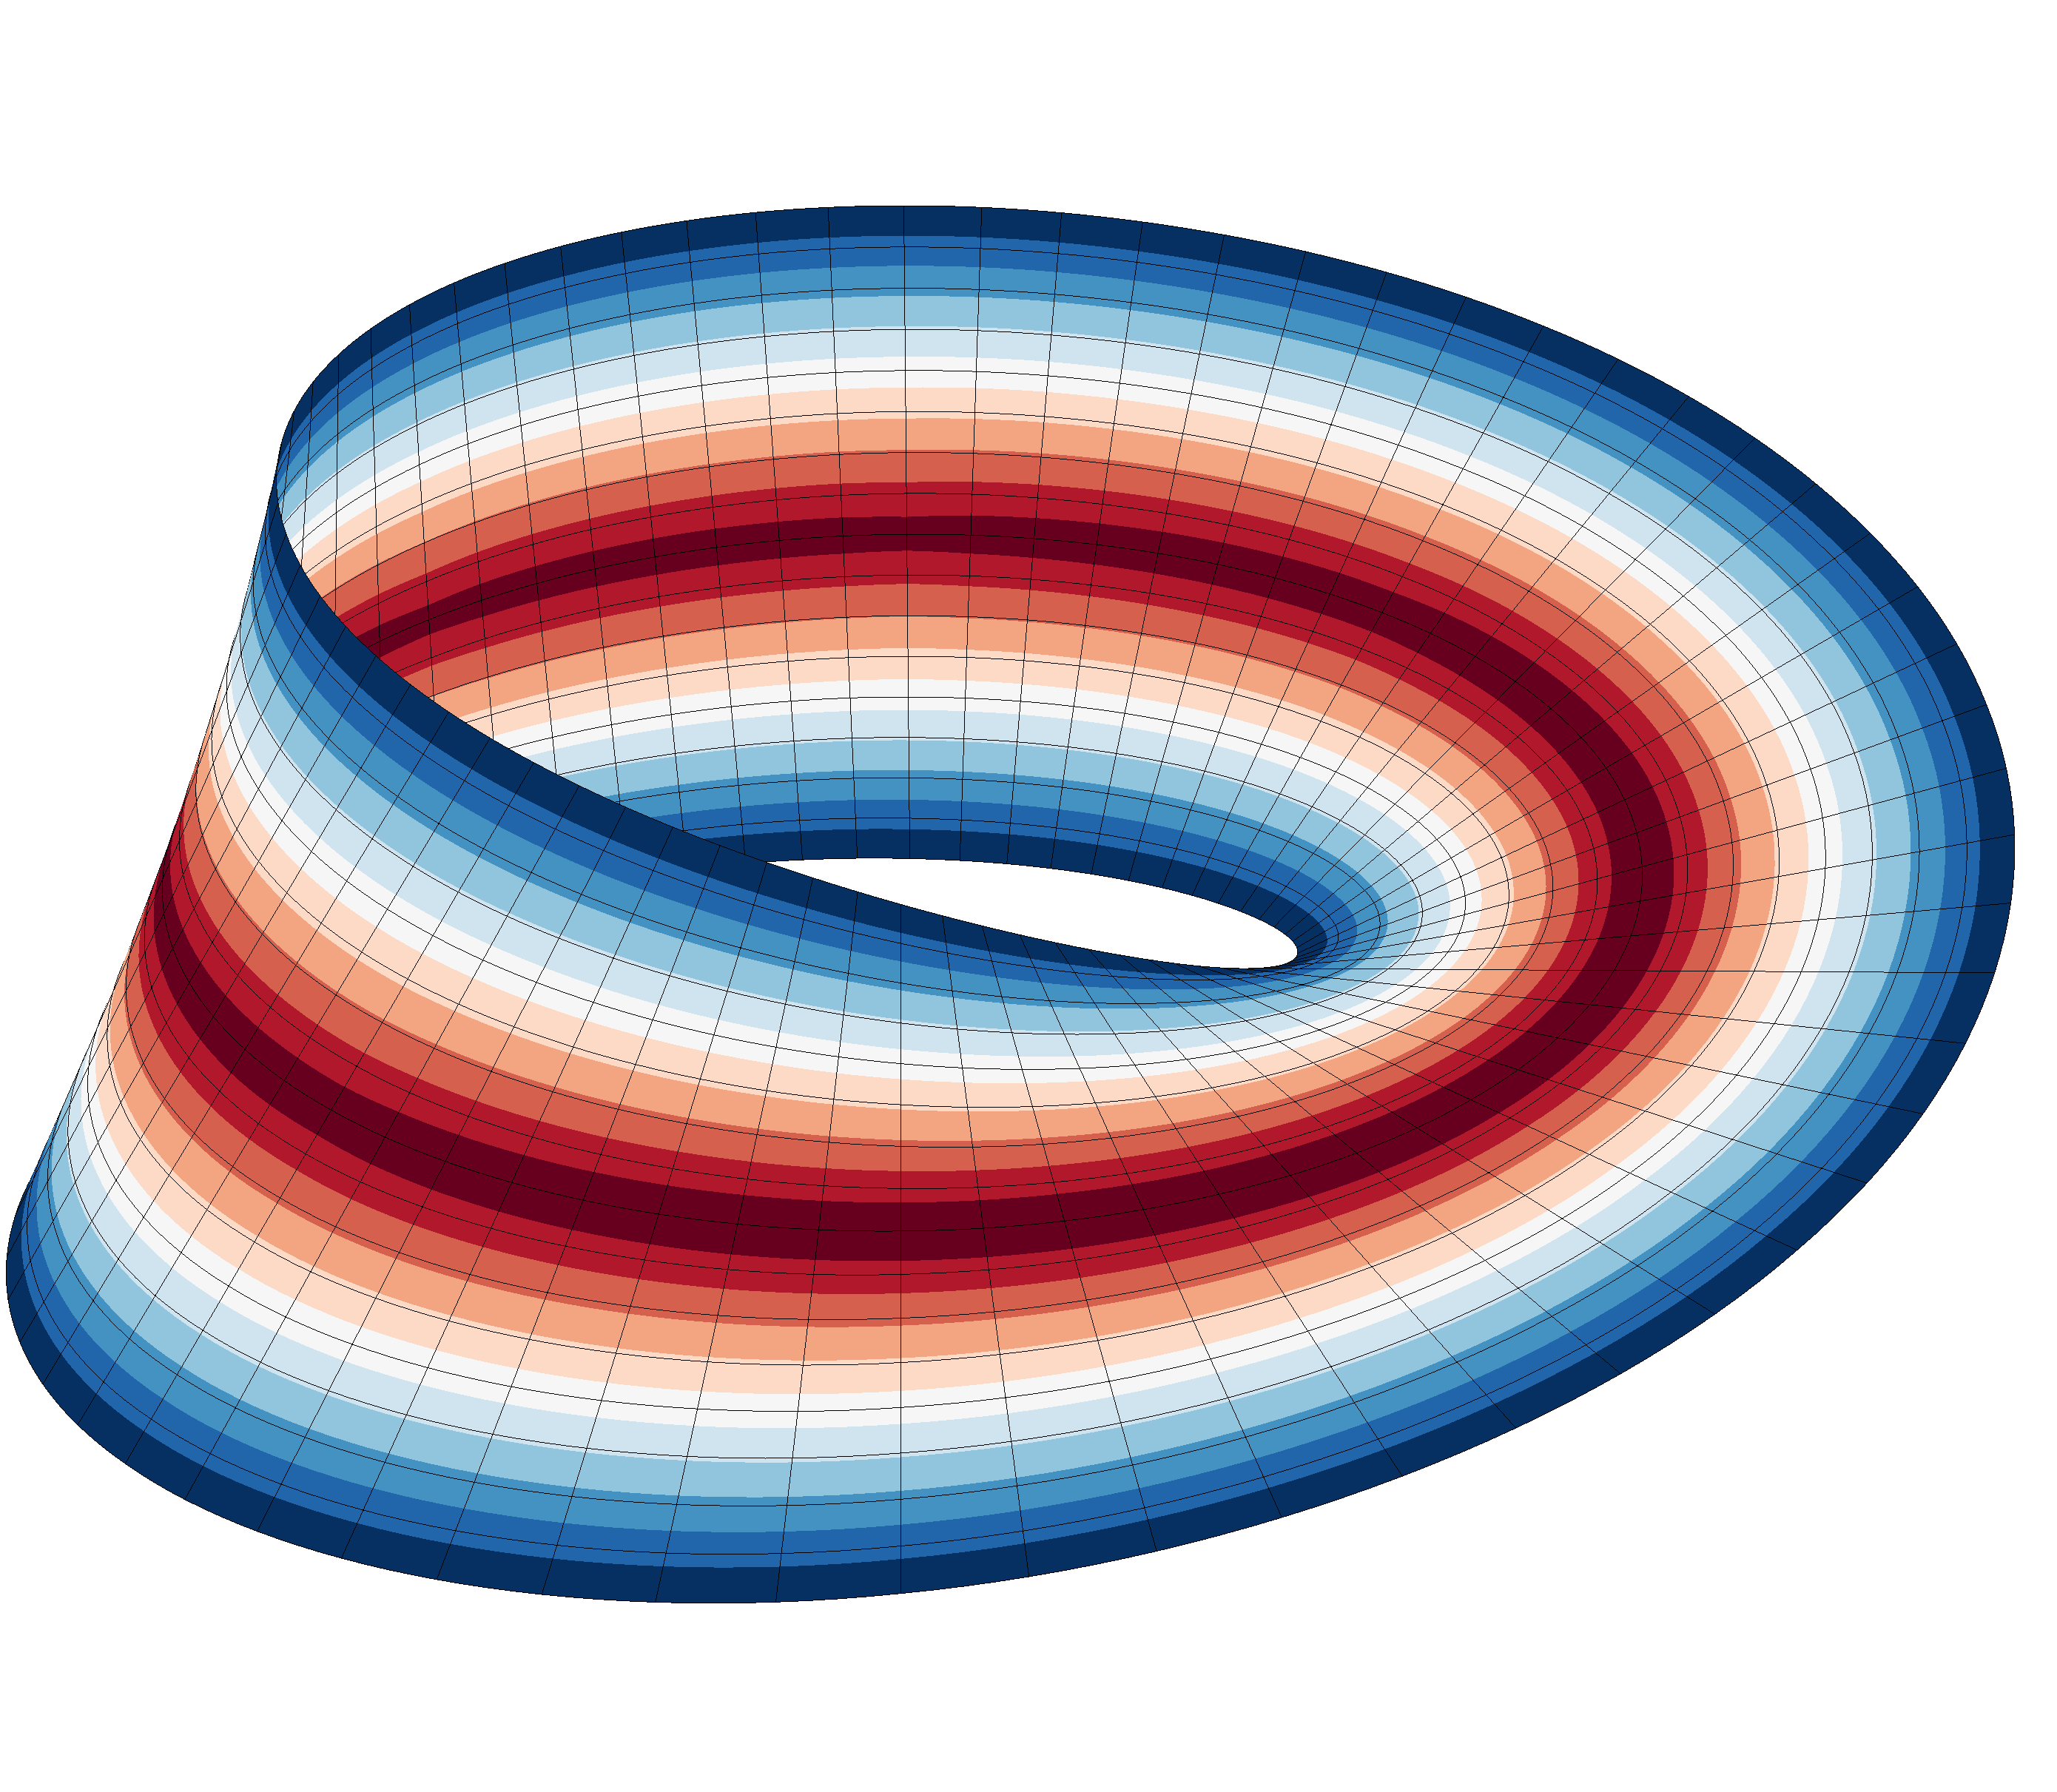
\includegraphics[width=0.29\linewidth]{figures/eikonal_mobius.png}}
\end{figure}\visible<3->{
\begin{minipage}{0.9\textwidth}
\begin{beamercolorbox}[rounded=true, shadow=true, wd=\textwidth]{block body}
Nothing can beat Sethian's and Osher's Fast Marching and Fast Sweeping methods in computational complexity, but LVPP allows for easy integration in complex finite element codes.
\end{beamercolorbox}
\end{minipage}}
\end{minipage}
\end{frame}

\begin{frame}\frametitle{Conclusion and Outlook}
\begin{beamercolorbox}[rounded=true, shadow=true, wd=\textwidth]{block body}
\visible<1->{Starting with convex optimization, we \only<1>{(formally!)}\only<2->{\alert{(formally!)}} derived a new kind of saddle point problem that provides a unifying perspective on variational inequalities and beyond.
}\medskip

\visible<2->{
\alert{HOWEVER}, the general LVPP framework requires \textbf{rigorous} justification beyond simple bound constraints. }\visible<3->{This includes: 
\begin{itemize}
\item Regularity theory of solutions to the LVPP subproblems 
\item Differentiability of Nemitskii operators generated by $\nabla R^*$
\item Justification of Newton on continuous and discrete levels
\item Need iterative solvers for the new saddle point problems
\item Proofs of mesh and order independence.
\end{itemize}
}

\visible<4->{
But the \textbf{extensive numerical studies} indicate it is worth the effort!
}
\end{beamercolorbox}
\end{frame}

%\begin{frame}\frametitle{Summary}
%\begin{beamercolorbox}[rounded=true, shadow=true, wd=\textwidth]{block body}
%\begin{enumerate}
%\item Starting with a classical problem from the theory of linear elliptic partial differential equations, we introduced the Direct Method of the Calculus of Variations.
%\item By restricting the solution space to pointwise inequality constraints, we motivated the necessity of the study of variational inequalities, which enjoy a wide array of interesting applications.
%\item We introduced the Obstacle Problem for the first time in order to understand how to derive variational inequalities and prove existence and uniqueness of solutions.
%\item Lagrange Multipliers were introduced to highlight the differences  to the theory of PDEs and linearly constrained variational problems. The low regularity of the Lagrange multiplier was discussed.
%\item The issues of poor scaling, mesh independence, and a lack of global bound preservation of naive solution algorithms is discussed.
%\end{enumerate}
%\end{beamercolorbox}
%\end{frame}

% \begin{frame}{Frame Title}
    
% \end{frame}
% \begin{frame}{Frame Title}
    
% \end{frame}
% \begin{frame}{Frame Title}
    
% \end{frame}
% \subsection{}
% \begin{frame}{Frame Title}
    
% \end{frame}
% \begin{frame}{Frame Title}
    
% \end{frame}
% \begin{frame}{Frame Title}
    
% \end{frame}
% \begin{frame}{Frame Title}
    
% \end{frame}
% \begin{frame}{Frame Title}
    
% \end{frame}
% \subsection{}
% \begin{frame}{Frame Title}
    
% \end{frame}
% \begin{frame}{Frame Title}
    
% \end{frame}
% \begin{frame}{Frame Title}
    
% \end{frame}
% \begin{frame}{Frame Title}
    
% \end{frame}

\begin{frame}\frametitle{SURE-AI}
\begin{minipage}{0.45\linewidth}
%  
\includegraphics[width=\linewidth]{figures/ai-centres.jpeg}
   
\includegraphics[width=\linewidth]{figures/result_superimposed.jpg} 
\end{minipage}%
\begin{minipage}{0.47\linewidth}
\begin{beamercolorbox}[rounded=true, shadow=true, wd=\textwidth]{block title}
%  \begin{itemize}
%    \item 
    \textbf{SU}stainable, \textbf{R}isk-averse, \textbf{E}thical AI\medskip
%    \item 

    One of six national AI centres funded by the Research Council of Norway\medskip
%    \item 

    Total budget: $>$ 290 million NOK \medskip
    
%    \item 
    Funding for 25 PhD/postdoctoral fellows, conferences, summer schools, and more.
%  \end{itemize}
  \end{beamercolorbox}
\end{minipage}
\begin{beamercolorbox}[rounded=true, shadow=true, wd=\textwidth]{block body}\scriptsize
 The focus of the center is to develop new AI technologies starting from the \textbf{basic mathematical methodologies} that will ensure reduced energy consumption, awareness to risk and ethicial considerations.\medskip

Among the many partners are Simula, BI, University of Oslo (UiO), NTNU, UiT, CICERO, Norges Bank Investment Management, Dolphin, Rystad Energy, Rema 1000 and several others.
  \end{beamercolorbox}
\end{frame}

 \appendix

\begin{frame}{Viscosity Solutions}
%\begin{definition}
\visible<1->{\textbf{Subsolution:} An \alert{upper semicontinuous} function $u$ in $\Omega$ is a \alert{viscosity subsolution} if for any $x_0 \in \Omega$ and any $C^2$ function $\phi$ such that $\phi(x_0) = u(x_0)$ and $\phi \geq u$ in a neighborhood of $x_0$, we have:
\[
F\left(x_0, \phi(x_0), D\phi(x_0)\right) \leq 0.
\]}\vspace{-1ex}

%\vspace{0.5em}

\visible<2->{\textbf{Supersolution:} A \alert{lower semicontinuous} function $u$ in $\Omega$ is a \alert{viscosity supersolution} if for any $x_0 \in \Omega$ and any $C^2$ function $\phi$
such that $\phi(x_0) = u(x_0)$ and $\phi \leq u$ in a neighborhood of $x_0$, we have:
\[
F\left(x_0, \phi(x_0), D\phi(x_0))\right) \geq 0.
\]}\vspace{-1ex}

%\vspace{0.5em}

\visible<3->{\textbf{Viscosity Solution:} A \alert{continuous} function $u$ is a \alert{viscosity solution} of the PDE
\[
F(x, u, Du) = 0 \quad \text{in } \Omega
\]
if it is both a subsolution and a supersolution. 
 \hypertarget{target_visc}{}
 \hyperlink{eikonal}{\beamerbutton{go back to eikonal}}
}
%\end{definition}
\end{frame}

\begin{frame}{Variational Fracture}

  \begin{minipage}{0.53\textwidth}
  \begin{beamercolorbox}[rounded=true, shadow=true, wd=\textwidth]{block title}\scriptsize
A.\ A.\ Griffith's foundational paper (1921) uses a preexisting crack and well-defined crack path.\medskip

Mostly overcome in the seminal work by Francfort and Marigo (1998)\medskip

The widely used \textbf{phase-field approximation} by Bourdin, Francfort, and Marigo (2000).
%\footnote{\tiny The model in Bourdin, Francfort, and Marigo (2000) is an Ambrosio-Tortorelli approximation of the Mumford-Shah functional \cite{Mumford1989,Ambrosio1990}.}

%We only solve for the vertical displacements here. 
     \end{beamercolorbox}
 
 \visible<2->{    
\begin{beamercolorbox}[rounded=true, shadow=true, wd=\textwidth]{block body}\scriptsize
\visible<2->{Challenge 1: Variational fracture is a \alert{free discontinuity problem (FDP)}. The state is split into a \alert{function} $u$ over $\Omega$ and a \alert{geometric quantity} $\Gamma \subset \Omega$.\medskip}
 
 \visible<3->{Challenge 2: The phase-field approximation has a \alert{non-convex energy} and admits \alert{non-unique global solutions}. \medskip}
 
 \visible<4->{Challenge 3: The \alert{irreversibility} of the crack evolution has to be built into the pointwise inequality constraints.}
      \end{beamercolorbox}}
    \end{minipage}\hspace*{1.75cm}
    \begin{minipage}{0.3\textwidth}
  \centering
 \begin{figure}
  \centering\vspace{1ex}
   \begin{minipage}[b]{0.4\textwidth}
    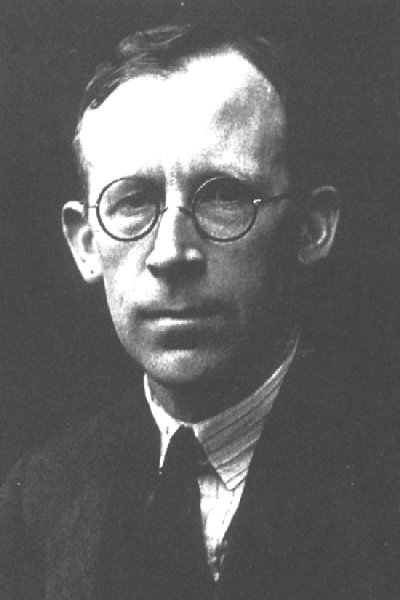
\includegraphics[width=\linewidth]{figures/griffith.jpg}
    \captionof*{figure}{\tiny A.A.\ Griffith}
  \end{minipage}
  \hfill
  \begin{minipage}[b]{0.4\textwidth}
    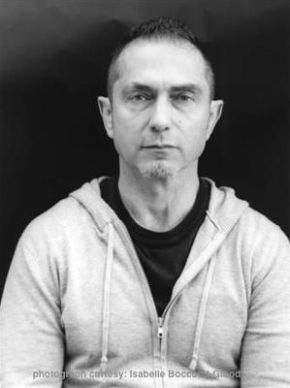
\includegraphics[width=\linewidth]{figures/francfort.jpg}
    \captionof*{figure}{\tiny G.\ Francfort }
  \end{minipage}
  \vspace{1em}
  \begin{minipage}[b]{0.4\textwidth}
    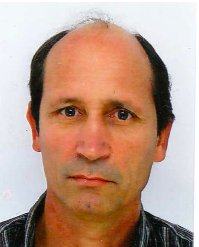
\includegraphics[width=\linewidth]{figures/marigo.jpeg}
    \captionof*{figure}{\tiny J.-J.\ Marigo}
  \end{minipage}
  \hfill
  \begin{minipage}[b]{0.4\textwidth}
    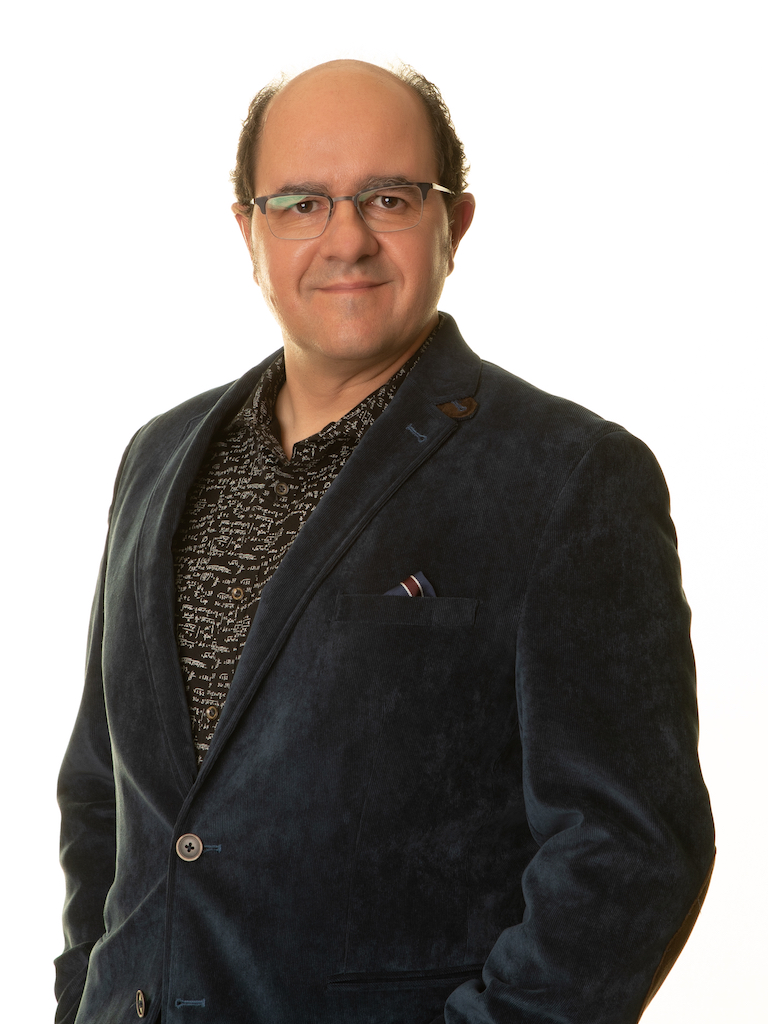
\includegraphics[width=\linewidth]{figures/BlaiseBourdin_1024.jpg}
    \captionof*{figure}{\tiny B.\ Bourdin }
  \end{minipage}
\end{figure}
    \end{minipage}
\end{frame}

\begin{frame}\frametitle{Problem Description}
\begin{minipage}{0.6\textwidth}
\begin{beamercolorbox}[rounded=true, shadow=true, wd=\textwidth]{block body}\scriptsize
Domain: $\Omega \subset \mathbb R^n$ open, bounded set\medskip 

\visible<2->{(Francfort \& Marigo): $u : \Omega \to \mathbb R$ (displacement), $\Gamma \subset \Omega \cap \mathbb R^{n-1}$ (crack). Note \alert{this is not a function!}\medskip}

\visible<3->{(Bourdin, Francfort \& Marigo): The \alert{geometric variable} $\Gamma$ is replaced by an \alert{order parameter} $c : \Omega \to [0,1]$ 
\[
c = 0 \text{ no damage, } \alert{c = 1} \text{ presence of crack.}
\] 
The localization of the crack controlled by a \alert{length scale} $\ell > 0$ \medskip}

\visible<4->{The crack evolution is computed over a \alert{quasi-static incremental loading} procedure.\medskip}

\visible<5->{At each step, the load on the body is varied, and the body is allowed to equilibrate.\medskip}
\end{beamercolorbox}
\end{minipage}\hspace{4ex}
\begin{minipage}{0.27\textwidth}
\begin{figure}
  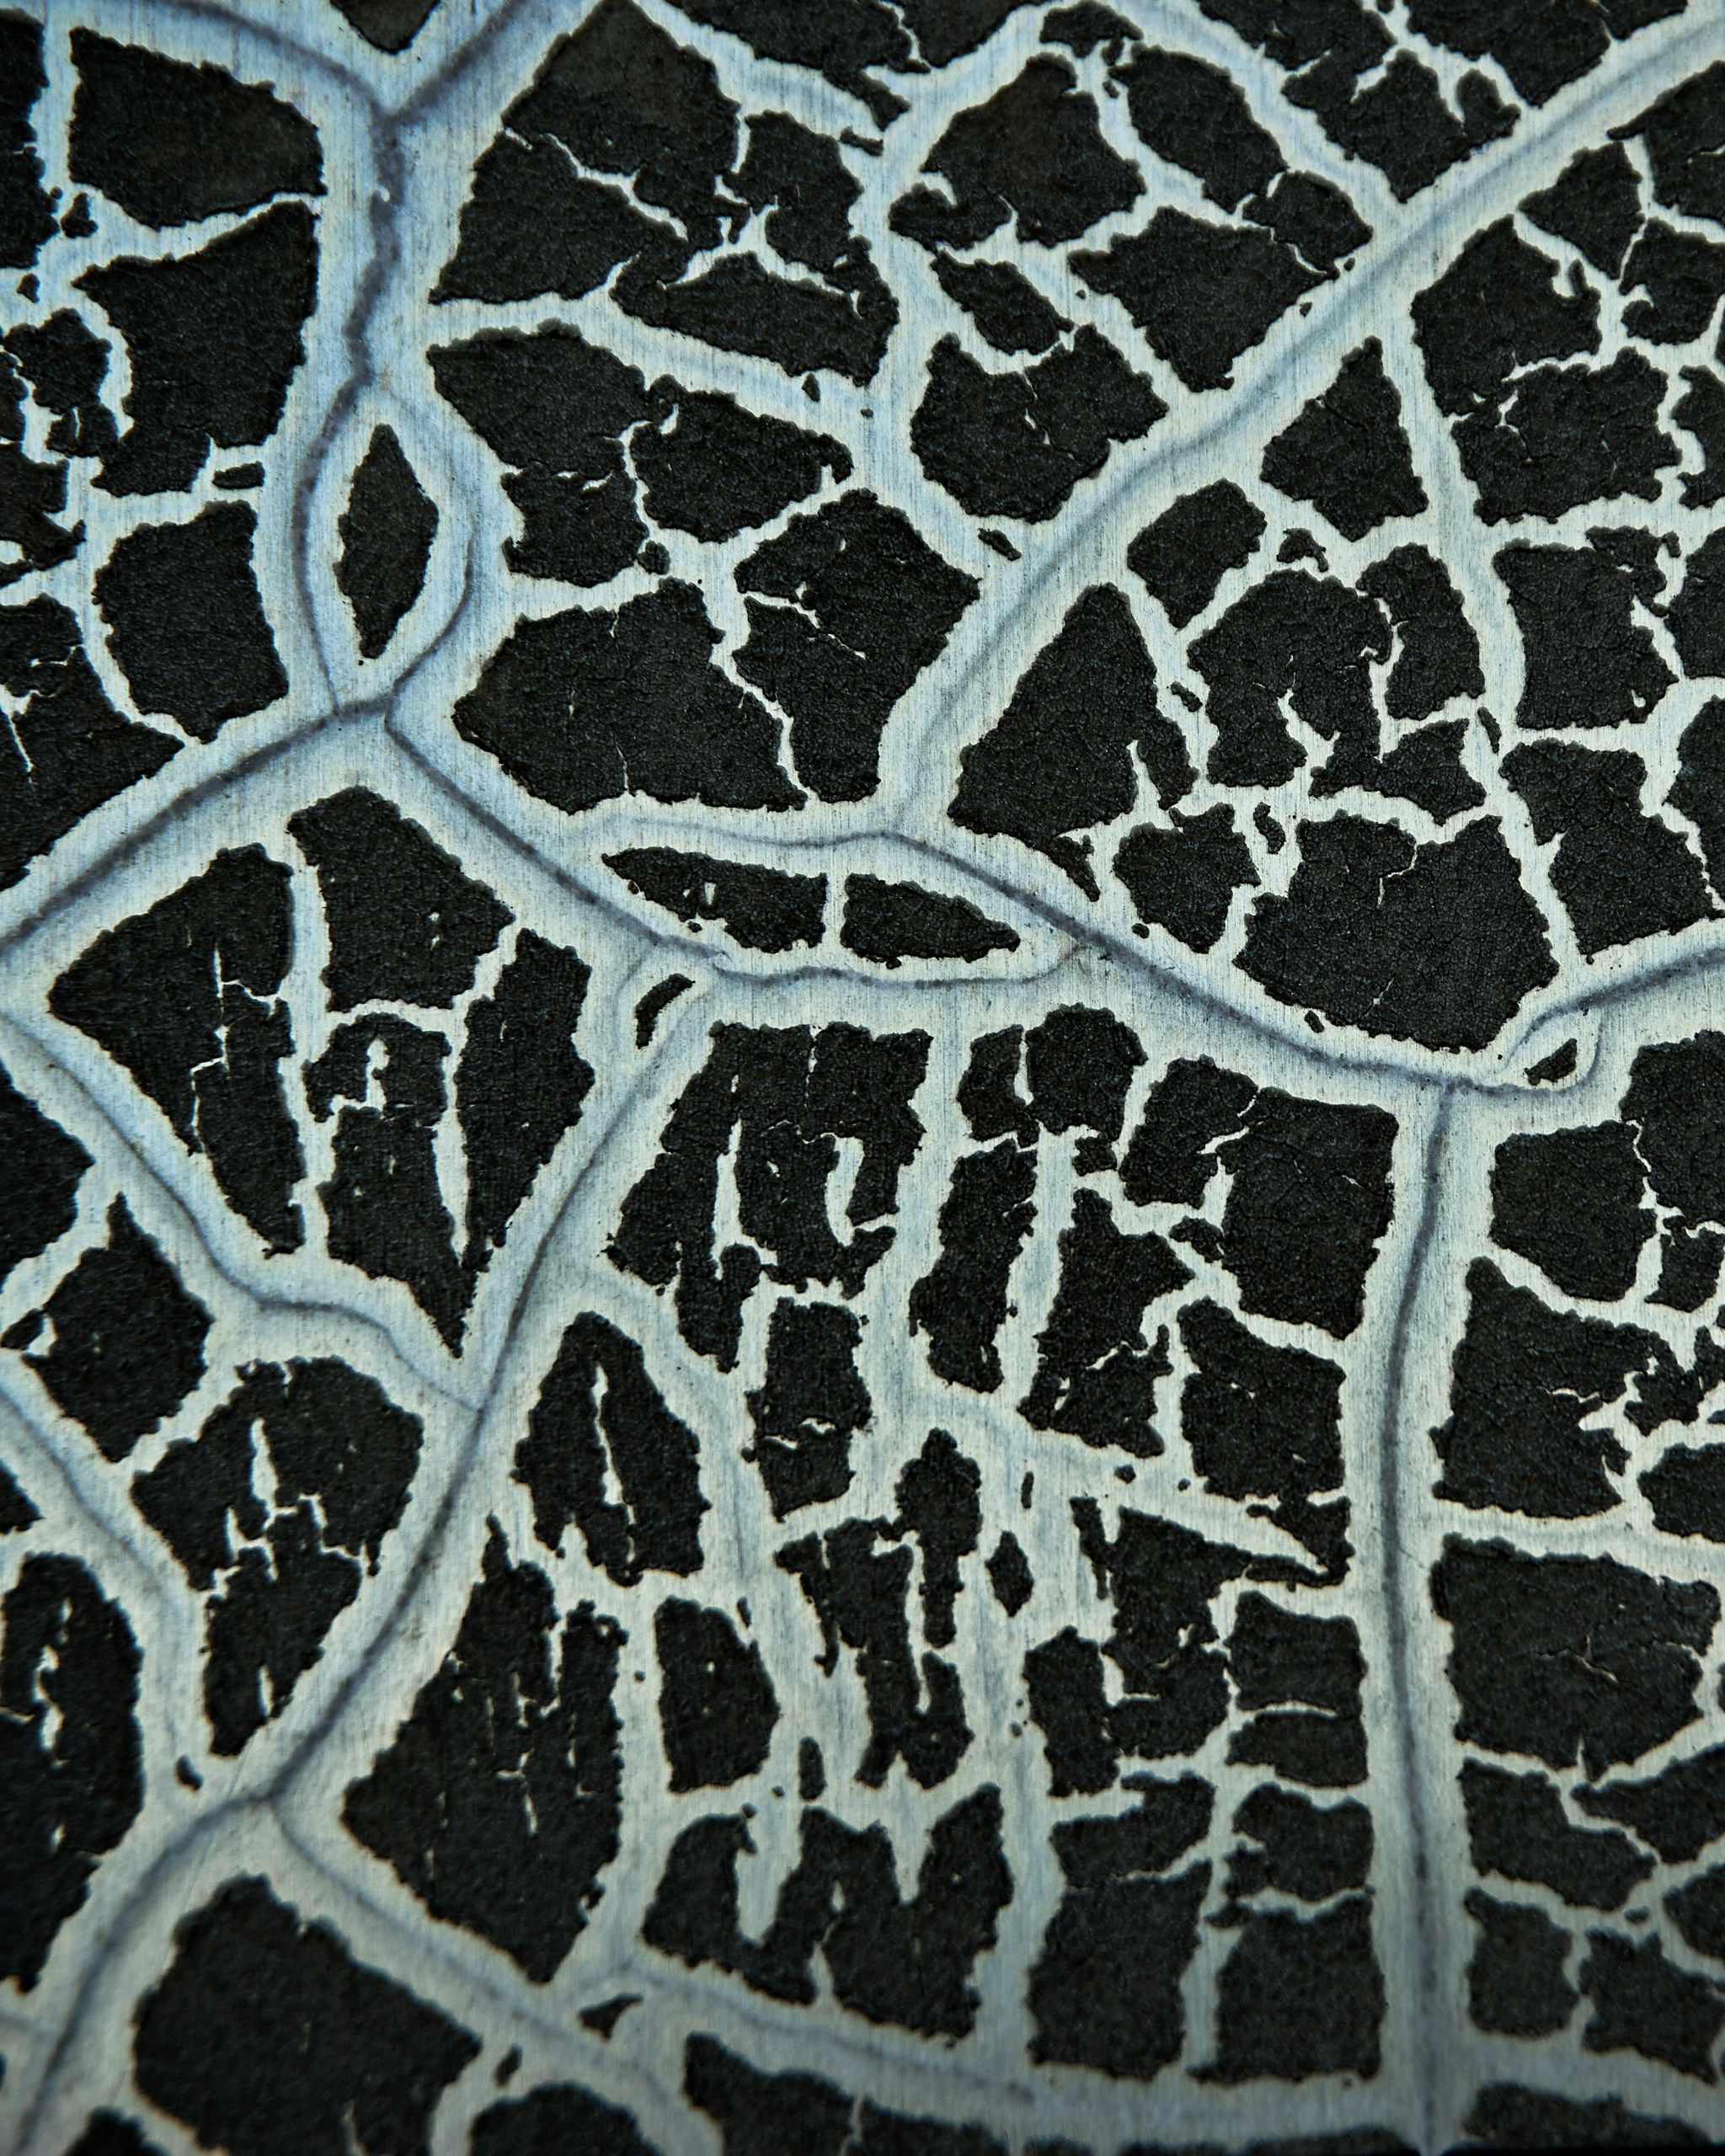
\includegraphics[width=\linewidth]{figures/christian-lambert-KtqTxJgN70M-unsplash.jpg}
  \captionof*{figure}{\tiny Photo by Christian Lambert}
  \end{figure}
\end{minipage}

%%Photo by <a href="https://unsplash.com/@_christianlambert?utm_content=creditCopyText&utm_medium=referral&utm_source=unsplash">Christian Lambert</a> on <a href="https://unsplash.com/photos/blue-and-white-abstract-painting-KtqTxJgN70M?utm_content=creditCopyText&utm_medium=referral&utm_source=unsplash">Unsplash</a>
      
\end{frame}

\begin{frame}\frametitle{Problem Description}
\begin{beamercolorbox}[rounded=true, shadow=true, wd=\textwidth]{block body}
At each loading step, we are given Dirichlet boundary data $g$ and the previous order parameter $c_{\rm prev}$. \visible<2->{This defines our feasible set $K$:
\begin{equation*}
\label{eq:FeasibleSetFracture}
K = \left\{ (u,c) \in H^1_g(\Omega) \times H^1(\Omega) \mid 0 \le c_{\rm prev} \le c \le 1 \; \text{a.e.~in} \; \Omega \right\},
\end{equation*}
where
%\begin{equation*}
$V = H^1_g(\Omega) = \left\{ u \in H^1(\Omega) \mid \gamma u = g \text{ on } \Gamma_D \right\},$
%\end{equation*}
with $\Gamma_D \subset \partial \Omega$.}
\end{beamercolorbox}

\visible<3->{
\begin{beamercolorbox}[rounded=true, shadow=true, wd=\textwidth]{block body}
Given energy release rates $G_c > 0$, 
%the length scale $\ell > 0$,  
%an artificial residual stiffness
artificial  stiffness
%of a fully ruptured phase 
$\epsilon > 0$, we arrive at the (\alert{non-convex}) objective functional:
\[
J(u,c) := \underbrace{\frac{1}{2}\int_{\Omega}(\epsilon + (1-\epsilon)
(1-c)^2)|\nabla u|^2\,\mathrm{d}x}_{\text{biconvex bulk energy}} 
+ 
\underbrace{\frac{G_c}{2}\int_{\Omega} \ell |\nabla c|^2 
+ 
\ell^{-1}|c|^2\,\mathrm{d}x.}_{\text{governs diffuse crack interface}}
\]\vspace{-2ex}
\end{beamercolorbox}}
\end{frame}

\begin{frame}\frametitle{LVPP for Variational Fracture}
\vspace{-1ex}
\begin{minipage}{0.25\textwidth}\scriptsize
\begin{beamercolorbox}[rounded=true, shadow=true, wd=\textwidth]{block title}
%\begin{itemize}
%\item 
$B := (0,\operatorname{id})$ (acts only on $c$)\medskip

%\item 
$\Omega_d :=\Omega$\medskip

%\item 
$C(x) := \mathbb R \times [c_{\rm prev}(x),1]$\medskip

%\item 
$R(a) := (a - \phi_1) \ln (a - \phi_1) + (\phi_2-a) \ln (\phi_2-a)$\medskip

%\item 
$\phi_1 := c_{\rm prev}$ and $\phi_2 := 1$\medskip

%\item 
No latent variable for $u$\medskip

%\item 
$\psi^0 = 0$
%\end{itemize}
\end{beamercolorbox}
\end{minipage}\hfill\visible<2->{
\begin{minipage}{0.72\textwidth}  %%<--- here
\begin{beamercolorbox}[rounded=true, shadow=true, wd=\textwidth]{block body}\scriptsize\visible<3->{
Find $(u^k, c^k, \psi^k) \in H^1_g(\Omega) \times H^1(\Omega) \times L^\infty(\Omega)$ such that}
\begin{subequations}
\label{eq:FractureVF}
\begin{align*}
    \visible<4->{&\underbrace{\alpha_k G ((\epsilon + (1-\epsilon)(1-c^k)^2)\nabla u^k, \nabla v)}_{= \alpha_k(\partial_u J(u,c),v)}
    = 0
    \,,}
    \\\visible<5->{
    &
    %\begin{split}
    \underbrace{-\alpha_k  ((1-\epsilon)(1-c^k)|\nabla u^k|^2,d)%\hspace{30mm}
%    \indent 
    +
    \alpha_k G_c ( \ell(\nabla c^k, \nabla d) + \ell^{-1}(c^k, d) )}_{=\alpha_k (\partial_c J(u,c),d)}}
    +\\\visible<5->{
    &\hspace{7cm}(\psi^k-\psi^{k-1},d)%\\
    =
    0
    \,,}
    %\end{split}
    \\\visible<6->{
    &\underbrace{(c^k,w)
    -
    \bigg(\frac{c_\mathrm{prev} + \exp (\psi^k)}{\exp(\psi^k) + 1}, w\bigg)}_{= (c - \nabla R^*(\psi),w)}
    =
    0
    \,,}
\end{align*}
\end{subequations}\visible<7->{
for all $(v, d, w) \in H^1_0(\Omega) \times H^1(\Omega) \times L^\infty(\Omega)$.}
\end{beamercolorbox}
\end{minipage}}

\visible<8->{
\begin{beamercolorbox}[rounded=true, shadow=true, wd=\textwidth]{block title}\centering
Many choose an alternating minimization scheme (leaving off the 3$^{rd}$ equation) due to the simplicity of the individual equations. We use Newton.
\end{beamercolorbox}}
\end{frame}

\begin{frame}\frametitle{LVPP for Variational Fracture}

\begin{beamercolorbox}[rounded=true, shadow=true, wd=\textwidth]{block body}
\begin{itemize}
%\item Code available here: 
\item Define a \alert{proximal Galerkin method} continuous piecewise linear finite elements for $u$, $c$, and $\psi$.
%\item \visible<2->{Solve the resulting discrete systems with Newton's method.}
\item \visible<3->{For robustness of the optimization procedure, we perturb the  system Jacobian with a coercive modification, by adding
\[
\iota ((u, v) + (c, d) - (\psi, w))
\]
to the Jacobian with perturbation parameter $\iota = 10^{-3}$.}
\item \visible<4->{Simple heuristic for $\alpha_k$:  if the number of Newton iterations is four or fewer, $\alpha_{k+1} = 2\alpha_k$; if the number of Newton iterations is ten or more, $\alpha_{k+1} = \alpha_k/2$; otherwise $\alpha_{k+1} = \alpha_k$.
}
\end{itemize}
\end{beamercolorbox}
\end{frame}

\begin{frame}\frametitle{LVPP for Variational Fracture}
\begin{minipage}{0.55\linewidth}
\begin{beamercolorbox}[rounded=true, shadow=true, wd=\textwidth]{block body}
 \visible<1->{The anti-plane shear test: impose $u = +L$ top right of notch, $u = -L$ top left of notch} \smallskip
 
 \visible<1->{At each loading step, $L := L + 0.005$, starting from zero.
Natural BCs elsewhere.}

Stop when $L = 2$.
\end{beamercolorbox}
\visible<2->{
\begin{beamercolorbox}[rounded=true, shadow=true, wd=\textwidth]{block title}
Performance of LVPP:\\
Average proximal steps per loading: 2.85\\
Maximum number of proximal steps: 147\\
Average number of Newton steps: 5.44
\end{beamercolorbox}}
\end{minipage}\hspace{4ex}
\begin{minipage}{0.3\linewidth}
 \centering
%\begin{beamercolorbox}[rounded=true, shadow=true, wd=\textwidth]{block body}
%Parameters:\\
%
%\end{beamercolorbox}
\begin{figure}
\centering
\begin{minipage}[c]{3cm}
\begin{tikzpicture}
    \node[anchor=south west,inner sep=0] (image) at (0,0) {
\includegraphics[width=\textwidth]{Figures/fracture-damage-4ref.png}};
    \begin{scope}[x={(image.south east)},y={(image.north west)}]
        \node (bcleft) at (0.25, 1.05) {\small $u = -L$};
        \node (bcright) at (0.75, 1.05) {\small $u = +L$};
    \end{scope}
\end{tikzpicture}
\end{minipage}
\hspace*{0cm}
 \begin{minipage}[c]{0.9cm}
     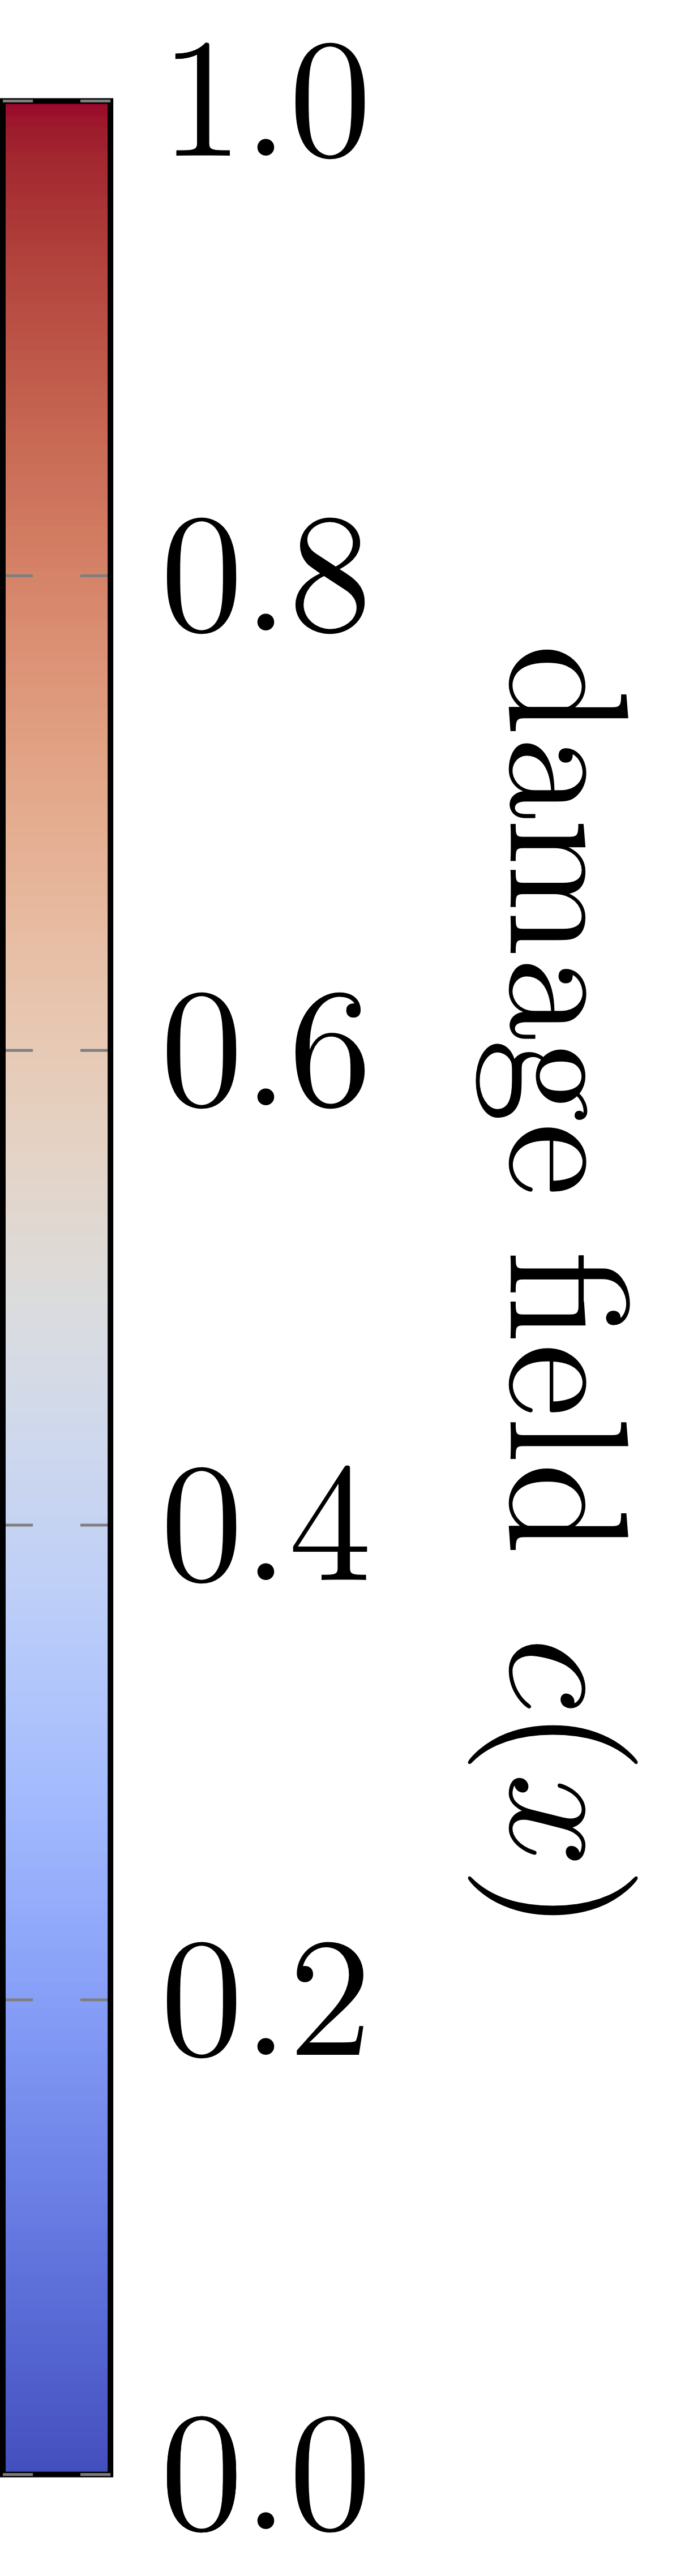
\includegraphics[width=\linewidth]{figures/fracture-damage-colorbar-label.png}
 \end{minipage}
%\caption{The final damage field for the fracture problem described in \Cref{sec:fracture}.}
%\label{fig:fracture}
% \vspace*{-1em}
\end{figure}
\end{minipage}
\end{frame}



\begin{frame}\frametitle{Finite Element Spaces I}

\begin{beamercolorbox}[rounded=true, shadow=true, wd=\textwidth]{block body}
%\begin{itemize}
%\item 
\visible<1->{$\mathcal{T}_h$ shape-regular partition of $\Omega \subset \mathbb{R}^2$.\medskip}

\visible<2->{$T \in \mathcal{T}_h$ open connected triangular mesh cells with Lipschitz boundaries $\partial T$.\medskip}

%\item
\visible<3->{$\Omega := \bigcup_{T \in \mathcal{T}_h} \overline{T}$.\medskip}

%\item 
\visible<4->{$h = \max_{T\in\mathcal{T}_h} \mathrm{diam}(T)$ is the mesh size.\medskip}

%\item 
\visible<5->{$\mathbb{P}_{p}(T)$  space of polynomials of total order up to and including $p$ on a triangle $T$.\medskip}

%%\item $\mathbb{Q}_{p}(T)$ space of tensor-product polynomials of order up to and including $p$ on a quadrilateral $T$.

%\item 
\visible<6->{$\mathbb{X}(T)$ space of polynomials over an element $T \in \mathcal{T}_h$.}
%\item We define ``broken'' polynomials 
\visible<6->{
\[
\mathbb{X}(\mathcal{T}_h) = \{\varphi \in L^\infty(\Omega) \mid \varphi_{|T} \in \mathbb{X}(T) \text{~for every~} T \in \mathcal{T}_h\}.
\]
%\item  
There is an analogous construction for quadrilaterals in the paper.}
%\end{itemize}
\end{beamercolorbox}

\end{frame}

\begin{frame}\frametitle{Finite Element Spaces II}
\begin{beamercolorbox}[rounded=true, shadow=true, wd=\textwidth]{block body}
%\begin{itemize}
%\item 
\visible<1->{We require spaces of degree-$q$ polynomials whose traces on the cell boundary $\partial T$ have lower polynomial degree $p < q$.\medskip}

%\item 
\visible<2->{Define the sets of bubble functions in $\mathbb{P}_{q}(T)$
 %and $\mathbb{Q}_{q}(T)$ 
 to be 
\[
\aligned
\mathring{\mathbb{P}}^{q}(T) &= \{ \varphi \in \mathbb{P}_{q}(T) \mid \varphi_{|\partial T} =  0\}%\\
%\mathring{\mathbb{Q}}^{q}(T) &= \{ \varphi \in \mathbb{Q}_{q}(T) \mid \varphi_{|\partial T} =  0\}
\endaligned
\]}\visible<3->{
%\item 
Then define 
\[
\aligned
\hat{\mathbb{P}}_{p}(T) &= \mathbb{P}_{p}(T) \setminus \mathring{\mathbb{P}}^{p}(T)%\\
%\hat{\mathbb{Q}}_{p}(T) &= \mathbb{Q}_{p}(T) \setminus \mathring{\mathbb{Q}}^{p}(T)
\endaligned
\]}\visible<4->{
%\item 
Finally
let
\begin{equation}
	\mathbb{P}_p^q(T) = \hat{\mathbb{P}}_{p}(T) \oplus \mathring{\mathbb{P}}^{q}(T).
%	\quad
%	\text{and}
%	\quad
%	\mathbb{Q}_p^q(T) = \hat{\mathbb{Q}}_{p}(T) \oplus \mathring{\mathbb{Q}}^{q}(T)
%	\,.
\end{equation}}\vspace{-2ex}
%\end{itemize}
\end{beamercolorbox}
\end{frame}

\begin{frame}\frametitle{Finite Element Spaces III}
\begin{minipage}{0.55\textwidth}
\begin{beamercolorbox}[rounded=true, shadow=true, wd=\textwidth]{block body}
For any integer $p \geq 1$, we define the following pairs of spaces:
%\begin{subequations}
\label{eq:SubspacePairs}
\smallskip
%\noindent\textsl{Triangular elements.} 
We refer to the following as the $(\mathbb{P}_p\text{-bubble},\mathbb{P}_{p-1}\text{-broken})$ pairing:
\begin{equation*}
\label{eq:SubspacePair1}
	V_h = \mathbb{P}_{p}^{p+2}(\mathcal{T}_h)\cap H^1_0(\Omega)
	\,,\qquad
	% \quad
	% \text{and}
	% \quad
	W_h = \mathbb{P}_{p-1}(\mathcal{T}_h)
	\,.
\end{equation*}
% \medskip
%
%\noindent\textsl{Quadrilateral elements.} We refer to the following as the $(\mathbb{Q}_p\text{-bubble},\mathbb{Q}_{p-1}\text{-broken})$ pairing:
%\begin{equation}
%\label{eq:SubspacePair2}
%	V_h = \mathbb{Q}_{p}^{p+1}(\mathcal{T}_h)\cap H^1_0(\Omega)
%	\,,\qquad
%	% \quad
%	% % V_h = \mathbb{Q}_{p+2}(\mathcal{T}_h)\cap H^1_0(\Omega)
%	% \quad
%	% \text{and}
%	% \quad
%	W_h = \mathbb{Q}_{p-1}(\mathcal{T}_h)
%	\,.
%\end{equation}
%\end{subequations}
\end{beamercolorbox}
\end{minipage}\hfill\visible<2->{
\begin{minipage}{0.4\textwidth}
\begin{example}[$p = 1$]
$V_h : $  direct sum of piecewise linear fcns.\ and  3$^{rd}$ order bubble fcns.\\ 
$W_h : $ piecewise constants. 
\end{example}

\begin{figure}
\centering
	\subcaptionbox*{$\mathbb{P}_1\text{-bubble}$}{
		\includegraphics[width=0.35\linewidth]{./figures/Elements/P1B.pdf}
	}
	\subcaptionbox*{$\mathbb{P}_0\text{-broken}$}{
		\includegraphics[width=0.35\linewidth]{./figures/Elements/P0.pdf}
	}
%	\qquad
%	\subcaptionbox*{$\mathbb{Q}_1\text{-bubble}$}{
%		\includegraphics[width=0.2\linewidth]{./figures/Elements/Q1B.pdf}
%	}
%	\subcaptionbox*{$\mathbb{Q}_0\text{-broken}$}{
%		\includegraphics[width=0.2\linewidth]{./figures/Elements/Q0.pdf}
%	}
%	\caption{
%	Conventional representation of the $(\mathbb{P}_1\text{-bubble},\mathbb{P}_0\text{-broken})$ and $(\mathbb{Q}_1\text{-bubble},\mathbb{Q}_0\text{-broken})$ finite elements in two dimensions.
%	The central degree of freedom in each element can be understood as the average over the individual mesh cell.
%	\label{fig:P1BP0}}
\end{figure}
\end{minipage}}

\visible<3->{
\begin{beamercolorbox}[rounded=true, shadow=true, wd=\textwidth]{block title}
For shape regular $\mathcal{T}_h$, these pairs of spaces are \textbf{stable} for the linearized, singularly perturbed saddle point problems.
\end{beamercolorbox}}

%\begin{itemize}
%\item
%For shape regular $\mathcal{T}_h$, these pairs of spaces are \textbf{stable} for the linearized, singularly perturbed saddle point problems.
%\item 
%The paper contains similar spaces for quadrilateral mesh cells and alternative pairs without bubble functions that are also stable.
%\end{itemize}

\end{frame}


\begin{frame}\frametitle{Lagrange Multipliers}
\begin{beamercolorbox}[rounded=true, shadow=true, wd=\textwidth]{block title}\centering
 \visible<1->{What does this have to do with what I learned in nonlinear optimization class!?}
 \end{beamercolorbox}

\begin{beamercolorbox}[rounded=true, shadow=true, wd=\textwidth]{block body}
 \visible<2->{If everything were in $\mathbb R^n$, we would have 
 \begin{enumerate}
 \item \visible<3->{$u_i \ge \varphi_i$ for a $i = 1,\dots,n$.}
 \item \visible<4->{For each $i = 1,\dots, n$, there would exist a \alert{Lagrange multiplier} $\lambda_i \ge 0$.}
 \item \visible<5->{For each $i = 1,\dots, n$, we would have a \alert{complementarity condition}:
$
 \lambda_i (u_i - \varphi_i) = 0.
$}
 \item \visible<6->{1. and 2. correspond to $u \in K$ and $\lambda \ge 0$ in the sense of $V^*$.}
 \item \visible<7->{The support condition means: Letting $\mathcal{I} := \left\{x \in \Omega : u(x) > \varphi(x)\right\}$ (\alert{inactive set})
 \[
 \int_{\mathcal{I}} \dd \lambda =  \lambda(\mathcal{I}) = \lambda(\left\{x \in \Omega : u(x) > \varphi(x)\right\}) = 0, 
 \]}\visible<8->{which is exactly what we get from the complementarity condition for $i$: $u_i > \varphi_i$.}
 \end{enumerate}}
  \hypertarget{target_lagrange}{}
\hyperlink{lagrange_mult}{\beamerbutton{go back}}
 \end{beamercolorbox}
\end{frame}


  \begin{frame}\frametitle{A Workflow for Penalty Methods}
     \visible<1->{
 \begin{beamercolorbox}[rounded=true, shadow=true, wd=\textwidth]{block title}\centering
The $\gamma$-dependent subproblems are no longer constrained. This makes both the analysis and the numerical solution more familiar to techniques for PDEs.
 \end{beamercolorbox}}\hfill
 
 \visible<2->{
 \begin{beamercolorbox}[rounded=true, shadow=true, wd=\textwidth]{block body}
\visible<3->{Theory: 
\begin{itemize}
\item \visible<4->{Prove existence and uniqueness of $u_{\gamma}$ using the Direct Method.}
\item \visible<5->{Prove that $J_{\gamma} \to J + i_{K}$ in the sense of \alert{Mosco convergence} $\Rightarrow$ $u_{\gamma} \rightharpoonup u$.}
\item \visible<6->{Prove that $J_{\gamma}$ is G\^{a}teaux differentiable and derive optimality conditions:
\[
dJ_{\gamma}(u_{\gamma}) = 0 \Leftrightarrow -\Delta u - \underbrace{\gamma \max\{0,\varphi-u\}}_{=:\lambda_{\gamma}} = f.
\]}
\end{itemize}
}\vspace{-3ex}

%\visible<7->{Algorithms:
%\begin{itemize}
%\item A standard way to compute $u_{\gamma}$ is the \alert{Semismooth Newton Method}.
%\item In a nutshell: Given $u^k \in H^1_0(\Omega)$, compute $\delta^k \in H^1_0(\Omega)$ such that
%\[
%-\Delta \delta
%\]
%\end{itemize}
%}
 \end{beamercolorbox}}
 \hypertarget{target_workflow}{}
\hyperlink{penalty}{\beamerbutton{go back to penalty}}
  \end{frame}
  
    \begin{frame}\frametitle{A Workflow for Penalty Methods}
      \visible<1->{
 \begin{beamercolorbox}[rounded=true, shadow=true, wd=\textwidth]{block title}\centering
Both theory and experience has shown that developing algorithms in infinite dimensions (usually) leads to mesh independent numerical methods after discretization.
 \end{beamercolorbox}}\hfill   
    
 \begin{beamercolorbox}[rounded=true, shadow=true, wd=\textwidth]{block body}
\visible<2->{Algorithms:
\begin{itemize}
\item \visible<2->{A standard way to compute $u_{\gamma}$ is the \alert{Semismooth Newton Method}.}
\item \visible<3->{In a nutshell: Given $u^k \in H^1_0(\Omega)$, compute $\delta^k \in H^1_0(\Omega)$ such that
\[
-\Delta \delta^k + \gamma \chi_{\{\varphi - u^k > 0\}}\delta^k = \underbrace{\Delta u^k + \gamma \max\{0, \varphi - u^k\} + f}_{=:\tt{res_k}} 
\]\vspace{-2ex}}

\visible<4->{Set $u^{k+1} := u^k + \delta^k.$ Stop when $\|{\tt res_{k+1}}\|_{H^{-1}(\Omega)} \le {\tt tol_{rel}}\|{\tt res_{0}}\|_{H^{-1}(\Omega)} + {\tt tol_{abs}}$  }
\end{itemize}
}
 \end{beamercolorbox}
  \end{frame}

\begin{frame}\frametitle{Comments I}
 \begin{beamercolorbox}[rounded=true, shadow=true, wd=\textwidth]{block body}
\visible<1->{For each fixed $\gamma > 0$, this method provably converges \alert{very fast} (locally superlinearly).\medskip}
 
 \visible<2->{Analytical path-following methods for adaptive, automatic updates of $\gamma$ are available.\medskip} 
 
 \visible<3->{But $u_{\gamma}$ is \alert{never} feasible for \alert{finite} $\gamma$. This may cause \alert{conditioning issues} as $\gamma \uparrow +\infty$.}
  \end{beamercolorbox}
  
 \visible<4->{
  \begin{beamercolorbox}[rounded=true, shadow=true, wd=\textwidth]{block body}
  There are two challenges for discretization: 
  \[\aligned
  ( \chi_{\{\varphi - u^k > 0\}}\delta^k, w) &= \int_{\{\varphi - u^k > 0\}} \delta^k w \dd x\\
  ( \max\{0, \varphi - u^k\} ,w) &= \int_{\{\varphi - u^k > 0\}}(\varphi - u^k) w \dd x
  \endaligned
  \]
 \end{beamercolorbox}
 }
\end{frame}

\begin{frame}\frametitle{Comments II}
\begin{minipage}{0.3\textwidth}\centering
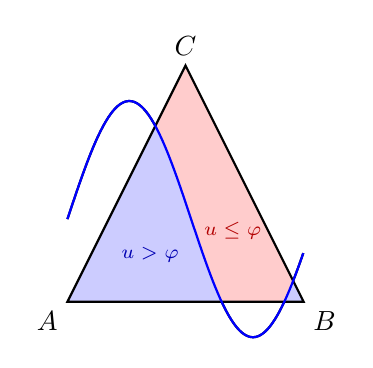
\begin{tikzpicture}[scale=3]
  % Define triangle vertices
  \coordinate (A) at (0,0);
%  \coordinate (B) at (1,0);
%  \coordinate (C) at (0.5,1);

  \coordinate (B) at (1,0);
  \coordinate (C) at (0.5,1);

  % Define curve
  \draw[name path=curve, thick, domain=0:1, samples=100, variable=\x] 
    plot ({\x}, {0.5*sin(6*\x r) + 0.35});

  % Triangle path
  \path[name path=AB] (A) -- (B);
  \path[name path=BC] (B) -- (C);
  \path[name path=CA] (C) -- (A);

  % Clip and fill region below curve inside triangle
  \begin{scope}
    \clip (A) -- (B) -- (C) -- cycle;
    \fill[blue!20] plot[domain=0:1, samples=100] 
      ({\x}, {0.5*sin(6*\x r) + 0.35}) -- (1,0) -- (0,0) -- cycle;
  \end{scope}

  % Clip and fill region above curve inside triangle
  \begin{scope}
    \clip (A) -- (B) -- (C) -- cycle;
    \fill[red!20] (0,0) -- (0.5,1) -- (1,0) -- 
      plot[domain=1:0, samples=100] 
      ({\x}, {0.5*sin(6*\x r) + 0.35}) -- cycle;
  \end{scope}

  % Draw triangle edges
  \draw[thick] (A) -- (B) -- (C) -- cycle;

  % Draw curve on top
  \draw[thick, blue] plot[domain=0:1, samples=100] 
    ({\x}, {0.5*sin(6*\x r) + 0.35});

  % Optional: label triangle vertices
  \node[below left] at (A) {$A$};
  \node[below right] at (B) {$B$};
  \node[above] at (C) {$C$};
  
 
   % Label in blue region (below the curve)
  \node[blue!70!black] at (0.35,0.2) {\scriptsize $u > \varphi$};

  % Label in red region (above the curve)
  \node[red!70!black] at (0.7,0.3) {\scriptsize $u \le \varphi$};
\end{tikzpicture}
\end{minipage}\hfill
\begin{minipage}{0.68\textwidth}
  \begin{beamercolorbox}[rounded=true, shadow=true, wd=\textwidth]{block body}
  To be computationally efficient, we need to make a choice:\medskip
  
For a cell $T$, we are given
\begin{enumerate}
\item Quadrature points $x_1,\dots,x_p$
\item Weights $w_1,\dots,w_p$
\item $N_{T} = \{1,\dots,p\}$ 
\end{enumerate}\visible<2->{
\alert{If $\varphi(x_i) - u^k(x_i) \le 0$, then $N_{T} := N_{T} \setminus \{i\}$}.}\visible<3->{
Then we use
  \[\aligned
  ( \chi_{\{\varphi - u^k > 0\}}\delta^k, v) &\approx \sum_{i \in N_{T}}w_i \delta^k(x_i) v(x_i)\\
  ( \max\{0, \varphi - u^k\} ,v) &\approx \sum_{i \in N_{T}}w_i(\varphi(x_i) - u^k(x_i)) v(x_i).
  \endaligned
  \]\vspace{-1ex}}
 \end{beamercolorbox}
\end{minipage}
\end{frame}

  \begin{frame}\frametitle{AL Workflow}
  \visible<1->{
   \begin{beamercolorbox}[rounded=true, shadow=true, wd=\textwidth]{block body}
\visible<1->{The theory for the subproblems  mirrors that of penalty methods (if $\lambda$ is regular).\medskip

\visible<2->{The optimality conditions for minimizing $L(u,\lambda,\gamma)$ are
\[
-\Delta u - \max\{0,\lambda + \gamma(\varphi - u)\} = f
\]
We can therefore compute $u_{\gamma}$ using a \alert{Semismooth Newton Method}.\medskip}

\visible<3->{We take $\gamma := \tau\gamma$ ($\tau > 1$) and \alert{update} the \alert{multipliers} $\lambda_{\gamma}$ using the formula 
\[
\lambda_{\gamma} := \lambda + \max\{0,\lambda + \gamma(\varphi - u_{\gamma})\}.
\]
}\vspace{-3ex}
}
\end{beamercolorbox}}   
  
        \visible<4->{
 \begin{beamercolorbox}[rounded=true, shadow=true, wd=\textwidth]{block title}
Ito \& Kunisch (1990) provides convergence theory for an AL method in Hilbert space that applies to the obstacle problem and a problem with gradient constraints.  \visible<3->{The theory requires more regularity of the obstacle, $\lambda \in L^2(\Omega)$, and $\gamma \to +\infty$.} \end{beamercolorbox}}\hfill   
  \end{frame}
  
  \begin{frame}\frametitle{IP Workflow}
  \visible<1->{
   \begin{beamercolorbox}[rounded=true, shadow=true, wd=\textwidth]{block body}
\visible<1->{The theory for the subproblems is more complicated than for penalty and AL.\medskip

}
\visible<2->{Logarithmic penalties are \alert{not differentiable} in the usual functions spaces.\medskip

}
\visible<3->{If there are reals $\epsilon(\mu) > 0$ and $M(\mu) > 0$ such that solution $u_{\mu} \in [\varphi + \epsilon(\mu), M(\mu)]$, then 
\begin{multline*}
\int_{\Omega} \ln(u + \eta \delta - \varphi) - \ln(u-\varphi) - \eta\frac{\delta}{u - \varphi} \dd x =
-\eta^2 \underbrace{\left(\int_{\Omega}\frac{\delta}{u - \varphi}\int_{0}^{1} \frac{1}{u - \varphi +  \tau \eta \delta} \dd \tau\dd x.\right)}_{=: A(u,\delta,\eta)}
\end{multline*}\vspace{-2ex}

is valid provided $\eta > 0$ is sufficiently small and \alert{$\delta \in H^1(\Omega) \cap L^{\infty}(\Omega)$}.\medskip

}
\visible<4->{Once we show $A(u,\delta,\eta)$ is bounded as $\eta \downarrow 0$, we can derive the \alert{optimality condition}:
\[
J_{\mu}(u_{\mu}) = 0 \Longleftrightarrow -\Delta u_{\mu} - \frac{\mu}{u_{\mu} - \varphi} = f
\]
}\vspace{-3ex}
\end{beamercolorbox}}   
  
%        \visible<4->{
% \begin{beamercolorbox}[rounded=true, shadow=true, wd=\textwidth]{block title}
%Ito \& Kunisch (1990) provides convergence theory for an AL method in Hilbert space that applies to the obstacle problem and a problem with gradient constraints.  \visible<3->{The theory requires more regularity of the obstacle, $\lambda \in L^2(\Omega)$, and $\gamma \to +\infty$.} \end{beamercolorbox}}\hfill   

\end{frame}

\begin{frame}\frametitle{Comments I}
  \visible<1->{
   \begin{beamercolorbox}[rounded=true, shadow=true, wd=\textwidth]{block body}
\visible<1->{The optimality conditions yields a \alert{singular semilinear elliptic PDE}:
\[
-\Delta u_{\mu} - \frac{\mu}{u_{\mu} - \varphi} = f
\]
This is unfortunate, especially if the Lebesgue measure of $\mathcal{A} := \left\{u = \varphi \right\}$ is positive.\medskip 
}

\visible<2->{
Introducing a slack $\lambda_{\mu} := \frac{\mu}{u_{\mu} - \varphi}$ we can write down a \alert{primal dual} formulation:
\[\aligned
-\Delta u_{\mu} - \lambda_{\mu} &= f\\
(u_{\mu}-\varphi) \lambda_{\mu} &= \mu
\endaligned
\]
This system can be solved with \alert{Newton's method} for each $\mu$.}
\end{beamercolorbox}}   
  
%        \visible<4->{
% \begin{beamercolorbox}[rounded=true, shadow=true, wd=\textwidth]{block title}
%Ito \& Kunisch (1990) provides convergence theory for an AL method in Hilbert space that applies to the obstacle problem and a problem with gradient constraints.  \visible<3->{The theory requires more regularity of the obstacle, $\lambda \in L^2(\Omega)$, and $\gamma \to +\infty$.} \end{beamercolorbox}}\hfill   

\end{frame}

\begin{frame}\frametitle{Comments II}
  \visible<1->{
   \begin{beamercolorbox}[rounded=true, shadow=true, wd=\textwidth]{block body}
\visible<1->{Find strictly feasible $(u_{\mu},\lambda_{\mu})$ satisfying
\[\aligned
-\Delta u_{\mu} - \lambda_{\mu} &= f\\
(u_{\mu}-\varphi) \lambda_{\mu} &= \mu
\endaligned
\]}\visible<2->{We need to ensure $u_{\mu} > \varphi$ and $\lambda_{\mu} > 0$ to be faithful to interior point.\medskip

This does not guarantee feasibility and will require an intelligent strategy for updating $\mu$ and a special line search at each step to guarantee primal and dual feasibility.
}
\end{beamercolorbox}}   
  
        \visible<3->{
 \begin{beamercolorbox}[rounded=true, shadow=true, wd=\textwidth]{block title}\centering
Despite its theoretical promises, IP falls short of our ideal solver. \textbf{Is there a better idea?}
\end{beamercolorbox}}\hfill   

\end{frame}

 \begin{frame}\frametitle{Experiments: Results}
 \hypertarget{target_alpha}{}  % Target anchor
\begin{minipage}{0.4\linewidth}
\begin{figure}
	\centering
	\begin{tikzpicture}
%		\node at (-3.35,0.5) {
\includegraphics[height=1.5in]{Figures/ObstacleExperiment1.png}};
		\node at (-1,0.4) {
			   \includegraphics[clip=true, trim= 0 0 0.35cm 0, height=4cm]{figures/example0_ConvergenceRate.pdf}
		};
%	    \node at (-3.5,0.4) {\includegraphics[height=2cm]{figures/colorbar0.pdf}};
%	    \node at (-2.2,-1.35) {\scriptsize $
%	    	u(x,y)
%	    	=
%	    	\begin{cases}
%	    		0 & \text{if~} x < 0\\
%	    		x^4 & \text{otherwise}\\
%	    	\end{cases}
%	    $};
    \end{tikzpicture}
%	\caption{
%	\label{fig:BiactiveIterationComplexity}
%	Biactivity.
%	Verifying the convergence orders predicted by \Cref{cor:ConvergenceRates} with the $(\mathbb{P}_1\text{-bubble},\mathbb{P}_{0}\text{-broken})$ discretization (FEniCSx).
%	Left: The exact solution.
%	Right: Plots of the optimization error $\|u_h - u_h^k\|_{H^1(\Omega_\infty)}$ and corresponding step size $\alpha_k$ when $h = h_\infty / 16$.
%	The blue curve tracks the \emph{sublinear} convergence induced by the fixed step size rule $\alpha_k = 1$.
%	Meanwhile, the step size rules \cref{eq:ObstacleStepSizes_geometric} and \cref{eq:ObstacleStepSizes_superexponential} induce \emph{linear} (red) and \emph{superlinear} (green) convergence, respectively.
%	The results are similar on finer meshes due to mesh-independence; cf.~\Cref{tab:BiactivityMeshIndependence}.
%	}
\end{figure}
\end{minipage}\qquad
\begin{minipage}{0.45\linewidth}
{\footnotesize
Proximal point is a (slow) fixed point method if $\alpha$ is left fixed. We choose:  $\alpha_1 = 1$,
\begin{equation*}
\label{eq:ObstacleStepSizes_superexponential}
	\alpha_k
	=
	\min\bigl\{ \max\bigl\{\alpha_1,r^{q^{k-1}} - \alpha_{k-1}\bigr\} , 10^{10} \bigr\}
	%\,,
	%\quad
	%k = 2,3,\ldots,
\end{equation*}
where $r = q = 1.5$.\smallskip  

Once $\alpha_k = 10^{10}$, we can check successive iterates as a stopping criterion.
}
\end{minipage}

    \hyperlink{example_1_alpha}{\beamerbutton{Back to Example 1}}
\end{frame}
  
\end{document}